%%%%%%%%%%%%%%%%%%%%%%%%%%%%%%%%%%%%%%%%%
% Classicthesis Typographic Thesis
% LaTeX Template
% Version 1.1 (4/8/12)
%
% This template has been downloaded from:
% http://www.LaTeXTemplates.com
%
% Original author:
% André Miede (http://www.miede.de)
%
% License:
% CC BY-NC-SA 3.0 (http://creativecommons.org/licenses/by-nc-sa/3.0/)
%
% General Tips:
% 1) Make sure to edit the classicthesis-config.file
% 2) New enumeration (A., B., C., etc in small caps): \begin{aenumerate} \end{aenumerate}
% 3) For margin notes: \marginpar or \graffito{}
% 4) Do not use bold fonts in this style, it is designed around them
% 5) Use tables as in the examples
% 6) See classicthesis-preamble.sty for useful commands
%
%%%%%%%%%%%%%%%%%%%%%%%%%%%%%%%%%%%%%%%%%

%----------------------------------------------------------------------------------------
%	PACKAGES AND OTHER DOCUMENT CONFIGURATIONS
%----------------------------------------------------------------------------------------

\documentclass[
		twoside,openright,titlepage,numbers=noenddot,headinclude,%1headlines,
                footinclude=true,cleardoublepage=empty,
                BCOR=5mm,paper=a4,fontsize=11pt, % Binding correction, paper type and font size
                ngerman,american, % Languages
                ]{scrreprt} 
                
% Includes the file which contains all the document configurations and packages - make sure to edit this file
%%%%%%%%%%%%%%%%%%%%%%%%%%%%%%%%%%%%%%%%%
% Thesis Configuration File
%
% The main lines to change in this file are in the DOCUMENT VARIABLES
% section, the rest of the file is for advanced configuration.
%
%%%%%%%%%%%%%%%%%%%%%%%%%%%%%%%%%%%%%%%%%

%----------------------------------------------------------------------------------------
%	DOCUMENT VARIABLES
%	Fill in the lines below to enter your information into the thesis template
%	Each of the commands can be cited anywhere in the thesis
%----------------------------------------------------------------------------------------

% Remove drafting to get rid of the '[ Date - classicthesis version 4.0 ]' text at the bottom of every page
\PassOptionsToPackage{eulerchapternumbers,
                      listings,
                      drafting,
                      pdfspacing,
                      subfig,
                      beramono,
                      eulermath,
                      parts}{classicthesis}
% Available options: drafting parts nochapters linedheaders eulerchapternumbers beramono eulermath pdfspacing minionprospacing tocaligned dottedtoc manychapters listings floatperchapter subfig
% Adding 'dottedtoc' will make page numbers in the table of contents flushed right with dots leading to them

\newcommand{\myTitle}{My Title\xspace}
%\newcommand{\mySubtitle}{My Subtitle\xspace}
\newcommand{\myDegree}{Doktor-Ingenieur (Dr.-Ing.)\xspace}
\newcommand{\myName}{Michel Steuwer\xspace}
\newcommand{\myDekan}{Prof. Dr. Martin Stein\xspace}
\newcommand{\myProf}{Prof. Dr. habil. Sergei Gorlatch\xspace}
\newcommand{\myOtherProf}{Put name here\xspace}
\newcommand{\myFaculty}{Institut for Computer Science\xspace}
\newcommand{\myDepartment}{Department for Mathematics and Computer Science\xspace}
\newcommand{\myUni}{University of M\"unster\xspace}
\newcommand{\myLocation}{M\"unster\xspace}
\newcommand{\myTime}{2014\xspace}
\newcommand{\myVersion}{Version 0.1\xspace}

\usepackage[dvipsnames]{xcolor}
\definecolor{PantoneBlack7}{cmyk}{0, 0, 0.1, 0.9}
\definecolor{Pantone877}{cmyk}{0.38, 0.27, 0.26, 0.09}
\newcommand{\mainColor}{PantoneBlack7}

%----------------------------------------------------------------------------------------
%	USEFUL COMMANDS
%----------------------------------------------------------------------------------------

\newcommand{\ie}{i.\,e.}
\newcommand{\Ie}{I.\,e.}
\newcommand{\eg}{e.\,g.}
\newcommand{\Eg}{E.\,g.} 

\newcounter{dummy} % Necessary for correct hyperlinks (to index, bib, etc.)
\providecommand{\mLyX}{L\kern-.1667em\lower.25em\hbox{Y}\kern-.125emX\@}

%----------------------------------------------------------------------------------------
%	PACKAGES
%----------------------------------------------------------------------------------------

\usepackage{lipsum} % Used for inserting dummy 'Lorem ipsum' text into the template

%------------------------------------------------
 
\PassOptionsToPackage{latin9}{inputenc} % latin9 (ISO-8859-9) = latin1+"Euro sign"
\usepackage{inputenc}
 
 %------------------------------------------------

%\PassOptionsToPackage{ngerman,american}{babel}  % Change this to your language(s)
% Spanish languages need extra options in order to work with this template
%\PassOptionsToPackage{spanish,es-lcroman}{babel}
\usepackage{babel}

%------------------------------------------------			

\PassOptionsToPackage{square,numbers}{natbib}
 \usepackage{natbib}
 
 %------------------------------------------------

\PassOptionsToPackage{fleqn}{amsmath} % Math environments and more by the AMS 
 \usepackage{amsmath}
 
 %------------------------------------------------

\PassOptionsToPackage{T1}{fontenc} % T2A for cyrillics
\usepackage{fontenc}

%------------------------------------------------

\usepackage{xspace} % To get the spacing after macros right

%------------------------------------------------

\usepackage{mparhack} % To get marginpar right

%------------------------------------------------

\usepackage{fixltx2e} % Fixes some LaTeX stuff 

%------------------------------------------------

\PassOptionsToPackage{smaller}{acronym} % Include printonlyused in the first bracket to only show acronyms used in the text
\usepackage{acronym} % nice macros for handling all acronyms in the thesis

%------------------------------------------------

%\renewcommand*{\acsfont}[1]{\textssc{#1}} % For MinionPro
\renewcommand{\bflabel}[1]{{#1}\hfill} % Fix the list of acronyms

%------------------------------------------------

\PassOptionsToPackage{pdftex}{graphicx}
\usepackage{graphicx} 

%----------------------------------------------------------------------------------------
%	FLOATS: TABLES, FIGURES AND CAPTIONS SETUP
%----------------------------------------------------------------------------------------

\usepackage{tabularx} % Better tables
\setlength{\extrarowheight}{3pt} % Increase table row height
\newcommand{\tableheadline}[1]{\multicolumn{1}{c}{\spacedlowsmallcaps{#1}}}
\newcommand{\myfloatalign}{\centering} % To be used with each float for alignment
\usepackage{caption}
\captionsetup{format=hang,font=small}
\usepackage{subfig}  

%----------------------------------------------------------------------------------------
%	CODE LISTINGS SETUP
%----------------------------------------------------------------------------------------

\usepackage{listings} 
%\lstset{emph={trueIndex,root},emphstyle=\color{BlueViolet}}%\underbar} % for special keywords
\lstset{language=[LaTeX]Tex, % Specify the language for listings here
keywordstyle=\color{RoyalBlue}, % Add \bfseries for bold
basicstyle=\small\ttfamily, % Makes listings a smaller font size and a different font
%identifierstyle=\color{NavyBlue}, % Color of text inside brackets
commentstyle=\color{Green}\ttfamily, % Color of comments
stringstyle=\rmfamily, % Font type to use for strings
numbers=left, % Change left to none to remove line numbers
numberstyle=\scriptsize, % Font size of the line numbers
stepnumber=5, % Increment of line numbers
numbersep=8pt, % Distance of line numbers from code listing
showstringspaces=false, % Sets whether spaces in strings should appear underlined
breaklines=true, % Force the code to stay in the confines of the listing box
%frameround=ftff, % Uncomment for rounded frame
frame=single, % Frame border - none/leftline/topline/bottomline/lines/single/shadowbox/L
belowcaptionskip=.75\baselineskip % Space after the "Listing #: Desciption" text and the listing box
}

%----------------------------------------------------------------------------------------
%	HYPERREFERENCES
%----------------------------------------------------------------------------------------

\PassOptionsToPackage{pdftex,hyperfootnotes=false,pdfpagelabels}{hyperref}
\usepackage{hyperref}  % backref linktocpage pagebackref
\pdfcompresslevel=9
\pdfadjustspacing=1

\hypersetup{
% Uncomment the line below to remove all links (to references, figures, tables, etc)
%draft, 
colorlinks=true, linktocpage=true, pdfstartpage=3, pdfstartview=FitV,
% Uncomment the line below if you want to have black links (e.g. for printing black and white)
%colorlinks=false, linktocpage=false, pdfborder={0 0 0}, pdfstartpage=3, pdfstartview=FitV, 
breaklinks=true, pdfpagemode=UseNone, pageanchor=true, pdfpagemode=UseOutlines,
plainpages=false, bookmarksnumbered, bookmarksopen=true, bookmarksopenlevel=1,
hypertexnames=true, pdfhighlight=/O, urlcolor=webbrown, linkcolor=RoyalBlue, citecolor=webgreen,
%------------------------------------------------
% PDF file meta-information
pdftitle={\myTitle},
pdfauthor={\textcopyright\ \myName, \myUni, \myFaculty},
pdfsubject={},
pdfkeywords={},
pdfcreator={pdfLaTeX},
pdfproducer={LaTeX with hyperref and classicthesis}
%------------------------------------------------
}   

%----------------------------------------------------------------------------------------
%	BACKREFERENCES
%----------------------------------------------------------------------------------------

\usepackage{ifthen} % Allows the user of the \ifthenelse command
\newboolean{enable-backrefs} % Variable to enable backrefs in the bibliography
\setboolean{enable-backrefs}{false} % Variable value: true or false

\newcommand{\backrefnotcitedstring}{\relax} % (Not cited.)
\newcommand{\backrefcitedsinglestring}[1]{(Cited on page~#1.)}
\newcommand{\backrefcitedmultistring}[1]{(Cited on pages~#1.)}
\ifthenelse{\boolean{enable-backrefs}} % If backrefs were enabled
{
\PassOptionsToPackage{hyperpageref}{backref}
\usepackage{backref} % to be loaded after hyperref package 
\renewcommand{\backreftwosep}{ and~} % separate 2 pages
\renewcommand{\backreflastsep}{, and~} % separate last of longer list
\renewcommand*{\backref}[1]{}  % disable standard
\renewcommand*{\backrefalt}[4]{% detailed backref
\ifcase #1 
\backrefnotcitedstring
\or
\backrefcitedsinglestring{#2}
\else
\backrefcitedmultistring{#2}
\fi}
}{\relax} 

%----------------------------------------------------------------------------------------
%	AUTOREFERENCES SETUP
%	Redefines how references in text are prefaced for different 
%	languages (e.g. "Section 1.2" or "section 1.2")
%----------------------------------------------------------------------------------------

\makeatletter
\@ifpackageloaded{babel}
{
\addto\extrasamerican{
\renewcommand*{\figureautorefname}{Figure}
\renewcommand*{\tableautorefname}{Table}
\renewcommand*{\partautorefname}{Part}
\renewcommand*{\chapterautorefname}{Chapter}
\renewcommand*{\sectionautorefname}{Section}
\renewcommand*{\subsectionautorefname}{Section}
\renewcommand*{\subsubsectionautorefname}{Section}
}
\addto\extrasngerman{
\renewcommand*{\paragraphautorefname}{Absatz}
\renewcommand*{\subparagraphautorefname}{Unterabsatz}
\renewcommand*{\footnoteautorefname}{Fu\"snote}
\renewcommand*{\FancyVerbLineautorefname}{Zeile}
\renewcommand*{\theoremautorefname}{Theorem}
\renewcommand*{\appendixautorefname}{Anhang}
\renewcommand*{\equationautorefname}{Gleichung}
\renewcommand*{\itemautorefname}{Punkt}
}
\providecommand{\subfigureautorefname}{\figureautorefname} % Fix to getting autorefs for subfigures right
}{\relax}
\makeatother

%----------------------------------------------------------------------------------------

\usepackage{classicthesis} 

%----------------------------------------------------------------------------------------
%	CHANGING TEXT AREA 
%----------------------------------------------------------------------------------------

%\linespread{1.05} % a bit more for Palatino
%\areaset[current]{312pt}{761pt} % 686 (factor 2.2) + 33 head + 42 head \the\footskip
%\setlength{\marginparwidth}{7em}%
%\setlength{\marginparsep}{2em}%

%----------------------------------------------------------------------------------------
%	USING DIFFERENT FONTS
%----------------------------------------------------------------------------------------

%\usepackage[oldstylenums]{kpfonts} % oldstyle notextcomp
%\usepackage[osf]{libertine}
%\usepackage{hfoldsty} % Computer Modern with osf
%\usepackage[light,condensed,math]{iwona}
%\renewcommand{\sfdefault}{iwona}
%\usepackage{lmodern} % <-- no osf support :-(
%\usepackage[urw-garamond]{mathdesign} %<-- no osf support :-(


\begin{document}

\frenchspacing % Reduces space after periods to make text more compact

\raggedbottom % Makes all pages the height of the text on that page

\selectlanguage{american} % Select your default language - e.g. american or ngerman

%\renewcommand*{\bibname}{new name} % Uncomment to change the name of the bibliography
%\setbibpreamble{} % Uncomment to include a preamble to the bibliography - some text before the reference list starts

\pagenumbering{roman} % Roman page numbering prior to the start of the thesis content (i, ii, iii, etc)

\pagestyle{plain} % Suppress headers for the pre-content pages

%----------------------------------------------------------------------------------------
%	PRE-CONTENT THESIS PAGES
%----------------------------------------------------------------------------------------

% Title Page

\begin{titlepage}

\begin{addmargin}[-1cm]{-3cm}
\begin{center}
\large

\hfill
\vfill

\begingroup
\color{Maroon}\spacedallcaps{\myTitle} \\ \bigskip % Thesis title
\endgroup

\spacedlowsmallcaps{\myName} % Your name

\vfill


\includegraphics[width=6cm]{gfx/TFZsuperellipse_bw} \\ \medskip % Picture

\mySubtitle \\ \medskip % Thesis subtitle
%\myDegree \\
\myDepartment \\
\myFaculty \\
\myUni \\ \bigskip

\myTime

\vfill

\end{center}
\end{addmargin}

\end{titlepage}
 % Main title page

% Back of the title page

\thispagestyle{empty}

\hfill

\vfill

\noindent\myName: \textit{\myTitle,} \mySubtitle, %\myDegree, 
\textcopyright\ \myTime

% You may wish to do something with the back of the title page, such as including your supervisors, location or time frame of the work. Below is an example of doing so although you may want to tweak it to your liking.

%\bigskip

%\noindent\spacedlowsmallcaps{Supervisors}: \\
%\myProf \\
%\myOtherProf \\ 
%\mySupervisor

%\medskip \\

%\noindent\spacedlowsmallcaps{Location}: \\
%\myLocation

%\medskip \\

%\noindent\spacedlowsmallcaps{Time Frame}: \\
%\myTime
 % Back of the title page

\cleardoublepage% Abstract

\pdfbookmark[1]{Abstract}{Abstract} % Bookmark name visible in a PDF viewer

\begingroup
\let\clearpage\relax
\let\cleardoublepage\relax
\let\cleardoublepage\relax

\chapter*{Abstract} % Abstract name

Short summary of the contents\dots

\endgroup			

\vfill % Abstract page

\cleardoublepage% Publications - a page listing research articles written using content in the thesis

\pdfbookmark[1]{Publications}{Publications} % Bookmark name visible in a PDF viewer

\chapter*{Publications} % Publications page text

This thesis is based on ideas which have been described in the following publications:

\bigskip

\nocite{SteuwerKeGo2010}
\nocite{SteuwerKeGo2011}
\nocite{KesslerGoEmDaStKe2011}
\nocite{SteuwerGoBuBr2012}
\nocite{SteuwerKeGo2012}
\nocite{SteuwerKeGo2012a}
\nocite{KegelStGo2013}
\nocite{SteuwerGo2013}
\nocite{SteuwerGo2013a}
\nocite{SteuwerFrAlGo2014}
\nocite{OlejnikStGoHe2014}
\nocite{GorlatchSt2014}
\nocite{SteuwerHaBrGo2014}
\nocite{BreuerStGo2014}
\nocite{SteuwerGo2014}

% Highlight my Name in bold
\DeclareNameFormat{author}{%
\ifthenelse{\equal{#1}{Steuwer}}%
    {{\bfseries\ifblank{#4}{}{#4\space}#1}}%
    {\ifblank{#4}{}{#4\space}#1}%
\ifthenelse{\value{listcount}<\value{liststop}}%
    {\addcomma\space}
    {}}

\defbibenvironment{nonumbers}
  {\list{}
    {\setlength{\leftmargin}{\bibhang}%
     \setlength{\itemindent}{-\leftmargin}%
     \setlength{\itemsep}{\bibitemsep}%
     \setlength{\parsep}{\bibparsep}}}
  {\endlist}
  {\item}

\printbibliography[env=nonumbers,heading=none,sorting=ynt,omitnumbers=true,keyword=based-on]

% No longer highlight my Name in bold
\DeclareNameFormat{author}{%
    \ifblank{#4}{}{#4\space}#1%
\ifthenelse{\value{listcount}<\value{liststop}}%
    {\addcomma\space}
    {}}
 % Publications from the thesis page

\cleardoublepage% Acknowledgements

\pdfbookmark[1]{Acknowledgements}{Acknowledgements} % Bookmark name visible in a PDF viewer

\begingroup

\let\clearpage\relax
\let\cleardoublepage\relax
\let\cleardoublepage\relax

\chapter*{Acknowledgements} % Acknowledgements section text

Sergei Gorlatch and Christophe Dubach\\

% Muenster
Philipp Kegel
Alexander Ploss
Frank Glinka
Dominik Meil{\"a}nder
Sebastian Albers
Tim Humernbrum
Michael Haidl
Ari Rasch

Mohammed Nsaif

Waldemar Gorus
Julia Kaiser-Mariani

Benjamin Risse
Sven Strothoff

% Edinburgh
Christophe Dubach
Thibaut Lutz
Christian Fensch
Murray Cole

HiPEAC

% Lehre
% All students participating in the 14 courses I co-supervised during my stay in Muenster.
Tobias G{\"u}nnewig
Stefan Breuer
Jan-Gerd Tenberge
Michael Olejnik
Matthias Buss
Markus Blank-Burian
Sebastian Missbach
Patrick Schiffler
Malte Friese
Kai Kientopf
Matthias Droste
Florian Quinkert
Julian Buscher
Wadim Hamm
Lars Klein

% Family
Family


\endgroup
 % Acknowledgements page

\pagestyle{scrheadings} % Show chapter titles as headings

\cleardoublepage% Table of Contents - List of Tables/Figures/Listings and Acronyms

\refstepcounter{dummy}

\pdfbookmark[1]{\contentsname}{tableofcontents} % Bookmark name visible in a PDF viewer

\setcounter{tocdepth}{2} % Depth of sections to include in the table of contents - currently up to subsections

\setcounter{secnumdepth}{3} % Depth of sections to number in the text itself - currently up to subsubsections

\manualmark
\markboth{\spacedlowsmallcaps{\contentsname}}{\spacedlowsmallcaps{\contentsname}}
\tableofcontents 
\automark[section]{chapter}
\renewcommand{\chaptermark}[1]{\markboth{\spacedlowsmallcaps{#1}}{\spacedlowsmallcaps{#1}}}
\renewcommand{\sectionmark}[1]{\markright{\thesection\enspace\spacedlowsmallcaps{#1}}}

\clearpage

\begingroup 
\let\clearpage\relax
\let\cleardoublepage\relax
\let\cleardoublepage\relax

%----------------------------------------------------------------------------------------
%	List of Figures
%----------------------------------------------------------------------------------------

\refstepcounter{dummy}
%\addcontentsline{toc}{chapter}{\listfigurename} % Uncomment if you would like the list of figures to appear in the table of contents
\pdfbookmark[1]{\listfigurename}{lof} % Bookmark name visible in a PDF viewer

\listoffigures

\vspace*{8ex}
\newpage

%----------------------------------------------------------------------------------------
%	List of Tables
%----------------------------------------------------------------------------------------

\refstepcounter{dummy}
%\addcontentsline{toc}{chapter}{\listtablename} % Uncomment if you would like the list of tables to appear in the table of contents
\pdfbookmark[1]{\listtablename}{lot} % Bookmark name visible in a PDF viewer

\listoftables
        
\vspace*{8ex}
\newpage
    
%----------------------------------------------------------------------------------------
%	List of Listings
%---------------------------------------------------------------------------------------- 

\refstepcounter{dummy}
%\addcontentsline{toc}{chapter}{\lstlistlistingname} % Uncomment if you would like the list of listings to appear in the table of contents
\pdfbookmark[1]{\lstlistlistingname}{lol} % Bookmark name visible in a PDF viewer

\renewcommand*{\lstlistlistingname}{List of Listings}
\lstlistoflistings 

\vspace*{8ex}
\newpage
       
% %----------------------------------------------------------------------------------------
% %	Acronyms
% %----------------------------------------------------------------------------------------
% 
% \refstepcounter{dummy}
% %\addcontentsline{toc}{chapter}{Acronyms} % Uncomment if you would like the acronyms to appear in the table of contents
% \pdfbookmark[1]{Acronyms}{acronyms} % Bookmark name visible in a PDF viewer
% 
% \markboth{\spacedlowsmallcaps{Acronyms}}{\spacedlowsmallcaps{Acronyms}}
% 
% \chapter*{Acronyms}
% 
% \begin{acronym}[UML]
% \acro{DRY}{Don't Repeat Yourself}
% \acro{API}{Application Programming Interface}
% \acro{UML}{Unified Modeling Language}
% \end{acronym}  

\endgroup

\cleardoublepage
 % Contents, list of figures/tables/listings and acronyms

\pagenumbering{arabic} % Arabic page numbering for thesis content (1, 2, 3, etc)

\cleardoublepage % Avoids problems with pdfbookmark

%----------------------------------------------------------------------------------------
%	THESIS CONTENT - CHAPTERS
%----------------------------------------------------------------------------------------

\part{Introduction}
% Chapter 1: Introduction

\chapter{Introduction} % Chapter title

\label{ch:introduction} % For referencing the chapter elsewhere, use \autoref{ch:name}

Computer architectures have radically changed in the last 20 years with the introduction of thread-level parallelism in the form of multi-core architectures in almost all areas of computing:
from mobile computing to data centers and high-performance computing.
Furthermore, recently novel types of specialized architectures have been developed featuring large amounts of processing units for dealing with massively data-parallel workloads.
Parallelism and specialization are seen by many computer architects as two crucial answers for overcoming the challenges of increasing performance while at the same time increasing the energy efficiency~\cite{}.

% The development of mainstream programming languages and models have not kept pace with the hardware development.
These modern parallel processors are often still programmed with programming languages developed in the 1980's, like Java or C++, or even older languages like C (from the 1970's) or Fortran (from the 1950's).
These languages have a simplified view of the underlying hardware architecture often more or less directly resembling the Von Neuman architecture.
Multiple cores are programmed with libraries providing \emph{threads} where the programmer explicitly controls the computations on each core which execute the program in parallel.
This style of programming has turned out to be extremely difficult, as threads running concurrently on distinct cores can modify shared data which can lead to serious problems like deadlocks and non-determinism.
Even if the programmer develops a correct parallel implementation, optimizing this implementation for modern parallel processors is a challenging task even for experienced programmers.
Due to the lack of better programming systems, programmers are currently forced to develop hardware-specific implementations optimized towards a particular hardware architecture to achieve high performance.

This thesis describes our work to address these issues.
In the first part of the thesis we present a high-level programming model and its implementation which is designed to simplify the programming of modern parallel processors, especially systems comprising multiple Graphics processing units (\GPUs).
In the second part we discuss a system which generates high-performance code for different modern parallel processors, particularly a multi-core \CPU and two different types of \GPUs, from a single high-level program representation.
In the final part of the thesis we will outline how these two systems can be combined in the future to obtain a programming system which simplifies programming and achieves high-performance on different hardware architectures.

\noindent
We will start our discussion with an introduction on programming of modern parallel processors.
From this we will identify the two main challenges we tackle in this thesis:
the programmability challenge and the performance portability challenge.
We will then list our contributions before presenting the outline for the rest of the thesis.

\section{Multi-Core Processors and their Programming}

% processors become parallel
Traditionally, the performance of microprocessors has been mainly increased by boosting the clock frequency, optimize the execution flow, and improve caches~\cite{Sutter2005}.
This development has drastically changed around 10 years ago, as shown in \autoref{fig:cpuTrend}.
While the number of transistors continues to grow according to Moore's Law~\cite{Moore1998} the clock frequency and power consumption have hit a plateau around 2005.
\begin{figure}
  \centering
  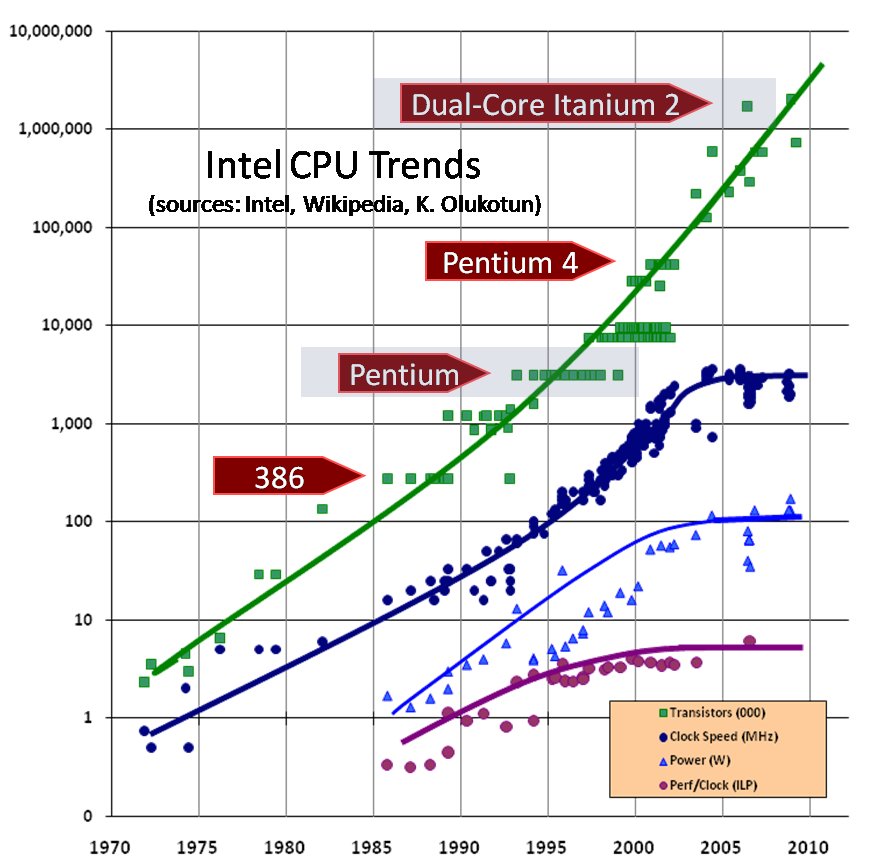
\includegraphics[width=.9\linewidth]{Figures/CPUTrend.png}
  \caption{Development of Intel CPU over time. Inspired by~\cite{Sutter2005}}
  \label{fig:cpuTrend}
\end{figure} \todo{replace figure}
The reason for this lies in multiple physical effects, especially the physical limit of signal speed and increased heat development, which is mainly due to increased power consumption, both of which limit further increases of the clock frequency.
The predominant answer to this challenge has been the introduction of multiple distinct \emph{cores} which can operate concurrently.
% parallelism is now explicit to the programmer
Parallelism has been exploited in computer architectures for a long time at the bit level and the instruction level, but different than before with the introduction of multiple cores, this new \emph{thread-level parallelism} is explicit to the programmer.
This has profound effects on the design and development of software running on modern multi-core processors.
% programming with threads is a terrible idea
Most programming languages allow programmers to exploit multiple cores by the means of \emph{threads}.
A thread is a sequence of instructions defined by the programmer which can be scheduled by the runtime to be executed on a particular core.
Multiple threads can be executed concurrently and the programmer is responsible to use synchronization primitives, like locks or semaphores, for coordinating the execution of multiple threads.
Programming with threads is widely regarded as extremely difficult~\cite{} as subtle problems can arise which are hard to detect but can have severe consequences.
Nevertheless, threads are still the de-facto standard for programming multi-core \CPUs.

\bigskip

\noindent
% still moores law, no dennards scaling
% new hardware trend driven by energy efficiency, specialization, a.k.a heterogeneity, most prominent example: GPUs
While Moore's law still holds and transistor counts increase by further shrinking the transistor size, a related observation, known as Dennard scaling~\cite{DennardRiBaLe1974}, has broken down.
Dennard scaling suggested that power consumption is proportional with the area used for transistors on the chip.
Combined with Moore's law this meant, that the energy efficiency of processors doubled roughly every 18 month.
The primary reason for the breakdown of Dennard scaling around 2005 are physical effects appearing at the small scale of modern transistors, especially current leakage and increased heat development.
This has lead to architectures particular focused on their energy efficiency, the most prominent example of such architectures are modern Graphics Processing Units (\GPUs).
Originally developed for accelerating the rendering of complex graphics and 3D scenes, \GPUs architectures have been recently generalized to support more general purpose computations.
Some people refer to this development using the term general-purpose computing on graphics processing units (\GPGPU).

Technically \GPU architectures are multi-core architectures like modern multi-core \CPUs, but each individual core on a \GPU typically has dozens or hundreds of function units which can perform computations in parallel following the single instruction, multiple data (SIMD) principle.
These type of architectures are optimized towards a high throughput of computations, therefore, they focus on performing a large amount of operations in parallel and feature no, or only small, caches to prevent or mitigate latencies of the memory:
if a thread stalls wanting for the memory, another thread takes over and keeps the core busy.
For multi-core \CPUs switching between threads is more expensive, therefore, \CPUs are instead optimized to avoid long latencies when accessing the memory with a deep cache hierarchy and advanced architectural features, like long pipelines and out-of-order execution, all of which is designed to keep each core busy.

\section{The Programmability Challenge}

% programming on the CPU is a nightmare
Developing parallel programs for modern parallel processors is a challenging task.
The dominant approach for programming multi-core \CPUs is using multi-threading, \ie, explicitly managing the individual execution paths (called \emph{threads}) in a single program.
Threads communicate via a shared memory, where all threads have the possibility to modify any data item.
This fundamental principle gives the programmer much control over the interaction of the threads but greatly complicates the reasoning about the programs behavior.
The extensive and explicit control directly implies a very low level of abstraction, where the programmer deals with many details of the execution explicitly.
This makes the development of programs using threads complex and certain types of bugs more likely like deadlocks and data-races where the computed result depends on the order the threads are executed.
This ultimately leads to extensive problem during the development cycle as well as possible non-deterministic and undesirable behavior at runtime.

% not better on the GPU
Programming of \GPUs requires a different programming approach, as it is obviously infeasible to manage thousands of threads explicitly.
\CUDA~\cite{CUDAProgrammingGuide} and \OpenCL~\cite{OpenCL} are the two most popular approaches for programming \GPUs.
Both approaches are quite similar and require the programmer to write a function, called \emph{kernel}, which will be executed in parallel on the \GPU.
The kernel usually contains source code for identifying the thread executing the kernel which is used to coordinate on which data each thread operate on.
While this Single Program, Multiple Data (SPMD) programming model makes the management of threads feasible it does not address most problems associated with the low-level programming with threads.
For example, is explicit synchronization of threads still required and problems like deadlocks and race-conditions can still easily occur.
Furthermore, \GPU programming currently involves extensive boilerplate code to manage the execution on the \GPU, including the compilation of the kernel (in \OpenCL), transferring data to and from the \GPU, and launching the kernel by explicit specifying the number of threads to be started in parallel.

% There is a challenge: Programmability
All of this leads to our first central research question:
can we design a programming approach which significantly raise the level of abstraction and, thus, greatly simplify the development process of parallel applications, without sacrificing high-performance on multi-core \CPUs and \GPUs?
We will underpin the necessity to address this challenge with an extensive study of state-of-the-art \GPU programming using a concrete application example in \autoref{chapter:skelcl}.

In \autoref{part:skelcl} of this thesis, we will introduce, discuss, and evaluate a novel high-level programming model which attempts to address this \emph{challenge of programmability}.

\section{The Performance Portability Challenge}

% extracting performance is hard and not always predictable
Developing functional correct parallel applications for multi-core \CPUs or \GPUs is very challenging as we discussed in the preceding subsection.
Unfortunately, is the development of high-performing optimized applications even more demanding -- even for experienced programmers.
Applying optimizations often requires substantial restructuring of existing code.
Optimizations are often applied ad-hoc following certain ``rules of thumb'' derived from small-scale profiling and experiments as well as previously gained experience.
There exist no widely established approach for performing optimizations more systemically.
Especially, the performance implications of an assumed optimization is currently not predictable:
sometimes supposed optimizations leads to actual slowdowns in certain circumstances.

% compilers do a good job on low-level stuff, but fail for high-level optimizations
Modern optimizing compilers perform very sophisticated low-level optimizations, including various loop optimizations and optimization on data-flow analysis.
For all these type of optimizations, the compiler first has to recover parts of the high-level program semantics using analysis before applying the optimization.
As this analysis quickly becomes very complex compilers are ultimately limited in their optimization capabilities.
High-level optimizations which might restructure the entire source code are often out of the reach of low-level compiler optimizations and requires explicit and often extensive manual refactoring.
The state-of-the-art optimizing compilers simply are lacking the semantic high-level information necessary for performing these king of optimizations.

% optimizations are hardware-specific
Many optimizations exploit hardware-specific features and are, therefore, inherently not portable across hardware architectures.
As in current low-level programing model programmers encode these optimizations directly, programmers are forced with trade offs of either fully optimize their code for performance -- at the expense of code portability -- or implement a portable version -- at the expense of missing out on the highest performance possible.
Nowadays, programmers often choose a middle ground where introduce conditionals and branches in their code to select optimizations for the given hardware, while maintaining portability.
This, obviously, complicates the development process and decreases the maintainability of the software.

% There is a challenge: Performance Protability
This leads to our second central research question:
can we design a systematic approach where highly optimized, hardware-specific code is generated from a single high-level program representation?
We will confirm the lack of portability of performance in current state-of-the-art programming approaches using a study comparing optimizations on three different hardware architectures in \autoref{chapter:codeGeneration}.

In \autoref{part:codeGeneration} of this thesis, we will introduce, discuss, and evaluate a novel systematic code generation approach which attempts to address this \emph{challenge of performance portability}.


\section{Contributions of this Thesis}

This thesis makes the following four major contributions:

\subsection*{\hspace{2em}For Addressing the programmability challenge:}

\begin{description}
  \item[A High-level programming model for mutli-\GPU systems]\hfill\\[-1em]
    We present the design and implementation of our high-level programming model \SkelCL for programming multi-\GPU systems.
    \SkelCL offers three high-level features for simplified programming: container data types, algorithmic skeletons, and data distributions.
    We discuss our \Cpp library implementation of the \SkelCL programming model which is deeply integrated with \Cpp.
    Finally, we evaluate the level of abstraction and runtime performance of \SkelCL using a set of application studies.

  \item[Two novel algorithmic skeletons]\hfill\\[.25em]
    We introduce two novel algorithmic skeletons specialized towards \emph{allpairs} and \emph{stencil} computations.
    We present their formal definitions and discuss possible use cases in real world applications.
    For the allpairs skeleton we identify and formally define an optimization rule, which enables a more efficient implementation on \GPUs.
    We discuss and evaluate efficient implementations for both skeletons on a multi-\GPU system.
\end{description}

\subsection*{\hspace{2em}For Addressing the performance portability challenge:}

\begin{description}
  \item[A formal system for rewriting pattern-based programs]\hfill\\[-1em]
    We introduce a novel system comprising of set of high-level and low-level patterns along with a set of rewrite rules.
    The rewrite rules express high-level algorithmic and low-level optimization choices which can be systematically applied to transform a program expressed with our functional patterns.
    We proof the soundness of our approach by showing, that applying the rewrite rules does not change the program semantics.

  \item[A code generator offering performance portability]\hfill\\[.25em]
    Based on our formal rewrite system we present a novel code generator which generates from a single pattern-based program highly efficient \OpenCL code for three different hardware architectures:
    one multi-core \CPU and two different \GPUs.
    We discuss the design of our code generator and evaluate the performance of the generated \OpenCL code compared against highly optimized library code.
\end{description}

\section{Outline of this Thesis}
The remainder of this thesis is structured as follows.

\subsection*{Part I -- Introduction}

\paragraph{\autoref{chapter:background}} provides an introduction into the aspects of programming modern multi-core \CPUs and \GPUs.
We will start with the hardware where we mainly focus on \GPUs, discuss their architectures in detail, the state-of-the-art programming approaches, and optimization opportunities.
We will then shift our focus and discuss the algorithmic skeleton parallel programming model including its roots in functional programming.


\subsection*{Part II -- \SkelCL}

\paragraph{\autoref{chapter:skelcl}} addresses the programmability challenge identified in this chapter by introducing our novel \SkelCL high-level programming model targeted towards multi-\GPU systems and its implementation as a \Cpp library.
We will start by further motivating the need for high-level abstractions to simplify the software development process.
Then we present \SkelCL's three high-level features:
1) parallel container data types, 2) algorithmic skeletons, and 3) data distributions.
The combination of these features greatly simplifies the programming of multi-\GPU applications.
Finally, we will discuss the \SkelCL library implementation which is nicely integrated with \Cpp.

\paragraph{\autoref{chapter:skelcl-evaluation}} evaluates the \SkelCL programming model and library using multiple application studies.
We will start with discussing typical benchmark applications like the mandelbrot set computation and benchmarks from linear algebra.
We then continue with discussing more advanced applications from different areas, including image processing, medical imaging, physics, and bioinformatics.
We evaluate the increase of programmability and the performance of \SkelCL compared with implementations written in using the state-of-the-art \OpenCL programming approach.


\subsection*{Part III -- Code Generation using Patterns}

\paragraph{\autoref{ch:fifth}} addresses the performance portability challenge identified in this chapter by introducing a novel approach for generating highly optimized device-specific code from a single high-level program representation.
We will start the chapter with a study showing that optimizations in \OpenCL are not portable across different hardware architectures.
This emphasizes the motivation for performance portability to preserve maintainability while increase performance and efficiency at the same time.
Then we discuss the design of our code generation approach consisting of a set of parallel patterns combined with a set of rewrite rules.
The rewrite rules allow to rewrite pattern-based programs without changing their semantics which we will formally show.
Finally, we discuss how the rewrite rules can be systematically applied to optimize pattern-based programs for a particular hardware architecture.

\paragraph{\autoref{ch:sixth}} evaluates our code generation approach using a set of benchmark applications.
We evaluate the performance of the code generated using our approach and compare it against highly tuned library code on three different hardware architectures.

\subsection*{Part IV -- Summary \& Conclusions}

\paragraph{\autoref{ch:seventh}} summarizes Part II and Part II and describes their relation.
We will discuss how \SkelCL, presented in Part II, could be combined in the future with the code generator, presented in Part III, to obtain a system offering both high-level abstractions to simplify programming and high-performance on different hardware architectures.

\paragraph{\autoref{ch:eighth}} concludes the thesis by comparing against related work and discussing possible future extensions of our research.


% Chapter 2: Background

\chapter{Background} % Chapter title

\label{chapter:background}
\label{chapter:state-of-the-art}

In this chapter we will introduce and discuss the technical background of this thesis.

We will start by discussing the structure and functionality of multi-core \CPUs and \GPUs.
We will focus on \GPUs as their architecture is quite different to traditional \CPUs, and because \GPUs will be the main hardware target of our \SkelCL programming model presented later.
Then we will discuss the most common programming approaches for multi-core \CPUs and \GPUs, with a particular focus on \OpenCL.

We will then introduce the idea of structured parallel programming and discuss its origin in functional programming.
In this approach, predefined parallel patterns (\aka, \emph{algorithmic skeletons}) hiding the complexities of parallelism are used for expressing parallel programs.
This thesis builds upon this idea, developing a structured parallel programming model for \GPUs and a novel compilation technique that transforms pattern-based programs to efficient hardware-specific implementations.
% We will finish this chapter by discussing several state-of-the-art implementations of structured parallel programming for cluster systems and multi-core \CPUs.

\section{Modern Parallel Processors}
% structure and functionality of:
As discussed in the introduction in \autoref{ch:introduction}, virtually all modern processors feature multiple cores to increase their performance and energy efficiency.
Here we will look at two major types of modern parallel processors: multi-core \CPUs and \GPUs.
Multi-core \CPUs are \emph{latency-oriented} architectures~\cite{GarlandK10}, \ie, they are optimized to hide memory latencies with large caches and various other advanced architectural features, like out-of-order execution and extensive branch prediction.
\GPUs are \emph{throughput-oriented} architectures~\cite{GarlandK10}, \ie, they are optimized to increase the overall computational throughput of many parallel tasks instead of optimizing single task performance.

We will discuss both architectures in the following two sections.

\subsection{Multi-Core \CPUs}
% multi-core CPUs
\autoref{fig:multicore} shows an abstract representation of a typical multi-core \CPU architecture, like Intel's latest \CPU architecture: Haswell.
\begin{figure}
  \centering
  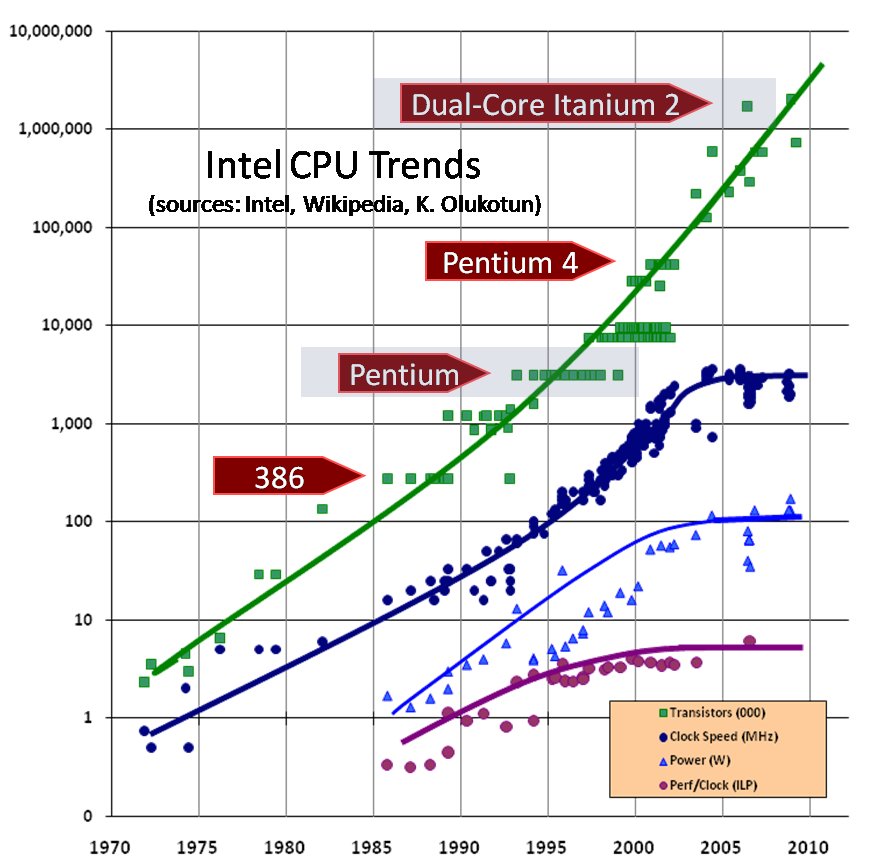
\includegraphics[width=.75\textwidth]{CPU}
  \caption{Multi-core \CPU architecture.}
  \label{fig:multicore}
\end{figure}
% describe caches
The \CPU is divided into multiple cores each of which features two levels of caches.
The smallest but fastest cache is called L1 cache and is typically divided into a distinct cache for instructions and a data cache, each of 32 kilobyte for the Haswell architecture.
Each core also features a second level cache (L2 cache) of 256 kilobyte for the Haswell architecture.
The \CPU has a large cache (L3 cache) which is shared by all cores.
This cache is often several megabytes large, for Intel's Haswell architecture the L3 cache is at least 2 and up to 45 megabytes in size.

% describe core: branch prediction, out-of-order execution, SIMD units
Each \CPU core performs computations completely independently of the other cores, and it consists itself of multiple execution units which can perform computations in parallel.
This happens transparently to the programmer even when executing a sequential program.
The \CPU core exploits \emph{instruction level parallelism} (ILP) by performing out-of-order execution which re-orders instructions prior to execution while still respecting their dependencies:
\eg, if two or more instructions have no dependencies then they can be executed in parallel.
In the Intel Haswell architecture, 4 arithmetic operations and 4 memory operations can be performed in parallel in one clock cycle on every core.
Furthermore, most modern \CPU architectures support SIMD vector extensions like the \emph{Advanced Vector Extensions} (AVX) or the older \emph{Streaming SIMD Extensions} (SSE).
These extensions add additional instructions to the instruction set architecture, allowing the compiler to generate code which explicitly groups data into vectors of a small fixed size on which operations can be executed in parallel.
The current AVX extension allows vectors of up to 256 bits, \eg, a grouping of 8 single precision floating point numbers, to be processed in parallel.
Most modern optimizing compilers perform some form of automatic vectorization, but often programmers vectorize programs manually when the compiler fails to generate sufficient by optimized code.

% make conclusions: latency oriented => caches important, good performance for single and multiple threads, comparably low core count and hyper threading -> limited thread-level parallelism
The design of multi-core \CPUs is motivated by the overall goal to provide high performance when executing multi-threaded programs and still have a high single-core performance when executing sequential programs~\cite{GarlandK10}.
This is why the individual cores have a quite sophisticated design to achieve executing a series of instructions as fast as possible, by applying out-of-order execution and exploiting architectural features like a deep pipeline for decoding and executing instructions combined with advanced branch prediction.
Unfortunately, the design of these complex cores makes switching between the threads running on the same core relatively expensive, as the execution pipeline has to be flushed and the register content for the first thread has to be saved before resuming the execution on the second thread.
To address this issue, some multi-core architectures feature \emph{Simultaneous Multi-Threading} (SMT), \aka \emph{hyper threading}:
a single \CPU core can execute multiple (usually 2 or 4) threads in parallel and switching between the threads is cheap.
Tis technique is used to mitigate the effect which memory latency can have on the execution:
if a thread is waiting for a memory request then another thread can continue executing.
The other central component used to prevent waiting times for memory requests is the cache hierarchy.
As we will see, multi-core \CPUs feature considerably larger caches than \GPUs.
The caches help to keep the threads running in parallel on the multi-core \CPU busy.

% Possible optimizations
Among the most important optimizations to achieve high performance on modern multi-core \CPUs are:
exploiting the SIMD vector extensions and optimizing the cache usage~\cite{IntelCPUOptimizingGuide}.

\subsection{Graphics Processing Units}
  % GPUs
\autoref{fig:gpu} shows an abstract representation of a typical \GPU architecture, like Nvidia's latest \GPU architecture for the high-performance computing market: Kepler.
\begin{figure}
  \centering
  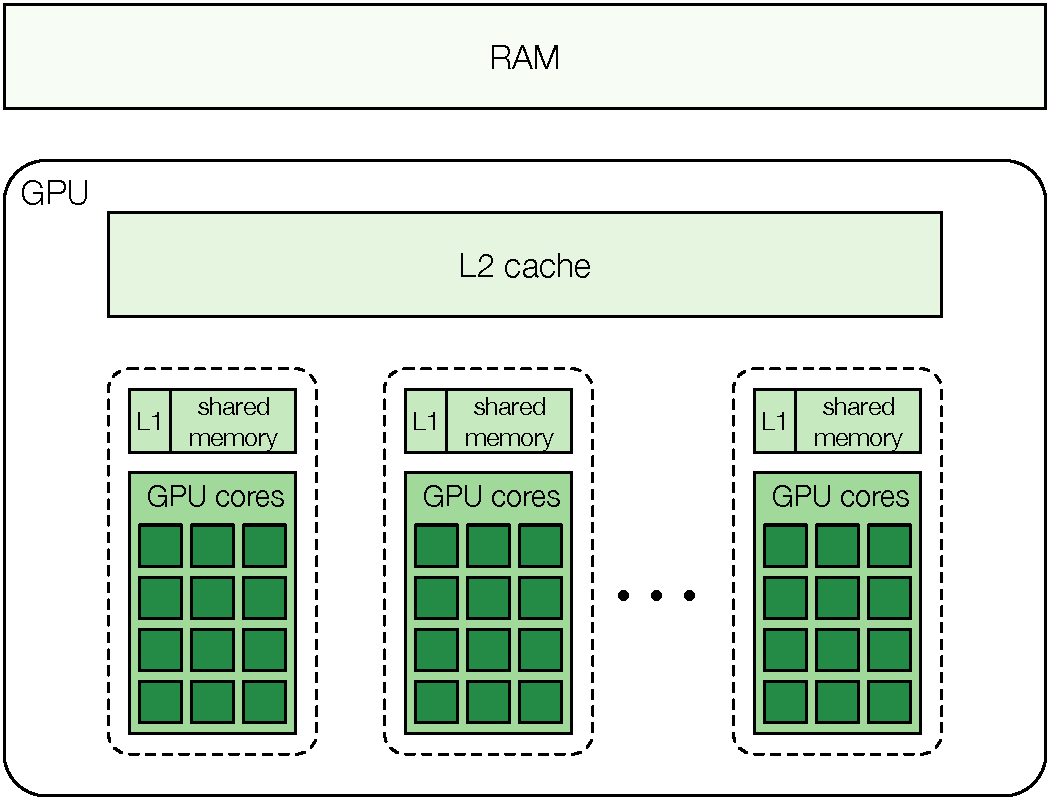
\includegraphics[width=.75\textwidth]{GPU}
  \caption{GPU architecture}
  \label{fig:gpu}
\end{figure}
% describe cores and execution
While the overall design looks fairly similar to the design of the multi-core \CPU, the architecture of the \GPU is actually very different in its details.
The lightweight \GPU cores are grouped together into what Nvidia calls a \emph{Streaming Multiprocessor} (SM).
In the Kepler architecture, an SM features 192 single-precision cores, 64 double-precision units, 32 special function units, and 32 memory units.
% \autoref{fig:gpuSM} shows the design of an SM in the Kepler architecture.
The 192 single-precision cores are very lightweight compared to the complex \CPU cores we discussed in the previous subsection.
A single \GPU core does not support SIMD vectorization:
it performs the straightforward in-order execution, and does not perform complex branch prediction.
This design makes the implementation of such a core in hardware cheap and enables the grouping of hundreds of cores in a single SM.

% describe caches and memory
Modern \GPUs feature two levels of caches:
the first level (L1) is private to each SM and the second level cache (L2) is shared among all SMs.
Compared to the cache sizes of the \CPU, the caches on the \GPU are fairly small.
The Kepler architecture features an L1 cache of 48 kilobyte and an L2 cache of 1.5 megabyte.
It is important to notice that these caches are shared by a vast amount of threads being executed on the \GPU:
the 48 kilobyte L1 caches are shared among up to 2048 threads being executed on a particular SM and the L2 cache is shared among up to about 30,\,000 threads.

Besides caches, each SM on a \GPU features also a scratchpad memory, called \emph{shared memory} in Nvidia's \GPU architectures.
This memory is small (16 or 48 kilobytes) but very fast as compared to the L1 cache.
While the L1 cache is automatically managed by a cache controller, the shared memory is explicitly managed by the programmer.

% make conclusions: throughput oriented => cores and threads important, different trade off: poor performance for single thread very good performance for data parallel applications => bad when: a lot of branching, less caches => memory accesses are expensive (coalescing ...)
The design of \GPUs is motivated by the overall goal to deliver maximal throughput even if this requires to sacrifice the performance of single threads~\cite{GarlandK10}.
This is why the \GPU cores are lightweight offering poor sequential performance, but thousands of cores combined together offer a very high computational throughput.
Memory latencies are mitigated by a high oversubscription of threads:
in the Kepler architecture an SM can manage up to 2048 threads which can be scheduled for execution on the 192 cores.
If a thread is waiting for a memory request, another thread continues its execution.
This is the reason why caches are fairly small, as they play a less important role as in \CPU architectures.

\paragraph{GPU Thread Execution}
The execution of threads on a \GPU is very different as compared to the execution on a traditional multi-core \CPU:
multiple threads are grouped by the hardware and executed together.
Such a group of threads is called a \emph{warp} by Nvidia.
In the Kepler architecture, 32 threads form a warp and an SM selects 4 warps and for each warp 2 independent instructions are selected to be executed in parallel on its single-precision cores, double-precision units, special function units, and memory units.

All threads grouped into a warp perform the same instructions in a lockstep manner.
Is is possible that two or more threads follow different execution paths.
In this case, all threads sharing a common execution path execute together while the other threads pause their execution.
It is beneficial to avoid warps with divergent execution paths, as this reduces or eliminates the amount of threads pausing their execution.
Nvidia calls this execution model: single-instruction, multiple-thread (SIMT).

Programmers are advised to manually optimize their code, so that all threads in a warp follow the same execution path.
Threads in the same warp taking different branches in the code can substantially hurt the performance and should, therefore, be avoided.

\paragraph{GPU Memory Accesses}
Accessing the main memory of a \GPU, called \emph{global memory}, is an expensive operation.
The \GPU can optimize accesses when the global memory is accessed in certain fixed patterns.
If the threads organized in a warp access a contiguous area of the memory, the hardware can \emph{coalesce} the memory access, \ie, perform a single memory request instead of issuing individual requests for every thread.
Several similar access patterns exist which are detected by the hardware to coalesce the memory accesses by multiple threads.

This is a major optimization opportunity for many \GPU programs, as the available memory bandwidth can only be utilized properly if memory accesses are coalesced.
Uncoalesced memory accesses may severely hurt the performance.


\paragraph{GPU Shared Memory}
% shared memory
The usage of the shared memory featured in each SM can substantially increase performance -- when used properly.
The programmer is responsible for exploiting this memory by explicitly moving data between the global memory and the shared memory.
All threads executing on the same SM have shared access to the shared memory at a high bandwidth and with low latency.
When multiple threads need to access the same data item, it is often beneficial to first load the data item into the shared memory by a single thread and perform all successive accesses on the shared memory.
This is similar to a cache with the difference that the programmer has to explicitly control its behavior.
Shared memory can also be used by a thread to efficiently synchronize and communicate with other threads running on the same SM.
On current \GPUs, global synchronization between threads running on different SMs is not possible.
% it is only possible for threads running on the same SM to synchronize, because global synchronization between threads running on different SMs is not possible.

\bigskip
Summarizing, current \GPU architectures are more sensitive to optimizations than \CPU architectures.
The most important optimizations on \GPUs are:
exploit the available parallelism by launching the right amount of threads, ensure that accesses to the global memory are coalesced, use the shared memory to minimize accesses to the global memory, and avoid divergent branches for threads organized in a warp~\cite{CUDATuningKepler2015}.

In addition to these optimizations, it is important for the programmer to keep in mind that the application exploiting the \GPU is still executed on the \CPU and typically only offloads computation-intensive tasks to the \GPU.
An often crucial optimization is to minimize the data transfer between the \CPU and the \GPU or overlap this transfer with computations on the \GPU.

\bigskip

\noindent
We now discuss the current approaches to program multi-core \CPUs and \GPUs in detail.



\section{Programming of Multi-Core CPUs and GPUs}
Arguably the most popular concept of parallel software for multi-core \CPUs is \emph{multithreading}.
Threading libraries exist for almost all popular programming languages, including C~\cite{Cstandard,Pthreads} and \Cpp~\cite{Cppstandard}.
Threads are conceptionally similar to processes in an operating system, with the major difference that threads share the same address space in memory while processes usually do not.
This enables threads to communicate and cooperate efficiently with each other by directly using the same memory.
Programmers have great flexibility and control over the exact behavior of the threads and their interaction, including the important questions of when and how many threads to use, how tasks and data are divided across threads, and how threads synchronize and communicate with each other.
The disadvantage of this high flexibility is that the burden of developing a correct and efficient program lies almost entirely on the programmer.
The interaction of threads executing concurrently can be very complex to understand and reason about, and traditional debugging techniques are often not sufficient as the execution is not deterministic any more.

\OpenMP~\cite{OpenMP} is a popular alternative approach focusing on exploiting parallelism of loops in sequential programs.
The focus on loops is based on the observation that loops often iterate over large data sets performing operations on every data item without any dependencies between iterations.
Such workloads are traditionally called \emph{embarrassingly parallel} and can be parallelized in a straightforward manner.
In \OpenMP, the programmer annotates such loops with compiler directives, and a compiler supporting the \OpenMP standard automatically generates code for performing the computations of the loop in parallel.
Recent versions of the \OpenMP standard and the closely related \OpenACC~\cite{OpenACC} standard support execution on \GPUs as well.
Here the programmer has to additionally specify the data regions which should be copied to and from the \GPU prior to and after the computation.
\OpenMP and \OpenACC allow for a fairly easy transition from sequential code to parallel code exploiting multi-core \CPUs and \GPUs.
Performance is often not optimal as current compilers are not powerful enough to apply important optimizations like cache optimizations, ensuring coalesced memory accesses, and the usage of the local memory.

\CUDA~\cite{CUDAProgrammingGuide} and \OpenCL~\cite{OpenCL} are the most popular approaches to program \GPU systems.
While \CUDA can only be used for programming \GPUs manufactured by Nvidia, \OpenCL is a standard for programming \GPUs, multi-core \CPUs, and other types of parallel processors regardless of their hardware vendor.
All major processor manufactures support the \OpenCL standard, including AMD, ARM, IBM, Intel, and Nvidia.
\CUDA and \OpenCL are similar programming approaches.
We will study the \OpenCL programming approach in more detail, as it is the technical foundation of the work presented later in \autoref{part:skelcl} and \autoref{part:codeGeneration} of this thesis.


\subsection{The OpenCL Programming Approach}
\OpenCL is a standard for programming multi-core \CPUs, \GPUs, and other types of parallel processors.
\OpenCL was created in 2008 and has since been refined multiple times.
In this thesis, we will use the \OpenCL standard version 1.1 which was ratified in June 2010.
This is the most commonly supported version of the standard with support from all major hardware vendors: AMD, ARM, Intel, and Nvidia.
The newer \OpenCL standards version 2.0 and 2.1 are currently not supported on Nvidia \GPUs.

\OpenCL is defined in terms of four theoretical models: platform model, memory model, execution model, and programming model.
We will briefly discuss all four models.

\paragraph{The \OpenCL Platform Model}
\autoref{fig:opencl} shows the \OpenCL platform model.
\OpenCL distinguishes between a \emph{host} and multiple \OpenCL \emph{devices} to which the host is connected.
In a system comprising of a multi-core \CPU and a \GPU, the \GPU constitutes an \OpenCL device and the multi-core \CPU plays the dual rule of the host and an \OpenCL device as well.
An \OpenCL application executes sequentially on the host and offloads parallel computations to the \OpenCL devices.

\OpenCL specifies that each device is divided into one or more \emph{compute units} (CU) which are again divided into one or more \emph{processing elements} (PE).
When we compare this to our discussion of multi-core \CPUs, there is a clear relationship:
a \CPU core corresponds to a compute unit and the functional units inside of the \CPU core performing the computations correspond to the processing elements.
For the \GPU the relationship is as follows:
a streaming multiprocessor corresponds to a compute unit and the lightweight \GPU cores correspond to the processing elements.

\begin{figure}
  \centering
  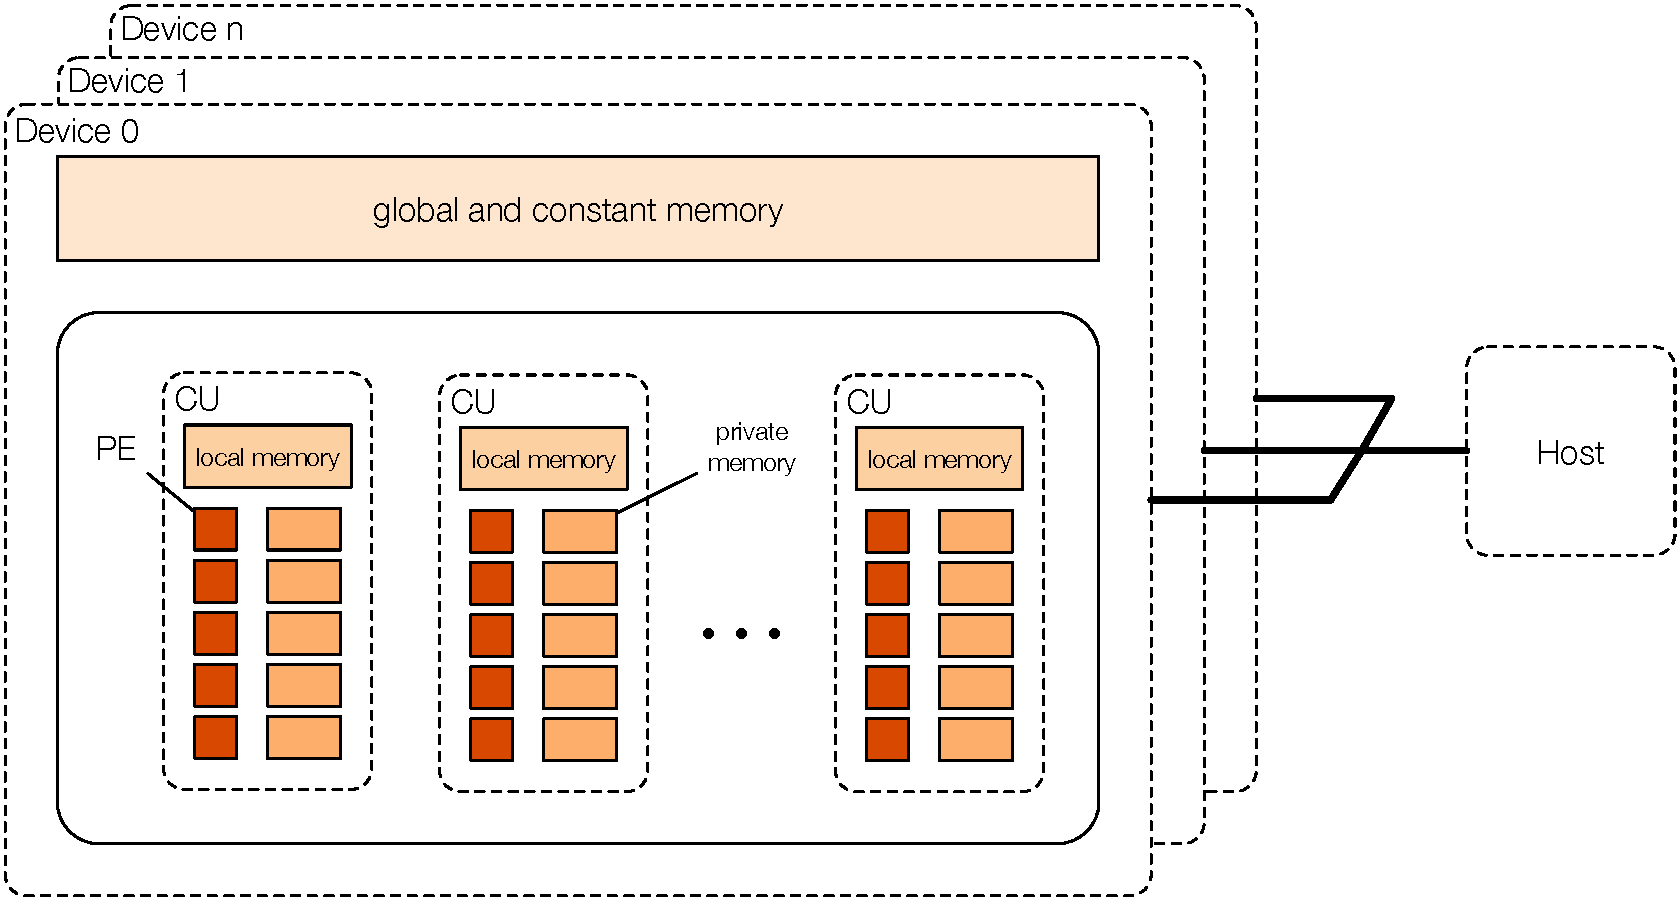
\includegraphics[width=.95\textwidth]{OpenCL}
  \caption{The \OpenCL Platform and Memory Model}
  \label{fig:opencl}
\end{figure}

\paragraph{The \OpenCL Memory Model}
Each device in \OpenCL has its own memory.
This memory is logically (but not necessarily physically) distinct from the memory on the host.
Data has to be moved explicitly between the host and device memory.
The programmer issues commands for copying data from the host to the device and vice versa.

On a device, \OpenCL distinguishes four memory regions:
global memory, constant memory, local memory, and private memory.
These memory regions are shown in \autoref{fig:opencl}.

The \emph{global memory} is shared by all compute units of the device and permits read and write modifications from the host and device.
% Dynamic memory allocations are possible from the host, but there is no possibility to allocate global memory from the device side.
The global memory is usually the biggest but slowest memory area on an \OpenCL device.

The \emph{constant memory} is a region of the global memory which remains constant during device execution.
% The host can dynamically allocate regions of the constant memory and can read and write to it.
% The device can statically allocate constant memory and only read from it.
The host can read and write to the constant memory, but the device can only read from it.

The \emph{local memory} is a memory region private to a compute unit.
It permits read and write accesses from the device; the host has no access to tis memory region.
% Memory can either be allocated dynamically from the host or statically from the device.
The local memory directly corresponds to the fast per-SM shared memory of modern \GPUs.
On multi-core \CPUs, the local memory is usually only a logical distinction:
local memory is mapped to the same physical memory as the global memory.

The \emph{private memory} is a memory region private to a processing element.
The device has full read and write access to it, but the host has no access at all.
The private memory contains all variables which are private to a single thread.


\paragraph{The \OpenCL Execution Model}
The communication between the host and a particular device is performed using a \emph{command queue}.
The host submits commands into a \emph{command queue} which by-default processes all commands in the first-in-first-out order.
It is also possible to configure command queues to operate out-of-order, \ie, no order of execution of commands is guaranteed.

There exist three types of commands which can be enqueued in a command queue.
A \emph{memory command} indicates to copy data from the host to the device or from the device to the host.
A \emph{synchronization command} enforces a certain order of execution of commands.
Finally, a \emph{kernel execution command} executes a computation on the device.

A \emph{kernel} is a function which is executed in parallel on an \OpenCL device.
\autoref{lst:openclExample} shows a simple \OpenCL kernel performing matrix multiplication.
When launching a kernel on a device, the programmer explicitly specifies how many threads will execute in parallel on the device.
A thread executing a kernel is called a \emph{work-item} in \OpenCL.
Work-items are grouped together in \emph{work-groups} which allow a more coarse-grained organization of the execution.
All work-items of a work-group share the same local memory, and synchronization between work-items of the same work-group is possible but it is forbidden for work-items from different work-groups.
This is because all work-items from the same work-group are guaranteed to be executed on the same CU, but this guarantee does not hold for work-items from different work-groups.

\begin{lstlisting}[float, caption={Example of an \OpenCL kernel.}, label={lst:openclExample}]
kernel void matMultKernel(global float* a, global float* b,$\label{lst:openclExample:1}$
                          global float* c, int width) {$\label{lst:openclExample:2}$
 int colId = get_global_id(0); int rowId = get_global_id(1);$\label{lst:openclExample:3}$

 float sum = 0.0f;
 for (int i = 0; i < width; ++i)
   sum += a[rowId * width + k] * b[k * width + colId];

 c[rowId * width + colId] = sum;
}
\end{lstlisting}

\OpenCL kernels are implemented in a dialect of C (starting with \OpenCL 2.1 a dialect of \Cpp) with certain restrictions as well as extensions.
The most prominent restrictions are:
recursive functions and function pointers are not supported, as well as system calls, including \code{malloc}, \code{printf}, file I/O, etc.
The most important extensions are:
qualifiers for pointers reflecting the four address spaces (\eg, the \code{global} qualifier in \autoref{lst:openclExample:1} and \autoref{lst:openclExample:2} of \autoref{lst:openclExample}) and vector data types, like \code{float4}.
Moreover, \OpenCL provides a set of functions which can be used to identify the executing work-item and work-group.
One example is the \code{get\_global\_id} function used in \autoref{lst:openclExample:3} of \autoref{lst:openclExample}.
This is usually used so that different work-items operate on different sets of the input data.
In \autoref{lst:openclExample}, each work-item computes one item of the result matrix \code{c} by multiplying and summing up a row and column of the input matrices \code{a} and \code{b}.
This kernel only produces the correct result if exactly one work-item per element of the result matrix is launched.
If the host program launches a different configuration of work-items then only part of the computation will be performed or out-of-bound memory accesses will occur.

\paragraph{The \OpenCL Programming Model}

\OpenCL supports two programming models: data parallel programming and task parallel programming.
The predominant programming model for \OpenCL is the data parallel programming model.

In the \emph{data parallel programming model}, kernel are executed by many work-items organized in multiple work-groups.
Parallelism is mainly exploited by the work-items executing a single kernel in parallel.
This programming model is well suited for exploiting modern \GPUs and, therefore, widely used.
This model is also well suited for modern multi-core \CPUs.

In the \emph{task parallel programming model}, kernels are executed by a single work-item.
Programmers exploit parallelism by launching multiple tasks which are possibly executed concurrently on an \OpenCL device.
This programming model is not well suited for exploiting the capabilities of modern \GPUs and, therefore, not widely used.

\section{Structured Parallel Programming}
% structured parallel programming & functional foundations
\emph{Structured programming} emerged in the 1960s and 1970s as a reaction to the ``software crises''.
Back then (and still today) programs were often poorly designed, hard to maintain, and complicated to reason about.
Dijkstra identified the low-level \code{goto} statement as a major reason for programmers writing ``spaghetti code''.
In the famous letter~\cite{Dijkstra68a}, he argued that programs should organize code more structurally in procedures and using higher-level control structures like \code{if} and \code{while}.
Dijkstra's letter helped to eventually overcome unstructured sequentiell programming and to establish structured programming~\cite{DahlDiHo1972}.
The new structures proposed to replace \code{goto} where suggested based on observations of common use cases -- or \emph{patterns} of use -- of the \code{goto} statement in sequential programming.
By capturing an entire pattern of usage, these patterns raise the abstraction level and make it easier to reason about them.
An \code{if A then B else C} statement has a clear semantic which is easy to understand and reason about, for example is it clear to the programmer -- and the compiler -- that \code{B} and \code{C} cannot both be executed.
This helps the programmer to understand the source code and the compiler to produce an optimized executable.
The equivalent unstructured code containing multiple \code{goto} statements obtains the same high-level semantic by combining the low-level operations with their low-level semantics.
Both, programmer and compiler, have to ``figure out'' the high-level semantic by means of analyzing the sequence of low-level operations and reconstructing the overall semantic.

In recent years researchers have suggested similar arguments to Dijkstra's for addressing the challenges attached with traditional parallel programming by introducing \emph{structured parallel programing}.
For parallel programming using message passing, Gorlatch argues similar to Dijkstra that single send and receive statements should be avoided and replaced by collective operations~\cite{Gorlatch04}.
Each collective operation, \eg, broadcast, scatter, or reduce, captures a certain common communication pattern traditionally implemented with individual send and receive statements.
In~\cite{McCoolRoRe2012}, the authors argue that \emph{structured parallel patterns}, each capturing a common computation and communication behavior, should be used to replace explicit thread programming to improve the maintainability of software.
The book discusses a set of parallel patterns and their implementation in different recent programming approaches.
The underlying ideas go far back to the 1980s when Cole was the first to introduced \emph{algorithmic skeletons} to structure and, therefore, simplify parallel programs~\cite{Cole1991}.
As with sequential structured programming, structured parallel programming raises the abstraction level by providing high-level constructs: collective operations, parallel patterns, or algorithmic skeletons.
The higher level of abstraction both simplifies the reasoning about the code for the programmer and enables higher-level optimizations performed by the compiler.

As our work directly extends the ideas of Cole, we will discuss algorithmic skeletons in more detail next.

\subsection{Algorithmic Skeletons}
Cole introduced algorithmic skeletons as special higher-order functions which describe the ``computational skeleton'' of a parallel algorithm.
Higher-order functions are a well-known concept in functional programming and describe functions accepting other functions as arguments or returning a function as result.
This is often useful, as it allows to write more abstract and generic functions.

An example for an algorithmic skeletons is the \emph{divide \& conquer skeleton} which was among the original suggested skeletons by Cole~\cite{Cole1991}:
\begin{align*}
  D_C\ indivisible\ split\ join\ f% &= F\\
%  \textit{where}\ F\ P &= f\ P, \textit{ if  } indivisible\ P\nonumber\\
%                     &= join\ (map\ F\ (split\ P)), \textit{ otherwise}\nonumber
\end{align*}
The algorithmic skeleton $D_C$ accepts four functions as its arguments:
\begin{itemize}
  \item $indivisible$ is a function deciding if the given problem should be decomposed (divided) or not,
  \item $split$ is a function decomposing a given problem into multiple sub-problems,
  \item $join$ is a function combining multiple solved sub-problems into a larger solution,
  \item $f$ is a function solving an indivisible problem, \ie, the base case.
\end{itemize}

Applications like the discrete Fourier transformation, approximate integration, or matrix multiplication can be expressed and implemented using this algorithmic skeleton.
The application developer provides implementations for the functions required by the algorithmic skeleton to obtain a program which can be applied to the input data.

An algorithmic skeleton has a parallel implementation.
In the example of the $D_C$ skeleton, the implementation follows the well-known divide \& conquer technique which divides problems into multiple sub-problems which can be solved independently in parallel.
The implementation of the algorithmic skeleton hides the complexities of parallelism from the user.
It, therefore, provides a higher-level interface abstracting away the details of the parallel execution, including low-level details like launching multiple threads, as well as synchronization and communication of threads.

\paragraph{A Classification of Algorithmic Skeletons}
Algorithmic skeletons can broadly be classified into three distinct classes~\cite{Gonzalez-VelezL10}:
\begin{itemize}
  \item \emph{data-parallel skeletons} transform typically large amounts of data,
  \item \emph{task-parallel skeletons} operate on distinct tasks which potentially interact with each other,
  \item \emph{resolution skeletons} capture a family of related problems.
\end{itemize}

Examples of data-parallel skeletons are \emph{map} which applies a given function to each element of its input data in parallel, or \emph{reduce} which performs a parallel reduction based on a given binary operator.
Well known task-parallel skeletons are \emph{farm (\aka, master-worker)} where independent tasks are scheduled for parallel execution by the workers, or \emph{pipeline} where multiple stages are connected sequentially and the execution of all stages can overlap to exploit parallelism.
Finally, the discussed $D_C$ skeleton is an example of a resolution skeleton which captures the family of problems which can be solved by applying the divide \& conquer technique.

In this thesis, we will mainly focus on data-parallel skeletons, as they are especially suitable for the data-parallel \GPU architecture.
We will also introduce two new resolution skeletons which capture two specific application domains for which we can provide efficient \GPU implementations as well.

\subsection{Advantages of Structured Parallel Programming}
Structured parallel programming offers various advantages over the traditional unstructured parallel programming.

\bigskip

\paragraph{Simplicity}
Structured parallel programming raises the level of abstraction by providing higher-level constructs which serve as basic building blocks for the programmer.
Lower-level details are hidden from the programmer and handled internally by the implementation of the algorithmic skeletons.
This simplifies the reasoning about programs and helps in the development process, as well as increases the maintainability of the software.

\paragraph{Safety and Determinism}
Potentially dangerous low-level operations are not used directly by the programmer in structured parallel programming.
Therefore, issues like deadlocks and race conditions can be entirely avoided -- given a correct and safe implementation of the provided algorithmic skeletons.
Furthermore, the high-level semantic of the algorithmic skeletons can guarantee determinism, while the lacking of determinism due to the parallel execution is a major concern in low-level, unstructured parallel programming; this concern complicates development and debugging of the software.

\paragraph{Portability}
% portability of functionality
Algorithmic skeletons offer a single high-level interface but can be implemented in various ways on different hardware systems.
Existing skeleton libraries target distributed systems~\cite{Kuchen02,AldinucciCDKT12,MatsuzakiKIHA04}, shared memory systems like multi-core \CPUs~\cite{AldinucciDaKiTo2011,CiechanowiczK10,LeytonP10}, and -- as we will discuss in this thesis -- systems with multiple \GPUs as well.
In contrary, unstructured parallel programming commits to a low-level programming approach targeting a particular hardware architecture, thus, making portability a major issue.
Furthermore, algorithmic skeletons evolved from functional programming and are, therefore, by-nature composabel and offer a high degree of re-use.

% performance portability
Another issue of portability is the portability of performance:
can a certain level of performance be obtained when switching from one hardware architecture to another?
This is virtually absent from low-level unstructured parallel programming as programmers apply low-level hardware-specific optimizations to achieve high performance.
These optimizations are usually not portable, as we will show later in \autoref{chapter:codeGeneration}.
Performance portability is a challenging and timely research topic which we address in this thesis by introducing a novel approach using structured parallel programming to achieve performance portability.

\pagebreak
\paragraph{Predictability}
The structure and regularity of structured parallel programming allows to build performance models which can be used in the development process to estimate the performance of the developed software.
Many research projects are devoted to this topic, showing that it is possible to predict the runtime of programs expressed with algorithmic skeletons~\cite{HayashiC02,DarlingtonFHKSW93,BischofGK03,Alt2007,StegmeierFrJAUn2015}.
Examples for related work in this area include work on particular algorithmic skeletons~\cite{BischofGK03}, work targeted towards distributed and grid systems~\cite{Alt2007}, and recently work targeting real-time systems~\cite{StegmeierFrJAUn2015}.

\paragraph{Performance and Optimizations}
Many studies have shown that structured parallel programs can offer the same level of performance as programs implemented and optimized with traditional unstructured techniques.
Examples include application studies on grid systems~\cite{Alt2007}, distributed systems~\cite{CiechanowiczKSGK09}, as well as systems featuring multi-core \CPUs~\cite{AldinucciMT10}.
In this thesis, we will investigate the performance of programs expressed with data-parallel algorithmic skeletons on systems with one or multiple \GPUs.

The high-level semantic of algorithmic skeletons enable high-level optimizations like the rewrite rules presented in~\cite{Gorlatch00}.
These optimizations exploit information about the algorithmic structure of a program which is often hard or impossible to extract from unstructured programs.
In this thesis, we will present a system for encoding and systematically applying such high-level optimizations to generate highly optimized code from a high-level, skeleton-based program representation.


%\from{HIPS begin}
%\section{GPU programming using OpenCL (HIPS)}
%
%The OpenCL standard~\cite{OpenCL} can be used for programming any OpenCL-capable device.
%These devices embrace most modern GPUs and other accelerators, e.\,g., the Cell BE, as well as standard multi-core CPUs.
%
%OpenCL distinguishes between a \emph{host} system, usually containing one or several CPUs, and \emph{devices} that are integrated into the host system.
%An OpenCL device logically consists of one or more \emph{compute units} (CUs) that are divided into one or more \emph{processing elements} (PEs).
%All computation on the device is performed in the PEs.
%OpenCL applications run on the host and call \emph{kernel functions} which are executed simultaneously by multiple PEs on one or more devices.
%A single instance of a kernel function is called a \emph{work-item} and can be identified by its \emph{global ID}.
%Every work-item executes the same code, but the execution can vary per work-item due to branching according to the global ID.
%Work-items are organized in \emph{work-groups}.
%When a kernel function is started, the host code specifies how many work-items are launched and how many work-items form a work-group.
%All work-items in one work-group are executed on the same CU.
%Therefore, the size of a work-group can have a significant effect on the runtime performance.
%
%In OpenCL, host and device have separate memories.
%Thus, functions are provided to transfer data from the host's to the device's memory (\emph{upload}) and back (\emph{download}).
%Memory areas have to be allocated on the device before data can be accessed by it and deallocated thereafter.
%
%For portability across a wide range of devices, kernel functions are compiled at runtime.
%The host program passes the kernel's source code as a plain string to the OpenCL driver to create executable binary code.
%This is different compared to CUDA which provides a special compiler \texttt{nvcc} to compile the device code and the host code.
%
%Creating applications for multi-GPU systems introduces new challenges, like partitioning the application appropriately and, explicitly implementing data transfer between devices~\cite{SchellmannVG08}.
%The host application must coordinate and perform synchronization and data exchange explicitly.
%The source code for performing such exchanges further increases the amount of boilerplate code.
%
%In the following, we describe how our SkelCL library addresses these problems of GPGPU programming.
%\from{HIPS end}
%
%
%\from{HiStencils begin}
%\section{Stencils Using OpenCL (HiStencils)}
%\label{sec:background}
%
%A \emph{stencil computation} is a computation pattern on a multi-dimensional grid, where each point of the grid is updated (often iteratively) as a function of its neighboring points.
%Each point of the grid stores a set of application-dependent values.
%The computation performed to update the values of each point is called the \emph{stencil operation}.
%A stencil operation updates the value of a point depending on the values of the neighboring points.
%The points taken into account for a stencil operation are defined by the \emph{stencil shape}.
%
%Let us consider how stencil computations are implemented on manycore systems with GPUs using the state-of-the-art OpenCL standard.
%Listing~\ref{lst:sobel_opencl} presents the structure of an OpenCL implementation of the Sobel operator on one GPU, a typical stencil computation used in image processing for detecting edges in images.
%Lines 9--13 show how the direct neighboring elements, e.g., the \emph{upper left} (\texttt{ul}) neighbor, are accessed and passed to a function performing the Sobel operation in line 16.
%Many low-level details have to be considered for a correct implementation, like raw pointer handling, including index computations (e.g., line 10), and explicit out-of-bound  accesses handling (e.g., line 9).
%
%\begin{lstlisting}[%
%caption={Structure of the OpenCL implementation of Sobel edge detection},%
%float=tbp,%
%label={lst:sobel_opencl}]
%kernel
%  void sobel(global const char* in_img,
%             global char* out_img,
%             int w, int h) {
%  int i = get_global_id(0);
%  int j = get_global_id(1);
%
%  if (i < w && j < h) {
%    char ul = (j-1 > 0 && i-1 > 0)
%        ? in_img[((j-1)*w)+(i-1)] : 0;
%    ...
%    char lr = (j+1 < h && i+1 < w)
%        ? in_img[((j+1)*w)+(i+1)] : 0;
%
%    out_img[j*w+i] =
%        computeSobel(ul, ..., lr);
%  }
%}
%\end{lstlisting}
%
%The OpenCL version is obviously correct, but not efficient:
%the fast local GPU memory is not used and the control flow diverges heavily between different work items, which is disadvantageous on current GPU architectures.
%However, the corresponding optimizations require a deep knowledge of the GPU's architecture and must be programmed and tuned manually and are, therefore, a complicated task for application developers.
%If the program is to be used on a multi-GPU system then the application developer has to additionally implement and optimize the explicit data distribution across GPUs and the communication between them.
%\from{HiStencils end}
%
%\from{PACT begin}
%\section{OpenCL (PACT)}
%\paragraph{OpenCL Execution Model}
%OpenCL can be used to program manycore CPUs and GPUs.
%Both are typically represented in the system as an accelerator.
%Programming these devices consists of writing a compute \emph{kernel} in OpenCL C that executes on the device and writing the host code that orchestrates data movement, allocates memory and manages the execution on the device.
%
%\paragraph{Thread Organization and Synchronization}
%Most GPUs are organized as multicore processors with each core executing multiple threads concurrently.
%OpenCL represents this with the concept of \emph{workgroups} that contain \emph{local threads}.
%Threads within a core are typically grouped in \emph{warps} (using Nvidia terminology) where each thread executes in a lock-step synchronized manner.
%Only one warp is active at a time and execution switches to a different warp when the pipeline stalls to hide memory latency.
%OpenCL allows to synchronize threads at the kernel level on the host or at the workgroup level using a barrier function synchronizing the local threads.
%Threads within a warp are implicitly synchronized on GPUs.
%
%
%\paragraph{Vector Units}
%Most modern CPUs and devices such as AMD GPUs integrates vector units that can process more than on data element at a time.
%The OpenCL programming model exposes this with special data types such as \texttt{int4} where any operations on this type will be executed in the vector units.
%In the absence of vector units in the hardware, the OpenCL compiler scalarizes the code automatically.
%
%\paragraph{Memory Coalescing}
%On GPUs, requests to the main device memory are usually performed at the granularity of a cache line, which is typically 64 bytes.
%Therefore, due to the organization of the threads in warps, it is important to ensure that consecutive threads access consecutive memory elements to maximize memory bandwidth.
%
%\paragraph{Local Memory}
%Most GPUs have a per-core cache and a local memory shared among all local threads.
%OpenCL defines a global and local address space.
%On GPUs, local memory has a high bandwidth and low latency and is used to store frequently accessed data.
%On CPUs, local memory is usually simply mapped to a region of global memory.
%\from{PACT end}

% include related work
%\section{Related work}

\from{HIPS begin}
\subsection{HIPS}
% ------------------------------------------------------------------------------

There are a number of other projects aiming at high-level GPU programming.

\emph{SkePU}~\cite{EnmyrenKe10} uses container classes and algorithmic skeletons to ease multi-GPU computing.
Although SkePU and SkelCL have been developed independently, both projects share some concepts:
SkePU provides a vector class similar to SkelCL's \texttt{Vector} class, but unlike SkelCL it does not support different kinds of data distribution on multi-GPU systems.
SkePU and SkelCL both provide a map and a reduce skeleton.
However, SkelCL additionally provides the \texttt{Zip} and \texttt{Scan} skeleton, while SkePU supports two additional variants of the map skeleton.
Unlike SkelCL, which allows for an arbitrary number of arguments, in SkePU the user-defined functions are restricted to a fixed skeleton-specific number of arguments.
Currently, SkePU is the only project other than SkelCL that supports data-parallel computations on multi-GPU systems.
SkelCL provides a more flexible memory management than SkePU, as data transfers can be expressed by changing data distribution settings.
Only this flexibility provides the best performance for our second case study (Section~\ref{sec:list-mode_OSEM}) and similar applications.
Both projects differ significantly in the way how functions are passed to skeletons.
While functions are defined as plain strings in SkelCL, SkePU uses a macro language, which brings some serious drawbacks.
For example, it is not possible to call mathematical functions like sin or cos inside a function generated by a SkelPU macro,
because these functions are either named differently in all three target programming models or might even be missing entirely.
The same holds for functions and keywords related to performance tuning, e.\,g., the use of local memory.
SkelCL does not suffer from these drawbacks because it relies on OpenCL and thus can be executed on a variety of devices.

\emph{CUDPP}~\cite{SenguptaHZO07} is a C++ library based on CUDA.
It provides data-parallel algorithm primitives similar to skeletons.
These primitives can be configured using only a predefined set of operations, whereas
skeletons in SkelCL are true higher-order functions, which accept any user-defined function.
CUDPP does not simplify data management, because data still has to be exchanged between CPU and GPU explicitly.
There is also no support for multi-GPU applications.

\emph{Thrust}~\cite{BellHo2011} is an open-source library by NVIDIA.
It provides two vector types similar to the vector type of the C++ Standard Template Library.
While these types refer to vectors stored in CPU or GPU memory, respectively, SkelCL's vector data type provides a unified abstraction for CPU and GPU memory.
Thrust also contains data-parallel implementations of higher-order functions, similiar to SkelCL's skeletons.
SkelCL adopts several of Thrust's ideas, but it is not limited to CUDA-capable devices and supports multiple GPUs.

Unlike SkelCL, \emph{PGI Acccelerator}~\cite{PGI-10} and \emph{HMPP}~\cite{HMPP-09} are compiler-based approaches to GPU programming, similar to the popular OpenMP~\cite{OpenMP-08}.
The programmer uses compiler directives to mark regions of code to be executed on a GPU.
A compiler generates executable code for the GPU, based on the used directives.
Although source code for low-level details like memory allocation or data exchange is generated by the compiler, these operations still have to be specified explicitly by the programmer using suitable compiler directives.
We consider these approaches low-level, as they do not perform data transfer automatically to shield the programmer from low-level details.
\from{HIPS end}

\from{ASHES begin}
\subsection{ASHES}
SkelCL is a runtime, library-based approach for GPU programming, unlike compiler-based approaches, e.\,g., \emph{HMPP}~\cite{HMPP-07} and the \emph{PGI Accelerator compilers}~\cite{PGI-10}.
It offers the user a consistent high-level API while still allowing the programmer to use all features of the underlying OpenCL standard.

There are other library-based approaches for high-level GPU programming.

\emph{SkePU}~\cite{EnmyrenKe10} is a skeleton-based framework for multi-core CPUs and multi-GPU systems.
An architecture-independent macro language is used which, however, makes architecture-specific optimizations impossible, like the use of local memory in OpenCL.
SkelCL avoids this drawback by building on top of OpenCL.
SkePU provides memory abstractions similar to SkelCL, but does not support different data distributions on multi-GPU systems as in SkelCL:
vectors are always distributed to all available devices, with no possibility of data exchanges between devices.
Therefore, our list-mode OSEM application which heavily relies on multiple data exchanges between devices cannot be implemented efficiently using SkePU.

\emph{Thrust}~\cite{BellHo2011} provides an interface similar to the C++ Standard Template Library (STL).
For data management, two distinct dynamic containers, a \texttt{host\_vector} and a \texttt{device\_vector}, can be used like STL vectors for managing host and device memory respectively.
% Data is copied to a device by assigning a \texttt{host\_vector} to a \texttt{device\_vector}.
In addition, Thrust offers common parallel algorithms, including searching, sorting, reductions, and transformations.
Thrust is based on CUDA, therefore, restricting the user to NVIDIA GPUs.

\emph{GPUSs}~\cite{AyBILMQ-09} is an implementation of the Star Superscalar model for multi-GPU systems.
While SkelCL is focused on data parallelism, GPUSs provides simple task parallelism;
annotations are used for data transfers between host and GPU.
SkelCL offers a higher level of memory abstraction: communication is specified implicitly by a distribution scheme instead of individual data transfers.

Rabhi and Gorlatch~\cite{RaG-03} present different approaches of skeletal programming for parallel as well as distributed systems.
Gonz\'{a}lez-V\'{e}lez and Leyton~\cite{GoL-10} provide an overview of available skeleton frameworks.
\from{ASHES end}

\from{ICCS begin}
\subsection{ICCS}
A considerable amount of work exists in the filed of algorithmic skeletons;
for an overview we refer to~\cite{gc11}.
There are several related approaches to raise the level of program abstraction in GPU programming.
While SkelCL can be used for programming multiple OpenCL capable GPUs, the CUDA-based \emph{Thrust}~\cite{BellHo2011} library simplifies programming only for a single NVIDIA GPU.
As SkelCL, \emph{SkePU}~\cite{EnK-10} is a skeleton library targeting multi-GPU systems.
In contrast to our work which is based entirely on the portable OpenCL, SkePU is implemented with multiple back-ends which restrict the application developer to the back-ends' smallest common set of functions and, thus, prevents the user from applying optimizations, like using the fast local GPU memory.
\from{ICCS end}

\from{HLPP begin}
\subsection{HLPP}
Considerable theoretical as well as practical research has been conducted in the field of algorithmic skeletons since its introduction in the late 1980s.
Due to lack of space, we refer to~\cite{GoC-11} for an overview of skeletal programming and~\cite{gl10} for a recent survey of skeleton libraries for clusters and multi-core CPUs.
Our contribution to skeletal programming is the introduction and efficient implementation of a new algorithmic skeleton for performing allpairs computations.
As other skeletons, the allpairs skeleton can be used as a basic building block by application developers who do not have to be experts in GPU computing or parallel programming in general.

In previous work, efficient parallel implementations of allpairs computations on modern parallel processors were studied (e.\,g., multi-core CPUs~\cite{AroraShVu2009}, the Cell processor~\cite{WirawanSK09}, and GPUs~\cite{ChangDeQuRo2009}) in the context of specific applications.
In contrast to~\cite{SarjeAl2013}, which presents an efficient implementation scheme of allpairs computations for GPUs, we abstract the computation as an algorithmic skeleton and offer its efficient implementation to application developers as part of the SkelCL skeleton library.

The evaluation of the programming effort shows that the allpairs skeleton allows to express many applications considerably shorter and at a higher level of abstraction, as compared to using OpenCL or library implementations like BLAS.
The performance comparison shows that by making information about the memory access pattern available to the implementation, we can considerably improve the performance by efficiently using the fast GPU local memory.

Several current approaches address simplifying GPU programming.
As SkelCL, also SkePU~\cite{EnmyrenKe10} and Muesli~\cite{ErK-12} are skeleton libraries targeting multi-GPU systems.
In contrast to our work, which is based entirely on the portable OpenCL, Muesli is implemented using NVIDIA's CUDA and SkePU is implemented with multiple back-ends which restrict the application developer to the back-ends' smallest common set of functions.
While SkelCL can be used for programming multiple OpenCL-capable GPUs, the CUDA-based Thrust~\cite{BellHo2011} library simplifies programming only for a single NVIDIA GPU.
\from{HLPP end}

\from{PaCT begin}
\subsection{PaCT}
There are a number of other projects aiming at high-level GPU programming.

\emph{SkePU}~\cite{EnmyrenKe10} provides a vector class similar to our \texttt{Vector} class, but unlike SkelCL it does not support different kinds of data distribution on multi-GPU systems.
SkelCL provides a more flexible memory management than SkePU, as data transfers can be expressed by changing data distribution settings.
Both approaches differ significantly in the way how functions are passed to skeletons.
While functions are defined as plain strings in SkelCL, SkePU uses a macro language, which brings some serious drawbacks.
For example, it is not possible to call mathematical functions like sin or cos inside a function generated by a SkelPU macro,
because these functions are either named differently in all of their three target programming models (CUDA, OpenCL, OpenMP) or might even be missing entirely.
The same holds for functions and keywords related to performance tuning, e.\,g., the use of local memory.
SkelCL does not suffer from these drawbacks because it relies on OpenCL and thus can be executed on a variety of GPUs and other accelerators.

\emph{CUDPP}~\cite{SenguptaHZO07} provides data-parallel algorithm primitives similar to skeletons.
These primitives can be configured using only a predefined set of operations, whereas
skeletons in SkelCL are true higher-order functions which accept any user-defined function.
CUDPP does not simplify data management, because data still has to be exchanged between CPU and GPU explicitly.
There is also no support for multi-GPU applications.

\emph{Thrust}~\cite{BellHo2011} provides two vector types similar to the vector type of the C++ Standard Template Library.
While these types refer to vectors stored in CPU or GPU memory, respectively, SkelCL's vector data type provides a unified abstraction for CPU and GPU memory.
Thrust also contains data-parallel implementations of higher-order functions, similiar to SkelCL's skeletons.
SkelCL adopts several of Thrust's ideas, but it is not limited to CUDA-capable GPUs and supports multiple GPUs.

Unlike SkelCL, \emph{OpenACC}~\cite{OpenACC}, \emph{PGI Acccelerator}~\cite{PGI-10}, and \emph{HMPP}~\cite{HMPP-09} are compiler-based approaches to GPU programming, similar to the popular OpenMP~\cite{OpenMP-08}.
The programmer uses compiler directives to mark regions of code to be executed on a GPU.
A compiler generates executable code for the GPU, based on the used directives.
Although source code for low-level details like memory allocation or data exchange is generated by the compiler, these operations still have to be specified explicitly by the programmer using suitable compiler directives.
We consider these approaches low-level, as they do not perform data transfer automatically to shield the programmer from low-level details and parallelism is still expressed explicitly.
\from{PaCT end}

\from{HiStencils begin}
\subsection{HiStencils}
Several approaches aiming at simplifying GPU programming exist.
\emph{SkePU}~\cite{EnmyrenKe10} provides a vector class similar to our \texttt{Vector} class, but unlike SkelCL it does not support different kinds of data distribution on multi-GPU systems.
SkelCL provides a more flexible memory management than SkePU, as data transfers can be expressed by changing data distribution settings.
\emph{Thrust}~\cite{BellHo2011} provides two vector types similar to the vector type of the C++ Standard Template Library.
While these types refer to vectors stored in CPU or GPU memory, respectively, SkelCL's vector data type provides a unified abstraction for CPU and GPU memory.
Thrust also contains data-parallel implementations of higher-order functions, similiar to SkelCL's skeletons.
SkelCL adopts several of Thrust's ideas, but it is not limited to CUDA-capable GPUs and supports multiple GPUs.
Both SkePU and Thrust provide no explicit support for stencil computations.

Several projects focus on stencil computations on GPUs.
PATUS~\cite{PATUS} is a code generation and tuning framework for stencil computations.
It can generate optimized code for multicore processors and a single GPU.
PARTANS~\cite{PARTANS} is a code generation and autotuning framework for stencil computations on multiple GPUs. 
It automatically distributes and optimizes stencil computations on multiple GPUs, by searching for optimal parameters for a given hardware architecture.
These specialized domain-specific approaches can only be applied to stencil computations, whereas SkelCL is a general-purpose approach.
\from{HiStencils end}


\from{PACT begin}
\subsection{PACT}

\paragraph{Algorithmic Patterns}
Algorithmic patterns or skeletons~\cite{cole88skeleton} have been around for more than two decades.
The Map-Reduce~\cite{dean08mapreduce} framework from Google for instance allows programmers to express computation using two operators; map and reduce.
Since the original framework was developed, many researchers have looked at the problem of optimizing these operations for different type of hardware.
Paraprox~\cite{Samadi14Paraprox} for instance uses automatic detection of algorithmic patterns to apply optimization at the expense of accuracy.
Compared to our approach, most prior works rely on hardware-specific implementations to achieve high performance.
Conversely, we automatically generate implementations using our fine-grain hardware patterns combined with our rule rewriting system.

\paragraph{Functional Approaches for GPU Code generation}
Accelerate is a functional domain specific language built within Haskell to support GPU acceleration~\cite{chakravarty11accelerating,mcdonell13optimising}.
Recently, Nvidia has released technical reports on NOVA~\cite{collins13nova}, a new functional language target at code generation for GPUs, and Copperhead~\cite{catanzaro11copperhead}, a data parallel language embedded in Python.
Nova shares many concepts from Accelerate and Copperhead and offers familiar data parallel patterns.
HiDP~\cite{zhang13hidp} is a hierarchical data parallel language which maps computations to the OpenCL programming model similar to our approach.
All these projects rely on analysis of user code or hand-tuned versions of high-level algorithmic patterns.
In contrast, our approach uses rewrite rules and low-level hardware patterns to produce high-performance code in a portable way.

\paragraph{Rewrite-rules for Optimizations}
Rewrite rules have been used very early as a way to automate the optimization process of functional programs~\cite{jones01playing}.
Similar to us, Spiral~\cite{pueschel05spiral,Spampinato13LGen} also uses rewrite rules to optimize signal processing programs and was more recently adapted to other applications such as linear algebra.
Chellappa et al. show how Spiral can be used to automatically parallelize code for the IBM Cell BE processor~\cite{Chellappa09computer}.
In contrast our rules and hardware patterns are expressed at a much finer level, allowing for highly specialized and optimized code generation.

\paragraph{High-level Code Generation for GPUs} 
A large body of work has explored how to automatically generate high performance code for GPUs.
Dataflow programming models such as IBM's LiquidMetal~\cite{dubach12compiling} or StreamIt~\cite{thies02streamit} have been used to automatically produce GPU code with OpenCL or CUDA~\cite{hormati11sponge,huynh12scalable,udupa09software}.
Directive based approach have also been used such as OpenMP to CUDA~\cite{lee09openmp}, OpenACC to OpenCL~\cite{reyes12openaccgpu}, or hiCUDA~\cite{han11hicuda} which translates sequential C code to CUDA.
Other works include the automatic mapping of data-parallel programs to the IBM Cell processor~\cite{Wang09automatic}.
Delite~\cite{brown11heterogeneous,chafi11domain}, a system that enables the creation of domain-specific languages, can also target mutlicore CPUs or GPUS.
Unfortunately, all these approaches do not provide full performance portability since the mapping of the application assumes a fixed platform and the optimizations and implementations are targeted at a specific device.
X10~\cite{charles05x10}, a language for high performance computing, can also be used to program GPUs~\cite{cunningham11gpu}.
However, the programming style remains low-level since the programmer has to express in X10 the same low-level operations found in CUDA or OpenCL.

Recently, researchers have looked at generating efficient GPU code for loops using the polyhedral framework~\cite{verdoolaege13polyhedral}.
This framework enables the exploration of various optimizations such as use of local memory or vectorization.
Finally, Petabricks~\cite{ansel09petabricks} takes a different approach by letting the programmer specify different algorithms implementations.
The compiler and runtime then choose the most suitable one based on an adaptive mechanism and can produce OpenCL code~\cite{phothilimthana13portable}.
Compared to our work, they generate optimized code by relying on static analysis.
Our code generator does not make any decisions nor perform any analysis since the optimization process happens at a higher level within our rewrite rules.
\from{PACT end}




\part{SkelCL}
% Chapter 3:

\chapter{High-Level Programming for Multi-GPU Systems}

\label{chapter:skelcl}

In this chapter we address the first main challenge identified in \autoref{chapter:background}: Programmability.
We will see how structured parallel programming significantly simplifies the task of programming for parallel systems.
As throughout the thesis, we will focus on programming of single- and multi-\GPU systems.
Many observations made here are also valid when programming other parallel systems.

We will first motivate the need for high-level abstractions using an real-world \OpenCL application from the field of medical imaging.
Then we introduce the \emph{\SkelCL} programming model and its implementation as a \Cpp library which addresses the lack of high-level abstractions in state of the art \GPU programming models.
The following \autoref{chapter:skelcl-evaluation} will provide several application studies to thoroughly evaluate the usefulness and performance of the abstractions and implementation presented in this chapter.


% ============================================================================ %
% ============================================================================ %
\section{The need for high-level abstractions}
We start the discussion of programming for parallel systems and in particular for \GPU systems by locking thoroughly at an application example.
By doing so we will identify challenges opposed upon application developers which arise from the parallel hardware architecture.
We will then derive from these challenges requirements to a potential high-level programming model.


% ============================================================================ %
\subsection{Challenges of \GPU programming}
\label{section:opencl-example}
We choose to investigate a real-world application rather than a simple benchmark to identify not only fundamental challenges every application developer targeting \GPU systems faces, but also practical programming challenges which become only visible for more complex applications, \eg, managing the execution of multiple compute kernels.

Our example application is the LM OSEM algorithm~\cite{ReaderErFlOt1998, SchellmannGoMeKoScWuBu2009} for image reconstruction used in Positron Emission Tomography (PET).
In PET, a radioactive substance is injected into a human or animal body, which is then placed inside a PET scanner that contains several arrays of detectors.
As the particles of the applied substance decay, positrons are emitted (hence the name PET) and annihilate with nearby electrons, such that two photons are emitted in the opposite directions (see \autoref{fig:scanner and detector}).
These ``decay events'' are registered by two opposite detectors of the scanner which records these events.
Data collected by the PET scanner are then processed by a reconstruction algorithm to obtain a resulting image.

\begin{figure}
  \centering
  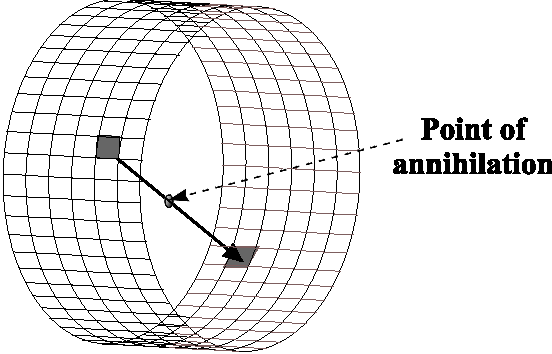
\includegraphics[scale=0.50]{ICCS/ringscanner}
  \caption{Two detectors register an event in a PET-scanner}
  \label{fig:scanner and detector}
\end{figure}

\subsubsection{The LM OSEM Algorithm}
List-Mode Ordered Subset Expectation Maximization \cite{ReaderErFlOt1998} (called LM OSEM in the sequel) is a block-iterative algorithm for 3D image reconstruction.
LM OSEM takes a set of events from a PET scanner and splits them into $s$ equally sized subsets.
Then, for each subset $S_l, l \in {0, \ldots, s-1}$, the following computation is performed:
\begin{equation}
  f_{l+1}=f_{l}c_{l};\quad c_{l}=\dfrac{1}{A_N^T \textbf{1}} \sum_{i \in S_{l}} (A_i)^T \dfrac{1}{A_{i} f_{l}}.
\label{equ:lm_osem}
\end{equation}

Here $f \in \mathbb{R}^n$ is a 3D image in vector form with dimensions $n = (X \times Y \times Z)$, $A$ it the so called system matrix, element $a_{ik}$ of row $A_i$ is the length of intersection of the line between the two detectors of event $i$ with voxel $k$ of the reconstruction image, computed with Siddon's algorithm \cite{Siddon1985}.
$\rfrac{1}{A_N^T \textbf{1}}$ is the so-called normalization vector; since it can be precomputed, we will omit it in the following.
The multiplication $f_{l}c_{l}$ is performed element-wise.
Each subset's computation takes its predecessor's output image as input and produces a new, more precise image.

The structure of a sequential LM OSEM implementation is shown in \autoref{lst:lmosem:seq_code}.
The outermost loop iterates over the subsets.
The first inner loop (step 1, lines~\autoref{lst:lmosem:seq_code:step1:begin}--\autoref{lst:lmosem:seq_code:step1:end}) iterates over subset's events to compute $c_l$, which requires three sub-steps:
row $A_i$ is computed from the current event using Siddon's algorithm;
the local error for row $A_i$ is computed and, finally, added to $c_l$.
The second inner loop (step 2, lines~\autoref{lst:lmosem:seq_code:step2:begin}--\autoref{lst:lmosem:seq_code:step2:end}) iterates over all elements of $f_l$ and $c_l$ to compute $f_{l+1}$.
\begin{figure}
\begin{lstlisting}[
  caption={Sequential code for LM OSEM comprises one outer loop with two nested inner loops.},
  label={lst:lmosem:seq_code}]
for (int l = 0; l < subsets; l++) {
  // read subset

  // step 1: compute error image $c_l$
  for (int i = 0; i < subset_size; i++) { $\label{lst:lmosem:seq_code:step1:begin}$
    // compute $A_i$
    // compute local error
    // add local error to $c_l$
  } $\label{lst:lmosem:seq_code:step1:end}$

  // step 2: update image estimate $f$
  for (int k = 0 ; k < image_size; k++) { $\label{lst:lmosem:seq_code:step2:begin}$
    if (c_l[k] > 0.0) { f[k] = f[k] * c_l[k]; }
  } $\label{lst:lmosem:seq_code:step2:end}$
}
\end{lstlisting}
\end{figure}

\subsubsection{Parallelization of LM OSEM in OpenCL}
\label{sec:parallel_implementation}
LM OSEM is a rather time-consuming algorithm that needs parallelization:
a typical 3D image reconstruction processing $6 \cdot 10^7$ input events for a $150 \times 150 \times 280$ voxel PET image takes more than two hours on a modern PC.

Although the iterations of the outer loop in \autoref{lst:lmosem:seq_code} are inherently sequential, we can parallelize the two calculation steps within one iteration as shown in \autoref{fig:lmosem:em_distribution} for a system comprising one CPU and two GPUs.
Note that these steps require different data distribution patterns:
\begin{itemize}
  \item[] \emph{Step 1:} Subset's events are copied from the CPU to all GPUs (\emph{upload}) to compute the summation part of $c_l$ concurrently. This step requires that the complete image estimate $f_l$ is available to all GPUs.
  \item[] \emph{Step 2:} For computing the next image estimate $f_{l+1}$ in parallel, the current image estimate $f_l$ and the error image $c_l$ computed in step 1 have to be distributed in disjoint parts (blocks) among all GPUs.
\end{itemize}

\begin{figure}
  \centering
  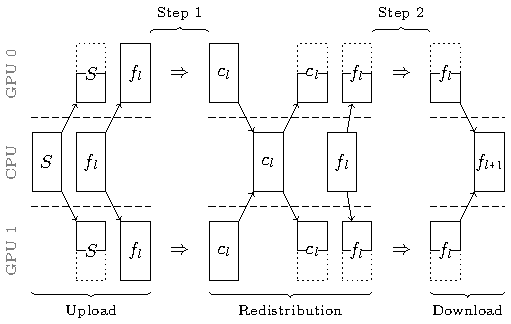
\includegraphics[width=0.6\textwidth]{ICCS/em_distribution}
  \caption{Parallelization schema of the LM OSEM algorithm.}
  \label{fig:lmosem:em_distribution}
\end{figure}
Thus, the parallelization schema in \autoref{fig:lmosem:em_distribution} requires a data \emph{redistribution} phase between the two computation steps.
During step 1, each GPU computes a partial sum of $c_l$ which are summed up and redistributed disjoinlty to all GPUs after step 1.
Note that for step 1, each GPU requires a full copy of the image estimate, while in step 2 all GPUs update disjoint parts of it.
After step 2, the disjoint parts of the image estimate are copied from all GPUs back to the CPU (\emph{download}).

\bigskip\noindent
In the following, we describe how the phases in the parallelization schema in \autoref{fig:lmosem:em_distribution} are implemented using OpenCL.

\paragraph{Upload}
\autoref{lst:lmosem:upload} shows the simplified OpenCL implementation of the upload phase.
Uploading of the event vector $S$ is performed in lines \autoref{lst:lmosem:upload:1:start}--\autoref{lst:lmosem:upload:1:end}, while lines \autoref{lst:lmosem:upload:2:start}--\autoref{lst:lmosem:upload:2:end} show the upload of the image estimate $f_l$.
In OpenCL, we have to manage each GPU explicitly, therefore, for each GPU, we create an array of buffers (\texttt{s\_gpu} in line~\autoref{lst:lmosem:upload:1:cl_false} and \texttt{f\_gpu} in line~\autoref{lst:lmosem:upload:2:cl_false}) and we use a loop (line \autoref{lst:lmosem:upload:loop}) to repeat all memory operations for each GPU.
For performance reasons, we use asynchronous copy operations, specified using the \texttt{CL\_FALSE} flag (lines \autoref{lst:lmosem:upload:1:cl_false} and \autoref{lst:lmosem:upload:2:cl_false}): this allows data transfers to multiple GPUs to overlap.
We perform different operations with $S$ (distribute among all GPUs) and $f_l$ (copy to each GPU), therefore, there are differences when specifying the amount of bytes to copy (lines \autoref{lst:lmosem:upload:1:amount} and \autoref{lst:lmosem:upload:2:amount}) and the offsets in the CPU memory (lines \autoref{lst:lmosem:upload:1:offset} and \autoref{lst:lmosem:upload:2:offset}).
Altogether eleven such memory operations -- each with different amounts of bytes and offsets -- appear in the OpenCL source code.

\begin{lstlisting}[float,
  caption={Implementation of the upload phase in OpenCL (omitting error checks for brevity)},
  label={lst:lmosem:upload}]
for (int gpu = 0; gpu < gpu_count; gpu++) {$\label{lst:lmosem:upload:loop}$
  // upload $S$
  clEnqueueWriteBuffer( command_queue[gpu], $\label{lst:lmosem:upload:1:start}$
        s_gpu[gpu], CL_FALSE, 0,$\label{lst:lmosem:upload:1:cl_false}$
        sizeof(float) * size_of_s / gpu_count,$\label{lst:lmosem:upload:1:amount}$
        (void*)&s_cpu[ gpu * size_of_s / gpu_count ],$\label{lst:lmosem:upload:1:offset}$
        0, NULL, NULL );$\label{lst:lmosem:upload:1:end}$

  // upload $f_l$
  clEnqueueWriteBuffer( command_queue[gpu], $\label{lst:lmosem:upload:2:start}$
        f_gpu[gpu], CL_FALSE, 0,$\label{lst:lmosem:upload:2:cl_false}$
        sizeof(float) * size_of_f,$\label{lst:lmosem:upload:2:amount}$
        (void*)&f_cpu[0],$\label{lst:lmosem:upload:2:offset}$
        0, NULL, NULL );$\label{lst:lmosem:upload:2:end}$
}
\end{lstlisting}

\paragraph{Step 1}
The implementation of step 1 performs the operations shown in \autoref{lst:lmosem:seq_code}.
Because of GPU memory restrictions, the OpenCL implementation is not straightforward, therefore, we will not show the detailed code here.
An OpenCL kernel is launched where each work item processes multiple events one after another.
For each event first $A_i$ is computed, then the local error for $A_i$ computed using the current image estimate $f_l$ which is finally added to $c_l$.

In the formula $A_i$ represents the \emph{path} of a detected line through the 3D image space.
In mathematics it is convenient to think as this as a sparse vector containing the length of the intersection of the line with a given voxel in the image space.
As most voxels are not intersected by the line, most entries in the vector remain zero.
Therefore, in the OpenCL code $A_i$ is represented as an array of pairs, where the first entry of each pair is the index of an voxel in the image space and the second entry is the length of the intersection with this voxel.

Synchronization between work items in OpenCL is highly restricted, \ie, synchronization is only possible for work items organized in the same work group.
Therefore, it is not possible to efficiently protect the writing operation to $c_l$ to avoid race conditions.
We have conducted studies and found that for this particular algorithm these race conditions are acceptable as they do not substantially decrease the numerical accuracy of the computed result~\cite{SchellmannGoMeKoScWuBu2009}.


\paragraph{Redistribution}

\begin{lstlisting}[float,
  caption={OpenCL pseudocode for the redistribution phase},
  label={lst:lmosem:redistribution}]
// download all c_l values from the GPUs to the CPU
cl_event events[gpu_count];
for (int gpu = 0; gpu < gpu_count; gpu++) {
  clEnqueueReadBuffer( ..., &events[gpu] );$\label{lst:lmosem:redistribution:operation}$
}
clWaitForEvents(gpu_count, events);$\label{lst:lmosem:redistribution:wait}$

// combine data on CPU
combine( ... );$\label{lst:lmosem:redistribution:combine}$

// upload block of the new c_l version to each GPU
for (int gpu = 0; gpu < gpu_count; gpu++) {
  clEnqueueWriteBuffer( ... );
}
\end{lstlisting}

\autoref{lst:lmosem:redistribution} shows an OpenCL pseudocode for the redistribution phase.
To download the data from all GPUs, we use the \texttt{clEnqueueReadBuffer} function and perform the operations asynchronously, but this time, we have to wait for the operations to finish.
For such synchronization, OpenCL uses \emph{events}, associated with an operation (line \autoref{lst:lmosem:redistribution:operation}) for waiting for the operation to finish (line \autoref{lst:lmosem:redistribution:wait}).
After all downloads have finished, we combine the different values of $c_l$ to a new value of $c_l$ on the CPU (line \autoref{lst:lmosem:redistribution:combine}), and upload the blocks of $c_l$ to the GPUs.
Even if we only copied data between GPUs, without processing them on the CPU, we still would have to download them to the CPU because direct GPU-to-GPU transfers are currently not possible in OpenCL.

\paragraph{Step 2}
\autoref{lst:lmosem:step_2} shows the implementation of step 2.
In OpenCL, computations are specified as \emph{kernels} which are created from the source code specifying the computation.
The computation in step 2 is, therefore, described as a string in lines \autoref{lst:lmosem:step_2:string:start}--\autoref{lst:lmosem:step_2:string:stop}.
The operations used here are the same as in the sequential code.

For executing the computations of step 2, we have to perform the following steps for each GPU:
\begin{itemize}
  \item create an OpenCL kernel from the source code (requires 50 lines of code in OpenCL);
  \item compile the kernel specifically for the GPU (requires 13 lines of code in OpenCL);
  \item specify kernel arguments one-by-one using the \texttt{clSetKernelArg} function (line \autoref{lst:lmosem:step_2:args:start} -- \autoref{lst:lmosem:step_2:args:stop});
  \item specify execution environment, i.\,e., how many instances of the kernel to start (line \autoref{lst:lmosem:step_2:env:start} -- \autoref{lst:lmosem:step_2:env:stop});
  \item launch the kernel (line \autoref{lst:lmosem:step_2:kernel:start} -- \autoref{lst:lmosem:step_2:kernel:stop}).
\end{itemize}
\begin{lstlisting}[float,
  caption={Implementation of step 2 in OpenCL (omitting error checks for brevity)},
  label={lst:lmosem:step_2}]
// step 2 (in $\autoref{fig:lmosem:em_distribution}$)
source_code_step_2 =
  "kernel void step2(global float* f, global float* c_l,$\label{lst:lmosem:step_2:string:start}$
                     int offset, int size) {
    int id = get_global_id(0) + offset;
    if (id < size && c_l[id] > 0.0){ f[id] = f[id]*c_l[id];}$\label{lst:lmosem:step_2:zip}$
   }";$\label{lst:lmosem:step_2:string:stop}$

for (int gpu = 0; gpu < gpu_count; gpu++) {
  // create kernel (50 lines of code)
  // compile kernel (13 lines of code)

  // specifying kernel arguments:
  clSetKernelArg(kernel_step2[gpu], 0, sizeof(cl_mem),$\label{lst:lmosem:step_2:args:start}$
                 (void*)&f_buffer[gpu]);
  clSetKernelArg(kernel_step2[gpu], 1, sizeof(cl_mem),
                 (void*)&c_l_buffer[gpu]);
  int offset = gpu * (size_of_f / gpu_count);
  clSetKernelArg(kernel_step2[gpu], 2, sizeof(int),
                 (void*)&offset);
  int size   = MIN( (gpu + 1) * (size_of_f / gpu_count),
                    size_of_f );
  clSetKernelArg(kernel_step2[gpu], 3, sizeof(int),
                 (void*)&size);$\label{lst:lmosem:step_2:args:stop}$

  // specify execution environment
  int local_work_size[1]  = { 32 };$\label{lst:lmosem:step_2:env:start}$
  int global_work_size[1] =
        { roundUp(32, size_of_f / gpu_count) };$\label{lst:lmosem:step_2:env:stop}$
  // launch the kernel
  clEnqueueNDRangeKernel($\label{lst:lmosem:step_2:kernel:start}$
        command_queue[gpu], kernel_step2[gpu],
        1, NULL, &global_work_size, &local_work_size, 0,
        NULL, NULL); }$\label{lst:lmosem:step_2:kernel:stop}$
\end{lstlisting}


\paragraph{Download}
The implementation of the download phase is similar to the upload phase as shown in \autoref{lst:lmosem:upload}.


% ============================================================================ %
\subsection{Requirements to a High-Level Programming Model}
\label{section:requirements}
The described implementation of the example application reveals the main problems and challenges that application developers have to overcome when targeting \GPU systems.
Our analysis show that to simplify programming for a system with multiple \GPUs, at least the following three high-level abstraction are desirable:

\paragraph{Parallel container data types}
Compute intensive applications typically operate on a (possibly big) set of data items.
As shown in \autoref{lst:lmosem:upload}, managing memory is error-prone because low-level details, like offset calculations, have to be programmed manually.

A high-level programming model should be able to make collections of data automatically accessible to all processors in a system and it should provide an easy-to-use interface for the application developer.

\paragraph{Recurring patterns of parallelism}
While each application (of course) performs different concrete operations, the general structure of parallelization resembles parallel patterns that are commonly used in many applications.
In step~1, for computing the error image~$c_l$, the same sequence of operations is performed for every event from the input subset, which is the well-known \emph{map} pattern of data-parallel programming~\cite{GorlatchCo2011}.
In step~2, two images (the current image estimate~$f_l$ and the error image~$c_l$) are combined element-wise into the output image~($f_{l+1}$), see line~\autoref{lst:lmosem:step_2:zip} of \autoref{lst:lmosem:step_2}, which is again a well-known pattern of parallelism commonly called \emph{zip}.

It would be, therefore, desirable to express the high-level structure of an application using pre-defined common patterns, rather than describing the parallelism manually in much detail.

\paragraph{Distribution and redistribution mechanisms}
To achieve scalability of applications on systems comprising multiple \GPUs, it is crucial to decide how the application's data are distributed across all available \GPUs.
Distributing and re-distributing data in \OpenCL is cumbersome because data transfers have to be managed manually and performed via the \CPU, as shown in \autoref{lst:lmosem:upload} and \autoref{lst:lmosem:redistribution}.

Therefore, it is important for a high-level programming model to allow both for describing the data distribution and for changing the distribution at runtime.


% ============================================================================ %
% ============================================================================ %
\section{The SkelCL Programming Model}
\label{section:skelcl-programming-model}
\SkelCL (Skeleton Computing Language) is a high-level programming model targeting multi-\GPU system.
It is developed as an extension of the standard \OpenCL programming model~\cite{OpenCL}.

\SkelCL adds three main high-level features to \OpenCL which we identified as desirable in~\autoref{section:requirements}:

\begin{itemize}
  \item \emph{parallel container data types} for unified memory management between \CPU and (multiple) \GPUs;
  \item \emph{recurring patterns of parallelism} (\aka \emph{algorithmic skeletons}) for easily expressing parallel computation patterns;
  \item \emph{data distribution} and \emph{redistribution} mechanisms for transparent data transfers in multi-\GPU systems.
\end{itemize}

\noindent
\SkelCL inherits all advantageous properties of \OpenCL, including its portability across different heterogeneous parallel systems.
\SkelCL is designed to be fully compatible with \OpenCL: arbitrary parts of a \SkelCL code can be written or rewritten in \OpenCL, without influencing program's correctness.

In the remainder of this section we discuss the design of the \SkelCL programming model in more detail.
Its implementation as a \Cpp library will be discussed in the next section.

% ============================================================================ %
\subsection{Parallel Container Data Types}
\label{section:skelcl-programming-model:container}
\SkelCL offers the application developer two container classes -- vector and matrix -- which are transparently accessible by both, \CPU and \GPUs (or using \OpenCL's terminology, host and devices).
The \emph{vector} abstracts a one-dimensional contiguous memory area while the \emph{matrix} provides an interface to a two-dimensional memory area.
The \SkelCL container data types have two major advantages as compared with \OpenCL.

The first advantage is its automatic memory management.
When a container is created on the host, memory is allocated on the devices automatically;
when a container on the host is deleted, the memory allocated on the devices is freed automatically.
In \OpenCL memory has to be allocated and freed manually.

The second advantage is that the necessary data transfers between the host and devices are performed automatically and implicitly.
Before performing a computation on container types, the \SkelCL system ensures that all input containers' data is available on all participating devices.
This may result in implicit data transfers from the host to device memory, which in \OpenCL requires explicit programming, as we saw in~\autoref{lst:lmosem:upload} in~\autoref{section:opencl-example}.
Similarly, before any data is accessed on the host, the implementation of \SkelCL implicitly ensures that this data on the host is up-to-date by performing necessary data transfers automatically.
Using the \code{clEnqueueWriteBuffer} (see lines~\ref{lst:lmosem:upload:1:start}--\ref{lst:lmosem:upload:1:end} in \autoref{lst:lmosem:upload}) and \code{clEnqueueReadBuffer} (see \autoref{lst:lmosem:redistribution}) functions nine arguments have to be specified to perform a single data transfer in \OpenCL.
The \SkelCL container classes shield the programmer from these low-level operations like memory allocation (on the devices) and data transfers between host and device.

Developing applications on two-dimensional data for modern parallel architectures is cumbersome and challenging, since efficient memory handling is essential for achieving good performance.
In case of \GPUs, exploiting the memory hierarchy by using the fast but small on-chip memory is key for high performance.
Therefore, in addition to the vector as a one-dimensional abstract data structure, \SkelCL offers a specific abstract data type for handling two-dimensional data, the matrix.
We will see later in \autoref{sec:opt_allpairs_skeleton} and \autoref{section:skelcl-library} how \SkelCL automatically exploits the memory hierarchy to improve performance.

% The implementations of the algorithmic skeletons included in \SkelCL differentiate for their input container between vector and matrix, thus, offering optimized implementations for each case.


\subsection{Algorithmic Skeletons}
\label{section:skelcl-programming-model:skeletons}
In original \OpenCL, computations are expressed as compute \emph{kernels} which are executed in a parallel manner on an \OpenCL device, \eg, a \GPU.
As seen earlier in \autoref{section:opencl-example} the application developer must explicitly specify the parallelism by indicating how many instances of a kernel (called \emph{work items}) should be launched in parallel.
In \autoref{lst:lmosem:step_2} the \code{local\_work\_size} (line~\ref{lst:lmosem:step_2:env:start}) and \code{global\_work\_size} (line~\ref{lst:lmosem:step_2:env:global}) specify the number of work items and how they are organized into groups.
The programmer must ensure that these numbers match,\ie, that the global size is evenly divisible by the local size.
Communications between work items are limited and have to be implemented carefully to avoid race conditions and deadlocks.
In addition, kernels take pointers to device memory as input and contain program code for reading/writing single data items from/to it.
These pointers are unsafe as they have to be used carefully, because no boundary checks are performed by \OpenCL.

To shield the application developer from these low-level programming issues, \SkelCL extends \OpenCL by introducing high-level programming patterns, called \emph{algorithmic skeletons}~\cite{Cole1991}.
Formally, a skeleton is a higher-order function that executes one or more user-defined (so-called \emph{customizing}) functions in a pre-defined parallel manner, thus hiding the details of parallelism and communication from the user~\cite{GorlatchCo2011}.

\SkelCL provides four basic data-parallel skeletons: \map, \zip, \reduce, and \scan,
as well as two more advanced skeletons targeting specific application domains: \stencil and \allpairs.
In this section we will look at the basic skeletons, the advanced skeletons will be discussed in~\autoref{section:skelcl-programming-model:specialSkeletons}.
The four basic skeletons have been selected, because they have been proven to be useful for a broad range of applications.
Moreover, these skeletons can be efficiently implemented on \GPUs as their computation patterns match the data-parallel \SIMD (Singe Instruction, Multiple Data) execution model implemented by \GPUs.


\paragraph{The \map skeleton}
The \map skeleton is a well-known basic algorithmic skeleton, applying the customizing function to each element of a container in parallel.
This skeleton originates from the functional world, where the \code{map} function is recognized as an important primitive for writing high-level code.
In many programming languages an equivalent sequential function exists, either known under the same name, like in Haskell or Python, or by other names, like \code{transform} in \Cpp.

In \SkelCL the \map skeleton can operate on vectors as well as matrices.
We start by formally defining the skeleton on vectors:
\begin{definition}
  \label{definition:map}
  Let $\vec{x}$ be a vector of size $n$ with elements $x_i$ where $0 < i \leq n$.
  Let $f$ be a unary customizing function defined on elements.
  The algorithmic skeleton \map is then defined as follows:
  \begin{equation*}
    \map\ f\ [x_1, x_2, \dots, x_n] \eqdef [f\ x_1, f\ x_2, \dots, f\ x_n]
  \end{equation*}
\end{definition}
\noindent
The definition for matrices is similar:
\begin{definition}
  \label{definition:map:matrix}
  Let $M$ be an $n\times m$ matrix with elements $m_{i,j}$ where $0 < i \leq n$ and $0 < j \leq m$.
  Let $f$ be a unary customizing function.
  The algorithmic skeleton \map is defined as follows:
  \begin{equation*}
    \map\ f\ \DottedMatrix{m_{0,0}}{m_{0,m}}{m_{n,0}}{m_{n,m}}
      \eqdef \DottedMatrix{f\ m_{0,0}}{f\ m_{0,m}}{f\ m_{n,0}}{f\ m_{n,m}}
  \end{equation*}
\end{definition}
\noindent
The output container of the \map skeleton, either vector or matrix, can be computed in parallel, because the computation of each single element is independent of each other.

A simple possible application of the \map skeleton is negating all the values in a vector:
\begin{align*}
  neg\ \vec{x} &= \map\ (-)\ \vec{x}
\end{align*}


\paragraph{The \zip skeleton}
The \zip skeleton operates on two containers and combines them into one.
As the \map skeleton it is defined for vectors and matrices as well.
\begin{definition}
  \label{definition:zip}
  Let $\vec{x}$ and $\vec{y}$ be vectors of size $n$ with elements $x_i$ and $y_i$ where $0 < i \leq n$.
  Let $\oplus$ be a binary customizing operator.
  The algorithmic skeleton \zip is defined as follows:
  \begin{equation*}
    \begin{split}
      \zip\ \oplus\ [x_1, x_2, \dots, x_n]\ [y_1, y_2, \dots, y_n]\\
      \eqdef [x_1 \oplus y_1, x_2 \oplus y_2, \dots, x_n \oplus y_n]
    \end{split}
  \end{equation*}
\end{definition}
\noindent
Again the definition for matrices is similar:
\begin{definition}
  \label{definition:zip:matrix}
  Let $M$ and $N$ be $n\times m$ matrices with elements $m_{i,j}$ and $n_{i,j}$ where $0 < i \leq n$ and $0 < j \leq m$.
  Let $\oplus$ be a binary customizing operator.
  The algorithmic skeleton \zip is defined as follows:
  \begin{equation*}
    \begin{split}
      \zip\ f\ {\DottedMatrix{m_{0,0}}{m_{0,m}}{m_{n,0}}{m_{n,m}}}\
            {\DottedMatrix{n_{0,0}}{n_{0,m}}{n_{n,0}}{n_{n,m}}} \\
      \eqdef \DottedMatrix{m_{0,0} \oplus n_{0,0}}{m_{0,m} \oplus n_{0,m}}{m_{n,0} \oplus n_{n,0}}{m_{n,m} \oplus n_{n,m}}
    \end{split}
  \end{equation*}
\end{definition}
\noindent
This definitions require the two input containers to be of exactly the same size.
The \zip skeleton is parallelizeable in the same manner as \map, as each element of the output container can be computed in parallel.

A possible application of the \zip skeleton is performing pairwise addition of two vectors:
\begin{align*}
  add\ \vec{x}\ \vec{y} = \zip\ (+)\ \vec{x}\ \vec{y}
\end{align*}


\paragraph{The \reduce skeleton}
The \reduce skeleton computes a single value from a vector by successively applying the binary customizing function.
In \SkelCL the \reduce skeleton is only defined on vectors:
\begin{definition}
  \label{definition:reduce}
  Let $\vec{x}$ be a vector of size $n$ with elements $x_i$ where $0 < i \leq n$.
  Let $\oplus$ be an associative binary customizing operator with the corresponding identity element \id.
  The algorithmic skeleton \reduce is defined as follows:
  \begin{equation*}
    \reduce\ \oplus\ \id\ [x_1, x_2, \dots, x_n]
      \eqdef x_1 \oplus x_2 \oplus \dots \oplus x_n
  \end{equation*}
\end{definition}
\noindent
Requiring the operator to be associative enables efficient parallel implementations.
The identity element \id can be used by the implementation, \eg, to initialize intermediate buffers.

A possible application of the \reduce skeleton is to finding the maximum value of a vector:
\begin{align*}
  maxValue\ \vec{x} &= \reduce\ max\ 0\ \vec{x}\\
  \text{where:} \qquad max\ a\ b &=
    \left\{
      \begin{array}{l l}
      a & \text{if } a \geq b\\
      b & \text{if } a < b
      \end{array}
    \right.
\end{align*}


\paragraph{The \scan skeleton}
The \scan skeleton (\aka prefix-sum) yields an output vector with each element obtained by applying the customizing function to the elements of the input vector up to the current element's index.
In \SkelCL, the \scan skeleton is only defined on vectors:
\begin{definition}
  \label{definition:scan}
  Let $\vec{x}$ be a vector of size $n$ with elements $x_i$ where $0 < i \leq n$.
  Let $\oplus$ be an associative binary customizing operator with the corresponding identity element \id.
  The algorithmic skeleton \scan is defined as follows:
  \begin{equation*}
    \begin{split}
      \scan&\ \oplus\ \id\ [x_1, x_2, \dots, x_n] \\
      &\eqdef [\id, x_1 \oplus x_2,\ \dots,x_1 \oplus x_2 \oplus \cdots \oplus x_n]
    \end{split}
  \end{equation*}
\end{definition}
\noindent
Even though the \scan pattern seems inherently sequential, because each individual result contains the results of its predecessor, efficient parallel implementations do exist for this problem.
Blelloch~\cite{Blelloch1991} studies this parallel pattern in great detail and efficient implementations for \GPUs exist~\cite{HarrisSeOw2007} following his algorithmic ideas.

A possible application of the \scan skeleton is the computation of the prefix sum which can be used as part of the counting sort algorithm~\cite{Knuth1998} or for solving the list ranking problem~\cite{ColeVi1989}.
\begin{align*}
  prefixSum\ \vec{x} = \scan\ (+)\ 0\ \vec{x}
\end{align*}

\paragraph{Parallel Programming with Algorithmic Skeletons}
In \SkelCL, rather than writing low-level kernels, the application developer customizes suitable skeletons by providing application-specific functions which are often much simpler than kernels as they specify an operation on basic data items rather than containers.

Skeletons can be customized and composed to express complex algorithms.
To demonstrate how to express computations with algorithmic skeletons let us consider three simple linear algebra applications:
scaling a vector with a constant, computing the sum of absolute values of a vector, and computing the dot product (\aka inner product) of two vectors.
These three applications are all part of the well-known \emph{Basic Linear Algebra Subprograms (\BLAS)}~\cite{Dongarra2002,Dongarra2002a} library.

For scaling a vector with a constant $\alpha$ we use the \map skeleton:
\begin{align*}
  scal\ \vec{x}&= \map\ f_{\alpha}\ \vec{x}\\
  \text{where:} \qquad f_{\alpha}\ x_i &= \alpha \cdot x_i
\end{align*}

\noindent
For computing the sum of absolute values we compose a \map and \reduce skeleton.
%We use the $\circ$ to denote the sequential composition of two functions, \ie\ $(f \circ g)\ x = f(g\ x)$.
\begin{align*}
  %asum\ \vec{x} &= \big(\ \reduce\ (+)\ 0\ \circ \map\ abs\ \big)\ \vec{x}\\
  asum\ \vec{x} &= \reduce\ (+)\ 0\ \big(\ \map\ abs\ \vec{x}\ \big)\\
  %asum &= \reduce\ (+)\ 0\ \circ \map\ abs\\
  \text{where:} \qquad abs\ a &=
    \left\{
      \begin{array}{r l}
      a & \text{if } a \geq 0\\
      -a & \text{if } a < 0
      \end{array}
    \right.
\end{align*}

\noindent
To compute the dot product of two vectors we compose a \zip skeleton customized with multiplication and a \reduce skeleton customized with addition:
\begin{align*}
  %dot\ \vec{x}\ \vec{y} &= \big(\ \reduce\ (+)\ 0\ \circ \zip\ (\times)\ \vec{x}\ \big)\ \vec{y}\\
  dot\ \vec{x}\ \vec{y} &= \reduce\ (+)\ 0\ \big(\ \zip\ (\times)\ \vec{x}\ \vec{y}\ \big)
\end{align*}

\noindent
Algorithmic skeletons are not limited to linear algebra applications, but can be used to implement a boarded range of application types as we will discuss in \autoref{chapter:skelcl-evaluation}.
Among others, we will see an algorithmic skeleton based implementation of the real-world medial imaging application example discussed at the beginning of this chapter.


% ============================================================================ %
\subsection{Data distribution and redistribution}
\label{section:skelcl-programming-model:distribution}

For multi-device systems, \SkelCL's parallel container data types (vector and matrix) abstract from the separate memory areas on multiple \OpenCL devices, \ie, container's data is accessible by each device.
Each device may access different parts of a container or may even not access it at all.
For example, when implementing work-sharing on multiple \GPUs, the \GPUs will access disjoint parts of input data, such that copying only a part of the vector to a \GPU would be more efficient than copying the whole data to each \GPU.

To simplify the partitioning of a container on multiple devices, \SkelCL introduces the concept of \emph{distributions}.
A distribution describes how the container's data is distributed among the available devices.
It allows the application developer to abstract from the challenges of managing memory ranges which are shared or partitioned across multiple devices: the programmer can think of a distributed container as of a self-contained entity.



\begin{figure}[tb]
  \centering
  \begin{subfigure}{.3\textwidth}
    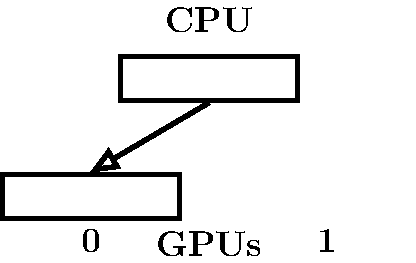
\includegraphics[width=\textwidth]{PaCT/singleDistribution_vector}
    \caption{\emph{single}}
    \label{fig:distributions:single}
  \end{subfigure}
  \hfill
  \begin{subfigure}{.3\textwidth}
    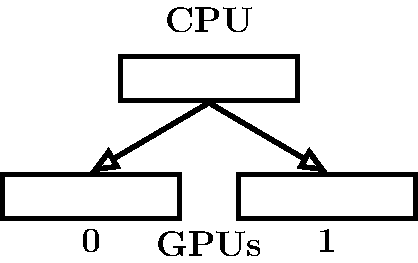
\includegraphics[width=\textwidth]{PaCT/copyDistribution_vector}
    \caption{\emph{copy}}
    \label{fig:distributions:copy}
  \end{subfigure}
  \hfill
  \begin{subfigure}{.3\textwidth}
    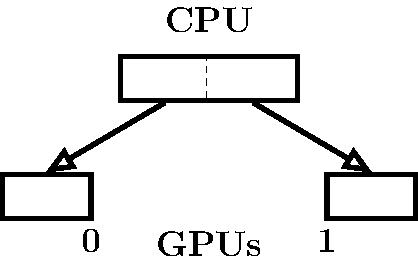
\includegraphics[width=\textwidth]{PaCT/blockDistribution_vector}
    \caption{\emph{block}}
    \label{fig:distributions:block}
  \end{subfigure}
  \caption{Distributions of a vector in SkelCL.}
  \label{fig:distributions}
  \bigskip
\end{figure}

\begin{figure}[tbp]
  \centering
  \begin{subfigure}{.22\textwidth}
    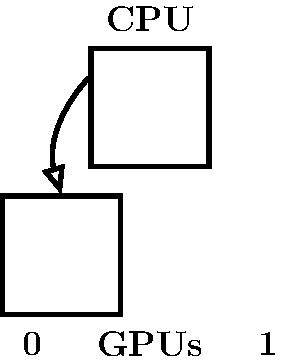
\includegraphics[width=\textwidth]{PaCT/singleDistribution_matrix}
    \caption{\emph{single}}
    \label{fig:distributions_matrix:single}
  \end{subfigure}
  \hfill
  \begin{subfigure}{.22\textwidth}
    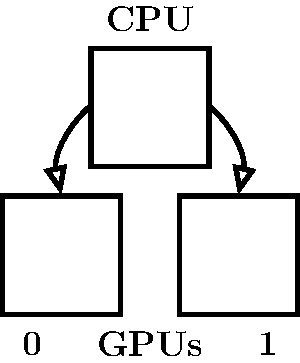
\includegraphics[width=\textwidth]{PaCT/copyDistribution_matrix}
    \caption{\emph{copy}}
    \label{fig:distributions_matrix:copy}
  \end{subfigure}
  \hfill
  \begin{subfigure}{.22\textwidth}
    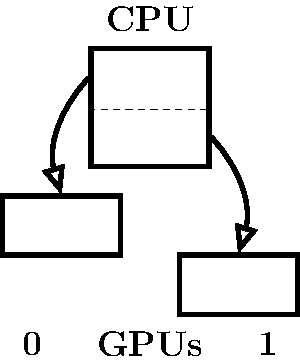
\includegraphics[width=\textwidth]{PaCT/blockDistribution_matrix}
    \caption{\emph{block}}
    \label{fig:distributions_matrix:block}
  \end{subfigure}
  \caption{Distributions of a matrix in SkelCL.}
  \label{fig:distributions_matrix}
\end{figure}


Three kinds of basic distributions are currently available in \SkelCL:
\emph{single}, \emph{copy}, and \emph{block} (see \autoref{fig:distributions} for distributing a vector on a system with two \GPUs).
If distribution is set to \emph{single} (\autoref{fig:distributions:single}), then vector's whole data is stored on a single \GPU (the first \GPU if not specified otherwise).
The \emph{copy} distribution (\autoref{fig:distributions:copy}) copies vector's entire data to each available \GPU.
With the \emph{block} distribution (\autoref{fig:distributions:block}), each \GPU stores a contiguous, disjoint chunk of the vector.

The same three distributions are provided also for the matrix data type as shown in \autoref{fig:distributions_matrix}.
The \emph{block} distribution (\autoref{fig:distributions_matrix:block}) splits the matrix into chunks of rows, which simplifies the implementation.

% In particular the overlap distribution splits the matrix into one chunk for each GPU; in addition, each chunk contains a number of continuous rows from the neighboring chunks.
% A parameter -- the \emph{overlap size} -- specifies the number of rows at the borders of a chunk which are copied to the two neighboring GPUs.
% \autoref{fig:Distribution_matrix:overlap} illustrates the overlap distribution:
% GPU 0 receives the top chunk ranging from the top row to the middle, while GPU 1 receives the second chunk ranging from the middle row to the bottom.
% The marked parts are called \emph{overlap region} they are the same on both GPUs.

The application developer can set the distribution of containers explicitly, otherwise every skeleton selects a default distribution for its input and output containers.
Container's distribution can be changed at runtime:
this implies data exchanges between multiple \GPUs and the \CPU, which are performed by the \SkelCL implementation implicitly.
As seen earlier in this chapter (\autoref{lst:lmosem:redistribution}) implementing such data transfers in the standard \OpenCL is a cumbersome task:
data has to be downloaded to the \CPU before it is uploaded to the \GPUs, including the corresponding length and offset calculations;
this results in a lot of low-level code which becomes completely hidden when using \SkelCL.

A special situation arises when the distribution is changed from the \emph{copy} distribution to any other distribution.
In this case each \GPU holds its own full copy of the data which might have been modified locally on each \GPU.
In order to maintain \SkelCL's concept of a self-contained container, these different versions are combined using a user-specified function when the distribution is changed.
If no function is specified, the copy of the first \GPU is taken as the new version of the container; the copies of the other \GPUs are discarded.


% ============================================================================ %
\subsection{More Complex Algorithmic Skeletons}
\label{section:skelcl-programming-model:specialSkeletons}

The basic algorithmic skeletons presented in~\autoref{section:skelcl-programming-model:skeletons} are long known in the functional and algorithmic skeleton communities.
In this section we will introduce two new more advanced algorithmic skeletons, which are more restrictive.
By limiting the use cases of these novel algorithmic skeleton we are able to make more assumptions in the implementation and provide advanced optimizations on modern multi-\GPU systems.

The first new skeleton (\stencil) is targeted towards \emph{stencil} (\aka nearest neighbor) computations, which are computations performed for every element of a container while including neighboring elements in the computation.
The second new skeleton (\allpairs) combines two matrix containers in an all-to-all fashion, which is a pattern used in applications like n-body simulation or matrix matrix multiplication.

For both skeletons we will first formally define them before looking at possible use cases.
Their implementations targeting multi-\GPU systems will be described in~\autoref{section:skelcl-library}.


\subsubsection{The \stencil Skeleton}

Many numerical and image processing applications dealing with two-dimensional data perform calculations for a particular data element taking neighboring data elements into account.
These type of applications are also known as \emph{stencil} or \emph{nearest neighbor} applications.
To facilitate the development of such applications, we introduce the \stencil skeleton that can be used with both vector and matrix data type.

The \stencil skeleton is customized with three parameters: a unary function $f$, an integer value $d$, and an out-of-bounds function $h$.
The skeleton applies $f$ to each element of an input container while taking the neighboring elements within the range $d$ in each dimension into account.
When neighboring elements are accesses at the boundaries of the container out of bound accesses occur.
In these cases the function $h$ is called with the index causing the out of bound access and should return a replacement value.
We now formally define the \stencil skeleton. We start with the definition for vectors:
\begin{definition}
  \label{definition:mapoverlap}
  Let $\vec{x}$ be a vector of size $n$ with elements $x_i$ where $0 < i \leq n$.
  Let $f$ be a customizing function, $d$ be a positive integer value, and $h$ be an out-of-bound handling function.
  The algorithmic skeleton \stencil is defined as follows:
  \begin{equation*}
    \begin{split}
    &\stencil\ f\  d\ h\ [x_1, x_2, \ldots, x_n] \eqdef [y_1, y_2, \dots, y_n]\\
    &\text{where}\\[.5em]
    &\qquad y_i = f\ [x_{i-d}, \ldots, x_{i+d}] \qquad \forall\ i :  0 < i \leq n\\
    &\text{and\hfill}\\
    &\qquad x_j = h\ j \qquad \forall\ j : -d < j \leq 0\ \vee n < j \leq n+d
    \end{split}
  \end{equation*}
\end{definition}

\noindent
The definition for matrices is similar:
\begin{definition}
  \label{definition:mapoverlap:matrix}
  Let $M$ be an $n\times m$ matrix with elements $m_{i,j}$ where $0 < i \leq n$ and $0 < j \leq m$.
  Let $f$ be a customizing function, $d$ be an positive integer value, and $h$ be a out of bound handling function.
  The algorithmic skeleton \stencil is defined as follows:
  \begin{equation*}
    \begin{split}
    & \stencil\ f\  d\ h\ \DottedMatrix{m_{0,0}}{m_{0,m}}{m_{n,0}}{m_{n,m}}
               \eqdef \DottedMatrix{n_{0,0}}{n_{0,m}}{n_{n,0}}{n_{n,m}}\\
               &\text{where}\\[.5em]
    &\qquad n_{i,j} = f\ \DottedMatrix{m_{i-d,j-d}}{m_{i-d,j+d}}{m_{i+d,j-d}}{m_{i+d,j+d}} \qquad \forall\ i,j
        \begin{array}{r} 0 < i \leq n,\\ 0 < j \leq m \end{array}\\
        &\text{and}\\
    &\qquad m_{i,j} = h\ i\ j \qquad \forall\ i,j \begin{array}{r} -d < j \leq 0\ \vee n < j \leq n+d,\\ -d < j \leq 0\ \vee m < j \leq m+d \end{array}
    \end{split}
  \end{equation*}
\end{definition}


SkelCL currently supports a fixed set of choices for the out-of-bound handling function $h$ motivated by common cases of of bound handling in image processing applications.
This restriction could easily be lifted in the future.
The \stencil skeleton can currently be configured to handle out of bound accesses in two possible ways:
\begin{enumerate}
  \item a specified neutral value is returned (\ie, the out of bound function $h$ is constant);
  \item the nearest valid value inside the container is returned.
\end{enumerate}

Possible applications for the \stencil skeleton are image processing applications or physics simulations (see~\autoref{sec:imageProcessing} and \autoref{sec:physicsSim}).
A simple example application is the \emph{discrete Laplacian operator} used in image processing, \eg, for edge detection~\cite{Umbaugh1997}.
It computes a new value for every pixel of an image by weighting and summing up its direct neighboring pixel values, as follows:
\begin{align*}
  laplacian&\ M = \stencil\ f\ 1\ \overline{0}\ M\\
  \text{where:} \ \ &
  \begin{array}{ll}%
  f&\ \left[\begin{array}{ccc}%
      \hspace{-.5em} m_{i-1,j-1}& \hspace{-.5em} m_{i-1,j} & \hspace{-.5em}m_{i-1,j+1}\vspace{-.25em}\\%
      \hspace{-.5em} m_{i,j-1}  & \hspace{-.5em} m_{i,j}   & \hspace{-.5em}m_{i,j+1}  \vspace{-.25em}\\%
      \hspace{-.5em} m_{i+1,j-1}& \hspace{-.5em} m_{i+1,j} & \hspace{-.5em}m_{i+1,j+1}
    \end{array}\right] = \\[2em]
          &\ m_{i-1,j} + m_{i,j-1} - 4 \times m_{i,j} + m_{i,j+1} + m_{i+1,j}
  \end{array} \\
  \text{and } \overline{0} \text{ is th}&\text{e constant function always returning 0.}
\end{align*}

\subsubsection{The overlap data distribution}

\begin{figure}[tb]
  \centering
  \begin{subfigure}[b]{.3\textwidth}
    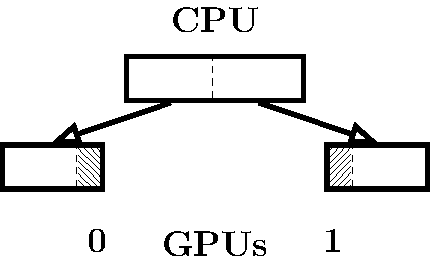
\includegraphics[width=\textwidth]{PaCT/overlapDistribution_vector}
    \caption{\emph{overlap}}
    \label{fig:overlap_distribution}
  \end{subfigure}
  \hspace{3em}
  \begin{subfigure}[b]{.22\textwidth}
    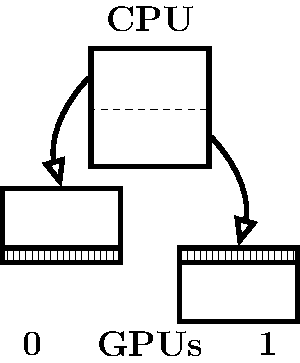
\includegraphics[width=\textwidth]{PaCT/overlapDistribution_matrix}
    \caption{\emph{overlap}}
    \label{fig:overlap_distribution:matrix}
  \end{subfigure}
  \caption{Overlap distribution of a vector and matrix in SkelCL.}
  \label{fig:overlap_distribution}
  \bigskip
\end{figure}

Together with the \stencil skeleton we introduce a new distribution called \emph{overlap} (Figure~\ref{fig:overlap_distribution}).
The overlap distribution splits the container into one chunk for each device, similarly to the \emph{block} distribution.
In addition, each chunk consists of a number of continuous elements (in case of the vector) or rows (in case of the matrix) which are copied to the neighboring devices, similar to the \emph{copy} distribution.
Therefore, the overlap distribution can be seen as a combination of the \emph{block} and \emph{copy} distribution.
The number of elements or rows at the edges of a chunk which are copied to the neighboring devices are called the \emph{overlap size}.

The \emph{overlap} distribution ensures that neighboring elements are always accessible even if the container is split across multiple devices.
The \emph{overlap} distribution is, therefore, automatically selected as distribution by the \stencil skeleton automatically setting the overlap size to the skeleton parameter $d$, which ensures that every device has access to the necessary neighboring elements.





\subsubsection{The \allpairs Skeleton}
\label{sec:allpairs_skeleton}

\emph{Allpairs computations} occur in a variety of applications, ranging from matrix multiplication and N-Body simulations in physics~\cite{AroraShVu2009} to pairwise Manhattan distance computations in bioinformatics~\cite{ChangDeQuRo2009}.
These applications share a common computational pattern:
for two sets of entities, the same computation is performed independently for all pairs in which entities from the first set are combined with entities from the second set.
We define the \allpairs skeleton to simplify the development of such applications.
We represent the entries of both sets as vectors of length $d$, where the cardinality of the first set is $n$ and the cardinality of the second set is $m$.
We model the first set as a $n\times d$ matrix $A$ and the second set as a $m\times d$ matrix $B$.
The allpairs computation yields an output matrix $C$ of size $n\times m$ with $c_{i, j} = a_i \oplus b_j$, where $a_i$ and $b_j$ are row vectors of $A$ and $B$, correspondingly,
%:
%$a_i = [a_{i,1}, \cdots, a_{i, d}]$, $b_j = [b_{j,1}, \cdots, b_{j,d}]$,
and $\oplus$ is a binary operator defined on vectors.

We formally define the \allpairs skeleton as follows:

\begin{definition}
  \label{def:allpairs}
  Let $A$ be a $n\times d$ matrix, $B$ be a $m\times d$ matrix, and $C$ be a $n\times m$ matrix, with their elements $a_{i,j}$, $b_{i,j}$, and $C_{i,j}$ respectively.
  The algorithmic skeleton \allpairs with customizing binary function $\oplus$ is defined as follows:
  \begin{equation*}
    \begin{split}
    allpairs\ (&\oplus)\
      \left[ \begin{array}{ccc} a_{1,1} & \cdots & a_{1,d}\\[.25em] \vdots & & \vdots\\[.25em] a_{n,1} & \cdots & a_{n,d} \end{array}\right]\ %
      \left[ \begin{array}{ccc} b_{1,1} & \cdots & b_{1,d}\\[-.25em] \cdot & & \cdot\\[-.75em] \cdot & & \cdot\\[-.25em] b_{m,1} & \cdots & b_{m,d} \end{array}\right]%
      \\
    &\eqdef \left[ \begin{array}{ccc} C_{1,1} & \cdots & C_{1,m}\\[.25em] \vdots & & \vdots\\[.25em] C_{n,1} & \cdots & C_{n,m} \end{array} \right]
    \end{split}
  \end{equation*}
  where elements $C_{i,j}$ of the $n\times m$ matrix $C$ are computed as follows:
  \[
    C_{i,j} = \DottedVector{a_{i,1}}{a_{i,d}} \oplus \DottedVector{b_{j,1}}{b_{j,d}}
  \]
\end{definition}

\autoref{fig:allpairs:access:not_transposed} illustrates this definition:
the element $C_{2,3}$ of matrix $C$ marked as \circled{3} is computed by combining the second row of $A$ marked as \circled{1} with the third row of $B$ marked as \circled{2} using the binary operator $\oplus$.
\autoref{fig:allpairs:access:transposed} shows the same computation with the transposed matrix $B$.
This visualization shows how the structure of matrix $C$ is determined by the two input matrices $A$ and $B$.

\begin{figure}[tb]
  \centering
  \begin{subfigure}[b]{.44\textwidth}
    \includegraphics[width=\textwidth]{HLPP/allpairs_access_pattern_alternative}
    \caption{}
    \label{fig:allpairs:access:not_transposed}
  \end{subfigure}
  \hfill
  \begin{subfigure}[b]{.44\textwidth}
    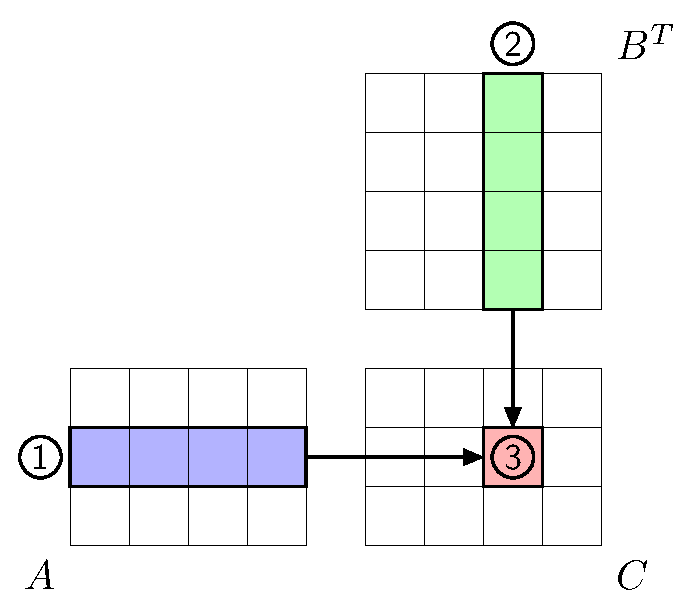
\includegraphics[width=\textwidth]{HLPP/allpairs_access_pattern}
    \caption{}
    \label{fig:allpairs:access:transposed}
  \end{subfigure}
  \caption{The allpairs computation schema. (\subref{fig:allpairs:access:not_transposed}): element $C_{2,3}$
    \protect\tikz[baseline=(char.base)]\protect\node[shape=circle,draw,inner sep=1pt] (char) {3};
    is computed by combining the second row of $A$
    \protect\tikz[baseline=(char.base)]\protect\node[shape=circle,draw,inner sep=1pt] (char) {1};
    with the third row of $B$
    \protect\tikz[baseline=(char.base)]\protect\node[shape=circle,draw,inner sep=1pt] (char) {2};
    using the binary operator $\oplus$. (\subref{fig:allpairs:access:transposed}): the same situation where the transpose of matrix $B$ is shown.}
  \label{fig:allpairs:access}
\end{figure}

Let us consider two example applications which can be expressed by customizing the \allpairs skeleton with a particular function $\oplus$.

\paragraph{Example 1:}
The Manhattan distance (or $L_1$ distance) is a measure of distance which is used in many applications.
In general, it is defined for two vectors, $x$ and $y$, of equal length $d$, as follows:
\begin{equation}
  \label{eq:man_dist}
  \ManDist\ x\ y = \sum_{k=1}^d | x_k - y_k |
\end{equation}
In~\cite{ChangDeQuRo2009}, the so-called Pairwise Manhattan Distance (\emph{PMD}) is studied as a fundamental operation in hierarchical clustering for data analysis.
\emph{PMD} is obtained by computing the Manhattan distance for every pair of rows of a given matrix.
This computation for arbitrary matrix $A$ can be expressed using the \allpairs skeleton customized with the Manhattan distance defined in \autoref{eq:man_dist}:
\begin{equation}
  \PMD\ A = allpairs\ \mbox{\emph{ManDist}}\ A\ A
\end{equation}
The $n\times n$ matrix computed by the customized skeleton contains the Manhattan distance for every pair of rows of the input $n\times d$ matrix $A$.

\paragraph{Example 2:}
Matrix-matrix multiplication is a basic linear algebra operation, which is a building block of many scientific applications.
A $n\times d$ matrix $A$ is multiplied with a $d\times m$ matrix $B$, producing a $n\times m$ matrix $C=A\times B$ whose element $C_{i,j}$ is computed as the dot product of the $i$th row of $A$ with the $j$th column of $B$.
The dot product of two vectors, $a$ and $b$ of length $d$, is computed as follows:
\begin{equation}
  \dotProduct\ a\ b = \sum_{k=1}^d a_k \cdot b_k
\end{equation}
The matrix multiplication can be expressed using the \allpairs skeleton as:
\begin{equation}
  A\times B = allpairs\ \dotProduct\ A\ B^T
  \label{eq:mat_mult_allpairs}
\end{equation}
where $B^T$ is the transpose of matrix $B$.

% TODO: moved to impl ...
% \paragraph{The \allpairs skeleton using multiple GPUs}
% \label{sec:allpairs:multi_gpu}
% \begin{figure}[b]
%   \centering
%   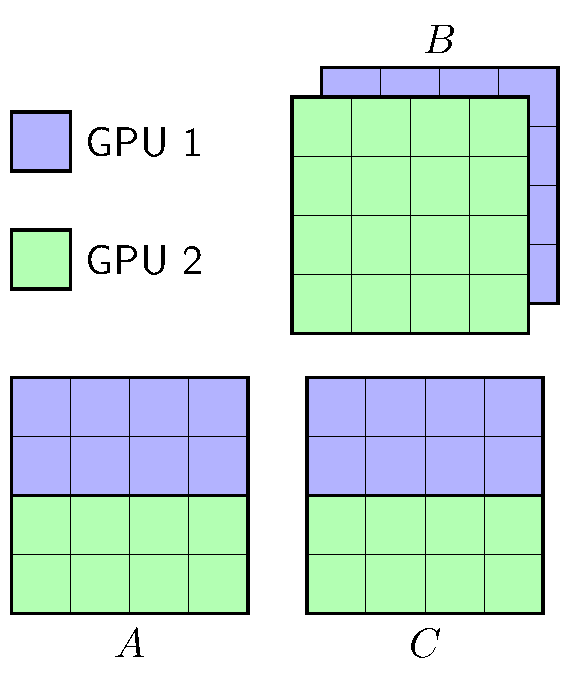
\includegraphics[width=.3\textwidth]{HLPP/multi_gpu}
%   \caption{Data distributions used for a system with two GPUs: matrices $A$ and $C$ are \emph{block} distributed, matrix $B$ is \emph{copy} distributed.}
%   \label{fig:multi_gpu}
% \end{figure}
% 
% The \allpairs skeleton can be efficiently implemented not only on systems with a single \GPU, but on multi-\GPU systems as well.
% The necessary data distribution can be easily expressed using two of \SkelCL's \emph{distributions}, as shown in \autoref{fig:multi_gpu}:
% Matrix $B$ is \emph{copy} distributed, \ie, it is copied entirely to all \GPUs in the system.
% Matrix $A$ and $C$ are \emph{block} distributed, \ie, they are row-divided into as many equally-sized blocks as \GPUs are available;
% each block is copied to its corresponding \GPU.
% Following these distributions, each \GPU computes one block of the result matrix $C$.
% In the example with two GPUs shown in \autoref{fig:multi_gpu}, the first two rows of $C$ are computed by \GPU 1 and the last two rows by \GPU 2.
% The \allpairs skeleton automatically selects these distributions, therefore, the same source code can be used when using a single \GPU or multiple \GPUs.



\subsubsection{The specialized \allpairs skeleton}
\label{sec:opt_allpairs_skeleton}
When targeting \GPU architectures, implementing an optimized version of the \allpairs skeleton is possible if certain assumptions about the customizing function $f$ can be made.
In this section, we will start by discussing the properties of $f$ necessary for an optimized \GPU implementation.
In particular we will analyze the memory access pattern of the matrix multiplication as the memory accesses turns out to be crucial for the performance.
We then observe that the identified memory access pattern can also be found in other allpairs computations and, therefore, define a specialized version of the allpairs skeleton, which is suitable for applications having this pattern.
% Finally, we estimate the gained efficiency by the optimized implementation over the generic one.


\paragraph{The memory access pattern of the matrix multiplication}
\begin{figure}[t]
  \centering
  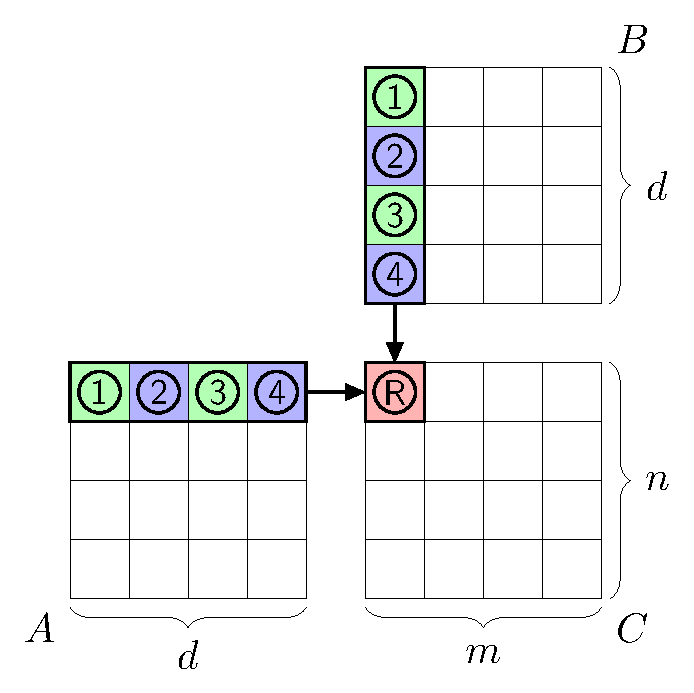
\includegraphics[width=0.4\textwidth]{HLPP/single_memory_access}
  \caption{The memory access pattern of the matrix multiplication $A\times B = C$.}
  \label{fig:mm_access_pattern}
\end{figure}
Figure~\ref{fig:mm_access_pattern} shows the memory access pattern of the matrix multiplication for $4\times 4$ matrices.
To compute the element \circled{R} of the result matrix $C$, the first row of matrix $A$ and the first column of matrix $B$ are combined.
In the skeleton-based code, these two vectors are used by the customizing function $f$, which is the dot product in case of the matrix multiplication.
The dot product performs a pairwise multiplication of the two vectors and then sums up the intermediate result.
In the example, the two elements marked as \circled{1} are multiplied first and the intermediate result is stored;
then, the next elements (marked as \circled{2}) are multiplied and the result is added to the intermediate result, and so forth.
% TODO: Moved to impl section ...
% Let us assume targeting \GPU architectures and estimate the number of global (and therefore expensive) memory accesses required for computing an element of the matrix multiplication in the generic case.
% One global memory read access for every element of both input vectors is performed, and a single global memory write access is required to write the result into the output matrix.
% Therefore, 
% \begin{equation}
%   n\cdot m\cdot (d + d + 1)
%   \label{eq:mm:accesses}
% \end{equation}
% global memory accesses are performed in total, where $n$ and $m$ are the height and width of matrix $C$ and $d$ is the width of $A$ and the height of $B$.
% By using the fast but small local memory this number of global memory accesses can be reduces and, thus, performance can be improved.
% Using the local memory for matrix matrix multiplication is a well known optimization.

A key observation is, that other applications share the same memory access pattern as the matrix multiplication shown in \autoref{fig:mm_access_pattern}.
For example, the customizing function of the pairwise Manhattan distance as defined by \autoref{eq:man_dist} follows obviously the same memory access pattern as the matrix multiplication.
To find a common representation for a customizing function with this pairwise access pattern, we describe it as a sequential composition of two basic algorithmic skeletons: \zip and \reduce.
% The \emph{sequential composition} composition of two functions (or skeletons) $f$ and $g$ is denoted by $g \circ f$ which means that $f$ is applied first and then $g$ is applied to the result value of $f$ as input, \ie, $(g\circ f)\ x = g(f\ x)$.

For the \reduce skeleton customized with $\oplus$ and corresponding identity element \id, and the \zip skeleton customized with $\otimes$ we can sequentially compose them as follows:
\begin{eqnarray*}
  \reduce\ (\oplus)\ \id\ \big(\ \zip\ (\otimes)\ a\ b\ \big) &=&\\
  \reduce\ (\oplus)\ \id\ \big(\ \zip\ (\otimes)\ \DottedVector{a_1}{a_n}\ \DottedVector{b_1}{b_n}\ \big) &=&\\
  (a_1 \otimes b_1)\ \ \oplus &\cdots& \oplus\ \ (a_n \otimes b_n)
\end{eqnarray*}

This composition of the two customized skeletons yields a function which we denote \zipReduce; it takes two input vectors and produces a single scalar value:

\begin{equation*}
  \zipReduce\ (\oplus)\ \id\ (\otimes)\ a\ b \eqdef 
  \reduce\ (\oplus)\ \id\ \big(\ \zip\ (\otimes)\ a\ b\ \big)
\end{equation*}

Following the definition of \zipReduce, we can express the customizing function of the Manhattan distance as follows.
We use the binary operator $a \ominus b = |a - b|$ as the customizing function for \zip, and addition as the customizing function for the \reduce skeleton:
\begin{eqnarray*}
    \ManDist\ a\ b &=& \sum_{i=1}^{n} | a_i - b_i | = (a_1 \ominus b_1) + \cdots + (a_n \ominus b_n)\\
    &=& \zipReduce\ (+)\ 0\ (\ominus)\ \DottedVector{a_1}{a_n}\ \DottedVector{b_1}{b_n}
\end{eqnarray*}

Similarly, we can express the dot product (which is the customizing function of matrix multiplication) as a \zip-\reduce composition, by using multiplication for customizing the \zip skeleton and addition for customizing the \reduce skeleton:
\begin{eqnarray*}
  \dotProduct\ a\ b &=& \sum_{i = 1}^{n} a_i \cdot b_i = (a_1 \cdot b_1) + \cdots + (a_n \cdot b_n)\\
  &=& \zipReduce\ (+)\ 0\ (\times)\ a\ b
\end{eqnarray*}

\paragraph{Definition of the specialized \allpairs skeleton}

We can now specialize the generic Definition~\autoref{def:allpairs} of the \allpairs skeleton by employing the sequential composition of the customized \reduce and \zip skeletons for customizing the \allpairs skeleton.
From here on, we refer to this specialization as the \allpairs skeleton \emph{customized with \zip-\reduce}.

\begin{definition}
  \label{def:allpairs:specialized}
  Let $A$ be a $n\times d$ matrix, $B$ be a $m\times d$ matrix, and $C$ be a $n\times m$ matrix, with their elements $a_{i,j}$, $b_{i,j}$, and $C_{i,j}$ respectively.
  Let $\oplus$ be an associative binary customizing operator with the corresponding identity element \id.
  Let $\otimes$ be a binary customizing operator.
  The specialized algorithmic skeleton \allpairs customized with \zip-\reduce is defined as follows:
  \begin{equation*}
    \begin{split}
      \allpairs\ (\oplus)\ \id\ (&\otimes)\ %
      \left[ \begin{array}{c} a_{1,1} \cdots a_{1,d}\\[.25em] \vdots \hspace{4em} \vdots\\[.25em] a_{n,1} \cdots a_{n,d} \end{array}\right]\ %
      \left[ \begin{array}{c} b_{1,1} \cdots b_{1,d}\\[-.25em] \cdot \hspace{4em} \cdot\\[-.75em] \cdot \hspace{4em} \cdot\\[-.25em] b_{m,1} \cdots b_{m,d} \end{array}\right]%
      \\
    &\eqdef \left[ \begin{array}{ccc} C_{1,1} & \cdots & C_{1,m}\\[.25em] \vdots & & \vdots\\[.25em] C_{n,1} & \cdots & C_{n,m} \end{array} \right]
    \end{split}
  \end{equation*}
  where elements $C_{i,j}$ of the $n\times m$ matrix $C$ are computed as follows:
  \[
    C_{i,j} = \zipReduce\ (\oplus)\ \id\ (\otimes)\ \DottedVector{a_{i,1}}{a_{i,d}}\ \DottedVector{b_{j,1}}{b_{j,d}}
  \]
\end{definition}


While not every allpairs computation can be expressed using this specialization, many real-world problems can.
In addition to the matrix multiplication and the pairwise Manhattan distance examples are the pairwise computation of the Pearson correlation coefficient~\cite{ChangDeQuRo2009} and estimation of Mutual Informations~\cite{DaubStSeKl2004}.
The composition of \zip and \reduce is well known in the functional programming world.
Google's popular \emph{MapReduce} programming model has been inspired by a similar composition of the \map and \reduce skeletons.
\cite{Laemmel2007} extensively discusses the relation of MapReduce to functional programming.


% TODO: Moved to impl ...
% \paragraph{Estimation of the performance gain of specialization}
% By expressing the customizing function of the \allpairs skeleton as a \zip-\reduce composition, we provide additional semantic information about the memory access pattern of the customizing function to the skeleton implementation, thus allowing for improving the performance.
% Our idea of optimization is based on the OpenCL programming model that organizes \emph{work-items} (i.\,e., threads executing a kernel) in \emph{work-groups} which share the same \GPU local memory.
% By loading data needed by multiple work-items of the same work-group into the local memory, we can avoid repetitive accesses to the global memory.
% 
% \begin{figure}[b]
%   \centering
%   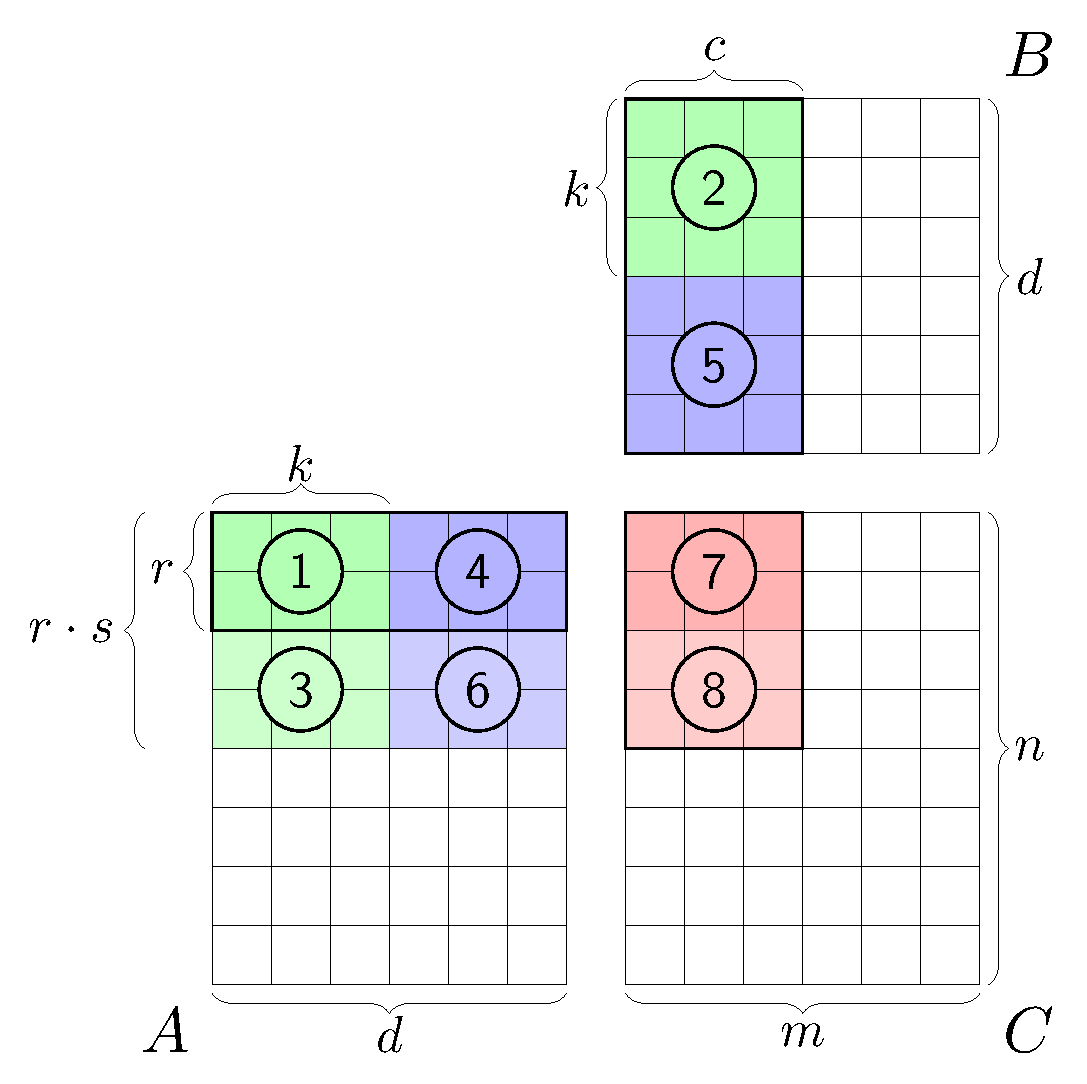
\includegraphics[width=.4\textwidth]{HLPP/memory_access}
%   \caption{Implementation schema of the specialized allpairs skeleton.}
%   \label{fig:memory_access}
% \end{figure}
% For the \allpairs skeleton with the \zip-\reduce customizing function, we can adopt the implementation schema for \GPUs~\cite{SarjeAl2013}, as shown in Figure~\ref{fig:memory_access}.
% We allocate two arrays in the local memory, one of size $r\times k$ ($r=2$, $k=3$ in Figure~\ref{fig:memory_access}) for elements of $A$ and one of size $k\times c$ ($c=3$ in Figure~\ref{fig:memory_access}) for elements of $B$.
% A work-group consisting of $c\times r$ work-items computes $s$ blocks ($s=2$ in Figure~\ref{fig:memory_access}) of the result matrix $C$.
% In Figure~\ref{fig:memory_access}, the two blocks marked as \circled{7} and \circled{8} are computed by the same work-group as follows.
% In the first iteration, the elements of blocks \circled{1} and \circled{2} are loaded into the local memory and combined following the \zip-\reduce pattern.
% The obtained intermediate result is stored in block \circled{7}.
% Then, the elements of block \circled{3} are loaded and combined with the elements from \circled{2} which still reside in the local memory.
% The intermediate result is stored in block \circled{8}.
% In the second iteration, the algorithm continues in the same manner with blocks \circled{4}, \circled{5}, and \circled{6}, but this time, the elements of the blocks are also combined with the intermediate results of the first iteration, which are stored in blocks \circled{7} and \circled{8}.
% The advantage of computing multiple blocks by the same work-group is that we keep the elements of $B$ in the local memory when computing the intermediate results, \ie, we do not reload block \circled{2} twice for the computation of blocks \circled{7} and \circled{8}.
% 
% Every element loaded from the global memory is used by multiple work-items:
% \eg, the upper left element of block \circled{1} is loaded only once from the global memory, but used three times:
% in the computation of the upper left, upper middle, and upper right elements of \circled{7}.
% In general, every element loaded from $A$ is reused $c$ times, and every element from $B$ is reused $r\cdot s$ times.
% As the intermediate results are stored in the global memory of matrix $C$, we perform two additional memory accesses (read/write) for every iteration, \ie, $2\cdot \frac{d}{k}$ in total.
% Therefore, instead of $n\cdot m\cdot (d + d + 1)$ (see \autoref{eq:mm:accesses}) global memory accesses necessary when using the non-specialized skeleton and, thus, only the global memory, only
% \begin{equation}
%   n\cdot m\cdot (\frac{d}{r\cdot s} + \frac{d}{c} + 2\cdot \frac{d}{k})
% \end{equation}
% global memory accesses are performed.
% By increasing the parameters $s$ and $k$, or the number of work-items in a work-group ($c$ and $r$), more global memory accesses can be saved.
% However, the work-group size is limited by the \GPU hardware.
% While the parameters can be chosen independently of the matrix sizes, we have to consider the amount of available local memory.
% \cite{Friese2013}~and~\cite{SarjeAl2013}~discusses how suitable parameters can be found by performing runtime experiments.
% In~\cite{Friese2013} the parameters $c = 32$, $r=8$, $s=32$, and $k=64$ are used on modern \GPU hardware showing good performance.
% 
% We will report measurements of the performance difference for the two skeleton implementations on real hardware in \autoref{chapter:skelcl:apps}.
% 
% 




% ============================================================================ %
% ============================================================================ %
\section{The \SkelCL Library}
\label{section:skelcl-library}
In this section we discuss the \SkelCL library -- our implementation of the \SkelCL programming model.
It provides a \Cpp~\API that implements the features of the \SkelCL programming model, and thus liberates the application developer from writing low-level code.
In addition, the library provides some commonly used utility functions, \eg, for program initialization.
The \SkelCL library is open source software and available at: \url{http://skelcl.uni-muenster.de}.

We start our discussion with an example showing how to use the \SkelCL library.
We describe the syntax used to represent the \SkelCL programming model introduced in the previous section.
This will include a discussion of \Cpp techniques used to implement the library.
We then shift the focus to the implementations of the memory management, algorithmic skeletons, and distributions.










\subsection{Programming with the \SkelCL Library}

\autoref{lst:skelcl:dotproduct} shows the implementation of the dot product computation, discussed in the previous section, in \SkelCL.
After including the appropriate \SkelCL headers (\autoref{lst:skelcl:dotproduct:inc:start}---\autoref{lst:skelcl:dotproduct:inc:end}) the \SkelCL library can be initialized as shown in \autoref{lst:skelcl:dotproduct:init}.
This will perform the initializations required by \OpenCL.
The argument provided to the \code{init} function specifies how many and which \OpenCL devices should be used by \SkelCL.
Here a single device should be used which can be of any type, \ie, it can be either a \CPU or a \GPU.
The dot product is specified using the \zip and \reduce skeletons.
The skeletons are created using \code{zip} (\autoref{lst:skelcl:dotproduct:zip}) and \code{reduce} (\autoref{lst:skelcl:dotproduct:reduce}) functions which expect the customizing functions of the skeletons as arguments.
In this example we use \Cpp lambda expressions (\autoref{lst:skelcl:dotproduct:zip:lambda} and \autoref{lst:skelcl:dotproduct:reduce:lambda}) to specify the customizing functions of the skeletons.
We create the two input \code{Vector}s from C style pointers (\autoref{lst:skelcl:dotproduct:vecAB}).
In \autoref{lst:skelcl:dotproduct:apply} we perform the computation by applying the customized skeletons to the data, before we finally return the computed result in \autoref{lst:skelcl:dotproduct:return}.

\begin{lstlisting}[%
caption={Implementation of the dot product computation in \SkelCL.},%
float=t,%
numbers=left,%
label={lst:skelcl:dotproduct}]
#include <SkelCL/SkelCL.h>$\label{lst:skelcl:dotproduct:inc:start}$
#include <SkelCL/Zip.h>
#include <SkelCL/Reduce.h>
#include <SkelCL/Vector.h>$\label{lst:skelcl:dotproduct:inc:end}$

float dotProduct(const float* a, const float* b, int n) {
  using namespace skelcl;
  skelcl::init( 1_device.type(deviceType::ANY) );$\label{lst:skelcl:dotproduct:init}$

  auto mult = zip([](float x, float y) { return x*y; });$\label{lst:skelcl:dotproduct:zip}$$\label{lst:skelcl:dotproduct:zip:lambda}$
  auto sum = reduce([](float x, float y){ return x+y; }, 0);$\label{lst:skelcl:dotproduct:reduce}$$\label{lst:skelcl:dotproduct:reduce:lambda}$

  Vector<float> A(a, a+n); Vector<float> B(b, b+n);$\label{lst:skelcl:dotproduct:vecAB}$

  Vector<float> C = sum( mult(A, B) );$\label{lst:skelcl:dotproduct:apply}$

  return C.front();$\label{lst:skelcl:dotproduct:return}$
}
\end{lstlisting}

\autoref{lst:skelcl:dotproduct} shows that the \SkelCL library integrates nicely with \Cpp:
the interface of the \code{Vector} class looks familiar to \Cpp programmers and the usage of modern \Cpp features like lambda expressions, type deduction (\code{auto}), and user-defined literals simplify the programming as functions can be defined directly inline, type information can be omitted, and the specification of which devices to use can be written intuitively.

We will now discuss how our implementation enables this comfortable level of integrating \SkelCL with \Cpp.










\subsection{Syntax and Integration with \Cpp}
\label{section:skelcl-library:syntax}

The \SkelCL library is built on top of \OpenCL.
This offers clear benefits as well as introduces technical challenges.
One of the technical challenges is, that \OpenCL requires the kernel to be specified as a string in the host program.
While this enables portability across different hardware architectures, it also introduces a burden on the application developer as strong typing cannot be guaranteed statically when the host program is compiled.
For the implementation of \SkelCL, we choose to address this issue using a two-step implementation.
In the first step, a custom compiler transforms the source code as seen in \autoref{lst:skelcl:dotproduct} to a representation where the kernel computations are represented as strings as required by \OpenCL.
In the second step, the transformed program is compiled using a traditional \Cpp compiler to produce the final executable.

This allows ourselves to free the users from writing strings in their application code and maintain the usual type safety guarantees from \Cpp at compile time.
Furthermore, we implemented type inference capabilities in our source-to-source compiler to free the application developer from specifying type information explicitly.
Our two-step design also allows application developers to compile their application code into a form which then can be deployed on systems where it might be difficult to install a custom compiler.

In the next paragraph, we will start the discussion of our source-to-source compiler.
We will discuss how our custom compiler, together with our template-based implementation, helps to maintain strong type safety at compile time.
Finally, we will look at issues regarding the integration with \Cpp like sharing code between host and device code.

\paragraph{The custom SkelCL compiler}
To allow a deep integration of \SkelCL code with \Cpp, we implemented a custom compiler: \code{skelclc}.
We leverage the LLVM infrastructure~\cite{Lattner2004} for building this compiler.
LLVM and the related Clang project offer well-defined application programming interfaces for writing C and \Cpp related compiler tools.
In particular the \emph{LibTooling} \API allows for writing tools which search for particular patterns in the abstract syntax tree (AST) which is representing the source code and perform actions on the found code fragments.
The \code{skelclc} custom compiler does exactly this.
For example, the custom compiler searches for an expression like this:
\begin{lstlisting}[numbers=none,label={lst:skelclc:before},caption={\SkelCL code snippet before transformation.}]
auto mult = zip( [](float x, float y){ return x*y; } );
\end{lstlisting}
and replaces it with:
\smallskip
\begin{lstlisting}[numbers=none,label={lst:skelclc:after},caption={\SkelCL code snippet after transformation.}]
auto mult = Zip<Container<float>(Container<float>,
                                 Container<float>)>(
              Source("float func(float x, float y)"
                     " { return x*y; }"), "func");
\end{lstlisting}

In this example, the \code{zip} function has been transformed into a call of the constructor of the \code{Zip} class and the lambda expression has been transformed into a string.
Furthermore, type information that has been inferred from the lambda expression, has been added to the templated \code{Zip} class.

The user is free to write the expression in \autoref{lst:skelclc:after} explicitly, but it is arguably more convenient to write the expression as in \autoref{lst:skelclc:before} and let \code{skelclc} perform the transformation automatically.

For every skeleton available in \SkelCL, there exists a function like \code{zip} which is transformed by \code{skelclc} to a call of the constructor of the corresponding skeleton class.

\paragraph{Maintaining type safety}
Each skeleton is represented by a templated class, as seen in \autoref{lst:skelclc:after} for the \zip skeleton.
The template arguments of the skeleton define the types which can be used when executing the skeleton.
For a skeleton of type \code{skeleton<T(U)>}, an object of type \code{U} has to be provided on execution to receive an object of type \code{T}.
In this respect skeletons behave exactly like functions in \Cpp which can be represented using the \code{std::function<T(U)>} template class.
Skeletons taking more then one argument (like the \code{zip} skeleton) are represented as \code{skeleton<T(U, V)>}.% using the \emph{variadic template} feature of \Cpp.

When performing the transformations, \code{skelclc} infers the types used as template arguments of the skeleton class.
To do so, it determines the types of the lambda expression arguments and skeleton's result type.
For \autoref{lst:skelclc:before} this is: \code{float} and \code{float} as argument types and \code{float} as the result type.
The result type is inferred following standard \Cpp rules.
Based on these types, the template arguments of the skeleton are constructed.

The skeletons \map, \zip, and \stencil can operate on either \code{Vector} or \code{Matrix}.
For each of these skeletons there exist three kinds of factory functions:
1)~for creating a skeleton operating on vectors, \eg, \code{mapVector};
2)~for creating a skeleton operating on matrices, \eg, \code{mapMatrix};
3)~for creating a skeleton capable of operating on both vectors and matrices, \eg, \code{map}.
To allow the latter case, the templated class \code{Container} was introduced.
Using the template specialization mechanism, the mentioned skeletons have a special implementation when \code{Container} is used as a template argument.
In this case, the classes provide a templated function call operator which can be used either with \code{Vector} or \code{Matrix}.

Type safety is guaranteed, as the templated skeleton classes can only be executed with a container of compatible type and the type inference ensures that the user function has exactly the same type as the template argument of the skeleton class.
Therefore, applying the user function to the input data is always a type-safe operation.

Because skeletons are strongly typed, the composition of skeletons is type-safe as well, \ie, in \autoref{lst:skelcl:dotproduct} type safety between the two skeletons is guaranteed.
If the result type of \code{zip} does not match the input type of \code{reduce}, a compile time error would occur.

\paragraph{Integration with \Cpp}
To allow a deep integration with \Cpp, a customizing function is allowed to make use of user-defined types and make calls to other functions.
The \code{skelclc} compiler detects these behaviors and ensures that the definition of the user defined type and the source code of all called functions is included in the source code passed to the skeleton.
This frees the user from providing type definitions and source code twice, which would be required when using \OpenCL directly or using \SkelCL without the \code{skelclc} compiler.
Code duplication should almost always be avoided as it can easily lead to hardly maintainable code and subtle bugs.

\paragraph{Additional Arguments:}
In real-world applications (\eg, the LM OSEM discussed in detail in \autoref{section:medical-imaging}), user-defined functions often operate not only on a skeleton's input vector, but may also take additional inputs.
With only a fixed number of input arguments, traditional skeletons would not be applicable for the implementation of such applications.
In \SkelCL, skeletons can accept an arbitrary number of additional arguments which are passed to the skeleton's customizing function.

\autoref{lst:saxpy:addArgs} shows an example implementation in \SkelCL of the \emph{single-precision real-alpha x plus y} ($saxpy$) computation -- a commonly used \BLAS routine.
\begin{lstlisting}[%
  caption={The \BLAS $saxpy$ computation using the \zip skeleton with additional arguments},%
  float=tbp,%
  label={lst:saxpy:addArgs}]
float a = initScalar();

/* create skeleton Y <- a * X + Y */
auto saxpy = zip(
      [](float x, float y, float a) { return a*x+y; } );$\label{lst:saxpy:addArgs:arg}$

Vector<float> X(SIZE); initVector(X);
Vector<float> Y(SIZE); initVector(Y);

Y = saxpy( X, Y, a );      /* execute skeleton */ $\label{lst:saxpy:addArgs:execution}$
\end{lstlisting}
The $saxpy$ computation is a combination of scalar multiplication of $a$ with vector $\vec{x}$ followed by vector addition with $\vec{y}$.
In \autoref{lst:saxpy:addArgs}, the computation is implemented using the \zip skeleton:
vectors $\vec{x}$ and $\vec{y}$ are passed as input, while factor $a$ is passed to the customizing function as an additional argument (\autoref{lst:saxpy:addArgs:arg}).
The additional argument is simply appended to the argument list when the skeleton is executed (\autoref{lst:saxpy:addArgs:execution}).
Besides scalar values, like shown in the example, vectors and matrices can also be passed as additional arguments to a skeleton.
When vectors or matrices are used as additional arguments, the user is responsible to ensure that no race conditions occur when writing to or reading from the container.
If the container is only used for reading, it is guaranteed that no race conditions will occur.

The additional argument feature is implemented in \SkelCL using the variadic template feature from \Cpp.

\paragraph{Lambda captures:}
In \Cpp, lambda expressions can make use of variables which have been accessible at the time the lambda expression is created.
The user has to explicitly indicate how these variable are \emph{captured}, \ie, how they will be accessed once the lambda is executed.
A variable can either be captured \emph{by-value} or \emph{by-reference}.
If a variable is captured by-value, a copy of the variable is made at the time the lambda expression is created and accessed later when the lambda expression is executed.
If a variable is captured by-reference, the original variable is accessed when the lambda expression is executed through a reference.
Capturing a variable by reference allows the user to change the content of the variable from inside the lambda expression, furthermore, in a parallel setting the user has to ensure that the lifetime of the variable exceeds the time when the lambda expression is executed.

In \SkelCL, the customizing function can be expressed as a lambda expression capturing variables.
The by-value capturing of variables is fully supported by the \code{skelclc} compiler and the capturing by-reference is supported with the following restrictions:
by-reference capturing is only allowed if the reference is used to read from the variable only, and writing to the captured variable is forbidden.
The reason for these restrictions is that when executing the lambda expression on the \GPU, a write to a by-reference captured variable requires a costly data transfer to ensure that the variable stored in \CPU memory is modified.
Furthermore, as the lambda expression will be executed multiple times in parallel as part of the skeletons execution, it is likely that race conditions occur when writing to the captured reference.
We can rewrite the $saxpy$ example using a lambda expression capturing the variable $a$ as shown in \autoref{lst:saxpy:capture}.
\begin{lstlisting}[%
  caption={[The \BLAS $saxpy$ computation using a \zip skeleton customized with a lambda expression capturing a variable.]
           The \BLAS $saxpy$ computation using a \zip skeleton customized with a lambda expression capturing the variable $a$.},%
  float=tbp,%
  label={lst:saxpy:capture}]
float a = initScalar();

/* create skeleton Y <- a * X + Y */
auto saxpy = skelcl::zip(
      [a](float x, float y) { return a*x+y; }); $\label{lst:saxpy:capture:capture}$

Vector<float> X(SIZE); initVector(X);
Vector<float> Y(SIZE); initVector(Y);

Y = saxpy( X, Y );      /* execute skeleton */ $\label{lst:saxpy:capture:execute}$
\end{lstlisting}

The variable $a$ is now captured by the lambda expression in \autoref{lst:saxpy:capture:capture}.
Note that $a$ is no longer passed as an argument when executing the skeleton in \autoref{lst:saxpy:capture:execute}.

\vspace{1em}

Additional arguments and lambda captures are related techniques which both can be used to make additional data available inside of the user function.
There is one main technical differences between both:
for using lambda captures the variable to be captured has to be declared and available when \emph{declaring} the user function (in \autoref{lst:saxpy:capture:capture} in \autoref{lst:saxpy:capture}) which is not the case for the additional argument feature where the variable has to available when \emph{executing} the skeleton (in \autoref{lst:saxpy:addArgs:execution} in \autoref{lst:saxpy:addArgs}).
By supporting the capturing feature of lambda expressions \SkelCL source code becomes more \Cpp idiomatic, but ultimately the user has the choice of using either feature as it fits his or her needs and personal taste.








\subsection{Skeleton Execution on \OpenCL Devices}
\label{section:skelcl-library:execution}
The process of executing a skeleton on an \OpenCL device, \eg, a \GPU, follows always the same steps independently of the skeleton involved.
This process is described in this subsection, before we will look at the individual skeleton implementations in the next subsection.

The \code{skelclc} compiler transforms the \SkelCL application code so that the source code of the customizing function of a skeleton is available to the \SkelCL library implementation as a string.
When a skeleton instance is created, the \SkelCL library implementation performs the following steps to create an \OpenCL kernel:
1)~the source code of the customizing function is merged with the \OpenCL kernel implementation of the skeleton;
2)~the merged source code is adapted into the final \OpenCL kernel. This is done to support additional arguments and so that names and types of the customizing function and skeleton implementation match;
3)~the created \OpenCL kernel is stored to a file to avoid performing steps 1) and 2) multiple times for the same kernel.

On execution of the skeleton, the following steps are performed to execute the computation on an \OpenCL device:
1)~the data of the input containers is uploaded to the \OpenCL device, if it is not already there;
2)~the \OpenCL kernel arguments are set, including the additional arguments;
3)~the \OpenCL kernel is executed.

In the next two paragraphs, we will describe these two processes and their individual steps.

\paragraph{Creating an OpenCL kernel}
We will use the $saxpy$ example from the previous section as a running example to explain how an \OpenCL kernel is created.
\autoref{lst:saxpy:transformed} shows the code for the $saxpy$ application emitted by the \code{skelclc} compiler after receiving the code shown in \autoref{lst:saxpy:addArgs} as input.
\begin{lstlisting}[%
  caption={Source code for the $saxpy$ application emitted by the \code{skelclc} compiler.},%
  float=tbp,%
  label={lst:saxpy:transformed}]
float a = initScalar();
/* create skeleton Y <- a * X + Y */
auto saxpy = skelcl::Zip<Vector<float>(Vector<float>,
                                       Vector<float>,
                                       float)>(
     skelcl::Source("float func(float x, float y, float a)"$\label{lst:saxpy:transformed:funcStart}$
                    " { return a*x+y; }"), "func"); $\label{lst:saxpy:transformed:funcEnd}$
/* create input vectors */
Vector<float> X(SIZE); initVector(X);
Vector<float> Y(SIZE); initVector(Y);
Y = saxpy( X, Y, a );      /* execute skeleton */
\end{lstlisting}

To create the corresponding \OpenCL kernel, the source code of the customizing function in \autoref{lst:saxpy:transformed:funcStart} and \autoref{lst:saxpy:transformed:funcEnd} is combined with the prototype implementation of the \zip skeleton which is shown in \autoref{lst:zip:impl}.
%
\begin{lstlisting}[%
  caption={Prototype implementation of the \zip skeleton in \OpenCL.},%
  float=tbp,%
  label={lst:zip:impl}]
typedef int T0; typedef int T1; typedef int T2;$\label{lst:zip:impl:typedef}$

kernel void ZIP(const global T0* left,
                const global T1* right,
                      global T2* out,
                const unsigned int size) {
  unsigned int id = get_global_id(0);
  if (id < size) { $\label{lst:zip:impl:boundaryCheck}$
    out[id] = USER_FUNC(left[id], right[id]); } }  $\label{lst:zip:impl:call}$
\end{lstlisting}
%
The prototype implementation created the \OpenCL kernel \code{ZIP} receiving three pointers to global memory and one integer as arguments.
A boundary check is performed in \autoref{lst:zip:impl:boundaryCheck} before a function with the name \code{USER\_FUNC} is called (\autoref{lst:zip:impl:call}) with a pair of elements read from the two input arrays \code{left} and \code{right}.
The result of the function call is stored in the output array \code{out}.

The combined source codes clearly do not yet form a valid \OpenCL kernel as there exists no function called \code{USER\_FUNC}.
This \emph{prototype} implementation has to be adapted to become a valid \OpenCL kernel.
To make this adaption, the \SkelCL library implementation makes use of the same LLVM and Clang infrastructure used to build the \code{skelclc} compiler.
Three steps are performed to create a valid \OpenCL kernel:
1)~the customizing function is renamed into \code{USER\_FUNC};
2)~the types of the customizing functions are used to change the \code{typedef}s in \autoref{lst:zip:impl:typedef} so that the types of the kernel function \code{ZIP} match;
3)~the additional arguments of the customizing function are appended to the parameter list of the kernel function \code{ZIP} and the call to the customizing function is adapted to forward the arguments.

After these steps the source code has been transformed into a valid \OpenCL kernel as shown in \autoref{lst:zip:mergedImpl}.
\begin{lstlisting}[%
  caption={\OpenCL implementation of the \zip skeleton customized for performing the $saxpy$ computation.},%
  float=tbp,%
  label={lst:zip:mergedImpl}]
float USER_FUNC(float x, float y, float a) { return a*x+y; }
typedef float T0; typedef float T1; typedef float T2;

kernel void ZIP(const global T0* left,
                const global T1* right,
                      global T2* out,
                const unsigned int size, float a) {
  unsigned int id = get_global_id(0);
  if (id < size) {
    out[id] = USER_FUNC(left[id], right[id], a); } }
\end{lstlisting}

Performing the adaption of the source code involves parsing the code and building an abstract syntax tree for it by the Clang compiler library.
Performing this every time a skeleton is created is wasteful as this task can take up to several hundreds of milliseconds, which can be a considerable overhead for small kernels.
Therefore, the \SkelCL library implements a caching of already transformed kernels to disk.
If the same kernel is used again, the transformed code is loaded from the cache.%
\footnote{We observed that loading kernels from disk is in some cases at least five times faster than creating them from the source.}


\paragraph{Execute a Skeleton on an OpenCL Device}
On execution of the skeleton, the created \OpenCL kernel is executed on possibly multiple \OpenCL devices.
The data distribution of the input containers determine which \OpenCL devices are used for the execution.
If the copy, block, or overlap distribution is used, this means that all available devices are involved in the computation as defined by the distributions.
If the single distribution is used then just a single device is used.
If no distribution is set for the input containers, each skeleton selects a default distribution.

The first step for the execution is to upload the data of the input containers to the \OpenCL devices.
Before performing a data transfer, the \SkelCL implementation checks if the transfer is necessary or if the data is already up to date on the receiving side.
The details how this is implemented in the memory management part of \SkelCL are described in \autoref{section:skelcl-library:memory-management}.

Before enqueuing the \OpenCL kernel in the \OpenCL command queue, its kernel arguments have to be set.
First, the regular arguments are set correspondingly to the order of arguments as defined in the skeleton's prototype implementation of the \OpenCL kernel.
Afterwards, the additional arguments are set.

Finally, the \OpenCL kernel is enqueued with a global size corresponding to the size of the input containers.










\subsection{Algorithmic Skeleton Implementations}
\label{section:skelcl-library:skeletons}
The \SkelCL library implements each skeleton of the \SkelCL programming model using one or more \OpenCL kernels.
In this subsection, we discuss the implementation of each skeleton targeting single- and multi-device systems.





\subsubsection{The Map Skeleton}
The \OpenCL kernel implementing the \map skeleton is straightforward and similar to the implementation of the \zip skeleton shown in \autoref{lst:zip:impl}.
After a boundary check is performed, the customizing function is called with an item of the input container.
The return value is stored in the output container.
On execution, the size of the input container determines the number of work-items launched for executing the kernel code.
The same kernel code is used on single- and multi-device systems.
If the input container has no distribution declared for it, the block distribution is used as default, ensuring that all devices participate in the execution of the \map skeleton.

%TODO: There exists special implementations of the \map Skeleton ... IndexVector





\subsubsection{The Zip Skeleton}
The \OpenCL kernel of the \zip skeleton was presented in the previous section in \autoref{lst:zip:impl}.
For multi-device systems the block distribution is used as default.
The \SkelCL library implementation enforces that the distributions of the two input vectors are the same.
If this is not the case, the distribution of the second input is changed to meet this requirement.





\subsubsection{The Reduce Skeleton}
The \reduce skeleton is implemented as a parallel tree-based reduction.
Two \OpenCL kernels are used for the implementation.
The first kernel implements a reduction where each work-group independently reduces, depending on the input size, a large number of several hundred thousand elements to a single element.
This kernel is executed by multiple work-groups in parallel to fully exploit the \GPU.
The second kernel is only executed by a single work-group and continues the reduction of the intermediate results from the first kernel.
This two-kernel strategy is required for an efficient implementation in \OpenCL as no synchronization between work-items from different work-groups is possible.

We will discuss different optimized implementations of the parallel reduction in \OpenCL in great detail in \autoref{chapter:codeGeneration}.
The \SkelCL implementation is based on the most optimized implementation discussed there and shown in \autoref{lst:reduce6} on page~\pageref{lst:reduce6}.

On a multi-device system, when using the block distribution, each device performs a partial reduction of the data available in its memory.
Then the intermediate results are transferred to the first device which performs the final reduction.
The output of the \reduce skeleton is a vector with a single element which is single distributed on the first device.





\subsubsection{The Scan Skeleton}
The implementation of the \scan skeleton follows the implementation presented in~\cite{HarrisSeOw2007}.
This is a two-phase algorithm where each phase is implemented as an \OpenCL kernel.

The execution of the \scan skeleton on multi-device systems is visualized in \autoref{fig:scan:impl}.
Here an example is shown where the prefix sum is computed on a four-device system using the \scan skeleton.
The input vector with the values $[1,\ldots,16]$ is distributed using the \emph{block} distribution by default.
This is shown in the top line.
After performing the scan algorithm on all devices (second line of the figure), \map skeletons are built implicitly using the marked values and executed on all devices except the first one.
This produces the final result, as shown in the bottom line.

\begin{figure*}[tbp]
    \centering
    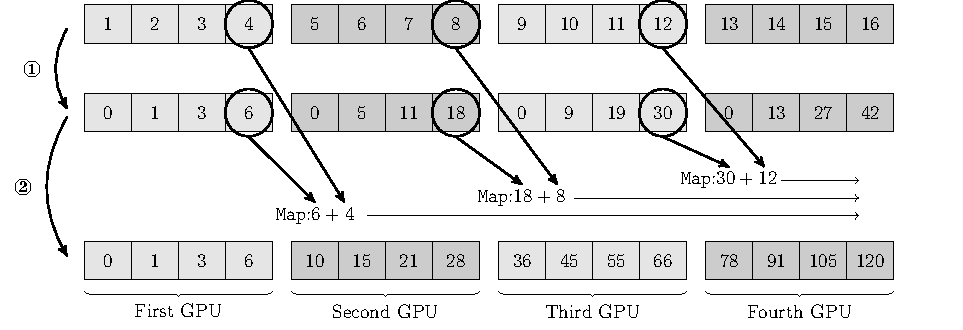
\includegraphics[width=.9\textwidth]{ASHES/scan}
    \caption[Implementation of the \scan skeleton.]%
            {Implementation of the \scan skeleton visualized for four \GPUs:
            (1) All \GPUs scan their parts independently.
            (2) \map skeletons are created automatically and
             executed to produce the result.}
    \label{fig:scan:impl}
\end{figure*}

%The \SkelCL implementation of the \scan skeleton assumes the \GPUs to have a fixed order, such that each \GPU (except the first one) has a predecessor:
%\begin{enumerate}
% \item Every \GPU executes a local scan algorithm for its local part of data;
% \item The results of all \GPUs are downloaded to the \CPU;
% \item For each \GPU (except the first one), a \map skeleton is implicitly created that combines the result of the \GPU's predecessors with all elements of its part using the user-defined operation of the \scan skeleton;
% \item The newly created \map skeletons compute the final results on all \GPUs.
%\end{enumerate}
The output vector is block-distributed among all \GPUs.





\subsubsection{The Stencil Skeleton}
\label{sec:skelcl:stencil}
In stencil applications, the same computation is performed for each element of a container where the computation depends upon neighboring values.
In \autoref{section:skelcl-programming-model} we defined the \stencil skeleton to simplify the development of stencil applications.
The \SkelCL library provides two implementations of the \stencil skeleton.
The first one, called \code{MapOverlap}, supports simple stencil computations;
the second one, called \code{Stencil}, provides support for more complex stencil computations possibly executed iteratively.
In order to achieve high performance, both implementations \code{MapOverlap} and \code{Stencil} use the \GPU's fast local memory.
Both implementations perform the same basic steps on the \GPU:
first, the data is loaded from the global memory into the local memory;
then, the customizing function is called for every data element by passing a pointer to the element's location in the local memory;
finally, the result of the customizing function is copied back into the global memory.
Although both implementations perform the same basic steps, different strategies are implemented for loading the data from the global into the local memory.

In this subsection, we will start by discussing the \code{MapOverlap} implementation and then discuss the \code{Stencil} implementation.
Finally, we will discuss the implementation of the \stencil skeleton for multi-device systems.

\paragraph{The MapOverlap implementation}

We will use the Gaussian blur as an example application to discuss the \code{MapOverlap} implementation.
The Gaussian blur is a standard image processing algorithm used, among other things, for noise reduction.
The color of every pixel of an image is modified by computing a weighted average of the neighboring pixel color values.
The application will be discussed in more detail in \autoref{sec:gauss}.

\autoref{lst:mapoverlap} shows how the \code{MapOverlap} skeleton implementation is used to express the Gaussian blur.
The \code{mapOverlap} function in \autoref{lst:mapoverlap:factory} is customized with a lambda expression which uses its argument, a \code{Neighborhood} object (\autoref{lst:mapoverlap:neighborhood}), to access the neighboring elements with relative indices (\autoref{lst:mapoverlap:indices1} and \autoref{lst:mapoverlap:indices2}).
The second and third argument of the factory function define the range of the stencil shape and the border handling method (\autoref{lst:mapoverlap:borderHandling}).
The actual computation of the Gaussian blur is omitted from \autoref{lst:mapoverlap} for brevity reasons.

\begin{lstlisting}[%
caption={[Implementation of Gaussian blur using the \stencil skeleton.]%
         Implementation of Gaussian blur using the \code{MapOverlap} implementaion of the \stencil skeleton.},%
float={tb},
label={lst:mapoverlap}]
auto gauss = mapOverlap($\label{lst:mapoverlap:factory}$
  [](Neighborhood<char>& in_img) {$\label{lst:mapoverlap:neighborhood}$
      char ul = in_img[{-1, -1}];$\label{lst:mapoverlap:indices1}$
      ...
      char lr = in_img[{+1, +1}];$\label{lst:mapoverlap:indices2}$
      return computeGaussianBlur(ul, ..., lr); },
  1, BorderHandling::NEUTRAL(0));$\label{lst:mapoverlap:borderHandling}$
\end{lstlisting}


\begin{lstlisting}[%
caption={\OpenCL kernel created by the \code{MapOverlap} implementation for the Gaussian blur application.},%
float={tb},
label={lst:mapoverlap:impl}]
#define RANGE (1)   #define NEUTRAL (0)
struct {$\label{lst:mapoverlap:impl:struct:start}$
  local char* data; int row; int col; } char_neighborhood_t;$\label{lst:mapoverlap:impl:struct:end}$

char get(char_neighborhood_t* m, int x, int y) {$\label{lst:mapoverlap:impl:get:start}$
  return m->data[/*computed from RANGE, row, col, x, y*/]; }$\label{lst:mapoverlap:impl:get:end}$

char USER_FUNC(char_neighborhood_t* in_img) {
  char ul = get(in_img, -1, -1);
  ...
  char lr = get(in_img, +1, +1);
  return computeGaussianBlur(ul, ..., lr); }

kernel void mapoverlap(global char* in, global char* out,$\label{lst:mapoverlap:impl:kernel:start}$
          local char* buffer, int numCols, int numRows) {
  ... // load part of in into local buffer$\label{lst:mapoverlap:impl:copy}$
  char_neighborhood_t M;   M.data = buffer;
  M.row = get_local_id(1); M.col = get_local_id(0);
  barrier(CLK_LOCAL_MEM_FENCE);$\label{lst:mapoverlap:impl:barrier}$
  if (/* not out of bound */)
    out[index] = USER_FUNC(&M); }$\label{lst:mapoverlap:impl:call}$
\end{lstlisting}

\autoref{lst:mapoverlap:impl} shows a sketch of the \OpenCL kernel created by the \code{MapOverlap} implementation.
To represent the \code{Neighborhood} object in \OpenCL, a C \code{struct} is created (\autoref{lst:mapoverlap:impl:struct:start}---\autoref{lst:mapoverlap:impl:struct:end}).
A helper function \code{get} (\autoref{lst:mapoverlap:impl:get:start}---\autoref{lst:mapoverlap:impl:get:end}) is created which handles the read access to the data hold by the neighborhood object.
The kernel function \code{mapoverlap}, defined in \autoref{lst:mapoverlap:impl:kernel:start}, first loads the data required by a work-group into a local buffer stored in the fast local \GPU memory (\autoref{lst:mapoverlap:impl:copy}).
It then prepares a neighborhood object and passes it to the customizing function after a boundary check was performed.
A barrier (\autoref{lst:mapoverlap:impl:barrier}) ensures that the loading into the fast local memory has been completed before any work-item executes the customizing function.

Loading of the data into the fast local memory is lengthy and involves performing the boundary checks, therefore, it is not shown in \autoref{lst:mapoverlap:impl}.
%
\begin{figure}
  \begin{centering}
    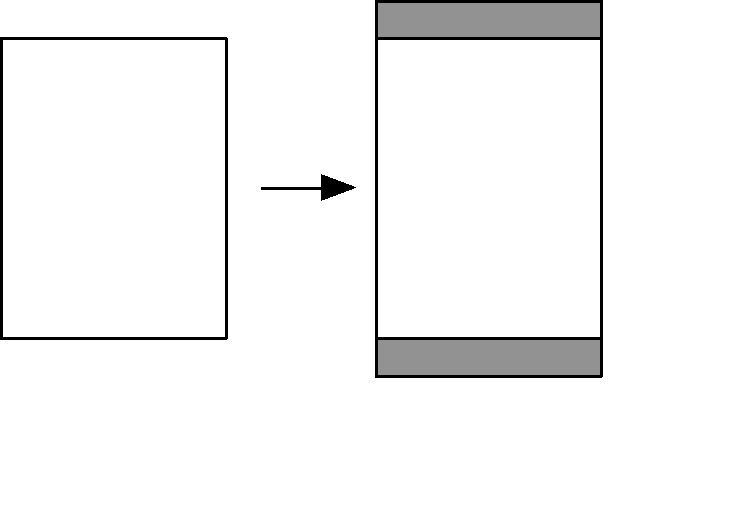
\includegraphics[width=.29\textwidth]{HiStencils/map_overlap}
    \caption[The \code{MapOverlap} implementation of the \stencil skeleton]{The \code{MapOverlap} implementation of the \stencil skeleton prepares a matrix by copying data on the top and bottom}
    \label{fig:mapoverlap:preparation}
    \vspace{-.5em}
  \end{centering}
\end{figure}
%
To minimize the overhead on the \GPU, the \code{MapOverlap} implementation prepares the input matrix on the \CPU before uploading it to the \GPU:
padding elements are appended; they are used to avoid out-of-bounds memory accesses to the top and bottom of the input matrix, as shown in \autoref{fig:mapoverlap:preparation}.
This slightly enlarges the input matrix, but it reduces branching on the \GPU due to avoiding some out-of-bound checks.
In \SkelCL a matrix is stored row-wise in memory on the \CPU and \GPU, therefore, it would be complex and costly to add padding elements on the left and right of the matrix.
To avoid out-of-bound accesses for these regions, the boundary checks are performed on the \GPU.

\paragraph{The Stencil implementation}

We use an iterative stencil application simulating heat flow to discuss the \code{Stencil} implementation.
The application simulates heat spreading from one location and flowing throughout a two-dimensional simulation space.
Let us assume that the heat flows from left to right as indicated by the arrows in \autoref{fig:stencil:first:shape}.
The heat value of a cell is updated based on its (left) neighboring cells.
Multiple iteration steps are required to simulate the flow of heat over a longer distance.

\begin{figure}[t]
  \begin{minipage}[b]{.38\textwidth}
    \centering
    \includegraphics[width=.65\textwidth]{Figures/HiStencils/heat_transfer}
    \caption{Stencil shape for heat simulation}
    \label{fig:stencil:first:shape}
  \end{minipage}
  \hfill %\hspace{.05\textwidth}
  \begin{minipage}[b]{.55\textwidth}
    \begin{lstlisting}[%
      caption={[Heat simulation with the \stencil skeleton]Heat simulation with the \stencil skeleton\vspace{-.9em}},%
      label={lst:stencil:first}]
auto heatSim = skelcl::stencil(
 [](Neighborhood<char>& in) {$\label{lst:stencil:first:func:start}$
  char lt = in[{-1, -1}];
  char lm = in[{-1,  0}];
  char lb = in[{-1, +1}];
  return computeHeat(lt,lm,lb);},$\label{lst:stencil:first:func:end}$
 StencilShape(1, 0, 1, 1),$\label{lst:stencil:first:shape}$
 BorderHandling::NEUTRAL(255));$\label{lst:stencil:first:border}$
heatSim(100_iterations,$\label{lst:stencil:first:iterations}$
        simulationSpace);
    \end{lstlisting}
  \end{minipage}%
\end{figure}

\autoref{lst:stencil:first} shows the implementation of an iterative stencil application simulating heat transfer in \SkelCL.
The application developer specifies the customizing function (\autoref{lst:stencil:first:func:start}---\autoref{lst:stencil:first:func:end}), as well as the extents of the stencil shape (\autoref{lst:stencil:first:shape}) and the out-of-bound handling (\autoref{lst:stencil:first:border}).
The \code{Stencil} implementation allows the stencil shape's extents to be specified using four values for each of the directions:
up, right, down, and left.
In the example in \autoref{lst:stencil:first}, the heat flows from left to right, therefore, no accesses to the elements to the right are necessary and the stencil space's extents are specified accordingly (note the $0$ in \autoref{lst:stencil:first:shape} representing the extent to the right).
\autoref{fig:stencil:first:shape} illustrates this situation: the dark gray element is updated by using the values from the left.
The specified stencil shape's extent is highlighted in light gray.
In our current implementation, the user has to explicitly specify the stencil shape's extents, which is necessary for performing the out-of-bound handling on the \GPU.
In future work, the stencil shape could be inferred from the customizing function using source code analysis in many common cases.
This would help to avoid inconsistencies and free the user from specifying this information explicitly.

Stencil applications often perform stencil computations iteratively, like the heat transfer example which performs multiple iteration steps in order to simulate the transfer of heat over time.
The \code{Stencil} implementation supports iterative execution, which is especially challenging to implement on multi-device systems as we will see later.
On execution of the skeleton, the number of iterations to be performed is specified by the user as the first argument (\autoref{lst:stencil:first:iterations}).
This could be extended in the future, so that the user specifies a function to check if a application specific condition is met and stop the iteration.

The \OpenCL kernel created by the \code{Stencil} implementation looks similar to the \code{MapOverlap} implementation presented in \autoref{lst:mapoverlap:impl}.
The \code{Stencil} implementation uses a slightly different strategy than the \code{MapOverlap} implementation in order to enable the usage of different out-of-bound modes and stencil shapes when using several \stencil skeletons in a sequence, which we discuss in the next paragraph.
To understand why the strategy used by the \code{MapOverlap} implementation is not sufficient for stencil sequences let us consider a situation where two stencil computations are performed one after another and the two stencil shapes used are different.
This cannot be implemented efficiently using \code{MapOverlap}'s implementation strategy, as the input matrix is extended on the \CPU as specified by the first stencil shape.
Therefore, data would have to be downloaded to the \CPU between executions and the data layout would have to be changed.
To avoid this problem, the \code{Stencil} implementation does not append padding elements on the \CPU, but rather manages all out-of-bounds accesses on the \GPU, which slightly increases branching in the code, but enables a more flexible usage of the skeleton.


\paragraph{Sequence of Stencil Operations}
Many real-world applications perform different stencil operations in sequence, like the popular \emph{Canny algorithm}~\cite{NixonAg2012} used for detecting edges in images.
For the sake of simplicity, we consider a version which applies the following steps:
1)~a noise reduction operation is applied, e.\,g., a Gaussian blur;
2)~an edge detection operator like the Sobel filter is applied;
3)~the so-called non-maximum suppression is performed, where all pixels in the image are colored black except pixels being a local maximum;
4)~a threshold operation is applied to produce the final result.
A more complex version of the algorithm performs the edge tracking by hysteresis as an additional step.

Using the \SkelCL library, each single step of the Canny algorithm can be expressed using the \stencil skeleton, as shown in \autoref{lst:stencil:canny}.
The threshold operation performed as the last step, does not need access to, neighboring elements, because the user function only checks the value of a single pixel.
The \code{Stencil} implementation automatically uses the implementation of the simpler (and thus faster) \map skeleton when the user specifies a stencil shape whose extents are $0$ in all directions.
The single steps are combined into a single object of type \code{StencilSequence} which can be executed like a \stencil skeleton.
On execution, it passes its input data to the first stencil defined in the sequence, which passes its output to the next stencil, and so forth.

\begin{lstlisting}[%
  caption={Structure of the Canny algorithm implemented by a sequence of skeletons.},%
  float={tb},
  label={lst:stencil:canny}]
auto gauss     = stencil(...);
auto sobel     = stencil(...);
auto nms       = stencil(...);
auto threshold = stencil(...);

StencilSequence<Pixel(Pixel)>
    canny(gauss, sobel, nms, threshold);
\end{lstlisting}

\paragraph{Targeting Multi-\GPU Systems}
The implicit and automatic support of systems with multiple \OpenCL devices is one of the key features of \SkelCL.
By using distributions, \SkelCL completely liberates the user from error-prone and low-level explicit programming of data (re)distributions on multiple \GPUs.

The \code{MapOverlap} implementation uses the overlap distribution with \textit{border regions} in which the elements calculated by a neighboring device are located.
When it comes to iteratively executing a skeleton, data has to be transferred among devices between iteration steps, in order to ensure that data for the next iteration step is up-to-date.
As the \code{MapOverlap} implementation does not explicitly supports iterations, its implementation is not able to exchange data between devices besides a full down- and upload of the matrix.
% In addition, data exchange has to be performed after each iteration.

The \code{Stencil} implementation explicitly supports iterative execution and, therefore, only exchanges elements from the border region and does not perform a full down- and upload of the matrix, as the \code{MapOverlap} implementation does.
\autoref{fig:syncDevices} shows the \textit{device synchronizations}, \ie, the data exchange performed between two iterations by the \code{Stencil} implementation.
Only the appropriate elements in the \emph{inner border region}, \ie, the border regions adjacent to two \OpenCL devices, are downloaded and stored as \texttt{std::vector}s in a \texttt{std::vector}.
Within the outer vector, the inner vectors are swapped pair-wise on the host, so that the inner border regions can be uploaded in order to replace the out-of-date border regions.

\begin{figure}[tb]
  \centering
  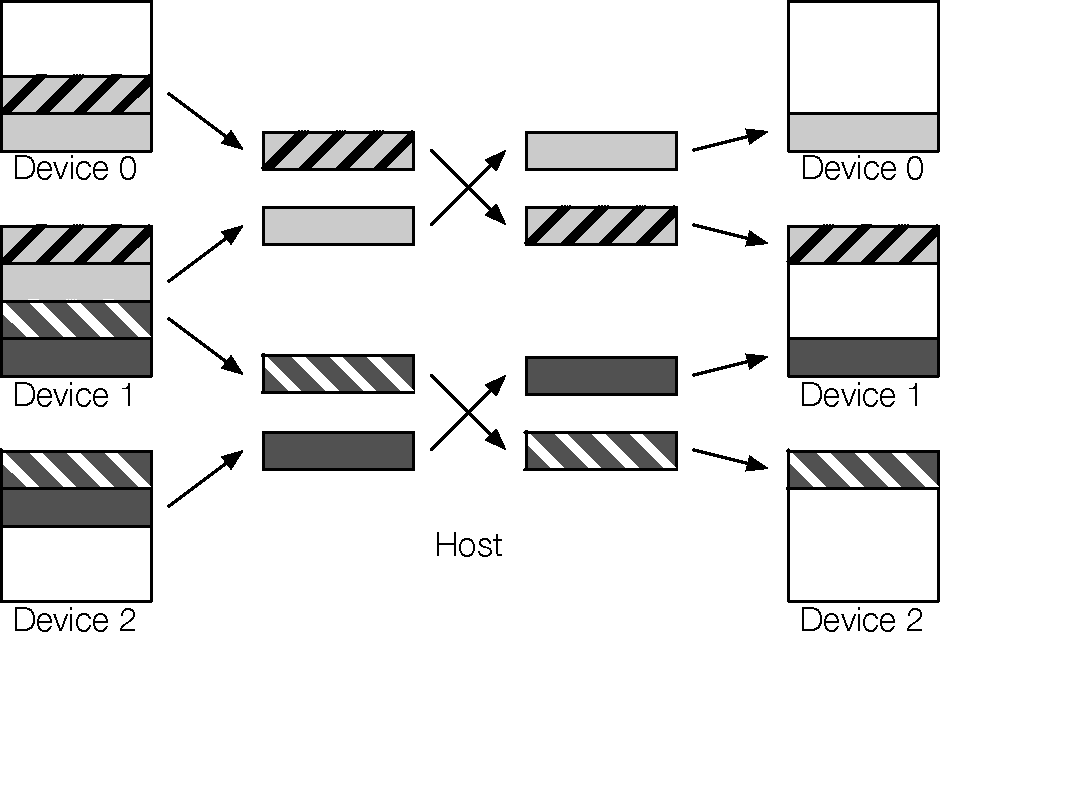
\includegraphics[width=.75\columnwidth]{HiStencils/data_exchange}
  \caption[Device synchronization for three devices during the execution of the \stencil skeleton.]
          {\small Device synchronization for three devices. Equally patterned and colored chunks represent the border regions and their matching inner border region. After the download of the appropriate inner border regions, they are swapped pair-wise on the host. Then the inner border regions are uploaded in order to replace the outdated border regions.}
  \label{fig:syncDevices}
  \vspace{1em}
\end{figure}


By enlarging the number of elements in the border regions, multiple iteration steps can be performed on each device before exchanging data.
However, this introduces redundant computations, such that a trade-off between data exchange and redundant computations has to be found.
For the \code{Stencil} implementation, the user can specify the number of iterations between device synchronizations.
In \cite{Breuer2014} the effects of exploring this parameter space is discussed.
For the investigated applications, the effect of choosing different numbers of iterations between device synchronization was not very large.


\subsubsection{The \allpairs Skeleton}
The \allpairs skeleton defined in \autoref{section:skelcl-programming-model} applies a customizing function to all pairs of vectors from two matrices.
There exist two version of the skeleton: the generic \allpairs skeleton introduced in \autoref{sec:allpairs_skeleton} and the specialized \allpairs skeleton introduced in \autoref{sec:opt_allpairs_skeleton}.
In the specialized version the customizing function is expressed as a composition of the \zip and \reduce skeleton.

In this subsection, we will first discuss the generic and then the specialized implementation.
We will also estimate the performance benefit gained by the specialized implementation.
Finally, we will discuss the implementation of the \allpairs skeleton on multi-device systems.

\paragraph{The Generic Allpairs Skeleton}
\begin{lstlisting}[%
caption={Matrix multiplication expressed using the generic \allpairs skeleton.},%
float=t,%
numbers=left,%
label={lst:allpairs:generic:impl}]
auto mm = allpairs([](const Vector<float>& a,
                      const Vector<float>& b) {
                        float c = 0.0f;
                        for (int i = 0; i < a.size(); ++i)
                          c += a[i] * b[i];
                        return c; });
\end{lstlisting}

\autoref{lst:allpairs:generic:impl} shows the program for computing matrix multiplication using the generic \allpairs skeleton.
The implementation of the customizing function is straightforward.
It is expressed as a lambda expression that receives a pair of vectors, multiplies their elements and sums them up.

\autoref{lst:allpairs:generic:kernel} shows the \OpenCL kernel created after adding and adapting the generic allpairs implementation.
The customizing function (\autoref{lst:allpairs:generic:kernel:funcStart}---\autoref{lst:allpairs:generic:kernel:funcEnd}) has been transformed by the \code{skelclc} compiler.
The vector class has been replaced by an \OpenCL representation (defined in \autoref{lst:allpairs:generic:kernel:structStart} and \autoref{lst:allpairs:generic:kernel:structEnd}) and the element access to the vectors has been replaced by computations of the matching indices.
This implementation assumes that the rows of the first matrix are combined with the columns of the second matrix, as it is required for the matrix multiplication.
% The implementation could easily be extended to support different behavior as well.

The \code{allpairs} kernel function prepares instances of the \code{struct} replacing the vector class in \autoref{lst:allpairs:generic:kernel:prepareStart} and \autoref{lst:allpairs:generic:kernel:prepareEnd}.
After performing a boundary check, the customizing function is called in \autoref{lst:allpairs:generic:kernel:call}.
This \OpenCL kernel is executed once for every element of the output matrix $C$.

\begin{lstlisting}[%
caption={\OpenCL kernel used in the implementation of the generic \allpairs skeleton.},%
float=t,%
numbers=left,%
label={lst:allpairs:generic:kernel}]
struct {$\label{lst:allpairs:generic:kernel:structStart}$
  global float* data; int size; int index; } float_matrix_t;$\label{lst:allpairs:generic:kernel:structEnd}$

float USER_FUNC(float_matrix_t* a, float_matrix_t* b) {$\label{lst:allpairs:generic:kernel:funcStart}$
   float c = 0.0f;
   for (int i = 0; i < a->size; ++i) {
     c +=   a->data[a->index * a->size + i]
          * b->data[i * b->size + b->index]; }
   return c; }$\label{lst:allpairs:generic:kernel:funcEnd}$

kernel void allpairs(const global float* Ap,
                     const global float* Bp,
                           global float* Cp,
                     int n, int d, int m) {
  int col = get_global_id(0); int row = get_global_id(1);
  float_matrix_t A; A.data = Ap; Am.size = d; A.index = row;$\label{lst:allpairs:generic:kernel:prepareStart}$
  float_matrix_t B; B.data = Bp; Bm.size = m; B.index = col;$\label{lst:allpairs:generic:kernel:prepareEnd}$
  if (row < n && col < m)
    Cp[row * m + col] = USER_FUNC(&A, &B); }$\label{lst:allpairs:generic:kernel:call}$
\end{lstlisting}

This generic implementation makes no assumption about the order in which the customizing function (\texttt{USER\_FUNC}) accesses the elements of its two input vectors.
In this generic case, we cannot assume that the two vectors fit entirely into the fast but restricted \GPU local memory.
Therefore, we have to use only the slower global memory in the generic implementation.
On modern \GPUs, accesses to the global memory are very expensive, taking up to 800 processor cycles, as compared to only few cycles required to access the local memory~\cite{CUDAProgrammingGuide}.

Let us assume targeting \GPU architectures and estimate the number of global (and, therefore, expensive) memory accesses required for computing an element of the matrix multiplication in the generic case.
One global memory read access for every element of both input vectors is performed, and a single global memory write access is required to write the result into the output matrix.
Therefore,
\begin{equation}
  n\cdot m\cdot (d + d + 1)
  \label{eq:mm:accesses}
\end{equation}
global memory accesses are performed in total, where $n$ and $m$ are the height and width of matrix $C$ and $d$ is the width of $A$ and the height of $B$.
By using the fast but small local memory, this number of global memory accesses can be reduced and, thus, performance can be improved, as we will see in the next paragraph.
Using the local memory for matrix multiplication is a well-known optimization which we systematically apply to a generic skeleton, rather than to a particular application as usually done in the literature.

\paragraph{The Specialized Allpairs Skeleton}
\autoref{lst:allpairs:special:impl} shows matrix multiplication expressed using the specialized \allpairs skeleton.
\begin{lstlisting}[%
caption={Matrix multiplication expressed using the specialized \allpairs skeleton.},%
float=t,%
numbers=left,%
label={lst:allpairs:special:impl}]
auto mult  = zip([](float x, float y){return x*y;});
auto sumUp = reduce([](float x, float y){return x+y;}, 0);
auto mm    = allpairs(sumUp, mult);
\end{lstlisting}
%
By expressing the customizing function of the \allpairs skeleton as a \zip-\reduce composition, we provide to the skeleton implementation additional semantic information about the memory access pattern of the customizing function, thus allowing for improving the performance.
Our idea of optimization is based on the \OpenCL programming model that organizes \emph{work-items} in \emph{work-groups} which share the same \GPU local memory.
By loading data needed by multiple work-items of the same work-group into the local memory, we can avoid repetitive accesses to the global memory.

\begin{figure}[b]
  \centering
  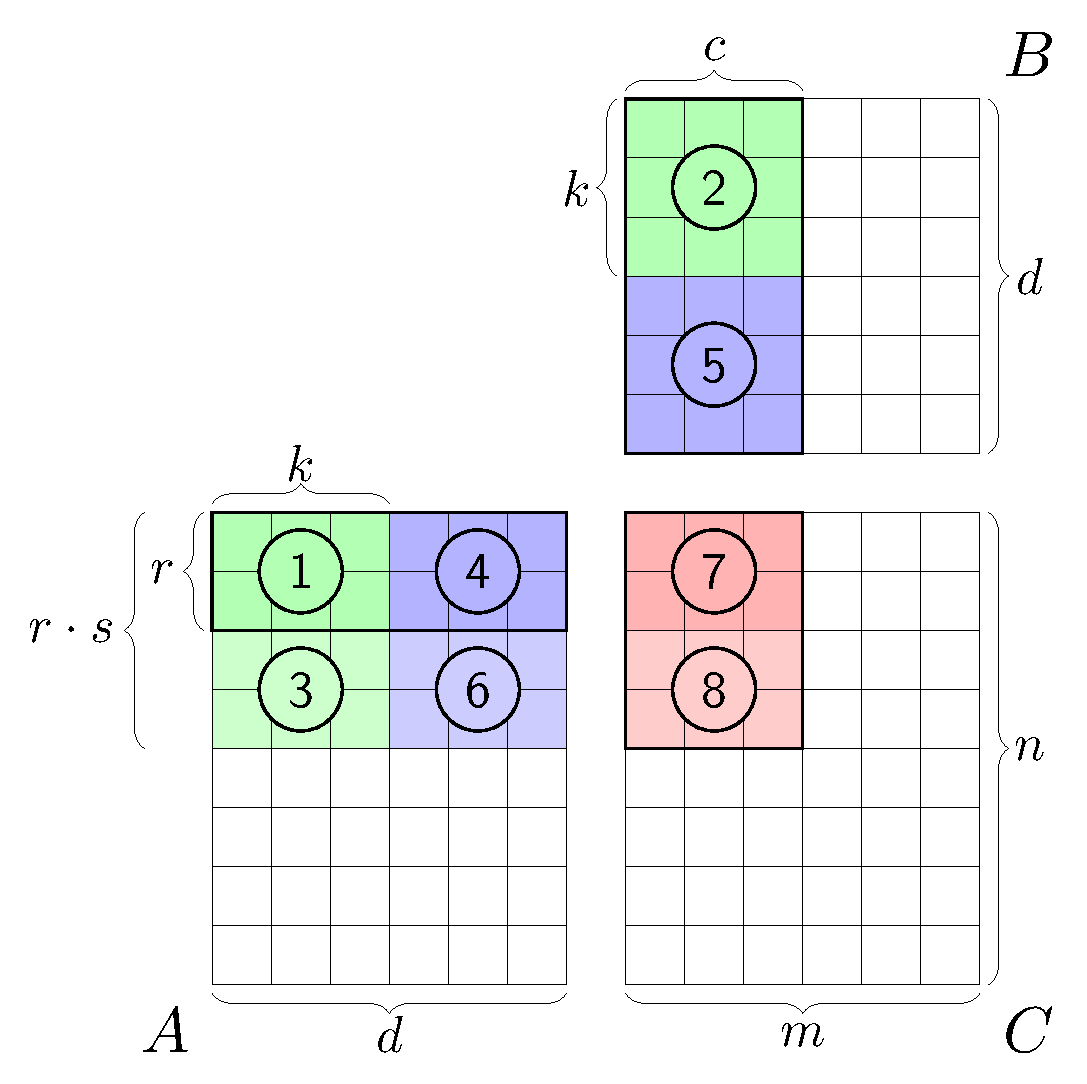
\includegraphics[width=.4\textwidth]{HLPP/memory_access}
  \caption{Implementation schema of the specialized \allpairs skeleton.}
  \label{fig:memory_access}
\end{figure}
For the \allpairs skeleton with the \zip-\reduce customizing function, we can adopt the implementation schema for \GPUs from~\cite{SarjeAl2013}, as shown in \autoref{fig:memory_access}.
We allocate two arrays in the local memory, one of size $r\times k$ ($r=2$, $k=3$ in \autoref{fig:memory_access}) for elements of $A$ and one of size $k\times c$ ($c=3$ in \autoref{fig:memory_access}) for elements of $B$.
A work-group consisting of $c\times r$ work-items computes $s$ blocks ($s=2$ in \autoref{fig:memory_access}) of the result matrix $C$.
In \autoref{fig:memory_access}, the two blocks marked as \circled{7} and \circled{8} are computed by the same work-group as follows.
In the first iteration, the elements of blocks \circled{1} and \circled{2} are loaded into the local memory and combined following the \zip-\reduce pattern.
The obtained intermediate result is stored in block \circled{7}.
Then, the elements of block \circled{3} are loaded and combined with the elements from \circled{2} which still reside in the local memory.
The intermediate result is stored in block \circled{8}.
In the second iteration, the algorithm continues in the same manner with blocks \circled{4}, \circled{5}, and \circled{6}, but this time, the elements of the blocks are also combined with the intermediate results of the first iteration, which are stored in blocks \circled{7} and \circled{8}.
The advantage of computing multiple blocks by the same work-group is that we keep the elements of $B$ in the local memory when computing the intermediate results, \ie, we do not reload block \circled{2} twice for the computation of blocks \circled{7} and \circled{8}.

Every element loaded from the global memory is used by multiple work-items:
\eg, the upper left element of block \circled{1} is loaded only once from the global memory, but used three times:
in the computation of the upper left, upper middle, and upper right elements of \circled{7}.
In general, every element loaded from $A$ is reused $c$ times, and every element from $B$ is reused $r\cdot s$ times.
As the intermediate results are stored in the global memory of matrix $C$, we perform two additional memory accesses (read/write) for every iteration, \ie, $2\cdot \frac{d}{k}$ in total.
Therefore, instead of $n\cdot m\cdot (d + d + 1)$ (see \autoref{eq:mm:accesses}) global memory accesses necessary when using the non-specialized skeleton only
\begin{equation}
  n\cdot m\cdot (\frac{d}{r\cdot s} + \frac{d}{c} + 2\cdot \frac{d}{k})
\end{equation}
global memory accesses are performed.
By increasing the parameters $s$ and $k$, or the number of work-items in a work-group ($c$ and $r$), more global memory accesses can be saved.
However, the work-group size is limited by the \GPU hardware.
While the parameters can be chosen independently of the matrix sizes, we have to consider the amount of available local memory.
\cite{Friese2013}~and~\cite{SarjeAl2013}~discuss how suitable parameters can be found by performing runtime experiments.
In~\cite{Friese2013} the parameters $c = 32$, $r=8$, $s=32$, and $k=64$ are used on modern \GPU hardware showing good performance.

We will report measurements of the performance difference for the two skeleton implementations on real hardware in \autoref{chapter:skelcl-evaluation}.

\paragraph{The Allpairs Skeleton using Multiple GPUs}
\label{sec:allpairs:multi_gpu}
\begin{figure}[b]
  \centering
  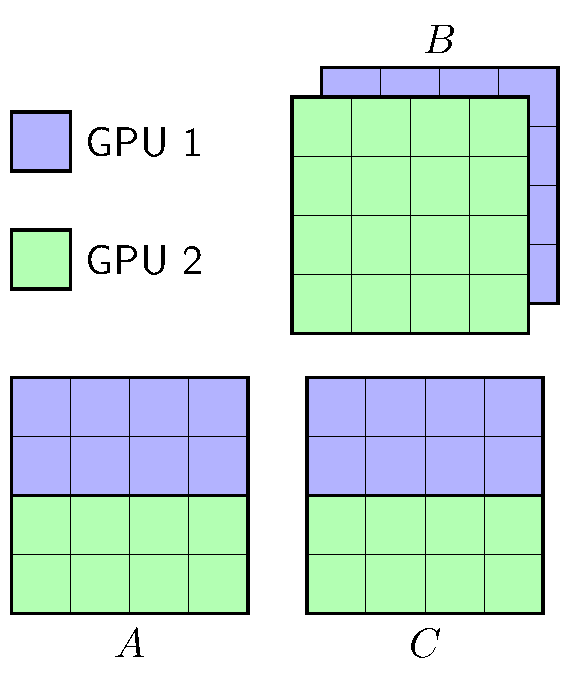
\includegraphics[width=.3\textwidth]{HLPP/multi_gpu}
  \caption[Data distributions used for the \allpairs skeleton for a system with two \GPUs.]%
          {Data distributions used for a system with two \GPUs: matrices $A$ and $C$ are \emph{block} distributed, matrix $B$ is \emph{copy} distributed.}
  \label{fig:multi_gpu}
\end{figure}

The \allpairs skeleton can be efficiently implemented not only on systems with a single \GPU, but on multi-\GPU systems as well.
The necessary data distribution can be easily expressed using two of \SkelCL's \emph{distributions}, as shown in \autoref{fig:multi_gpu}:
Matrix $B$ is \emph{copy} distributed, \ie, it is copied entirely to all \GPUs in the system.
Matrix $A$ and $C$ are \emph{block} distributed, \ie, they are row-divided into as many equally-sized blocks as \GPUs are available;
each block is copied to its corresponding \GPU.
Following these distributions, each \GPU computes one block of the result matrix $C$.
In the example with two \GPUs shown in \autoref{fig:multi_gpu}, the first two rows of $C$ are computed by \GPU 1 and the last two rows by \GPU 2.
The \allpairs skeleton automatically selects these distributions, therefore, the same source code can be used when using a single \GPU or multiple \GPUs.











\subsection{Memory Management Implementation}
\label{section:skelcl-library:memory-management}
In the \SkelCL programming model, the user manages memory using \emph{container data types}.
In the \SkelCL library, the two container data types -- vector and matrix -- are implemented as template classes.
This generic implementation allows for storing data items of any primitive C/\Cpp data type (\eg, \code{int}), as well as user-defined data structures (\code{struct}s).
The implementations follow the \emph{resource acquisition is initialization} (RAII) idiom, which means that they automatically allocate needed resources and free them automatically when the lifetime of the container ends.

\paragraph{The SkelCL Vector}
The \SkelCL vector replicates the interface of the vector from the \Cpp Standard Template Library (\STL), \ie, it can be used as a drop-in replacement of the standard vector.
Internally, a vector comprises pointers to the corresponding areas of main memory (accessible by the host) and device memory.
The vector holds one pointer for the host and one pointer for each device available.
Memory on the devices is allocated automatically, according to the distribution of the vector:
while for a single distributed vector only memory on a single device is allocated, for a vector distributed with the copy, block, or overlap distribution memory on all devices is allocated.
The selected distribution obviously also influences how big the buffers allocated on the devices will be.

Before the execution of a skeleton, the input vector's implementation ensures that all of its data is available on the devices.
This might result in implicit data transfers from the host memory to device memory.
The data of the output vector is not copied back to the host memory but rather resides in the device memory.
Before every data transfer, the vector implementation checks whether the data transfer is necessary;
only then the data is actually transferred.
Hence, if an output vector is used as the input to another skeleton, no further data transfer is performed.
This \emph{lazy copying} in \SkelCL defers data transfers as long as possible or avoids them completely and, thus, minimizes the costly data transfers between host and device.
While all data transfers are performed implicitly by \SkelCL, we understand that experienced application developers may want to have a fine-grained control over the data transfers between host and devices.
For that purpose, \SkelCL offers a set of \APIs which developers can use to explicitly initiate and control the data transfer to and from the devices.

% Implementing such data transfers in \OpenCL manually is a cumbersome task:
% data has to be downloaded to the host before it can be uploaded to other devices, including the corresponding length and offset calculations;
% this results in a lot of low-level code which is completely hidden when using \SkelCL.


\paragraph{The SkelCL Matrix}
The \SkelCL matrix offers an easy to use interface similar to the interface of the vector.
Data is stored in the row-major order and iterators are provided to iterate first over rows and then inside of a single row to access a particular element.
For the copy, block, and overlap distributions, the matrix is divided across rows.
A single row is never split across multiple devices, which simplifies the memory management.
Besides offering an interface to access elements on the host, the matrix also offers an interface for accessing elements on the device by using two-dimensional indices.
This frees the application developer from performing cumbersome index calculations manually.










\subsection{Data Distribution Implementation}
\label{section:skelcl-library:distribution}
The data distributions determine how the data of a container is distributed across multiple devices.
In the \SkelCL library implementation, there exists a class for each data distribution encapsulating the behavior of the distribution.
Every container stores its current data distribution as a member variable.
When the data of the container has to be transferred to or from the devices, the data distribution object is invoked to perform the data transfer operation.

% The data distribution of a container can be changed at runtime either explicitly by the programmer or implicitly by the \SkelCL implementation.
% A change of distribution implies data exchanges between multiple devices and the host, which are performed implicitly by \SkelCL.
% These implicit data exchanges are also performed lazily, \ie, only if really necessary, as described in the previous subsection.

% A special situation arises when the distribution is changed from the \emph{copy} distribution, where each device holds its own full copy of the data.
% In such a case, each device may hold a different version of the container as data modifications are only performed locally on the device.
% In order to maintain \SkelCL's concept of a self-contained container, these different versions must be combined using a user-specified function when the distribution is changed.
% If no function is specified, the copy of the first device is taken as the new version of the container; the copies of the other devices are discarded.


























































% BREAK
\newpage







\from{HIPS begin}
\section{SkelCL: An OpenCL-based skeleton library (HIPS)}

\todo{use in the library section}
SkelCL provides a set of basic skeletons.
Two well-known examples are the \texttt{Zip} skeleton combining two vectors element-wise, and the \texttt{Reduce} skeleton combining all elements of a vector using a binary operation (see Section~\ref{sec:skeletons}).
Listing~\ref{lst:dotproduct} shows how a dot product of two vectors is implemented in SkelCL using these two skeletons.
Here, the \texttt{Zip} skeleton is customized by usual multiplication, and the \texttt{Reduce} skeleton is customized by usual addition.

For comparison, an OpenCL-based implementation of a dot product computation provided by NVIDIA requires approximately 68 lines of code (kernel function: 9~lines, host program: 59~lines)~\cite{CUDASDK-10}.

The implementation principles of the SkelCL library are as follows.
SkelCL generates OpenCL code (\emph{kernel functions}) from skeletons which is then compiled by OpenCL at runtime.
User-defined customizing functions passed to the skeletons are merged with pre-implemented skeleton code during code generation.
Since OpenCL is not able to pass function pointers to GPU functions, user-defined functions are passed as strings in SkelCL.

\begin{lstlisting}[%
breakindent=1.5em,%
caption={SkelCL program computing the dot product of two vectors. Arrays \texttt{a\_ptr} and \texttt{b\_ptr} initialize the vectors.},%
float=tbp,%
label={lst:dotproduct}]
int main (int argc, char const* argv[]) {
    SkelCL::init(); /* initialize SkelCL */

    /* create skeletons */
    SkelCL::Reduce<float> sum (                   "float sum (float x,float y){return x+y;}");
    SkelCL::Zip<float>    mult(                   "float mult(float x,float y){return x*y;}");

    /* allocate and initialize host arrays */
    float *a_ptr = new float[ARRAY_SIZE];
    float *b_ptr = new float[ARRAY_SIZE];
    fillArray(a_ptr, ARRAY_SIZE);
    fillArray(b_ptr, ARRAY_SIZE);

    /* create input vectors */
    SkelCL::Vector<float> A(a_ptr, ARRAY_SIZE);
    SkelCL::Vector<float> B(b_ptr, ARRAY_SIZE);

    /* execute skeletons */
    SkelCL::Scalar<float> C = sum( mult( A, B ) );

    /* fetch result */
    float c = C.getValue();
    
    /* clean up */
    delete[] a_ptr;
    delete[] b_ptr;
}
\end{lstlisting}


\subsubsection{Skeletons in SkelCL}

\todo{use in the library section}
Skeletons are higher-order functions because they take so-called \emph{customizing functions} as parametes.
In SkelCL, skeletons expect the customizing function to be a plain string containing the function's source code.
This is merged with the skeleton's own source code to generate source code for an OpenCL kernel.
After compilation, the kernel function is ready for execution.
Compiling the source code every time from source is a time-consuming task, taking up to several hundreds of milliseconds.
For a small kernel, this can be a huge overhead.
Therefore, SkelCL saves already compiled kernels on disk.
They can be loaded later if the same kernel is used again.
For our applications (presented in Section~\ref{sec:studies}), we observed that loading kernels from disk is at least five times faster than building them from source.

SkelCL currently provides four basic skeletons: \texttt{Map}, \texttt{Zip}, \texttt{Reduce}, and \texttt{Scan}.
Each skeleton consumes vectors as input and produces vectors as output.
A skeleton is called by using the name of the skeleton as a function and passing the appropriate number of arguments to it.
This behavior is implemented using the C++ operator overloading feature.

\subsubsection{Passing Additional Arguments to Skeletons}

\todo{use in the library section}

\begin{lstlisting}[%
caption={Passing additional arguments to a \texttt{Map} skeleton.},%
float=tbp,%
label={lst:additional_args}]
Map<float> mult_num("float f(float input, float number) { return input * number }");

Arguments arguments;
arguments.push(5);

mult_num(input, arguments);
\end{lstlisting}

In general, a skeleton's definition dictates how many input arguments can be passed to the skeleton.
The \texttt{Map} skeleton, for example, specifies that the provided function has to be a unary function, such that only one input vector can be passed to the skeleton.
However, not all algorithms easily fit into this strict pattern.

SkelCL allows the user to pass an arbitrary number of arguments to the function called inside of a skeleton:
first, the function definition must be changed, such that it expects additional arguments;
second, the additional arguments have to be passed to the skeleton upon execution.
A simple example is presented in Listing~\ref{lst:additional_args}.
The function definition for the \texttt{Map} skeleton in the listing takes two arguments instead of one, which would be common for \texttt{Map}.
In this example, an additional increment value is passed to the function.
Thus, the \texttt{Map} skeleton can now be used for adding an arbitrary increment to all elements of an input vector, instead of a fixed increment.
The additional argument is packaged into an \texttt{Arguments} object that is passed to the skeleton.
The implementation ensures passing the argument to all kernel instances called during execution.

Arbitrary types can be passed as arguments; a pointer and the size of the type has to be provided.
It is particularly easy to pass vectors as arguments because no information about the size has to be provided.
The arguments will be passed to the skeleton in the same order in which they are added to the \texttt{Arguments} object.
Hence, their order has to resemble the order of parameters in the function definition.
\from{HIPS end}




\from{ASHES begin}
\section{Overview of SkelCL (ASHES)} 
\subsection{Algorithmic Skeletons}

\todo{use in the library section}
% IMPLEMENTATION
To customize a skeleton, the application developer passes the source code of the user-defined function as a plain string to the skeleton.
SkelCL merges the user-defined function's source code with pre-implemented skeleton-specific program code, thus creating a valid OpenCL kernel automatically.
The created kernel is then compiled by the underlying OpenCL implementation before execution.
Thanks to this procedure SkelCL can operate on top of every standard compliant OpenCL implementation and does not require a customized compiler.

In real-world applications (see, e.\,g., Section~\ref{sec:list-mode_OSEM}), user-defined functions often work not only on a skeleton's input vector, but may also take additional inputs.
With only a fixed number of input arguments, traditional skeletons would not be applicable for the implementation of such applications.
The novelty of SkelCL skeletons is that they can accept additional arguments which are passed to the skeleton's user-defined function.
Since SkelCL's skeletons rely on pre-defined OpenCL code, they are by default not compatible with additional arguments.
Therefore, the SkelCL implementation at runtime adapts this code to the function it uses, such that the skeleton passes its additional arguments to the user-defined function.

% EXAMPLE
Listing~\ref{lst:saxpy} shows an example implementation of the \emph{single-precision real-alpha x plus y} (SAXPY) computation -- a commonly used BLAS routine -- in SkelCL.
\begin{lstlisting}[%
  caption={The BLAS $saxpy$ computation using a zip skeleton with additional arguments},%
float=tbp,%
label={lst:saxpy}]
/* create skeleton Y <- a * X + Y */
Zip<float> saxpy (
    "float func(float x, float y, float a)\
        { return a*x+y; }" );

/* create input vectors */
Vector<float> X(SIZE); fillVector(X);
Vector<float> Y(SIZE); fillVector(Y);
float a = fillScalar();

Y = saxpy( X, Y, a );      /* execute skeleton */

print(Y.begin(), Y.end()); /* print results */
\end{lstlisting}
SAXPY is a combination of scalar multiplication of $a$ with vector $X$ followed by vector addition with $Y$.
In the example, the computation is implemented by a zip skeleton:
vectors $X$ and $Y$ are passed as input, while factor $a$ is passed to the user-defined function as an additional argument.
The additional argument is simply appended to the argument list when the skeleton is executed.
Note that all input values of the user-defined function are scalar values rather than vectors or pointers.
Besides scalar values, like shown in the example, vectors can also be passed as additional arguments to a skeleton.
This feature is implemented in SkelCL using variadic templates from the new C++ standard\cite{gregor08, c++11}.

\section{Programming Multi-GPU Systems (ASHES)}

Additional challenges arise when a system comprises multiple GPUs.
In particular, communication and coordination between multiple GPUs and the host have to be implemented.
Many low-level details, like pointer arithmetics and offset calculations, are necessary when using OpenCL or CUDA for this purpose.
In this section, we demonstrate how SkelCL helps the developer to program multi-GPU systems at a high level of abstraction.

% \subsection{Data distribution}

% SkelCL's vector data type abstracts from memory ranges on multiple GPUs, such that the vector's data is accessible by each GPU.
% However, each GPU may access different parts of a vector or may even not access it at all.
% For example, when implementing work-sharing on multiple GPUs, the GPUs will access disjoint parts of input data, such that copying only a part of the vector to a GPU would be more efficient than copying the whole data to each GPU.

% For specifying partitionings of vectors in multi-GPU systems, the concept of \emph{distribution} is introduced in SkelCL.
% A distribution describes how the vector's data is distributed among the available GPUs.
% It allows the programmer to abstract from the challenges of managing memory ranges which are shared or partitioned across multiple devices: the programmer can think of a distributed vector as of a self-contained entity.

% Figure~\ref{fig:distributions} shows three distributions which are currently implemented in SkelCL and offered to the programmer:
% \emph{single}, \emph{block}, and \emph{copy}.
% If set to \emph{single} distribution (Figure~\ref{fig:distributions:single}), vector's whole data is stored on a single GPU (the first GPU if not specified otherwise).
% With \emph{block} distribution (Figure~\ref{fig:distributions:block}), each GPU stores a contiguous, disjoint part of the vector.
% The \emph{copy} distribution (Figure~\ref{fig:distributions:copy}) copies vector's entire data to each available device.
% A newly created vector can adopt any of these distributions.

% \begin{figure}[tb]
%   \centering
%   \begin{subfigure}{.30\textwidth}
%     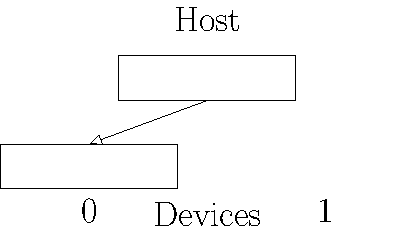
\includegraphics[width=\textwidth]{ASHES/singleDistribution}
%     \caption{\emph{single}}
%     \label{fig:distributions:single}
%   \end{subfigure}
%   \hfill
%   \begin{subfigure}{.30\textwidth}
%     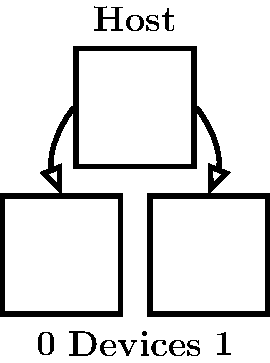
\includegraphics[width=\textwidth]{ASHES/copyDistribution}
%     \caption{\emph{copy}}
%     \label{fig:distributions:copy}
%   \end{subfigure}
%   \hfill
%   \begin{subfigure}{.30\textwidth}
%     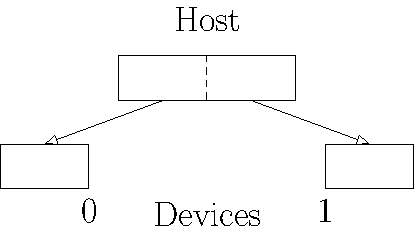
\includegraphics[width=\textwidth]{ASHES/blockDistribution}
%     \caption{\emph{block}}
%     \label{fig:distributions:block}
%   \end{subfigure}
%   \caption{Distributions of a vector in SkelCL.}
%   \label{fig:distributions}
%   \bigskip
% \end{figure}

% The vector distribution can be changed at runtime either explicitly by the programmer or implicitly by the system.
% A change of distribution implies data exchanges between multiple GPUs and the host, which are performed implicitly by SkelCL.
% These implicit data exchanges are also performed lazily, i.\,e. only if really necessary, as described in Section~\ref{sec:introduction_to_skelcl}.
% Implementing such data transfers in OpenCL manually is a cumbersome task:
% data has to be downloaded to the host before it can be uploaded to other devices, including the corresponding length and offset calculations;
% this results in a lot of low-level code which is completely hidden when using SkelCL.

% A special situation arises when the distribution is changed from the \emph{copy} distribution, where each GPU holds its own full copy of the data.
% In such a case, each GPU may hold a different version of the vector as data modifications are only performed locally on the GPU.
% In order to maintain SkelCL's concept of a self-contained vector, these different versions must be combined using a user-specified function when the distribution is changed.
% If no function is specified, the copy of the first device is taken as the new version of the vector; the copies of the other devices are discarded.

\subsection{Skeletons for Multiple GPUs}
\label{sec:multi-gpu_skeletons}

The skeletons of SkelCL possess specific features for working in multi-GPU systems.
They take into account the distribution of their input vectors: each GPU that holds a part or a complete copy of a vector is involved in the execution of the skeleton.
Therefore, all GPUs automatically cooperate in the skeleton execution if its input vector is \emph{block}-distributed, whereas the skeleton is executed on one GPU if the vector distribution is \emph{single}.
If a skeleton's input vector is \emph{copy}-distributed, then all GPUs execute the same skeleton on their own copies.

Vectors can be passed to skeletons either as main inputs or as additional arguments.
For main input vectors, a skeleton-specific default distribution is set automatically by SkelCL, but the programmer can override the defaults, i.\,e., specify a distribution that fits best for the application.
For vectors passed as an additional argument, no meaningful default distribution can be provided by the system, because the access pattern for the vector is determined by the user-defined function.
Therefore, the user has to specify explicitly the distribution for these vectors.

\subsection{Implementation of Skeletons on Multiple GPUs}

\paragraph{Map and zip}
In a multi-GPU setting, each GPU executes the map's unary function on its part of the input vector.
The same holds for the zip skeleton, but it requires both input vectors to have the same distribution, and, in case of the single-distributed vectors, they also have to be stored on the same GPU.
If this requirement is not satisfied, SkelCL automatically changes the input vector distribution to block distribution.
This distribution is also set by default for input vectors with no distribution specified by the user.
Both, the map and zip skeleton, set their output vector distribution to that of their input vectors.

\paragraph{Reduce}
The reduce skeleton automatically performs all necessary synchronization and communication between CPU and GPUs, in three steps:
\begin{enumerate}
 \item Every GPU executes a local reduction for its local part of data;
 \item The results of all GPUs are gathered by the CPU;
 \item The CPU reduces these intermediate results to compute the final result.
\end{enumerate}
The output vector of the reduce skeleton holds only a single element, therefore, the output vector distribution is set to single.

\paragraph{Scan}
An example of the scan skeleton executed on four devices using addition as operation is shown in Figure~\ref{fig:scan}.
The input vector $[1,\ldots,16]$ is distributed using the \emph{block} distribution by default (shown in the top line).
After performing the scan algorithm on all devices (second line of the figure), map skeletons are built implicitly using the marked values and executed on all devices except the first one.
This produces the final result, as shown in the bottom line.

\begin{figure*}[tbp]
    \centering
    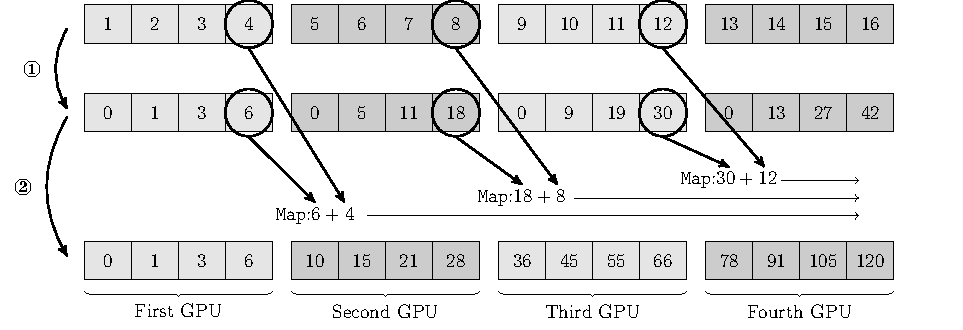
\includegraphics[width=.9\textwidth]{ASHES/scan}
    \caption{Scan on four GPUs: (1) All GPUs scan their parts independently.
            (2) map skeletons are created automatically and
             executed to produce the result.}
    \label{fig:scan}
\end{figure*}

The SkelCL implementation of the scan skeleton assumes the GPUs to have a fixed order, such that each GPU (except the first one) has a predecessor:
\begin{enumerate}
 \item Every GPU executes a local scan algorithm for its local part of data;
 \item The results of all GPUs are downloaded to the host;
 \item For each GPU (except the first one), a map skeleton is implicitly created that combines the result of the GPU's predecessors with all elements of its part using the user-defined operation of the scan skeleton;
 \item The newly created map skeletons compute the final results on all GPUs.
\end{enumerate}
The output vector is block-distributed among all GPUs.
\from{ASHES end}




\from{Paraphrase begin}
\section{SkelCL (Paraphrase)}

\subsection{The MapOverlap Skeleton}
Many applications dealing with two-dimensional data perform calculations for every data element taking neighboring data elements into account.
For example, image processing algorithms, like the gaussian blur, calculate a new value for every pixel of an input image using the previous value of the pixel and its surrounding values.

To facilitate the development of such applications, we extend SkelCL by an additional skeleton in combination with a new matrix data type, which is presented in Section~\ref{sec:skelcl:matrix}.
This skeleton can be used with either vector or matrix data type.
We explain the details of the new skeleton for the matrix data type.
\begin{itemize}
  \item The \emph{MapOverlap} skeleton takes two parameters: a function $f$ and an integer value $d$.
   It applies $f$ to each element of an input matrix $m_{in}$ while taking the neighboring elements within the range $[-d, +d]$ in each dimension into account, i.\,e.
  \begin{align*}
m_{out}[i,j]=f\left(
\begin{array}{ccccc}
m_{in}[i-d,j-d] & \hdots & m_{in}[i-d,j] & \hdots & m_{in}[i-d,j+d] \\
\vdots & ~ & \vdots & ~ & \vdots \\
m_{in}[i,j-d] & \hdots & m_{in}[i,j] & \hdots & m_{in}[i,j+d]\\
\vdots & ~ & \vdots & ~ & \vdots \\
m_{in}[i+d,j-d] & \hdots & m_{in}[i+d,j] & \hdots & m_{in}[i+d,j+d] \\
\end{array}
\right)
\end{align*}
\end{itemize}

In the actual source code, the application developer provides the function $f$ which receives a pointer to the element in the middle, $m_{in}[i,j]$.
Listing~\ref{lst:mapoverlap01} shows a simple example of computing the sum of all direct neighboring values using the MapOverlap skeleton.
To access the elements of the input matrix $m_{in}$, function \texttt{get} is used, as provided by SkelCL.
All indices are specified relative to the middle element $m_{in}[i,j]$, therefore, for accessing this element the function call \texttt{get(m\_in, 0, 0)} is used.

The application developer must ensure that only elements in the range specified by the second argument $d$ of the MapOverlap skeleton, are accessed.
In Listing~\ref{lst:mapoverlap01}, range is specified as $d=1$, therefore, only direct neighboring elements are accessed.
To enforce this property, boundary checks are performed at runtime by the \texttt{get} function.
In future work, we plan to avoid boundary checks at runtime by statically proving that all memory accesses are in bounds, as it is the case in the shown example.

Special handling is necessary when accessing elements out of the boundaries of the matrix, e.g., when the item in the top-left corner of the matrix accesses elements above and left of it.
The MapOverlap skeleton can be configured to handle such out-of-bound memory accesses in two possible ways:
1) a specified neutral value is returned;
2) the nearest valid value inside the matrix is returned.
In Listing~\ref{lst:mapoverlap01}, the first option is chosen and $0.0$ is provided as neutral value.

\begin{lstlisting}[%
caption={MapOverlap skeleton computing the sum of all direct neightbors for every element in a matrix},%
float=tbp,%
label={lst:mapoverlap01}]
MapOverlap<float(float)> m("float func(float* m_in){
     float sum = 0.0f;
     for (int i = -1; i < 1; ++i)
       for (int j = -1; j < 1; ++i)
         sum += get(m_in, i, j);
     return sum;
   }", 1, SCL_NEUTRAL, 0.0f);
\end{lstlisting}

Listing~\ref{lst:raw_opencl01} shows how the same simple calculation can be performed in standard OpenCL.
While the amount of lines of code increases by a factor of 2, the complexity of each single line also increases, as follows.
Besides a pointer to the output memory, the width of the matrix has to be provided as parameter.
The correct index has to be calculated for every memory access using an offset and the width of the matrix.
Therefore, knowledge about how the two-dimensional matrix is stored in one-dimensional memory is required.
In addition, manual boundary checks have to be performed to avoid faulty memory accesses.\bigskip

\begin{lstlisting}[%
caption={An OpenCL kernel performing the same calculation as the MapOverlap skeleton shown in Listing~\ref{lst:mapoverlap01}.\bigskip},%
label={lst:raw_opencl01}]
__kernel void sum_up(__global float* m_in,
                     __global float* m_out,
                     int width, int height) {
  int i_off = get_global_id(0); int j_off = get_global_id(1);
  float sum = 0.0f;
  for (int i = i_off - 1; i < i_off + 1; ++i)
    for (int j = j_off - 1; j < j_off + 1; ++j) {
      // perform boundary checks
      if ( i < 0 || i > width || j < 0 || j > height )
        continue;
      sum += m_in[ j * width + i ];     }
  m_out[ j_off * width + i_off ] = sum; }
\end{lstlisting}

SkelCL avoids all these low-level details.
Neither additional parameter, nor index calculations or manual boundary checks are necessary.
In SkelCL, the application developer only provides the source code implementing the steps required by the algorithm.

\subsection{Data distribution on multiple devices}
\label{sec:data_distribution}
The key feature of SkelCL for multi-device systems is that SkelCL's data types abstract from memory ranges on multiple devices, i.\,e. the data is accessible by each device.
However, each device may access different parts of a container (vector or matrix) or may even not access it at all.
For example, when implementing work-sharing on multiple devices, the devices will usually access disjoint parts of input data, such that copying only a part of the container to a device would be more efficient than copying the whole data to each device.

To simplify the specification of partitionings of containers in programs for multi-device systems, SkelCL implements the \emph{distribution} mechanism that describes how a container is distributed among the available devices.
It allows the programmer to abstract from managing memory ranges which are shared or spread across multiple devices:
the programmer can think of a distributed container as of a self-contained entity.

Four kinds of distribution are currently implemented in SkelCL and offered to the programmer:
\emph{block}, \emph{copy}, \emph{single} and \emph{overlap} (see Figure~\ref{fig:distributions}).
With \emph{block} distribution (Figure~\ref{fig:distributions:block}), each device stores a contiguous, disjoint part of the container.
The \emph{copy} distribution (Figure~\ref{fig:distributions:copy}) copies container's entire data to each available device.
In case of \emph{single} distribution (Figure~\ref{fig:distributions:single}), container's whole data is stored on a single device (the first device by default).

Together with the matrix data type, we introduce a new distribution called \emph{overlap} (Figure~\ref{fig:distribution:overlap}).
The overlap distribution splits the matrix into one chunk for each device, similarly to the block distribution.
In addition to the block distribution, the following holds for an overlap-distributed matrix:
each chunk consists of a number of continuous rows, and, a parameter -- the \emph{overlap size} -- specifies the number of rows at the edges of a chunk which are copied to the two neighboring devices.
Figure~\ref{fig:distribution:overlap} illustrates the overlap distribution:
Device 0 receives the top chunk ranging from the top row to the middle, while device 1 receives the second chunk ranging from the middle row to the bottom.
The marked regions are the \emph{overlap regions} which are available on both devices.

The \emph{overlap} distribution is automatically selected as distribution by the MapOverlap skeleton, to ensure that every device has access to the neighboring elements as needed by the MapOverlap skeleton.

A programmer can set the distribution of containers explicitly, or every skeleton selects a default distribution for its input and output containers otherwise.
Container's distribution can be changed at runtime.
A change of distribution implies data exchanges between multiple devices and the host, which are performed by SkelCL implicitly and lazily, as described above.
Implementing such data transfers in the standard OpenCL is a cumbersome task:
data has to be downloaded to the host before it can be uploaded to other devices, including the corresponding length and offset calculations;
this results in a lot of low-level code which is completely hidden when using SkelCL.
\from{Paraphrase end}



\from{HLPP begin}
\section{The Allpairs Skeleton and its Implementation (HLPP)}
\label{sec:allpairs_skeleton}

\label{sec:formal_def}
We define the allpairs computation pattern for two sets of entities, each entity represented by a vector of length $d$.
Let the cardinality of the first set be $n$ and the cardinality of the second set be $m$.
We model the first set as a $n\times d$ matrix $A$ and the second set as a $m\times d$ matrix $B$.
The allpairs computation yields an output matrix $C$ of size $n\times m$ as follows:
$c_{i, j} = A_i \oplus B_j$, where $A_i$ and $B_j$ are row vectors of $A$ and $B$, correspondingly:
$A_i = [A_{i,1}, \cdots, A_{i, d}]$, $B_j = [B_{j,1}, \cdots, B_{j,d}]$, and $\oplus$ is a binary operator defined as vectors.

\begin{definition}
  \label{def:allpairs}
  Let $A$ be a $n\times d$ matrix, $B$ be a $m\times d$ matrix, and $C$ be a $n\times m$ matrix, with their elements $a_{i,j}$, $b_{i,j}$, and $c_{i,j}$ respectively.
  The algorithmic skeleton \emph{allpairs} with customizing binary function $\oplus$ is defined as follows:
  \[
    \allpairs(\oplus)\left(
      \left[ \begin{array}{ccc}%
 	      a_{1,1} & \cdots & a_{1,d}\\[.25em]
       	\vdots & & \vdots\\[.25em]
       	a_{n,1} & \cdots & a_{n,d}%
     	\end{array}\right],%
      \left[ \begin{array}{ccc}%
       	b_{1,1} & \cdots & b_{1,d}\\[-.25em]
       	\cdot & & \cdot\\[-.75em]
       	\cdot & & \cdot\\[-.25em]
       	b_{m,1} & \cdots & b_{m,d}%
   	\end{array}\right]\right)%
  	\eqdef 
      \left[ \begin{array}{ccc}%
 	      c_{1,1} & \cdots & c_{1,m}\\[.25em]
       	\vdots & & \vdots\\[.25em]
        c_{n,1} & \cdots & c_{n,m}%
   	\end{array}\right]
  \]
  where elements $c_{i,j}$ of the $n\times m$ matrix $C$ are calculated as follows:
  \[
	  c_{i,j} = \DottedVector{a_{i,1}}{a_{i,d}} \oplus \DottedVector{b_{j,1}}{b_{j,d}}
  \]
\end{definition}

Figure~\ref{fig:allpairs_access_a} illustrates this definition:
the element $c_{2,3}$ of matrix $C$ marked as \circled{3} is computed by combining the second row of $A$ marked as \circled{1} with the third row of $B$ marked as \circled{2} using the binary operator $\oplus$.
Figure~\ref{fig:allpairs_access_b} shows the same computation with the transposed matrix $B$.
\begin{figure}[b]
  \centering
	\includegraphics[width=0.44\textwidth]{HLPP/allpairs_access_pattern_alternative}
	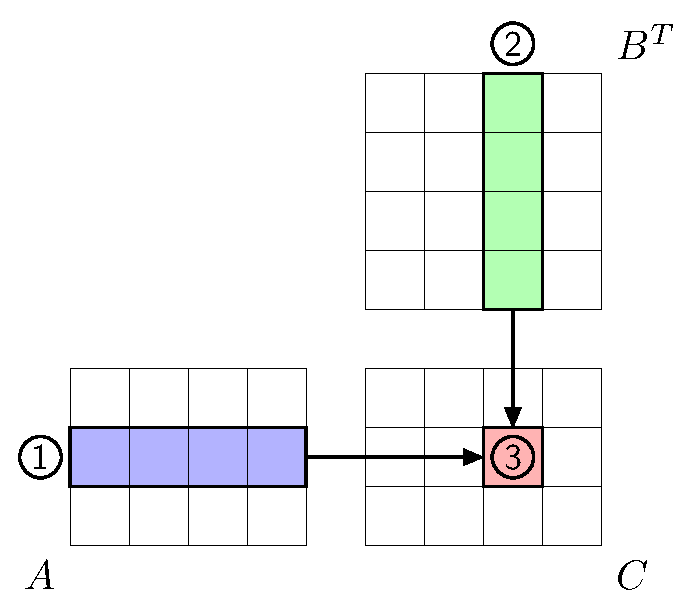
\includegraphics[width=0.44\textwidth]{HLPP/allpairs_access_pattern}
  \caption{The allpairs computation. Left: element $c_{2,3}$
    (\protect\tikz[baseline=(char.base)]\protect\node[shape=circle,draw,inner sep=1pt] (char) {3};)
    is computed by combining the second row of $A$
    (\protect\tikz[baseline=(char.base)]\protect\node[shape=circle,draw,inner sep=1pt] (char) {1};)
    with the third row of $B$
    (\protect\tikz[baseline=(char.base)]\protect\node[shape=circle,draw,inner sep=1pt] (char) {2};)
    using the binary operator $\oplus$. Right: the transposed matrix $B$ is used.}
  \label{fig:allpairs_access}
\end{figure}

\vspace{6em}
Let us consider two example applications which can be expressed by customizing the allpairs skeleton with a particular function $\oplus$.

\paragraph{Example 1:}
The Manhattan distance (or $L_1$ distance) is a measure of distance which is used in many applications.
In general, it is defined for two vectors, $v$ and $w$, of equal length $d$, as follows:
\begin{equation}
  \label{eq:man_dist}
  \ManDist(v, w) = \sum_{k=1}^d | v_k - w_k | 
\end{equation}
In~\cite{DaDQR-09}, the so-called Pairwise Manhattan Distance (\emph{PMD}) is studied as a fundamental operation in hierarchical clustering for data analysis.
\emph{PMD} is obtained by computing the Manhattan distance for every pair of rows of a given matrix.
This computation for arbitrary matrix $A$ can be expressed using the allpairs skeleton customized with the Manhattan distance defined in (\ref{eq:man_dist}):
\begin{equation}
  \PMD(A) = \mbox{\emph{allpairs}}(\mbox{\emph{ManDist}})\left(A, A\right)
\end{equation}
The $n\times n$ matrix computed by the customized skeleton contains the Manhattan distance for every pair of rows of the input $n\times d$ matrix $A$.

\paragraph{Example 2:}
Matrix multiplication is a basic linear algebra operation, which is a building block of many scientific applications.
An $n\times d$ matrix $A$ is multiplied by a $d\times m$ matrix $B$, producing a $n\times m$ matrix $C=A\times B$ whose element $c_{i,j}$ is computed as the dot product of the $i$th row of $A$ with the $j$th column of $B$.
The dot product of two vectors $a$ and $b$ of length $d$ is computed as:
\begin{equation}
  \dotProduct (a,b) = \sum_{k=1}^d a_k \cdot b_k
\end{equation}
The matrix multiplication can be expressed using the allpairs skeleton as:
\begin{equation}
  A\times B = \allpairs(\dotProduct)\left(A, B^T\right)
  \label{eq:mat_mult_allpairs}
\end{equation}
where $B^T$ is the transpose of matrix $B$.
We will use the matrix multiplication as our running example for the allpairs skeleton throughout the paper.

\vspace{1em}
We develop the allpairs skeleton within the skeleton library SkelCL~\cite{StKG-12}, which is built on top of OpenCL and targets modern parallel systems with multiple GPUs.
Currently, five other skeletons are available in SkelCL: \emph{map}, \emph{zip}, \emph{reduce}, \emph{scan}, and \emph{mapOverlap}.
Skeletons operate on container data types (in particular vectors and matrices) which alleviate the memory management of GPUs:
data is copied automatically to and from GPUs, instead of manually performing data transfers as required in OpenCL.
For programming multi-GPU systems, SkelCL offers the application programmer a data distribution mechanism to specify how the data of a container is distributed among the GPUs in the system.
The container's data can either be assigned to a single GPU, be copied to all GPUs, or be partitioned in equal blocks across the GPUs, possibly with an overlap.
If the data distribution is changed in the program, the necessary data movements are done automatically by the system~\cite{StKG-12}.

\begin{lstlisting}[%                                                             
caption={Matrix multiplication in SkelCL using the \emph{allpairs} skeleton.},%
float=t,%                                                                       
numbers=left,%
label={lst:basic_mm}]
skelcl::init();
Allpairs<float(float, float)> mm(
 "float func(float_matrix_t a, float_matrix_t b) {\
  float c = 0.0f;\
  for (int i = 0; i < width(a); ++i) {\
    c += getElementFromRow(a, i) * getElementFromCol(b, i); }\
  return c; }");
Matrix<float> A(n, k); fill(A);
Matrix<float> B(k, m); fill(B);
Matrix<float> C = mm(A, B);
\end{lstlisting}

Listing~\ref{lst:basic_mm} shows the SkelCL program for computing matrix multiplication using the \emph{allpairs} skeleton;
the code follows directly from the mathematical formulation (\ref{eq:mat_mult_allpairs}).
In the first line, the SkelCL library is initialized.
Skeletons are implemented as classes in SkelCL and customized by instantiating a new object, like in line 2.
The \texttt{Allpairs} class is implemented as a template class specified with the data types of matrices involved in the computation (\texttt{float(float, float)}).
This way the implementation can ensure the type correctness by checking the types of the arguments when the skeleton is executed in line 10.
The customizing function -- specified as a string (line 3 -- 7) -- is passed to the constructor.
Data types for matrices (\texttt{float\_matrix\_t} in line 3) are defined by the SkelCL implementation and used as arguments of helper functions for accessing elements from both matrices (line 6).
The transpose of matrix $B$ required by the definition (\ref{eq:mat_mult_allpairs}) is implicitly performed by accessing elements from the columns of $B$ using the helper function \texttt{getElementFromCol}.
After initializing the two input matrices (line 8 and 9), the calculation is performed in line 10.

In our SkelCL library, skeletons are implemented by translating them into executable OpenCL code.
Listing~\ref{lst:basic_impl} shows the OpenCL kernel which is combined with the given customizing function by the implementation of the allpairs skeleton.
The customizing function (named \texttt{\emph{func}} in Listing~\ref{lst:basic_mm}) is renamed to match the name used in the function call in the implementation (\texttt{USER\_FUNC} in Listing~\ref{lst:basic_impl}).
In addition, the types used in the predefined OpenCL kernel (\texttt{TYPE\_LEFT}, \texttt{TYPE\_RIGHT}, and \texttt{TYPE\_OUT} in Listing~\ref{lst:basic_impl}) are adjusted to match the actual types of the elements used in the computation (in this case, all three types are \texttt{float}).
These modifications ensure that a valid OpenCL program performing the allpairs calculation is constructed.
This generated OpenCL program is executed once for every element of the output matrix $C$.
In lines 6 -- 7, the implementation prepares variables (\texttt{Am} and \texttt{Bm}) of a predefined data type (\texttt{float\_matrix\_t}) which encapsulate the matrices $A$ and $B$ and passes them to the customizing function which is called in line 9.

\begin{lstlisting}[%                                                             
caption={Generic OpenCL kernel used in the implementation of the allpairs skeleton.},%
float=t,%                                                                       
numbers=left,%
label={lst:basic_impl}]
__kernel void allpairs(const __global TYPE_LEFT*  A,
                       const __global TYPE_RIGHT* B,
                             __global TYPE_OUT*   C,
                             int n, int d, int m) {
  int col = get_global_id(0); int row = get_global_id(1);
  float_matrix_t Am; Am.data = A; Am.width = d; Am.row = row;
  float_matrix_t Bm; Bm.data = B; Bm.width = m; Bm.col = col;
  if (row < n && col < m)
    C[row * m + col] = USER_FUNC(Am, Bm); }
\end{lstlisting}

To achieve high performance, skeleton implementations must efficiently exploit the complex memory hierarchy of multi-GPU architectures.
There are two main types of memory in OpenCL: \emph{global} and \emph{local memory}.
The global memory is typically large but slow; the local memory is small but fast and has similar performance as caches in traditional systems, but has to be programmed manually.
On modern GPUs, accesses to the global memory are very expensive, taking up to 800 processor cycles, as compared to only few cycles required to access the local memory~\cite{NVIDIA-12}.

The generic implementation of the allpairs skeleton in Listing~\ref{lst:basic_impl} makes no assumption about the order in which the customizing function (\texttt{USER\_FUNC}) accesses the elements of its two input vectors.
In this general case, we cannot assume that the two vectors fit entirely into the restricted GPU local memory.
Therefore, we have to use only the global memory in the generic implementation.
To improve our implementation of the allpairs skeleton, we restrict the memory access pattern of the customizing function in the next section.


\section{The Specialized Allpairs Skeleton (HLPP)}
\label{sec:opt_allpairs_skeleton}
In this section, we first analyze the memory access pattern of the matrix multiplication and then observe that this pattern can also be found in some other allpairs computations.
We, therefore, define a specialized version of the allpairs skeleton, which is suitable for applications having this pattern, and show how it can be implemented more efficiently than the generic skeleton.

\subsection{The memory access pattern of the matrix multiplication}
Figure~\ref{fig:single_memory_access} shows the memory access pattern of the matrix multiplication for $4\times 4$ matrices.
\begin{figure}[t]
  \centering
  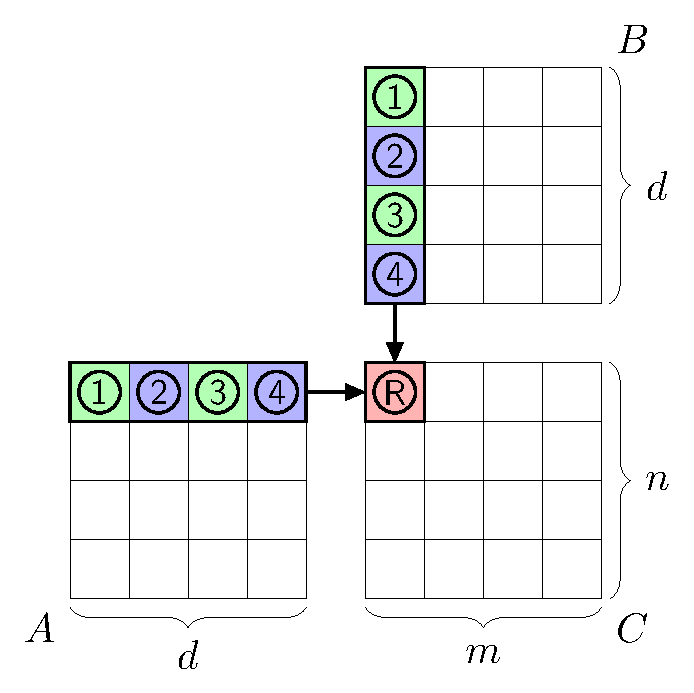
\includegraphics[width=0.4\textwidth]{HLPP/single_memory_access}
  \caption{Memory access pattern of the matrix multiplication $A\times B = C$.}
  \label{fig:single_memory_access}
\end{figure}
To compute the element \circled{R} of the result matrix $C$, the first row of matrix $A$ and the first column of matrix $B$ are needed.
In the skeleton-based code, these two vectors are used by the customizing function (which is the dot product) for pairwise computations:
the two elements marked as \circled{1} are multiplied and the intermediate result is stored;
then, the next elements (marked as \circled{2}) are multiplied and the result is added to the intermediate result, and so forth.
Let us estimate the number of global memory accesses for computing an element of the matrix multiplication in the generic implementation (Listing~\ref{lst:basic_impl}).
One global memory read access for every element of both input vectors is performed, and a single global memory write access is required to write the result into the output matrix.
Therefore, $n\cdot m\cdot (d + d + 1)$ global memory accesses are performed in total, where $n$ and $m$ are the height and width of matrix $C$ and $d$ is the width of $A$ and the height of $B$.

Obviously, the customizing function of the pairwise Manhattan distance (Example 1 in Section~\ref{sec:allpairs_skeleton}) follows the same memory access pattern as matrix multiplication.
To find a common representation for a customizing function with this pairwise access pattern, we describe it as a combination of two well-known algorithmic skeletons: \emph{zip} and \emph{reduce}.

The \emph{zip} skeleton combines two input vectors by applying its customizing function ($\odot$) pairwise, producing the result vector:
\[ \zip\ (\odot)\ \DottedVector{a_1}{a_n}\ \DottedVector{b_1}{b_n}\ =\ \DottedVector{a_1 \odot b_1}{a_n \odot b_n} \]

The \emph{reduce} skeleton transforms an input vector into a scalar value by repeatedly applying its binary associative customizing operator ($\oplus$):
\[ \reduce\ (\oplus)\ \DottedVector{a_1}{a_n}\ =\ a_1 \oplus a_2 \oplus \cdots \oplus a_n \]

It is possible to sequentially compose these two customized skeletons.
For two functions $f: X \to Y$ and $g: Y\to Z$, the \emph{sequential composition} denoted by $g \circ f: X \to Z$ means that $f$ is applied first and then $g$ is applied to the return value of $f$ as input: $(g\circ f)(x) = g(f(x))$.
Our customized skeletons are functions with types that allow their composition as follows:
\begin{eqnarray*}
  (reduce\ (\oplus) \circ zip\ (\odot) ) \DottedVector{a_1}{a_n}\ \DottedVector{b_1}{b_n} &=& \\
  reduce\ (\oplus) \left( zip\ (\odot) \DottedVector{a_1}{a_n}\ \DottedVector{b_1}{b_n} \right) &=& (a_1 \odot b_1) \oplus \cdots \oplus (a_n \odot b_n)
\end{eqnarray*}
This composition of the two customized skeletons yields a function which takes two input vectors and produces a single scalar value:
\begin{equation}
  zipReduce\ (\oplus, \odot)\ a\ b = 
  \left( reduce\ (\oplus) \circ zip\ (\odot) \right)\ a\ b
\end{equation}

Following the definition of {\zipReduce}, we can express the customizing function of the Manhattan distance as follows.
We use the binary operator $a \ominus b = |a - b|$ as customizing function for zip, and addition as customizing function for the reduce skeleton:
\begin{eqnarray*}
    ManDist(a, b) = \sum_{i=1}^{n} | a_i - b_i | &=&
    (a_1 \ominus b_1) + \cdots + (a_n \ominus b_n) \\
    &=& zipReduce(+, \ominus)\ \DottedVector{a_1}{a_n}\ \DottedVector{b_1}{b_n}
\end{eqnarray*}

Similarly, we can express the dot product (which is the customizing function of matrix multiplication) as a zip-reduce composition, by using multiplication for customizing zip and addition for customizing the reduce skeleton:
\begin{eqnarray*}
  \dotProduct(a, b) = \sum_{i = 1}^{n} a_i \cdot b_i &=& (a_1 \cdot b_1) + \cdots + (a_n \cdot b_n) \\
  &=& zipReduce(+, \cdot)\ \DottedVector{a_1}{a_n}\ \DottedVector{b_1}{b_n}
\end{eqnarray*}

We can now specialize the generic Definition~\ref{def:allpairs} by employing the sequential composition of the customized reduce and zip skeletons for customizing the allpairs skeleton.
From here on, we refer to this specialization as the allpairs skeleton \emph{customized with zip-reduce}.

While not every allpairs computation can be expressed using the specialization, many real-world problems can.
In addition to the matrix multiplication and the pairwise Manhattan distance examples are the pairwise computation of the Pearson correlation coefficient~\cite{DaDQR-09} and estimation of Mutual Informations~\cite{DaSSK-04}.
The composition of zip and reduce is well known in the functional programming world.
Google's popular MapReduce programming model has been inspired by a similar composition of the \emph{map} and reduce skeletons; see~\cite{La-07}~for the relation of MapReduce to functional programming.

\begin{lstlisting}[%                                                             
caption={Matrix multiplication in SkelCL using the specialized \emph{allpairs} skeleton.},%
float=b,%                                                                       
numbers=left,%
label={lst:nested_allpairs}]
skelcl::init();
Zip<float(float, float)> mult
    ("float func(float x, float y) { return x*y; }");
Reduce<float(float, float)> sum_up
    ("float func(float x, float y) { return x+y; }");
Allpairs<float(float, float)> mm(sum_up, mult);
Matrix<float> A(n, d); fill(A);
Matrix<float> B(d, m); fill(B);
Matrix<float> C = mm(A, B);
\end{lstlisting}

Listing~\ref{lst:nested_allpairs} shows how the matrix multiplication can be programmed in SkelCL using the allpairs skeleton customized with zip-reduce.
In line 1, the SkelCL library is initialized.
In lines 2 and 3, the zip skeleton is defined using multiplication as customizing function and in lines 4 and 5, the reduce skeleton is customized with addition.
These two customized skeletons are passed to the allpairs skeleton on its creation in line 6.
The implementation of the allpairs skeleton then uses the two customizing functions of zip and reduce to generate the OpenCL kernel performing the allpairs computation.
In line 9, the skeleton is executed taking two input matrices and producing the output matrix.
Note that we create objects of the same \texttt{Allpairs} class when using the generic allpairs implementation (Listing~\ref{lst:basic_impl} line 2) and the specialized implementation (Listing~\ref{lst:nested_allpairs} line 6).
Depending on which of the overloaded constructors is used, either the generic or the specialized implementation is created.

\subsection{Implementation of the specialized allpairs skeleton}
By expressing the customizing function of the allpairs skeleton as a zip-reduce composition, we provide additional semantic information about the memory access pattern of the customizing function to the skeleton implementation, thus allowing for improving the performance.
Our idea of optimization is based on the OpenCL programming model that organizes \emph{work-items} (i.\,e., threads executing a kernel) in \emph{work-groups} which share the same GPU local memory.
By loading data needed by multiple work-items of the same work-group into the local memory, we can avoid repetitive accesses to the global memory.

\begin{figure}[b]
  \centering
  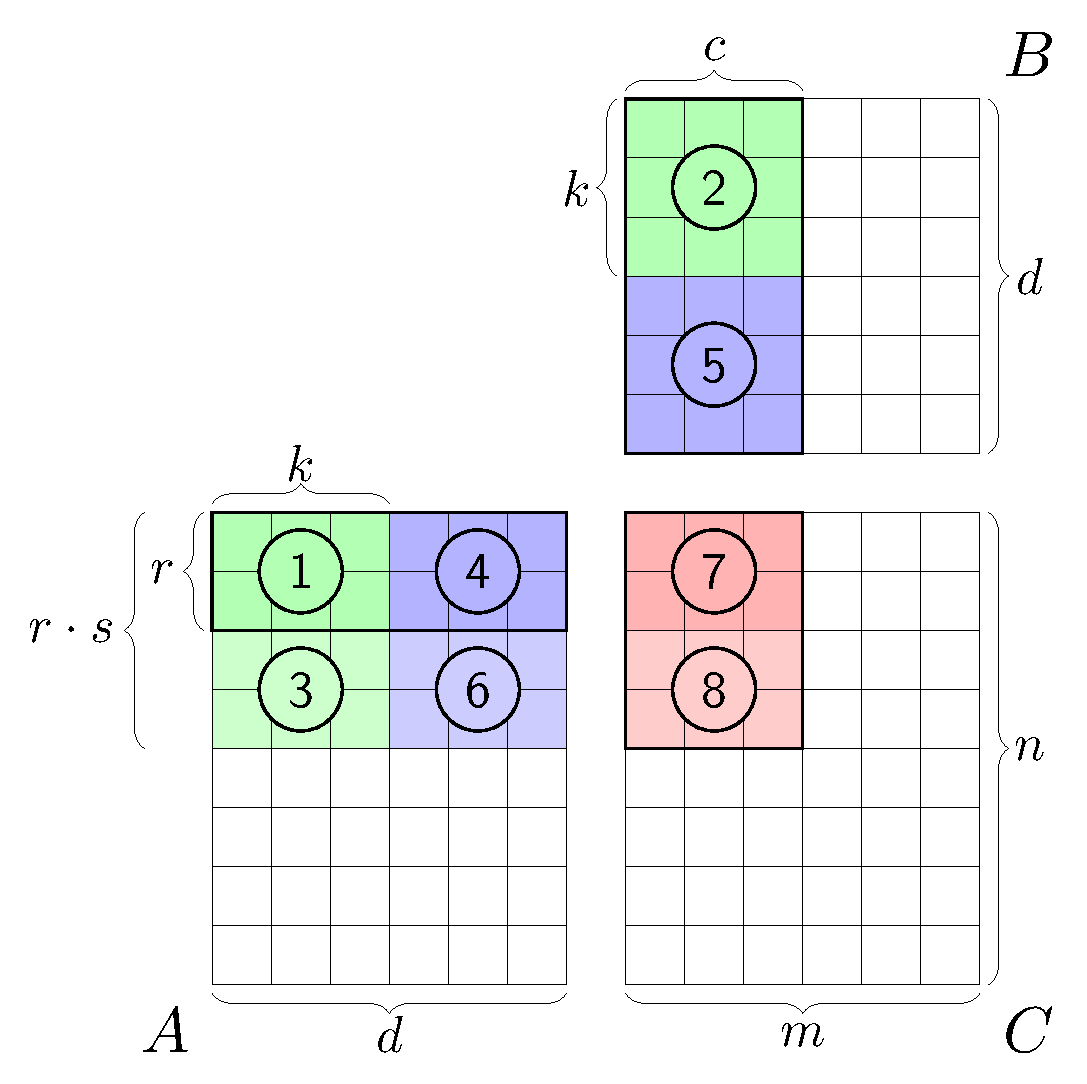
\includegraphics[width=.4\textwidth]{HLPP/memory_access}
  \caption{Implementation schema of the specialized allpairs skeleton.}
  \label{fig:memory_access}
\end{figure}
For the allpairs skeleton with the zip-reduce customizing function, we can adopt the implementation schema for GPUs~\cite{SaA-13}, as shown in Figure~\ref{fig:memory_access}.
We allocate two arrays in the local memory, one of size $r\times k$ ($r=2$, $k=3$ in Figure~\ref{fig:memory_access}) for elements of $A$ and one of size $k\times c$ ($c=3$ in Figure~\ref{fig:memory_access}) for elements of $B$.
A work-group consisting of $c\times r$ work-items computes $s$ blocks ($s=2$ in Figure~\ref{fig:memory_access}) of the result matrix $C$.
In Figure~\ref{fig:memory_access}, the two blocks marked as \circled{7} and \circled{8} are computed by the same work-group as follows.
In the first iteration, the elements of blocks \circled{1} and \circled{2} are loaded into the local memory and combined following the zip-reduce pattern.
The obtained intermediate result is stored in block \circled{7}.
Then, the elements of block \circled{3} are loaded and combined with the elements from \circled{2} which still reside in the local memory.
The intermediate result is stored in block \circled{8}.
In the second iteration, the algorithm continues in the same manner with blocks \circled{4}, \circled{5}, and \circled{6}, but this time, the elements of the blocks are also combined with the intermediate results of the first iteration, which are stored in blocks \circled{7} and \circled{8}.
The advantage of computing multiple blocks by the same work-group is that we keep the elements of $B$ in the local memory when computing the intermediate results, i.\,e., we do not reload block \circled{2} twice for the computation of blocks \circled{7} and \circled{8}.

Every element loaded from the global memory is used by multiple work-items:
e.\,g., the upper left element of block \circled{1} is loaded only once from the global memory, but used three times:
in the computation of the upper left, upper middle, and upper right elements of \circled{7}.
In general, every element loaded from $A$ is reused $c$ times, and every element from $B$ is reused $r\cdot s$ times.
As the intermediate results are stored in the global memory of matrix $C$, we perform two additional memory accesses (read/write) for every iteration, i.\,e., $2\cdot \frac{d}{k}$ in total.
Therefore, instead of $n\cdot m\cdot (d + d + 1)$ global memory accesses necessary when not using the local memory, only $n\cdot m\cdot (\frac{d}{r\cdot s} + \frac{d}{c} + 2\cdot \frac{d}{k})$ global memory accesses are performed.
By increasing the parameters $s$ and $k$, or the number of work-items in a work-group ($c$ and $r$), more global memory accesses can be saved.
However, the work-group size is limited by the GPU hardware.
While the parameters can be chosen independently of the matrix sizes, we have to consider the amount of available local memory.
\cite{SaA-13}~discusses how suitable parameters can be found by performing runtime experiments.

\begin{figure}[b]
  \centering
  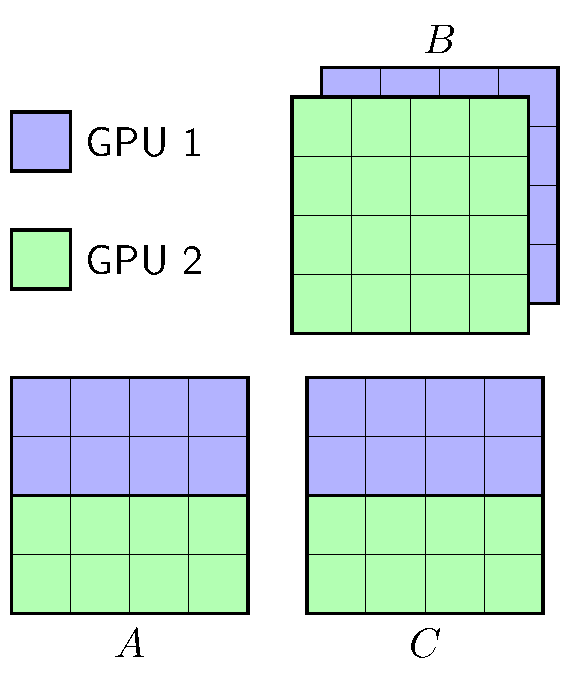
\includegraphics[width=.3\textwidth]{HLPP/multi_gpu}
  \caption{Data distributions used for a system with two GPUs: matrices $A$ and $C$ are block distributed, matrix $B$ is copy distributed.}
  \label{fig:multi_gpu}
\end{figure}

\section{The Allpairs Skeleton using Multiple GPUs (HLPP)}
\label{sec:multi_gpu}
The allpairs skeleton can be efficiently implemented not only on systems with a single GPU, but on multi-GPU systems as well.
The SkelCL library provides four \emph{data distributions} which specify how a container data type (vector or matrix) is distributed among multiple GPUs~\cite{StKG-12}.
We use two of them in our multi-GPU implementation of the allpairs skeleton, as shown in Figure~\ref{fig:multi_gpu}:
Matrix $B$ is \emph{copy} distributed, i.\,e., it is copied entirely to all GPUs in the system.
Matrix $A$ and $C$ are \emph{block} distributed, i.\,e., they are row-divided into as many equally-sized blocks as GPUs are available;
each block is copied to its corresponding GPU.
Following these distributions, each GPU computes one block of the result matrix $C$.
In the example with two GPUs shown in Figure~\ref{fig:multi_gpu}, the first two rows of $C$ are computed by GPU 1 and the last two rows by GPU 2.
The allpairs skeleton automatically selects these distributions; therefore, no changes to the already discussed implementations of the matrix multiplication are necessary for using multiple GPUs.
\from{HLPP end}


\from{PaCT begin}



\subsection{The MapOverlap Skeleton}
\label{sec:skelcl:mapoverlap}
% ------------------------------------------------------------------------------
Many numerical and image processing applications dealing with two-dimensional data perform calculations for a particular data element (e.\,g., a pixel) taking neighboring data elements into account.
To facilitate the development of such applications, we define in SkelCL a skeleton that can be used with both vector and matrix data type; we explain the details for the matrix data type.
\begin{itemize}
  \item The \emph{MapOverlap} skeleton takes two parameters: a unary function $f$ and an integer value $d$.
   It applies $f$ to each element of an input matrix $m_{in}$ while taking the neighboring elements within the range $[-d, +d]$ in each dimension into account, i.\,e.
  \begin{align*}
m_{out}[i,j]=f\left(
\begin{array}{ccccc}
m_{in}[i-d,j-d] & \hdots & m_{in}[i-d,j] & \hdots & m_{in}[i-d,j+d] \\
\vdots & ~ & \vdots & ~ & \vdots \\
m_{in}[i,j-d] & \hdots & m_{in}[i,j] & \hdots & m_{in}[i,j+d]\\
\vdots & ~ & \vdots & ~ & \vdots \\
m_{in}[i+d,j-d] & \hdots & m_{in}[i+d,j] & \hdots & m_{in}[i+d,j+d] \\
\end{array}
\right)
\end{align*}
\end{itemize}

In the actual source code, the application developer provides the function $f$ which receives a pointer to the element in the middle, $m_{in}[i,j]$.

\begin{lstlisting}[%
caption={MapOverlap skeleton computing the sum of all direct neightbors for every element in a matrix},%
float=bp,%
label={lst:mapoverlap01}]
MapOverlap<float(float)> m("float func(float* m_in){
float sum = 0.0f;
for (int i = -1; i < 1; ++i)
	for (int j = -1; j < 1; ++i)
 		sum += get(m_in, i, j); return sum;
}", 1, SCL_NEUTRAL, 0.0f);
\end{lstlisting}


Listing~\ref{lst:mapoverlap01} shows a simple example of computing the sum of all direct neighboring values using the MapOverlap skeleton.
To access the elements of the input matrix $m_{in}$, function \texttt{get} is provided by SkelCL.
All indices are specified relative to the middle element $m_{in}[i,j]$; therefore, for accessing this element the function call \texttt{get(m\_in, 0, 0)} is used.
The application developer must ensure that only elements in the range specified by the second argument $d$ of the MapOverlap skeleton, are accessed.
In Listing~\ref{lst:mapoverlap01}, range is specified as $d=1$, therefore, only direct neighboring elements are accessed.
To enforce this property, boundary checks are performed at runtime by the \texttt{get} function.
In future work, we plan to avoid boundary checks at runtime by statically proving that all memory accesses are in bounds, as it is the case in the shown example.


Special handling is necessary when accessing elements out of the boundaries of the matrix, e.g., when the item in the top-left corner of the matrix accesses elements above and left of it.
The MapOverlap skeleton can be configured to handle such out-of-bound memory accesses in two possible ways:
1) a specified neutral value is returned;
2) the nearest valid value inside the matrix is returned.
In Listing~\ref{lst:mapoverlap01}, the first option is chosen and $0.0$ is provided as neutral value.

\begin{lstlisting}[%
caption={An OpenCL kernel performing the same calculation as the MapOverlap skeleton shown in Listing~\ref{lst:mapoverlap01}.},%
float=tbp,%
label={lst:raw_opencl01}]
__kernel void sum_up(__global float* m_in,
                     __global float* m_out,
                     int width, int height) {
  int i_off = get_global_id(0); 
  int j_off = get_global_id(1);
  float sum = 0.0f;
  for (int i = i_off - 1; i < i_off + 1; ++i)
    for (int j = j_off - 1; j < j_off + 1; ++j) {
      // perform boundary checks
      if ( i < 0 || i > width || j < 0 || j > height )
        continue;
      sum += m_in[ j * width + i ];     }
  m_out[ j_off * width + i_off ] = sum; }
\end{lstlisting}


Listing~\ref{lst:raw_opencl01} shows how the same simple calculation can be performed in standard OpenCL.
While the amount of lines of code increases by a factor of 2, the complexity of each single line also increases:
1) Besides a pointer to the output memory, the width of the matrix has to be provided as parameter; 2) the correct index has to be calculated for every memory access using an offset and the width of the matrix, i.\,e.
knowledge about how the two-dimensional matrix is stored in one-dimensional memory is required.
3) In addition, manual boundary checks have to be performed to avoid faulty memory accesses. 

SkelCL avoids all these low-level details.
Neither additional parameter, nor index calculations or manual boundary checks are necessary.

\subsection{The Allpairs Skeleton}
\label{sec:all-pairs_skeleton}

\emph{All-pairs computations} occur in a variety of applications, ranging from pairwise Manhattan distance computations used in bioinformatics~\cite{DaDQR-09} to N-Body simulations used in physics~\cite{ArSV-09}.
All these applications follow a common computational scheme:
for two sets of entities, the same computation is performed independently for all pairs of entities from the first set combined with entities from the second set.
An entity is usually described by a $d$-dimensional vector.

We define the all-pairs computation scheme for two sets of $n$ and $m$ entities, each entity represented by a $d$-dimensional vector.
We represent the sets as an $n\times d$ matrix $A$ and an $m\times d$ matrix $B$.
The all-pairs computation yields an output matrix $C$ of size $n\times m$ as follows:
$C_{i, j} = A_i \oplus B_j$, where $A_i$ and $B_j$ are rows of $A$ and $B$, correspondingly:
$A_i = [A_{i,1}, \cdots, A_{i, d}]$, $B_j = [B_{j,1}, \cdots, B_{j,d}]$,
and $\oplus$ is a binary function applied to every pair of rows from $A$ and $B$.

Figure~\ref{fig:allpairs_access} illustrates this definition:
the element marked as \circled{3} of matrix $C$ is computed by combining the second row of $A$ marked as \circled{1} with the third row of $B$ marked as \circled{2} using the binary operator $\oplus$.
\begin{figure}[tb]
  \centering
  \includegraphics[width=0.4\textwidth]{PaCT/allpairs_access_pattern_alternative}
  \caption{The allpairs computation: Element $c_{2,3}$ 
    (\protect\tikz[baseline=(char.base)]\protect\node[shape=circle,draw,inner sep=1pt] (char) {3};)
    is computed by combining the second row of $A$
    (\protect\tikz[baseline=(char.base)]\protect\node[shape=circle,draw,inner sep=1pt] (char) {1};)
    with the third row of $B$
    (\protect\tikz[baseline=(char.base)]\protect\node[shape=circle,draw,inner sep=1pt] (char) {2};)
    using the binary operator $\oplus$}
  \label{fig:allpairs_access}
\end{figure}

For formally defining the all-pairs skeleton, let $d$, $m$ and $n$ be positive numbers.
  Let $A$ be a $n\times d$ matrix, $B$ be a $m\times d$ matrix and $C$ be a $n\times m$ matrix with their entries $a_{i,j}$, $b_{i,j}$ and $c_{i,j}$ respectively.
  Let $\oplus$ be a binary function on vectors. % $\oplus: A \times B \to C$.
  The algorithmic skeleton $allpairs$ is defined as follows:
  \[
	  allpairs(\oplus)\left(\DottedMatrix{a_{1,1}}{a_{1,d}}{a_{n,1}}{a_{n,d}},%
	                           \DottedMatrix{b_{1,1}}{b_{1,d}}{b_{m,1}}{b_{m,d}}\right)%
  	\eqdef \DottedMatrix{c_{1,1}}{c_{1,m}}{c_{n,1}}{c_{n,m}}
  \]
  with entries $c_{i,j}$ of the computed $n\times m$ matrix $C$ defined as:
  \[
	  c_{i,j} = \DottedVector{a_{i,1}}{a_{i,d}} \oplus \DottedVector{b_{j,1}}{b_{j,d}}
  \]

To illustrate the definition, we show how matrix multiplication can be expressed using the allpairs skeleton.

\paragraph{Example 1:}
The matrix multiplication is a basic linear algebra operation, which is a building block of many scientific applications.
A $n\times d$ matrix $A$ is multiplied by a $d\times m$ matrix $B$, producing a $n\times m$ matrix $C=A\times B$ whose element $C_{i,j}$ is computed as the dot product of the $i$th row of $A$ with $j$th column of $B$.
The dot product of two vectors $a$ and $b$ of length $d$ is computed as:
\begin{equation}
  dotProduct(a,b) = \sum_{k=1}^d a_k \cdot b_k
\end{equation}
The matrix multiplication can be expressed using the allpairs skeleton as:
\begin{equation}
  A\times B = allpairs(dotProduct)\left(A, B^T\right)
  \label{eq:mat_mult_allpairs}
\end{equation}
where $B^T$ is the transpose of matrix $B$.
\from{PaCT end}






\from{HiStencils begin}
\section{The SkelCL Skeleton Library (HiStencils)}
\label{sec:skelcl}

\section{New Skeletons for Stencils (HiStencils)}
\label{sec:stencil}

The idea of our approach is that while the stencil operation varies for different applications, the overall structure of stencil computations stays the same.
Therefore, stencil computations can be implemented as a skeleton which is customized by the application developer with a particular stencil operation and particular stencil shape.

To simplify the development of stencil applications, we introduce two specialized skeletons in SkelCL: \emph{MapOverlap} and \emph{Stencil}.
While MapOverlap supports simple stencil computations, the Stencil skeleton provides support for more complex stencil computations with more complex stencil shapes and (possibly) iterative execution.

Listing~\ref{lst:mapoverlap01} shows the implementation of the Sobel edge detection using the \emph{MapOverlap} skeleton.
The MapOverlap skeleton applies a given function $func$ (defined in lines 2--6) to each element of an input matrix $in_{img}$ while taking the neighboring elements within the range $[-d, +d]$ in each dimension into account.
Here, $d$ is the second parameter (line 7) and two additional parameters define how the skeleton handles out-of-bound memory accesses (line 8).
A helper function (\code{get}) is used to easily access the neighboring elements.
The indexes are specified relative to the current element, e.\,g. to access the element on the left the function call \code{get(in, -1, 0)} is used.

Special handling is necessary when accessing elements out of the boundaries of the matrix, e.g., when the item in the top-left corner of the matrix accesses elements above and left of it.
The MapOverlap skeleton can be configured to handle such out-of-bound memory accesses in two possible ways:
1) a specified neutral value is returned;
2) the nearest valid value inside the matrix is returned.
In Listing~\ref{lst:mapoverlap01}, the first option is chosen and $0$ is provided as neutral value.

\begin{lstlisting}[%
caption={Implementation of Sobel edge detection using the MapOverlap skeleton},%
float=tbp,%
label={lst:mapoverlap01}]
MapOverlap<char(char)> sobel(
 "char func(const char* in_img) {
    char ul = get(in_img, -1, -1);
    ...
    char lr = get(in_img, +1, +1);
    return computeSobel(ul,..., lr);}",
 1, Padding::NEUTRAL, 0);

output = sobel(input);
\end{lstlisting}

Simple stencil computations with a regular stencil shape can easily be expressed using the MapOverlap skeleton.
For more complex stencil computations, e.\,g. iterative stencils, we introduce the more advanced \emph{Stencil} skeleton.
\paragraph{The MapOverlap Skeleton}

Listing~\ref{lst:stencil01} shows the implementation of an iterative stencil application simulating heat transfer.
This application simulates heat spreading from one location and flowing throughout a two-dimensional simulation space.
\begin{lstlisting}[%
caption={Implementation of heat simulation using the Stencil skeleton},%
float=tbp,%
label={lst:stencil01}]
Stencil<char(char)> heatSim(
 "char func(const char* in) {
    char lt = get(in, -1, -1);
    char lm = get(in, -1,  0);
    char lb = get(in, -1, +1);
    return computeHeat(lt, lm, lb); }",
 StencilShape(1, 0, 1, 1),
 Padding::NEUTRAL, 255);

output = heatSim(100, input);
\end{lstlisting}


The application developer specifies the function (line 2--6) describing the computation and, therefore, the stencil shape, as well as the stencil shape's extents (line 7) and the out-of-bound handling (line 8).
The stencil shape's extents are specified using four values for each of the directions:
up, right, down, left.
In the example in Listing~\ref{lst:stencil01}, the heat flows from left to right, therefore, no accesses to elements to the right are necessary and the stencil space's extents are specified accordingly (note the $0$ in line 7 representing the extent to the right).
Figure~\ref{fig:stencilShape} illustrates this situation: the dark gray element is updated by using the values from the left.
The specified stencil shape's extent is highlighted in light gray.
In our current implementation, the user has to explicitly specify the stencil shape's extents, which is necessary for performing the out-of-bound handling on the GPU.
In future work, we plan to automatically infer the stencil shape's extents
from the customizing function using source code analysis in order to free the user from specifying this information explicitly.
\begin{figure}
  \begin{centering}
    \includegraphics[width=.18\textwidth]{HiStencils/heat_transfer}
    \caption{Stencil shape for heat transfer simulation}
    \label{fig:stencilShape}
    \vspace{-.5em}
  \end{centering}
\end{figure}

Many stencil applications apply a stencil multiple times for a fixed number of iterations, or until a certain condition is met.
For example, to iterate the heat transfer simulation for one hundred steps, we specify the number of iterations to perform when executing the skeleton (line 10).
In the future, we plan to allow the user to specify a custom function which checks a condition to stop the iterations.

The MapOverlap skeleton can be configured to handle out-of-bounds accesses by returning the nearest valid value of the input matrix.
Another distinction can be made regarding iterations and sequences of stencil operations:
using elements of the \textbf{initial}, user-provided input matrix or using elements of the \textbf{current} step's input matrix, which already was updated during earlier stencil operations.
The Stencil skeleton can be configured to handle out-of-bounds accesses in both ways, thus offering three possible ways, including the neutral value. 
For each of them, there is an own kernel function, loading appropriate elements into local memory. 

\paragraph{The Stencil Skeleton}

\paragraph{Sequence of Stencil Operations}
Many real-world applications perform different stencil operations in a sequence.
Let us consider the popular \emph{Canny algorithm} which is used for detecting edges in images.
For the sake of simplicity we consider a simplified version, which applies the following stencil operations in a sequence:
first, a noise reduction operation is applied, e.g., a Gaussian filter;
second, an edge detection operator like the Sobel filter is applied;
third, the so-called non-maximum suppression is performed, where all pixels in the image are colored black except pixels being a local maximum;
finally, a threshold operation is applied to produce the final result.
A more complex version of the algorithm performs the edge tracking by hysteresis, as an additional step.
This results in detecting some weaker edges, but even without this
additional step the algorithm usually achieves good results.

In SkelCL, each single step of the Canny algorithm can be expressed using the Stencil skeleton.
The last step, threshold operation, does not need access to neighboring elements, as the user threshold function only checks the value of the current pixel.
Therefore, this step can be expressed using SkelCL's simpler Map skeleton.
The Stencil skeleton's implementation automatically uses the simpler Map skeleton's implementation when the user specifies a stencil shape which extents are $0$ in all directions.

\begin{lstlisting}[%
  caption={Structure of the Canny algorithm as implemented with a sequence of skeletons.},%
  float=tbp,%
  label={lst:canny01}]
Stencil<Pixel(Pixel)> gauss(...);
Stencil<Pixel(Pixel)> sobel(...);
Stencil<Pixel(Pixel)> nms(...);
Stencil<Pixel(Pixel)> threshold(...);

StencilSequence<Pixel(Pixel)> canny(
  gauss, sobel, nms, threshold);

output = canny(1, input);
\end{lstlisting}

To implement the Canny algorithm in SkelCL, the single steps can be combined as shown in Listing~\ref{lst:canny01}.
The individual steps are defined in lines 1--4 and then combined to a sequence of stencils in line 6 and 7.
During execution (line 9), the stencil operation are performed in the order which is specified when creating the \emph{StencilSequence} object.

\paragraph{Implementation}
In order to achieve high performance, our implementations of both the MapOverlap and the Stencil skeleton use the GPU's fast local memory.
Both implementations perform the same basic steps on the GPU:
first, the data is loaded from the global memory into the local memory;
then, the user-defined function is called for every data element by passing a pointer to the element's location in the local memory;
finally, the result of the user-defined function is copied back into the global memory.

Although both implementations perform the same basic steps, different strategies are implemented for loading the data from the global into the local memory.

\begin{figure}
  \begin{centering}
    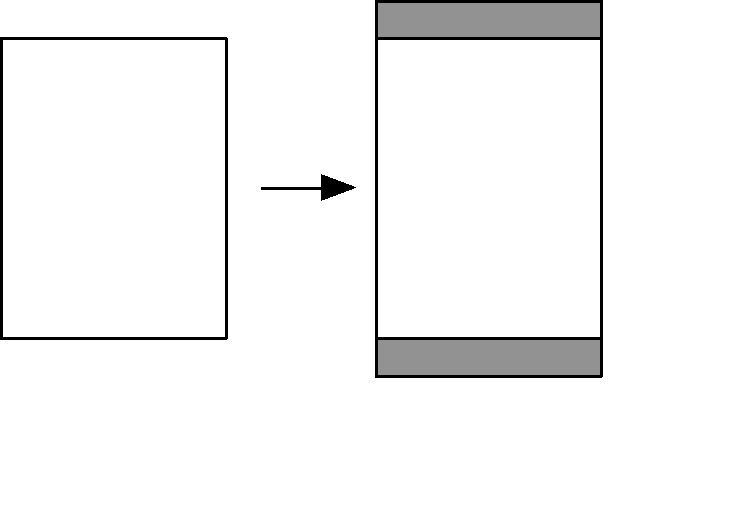
\includegraphics[width=.29\textwidth]{HiStencils/map_overlap}
    \caption{The MapOverlap skeleton prepares a matrix by copying data on the top and bottom.}
    \label{fig:preparation}
    \vspace{-.5em}
  \end{centering}
\end{figure}

The MapOverlap skeleton prepares the input matrix on the CPU before uploading it to the GPU:
padding elements are appended; they are used to avoid out-of-bounds memory accesses to the top and bottom of the input matrix, as shown in Figure~\ref{fig:preparation}.
This slightly enlarges the input matrix, but it reduces branching on the GPU due to avoiding some out-of-bound checks.
In SkelCL a matrix is stored row-wise in memory on the CPU and GPU, therefore, it would be complex and costly to add padding elements on the left and right of the matrix.
To avoid out-of-bound accesses for these regions, the boundary checks are performed on the GPU.

The Stencil skeleton has to use a different strategy in order to enable the usage of different padding modes and stencil shapes when using several Stencil skeletons in a sequence.
As an example, consider two stencil shapes in a sequence where the first shape defines a neutral element $0$ and the second defines a neutral element $1$.
This cannot be implemented using MapOverlap's implementation strategy.
Therefore, Stencil does not append padding elements on the CPU, but rather manages all out-of-bounds accesses on the GPU, which slightly increases branching.

\section{Targeting Multi-GPU Systems (HiStencils)}
\label{sec:multi_gpu}
The implicit and automatic support of systems with multiple OpenCL devices is one of the key features of SkelCL.
By using distributions, SkelCL completely liberates the user from error-prone and low-level explicit programming of data (re)distributions on multiple GPUs. 

The MapOverlap skeleton uses the overlap distribution with \textit{border regions} in which the elements calculated by a neighboring device are located.
When it comes to iteratively executing a skeleton, data has to be transferred among devices between iteration steps, in order to ensure that data for the next iteration step is up-to-date.
As the MapOverlap skeleton does not explicitly support iterations, its implementation is not able to exchange data between devices besides a full down- and upload of the matrix.
In addition, data exchange has to be performed after each iteration.
We can enlarge the number of elements in the border regions and perform multiple iteration steps on each device before exchanging data.
However, this introduces redundant computations, such that a trade-off between data exchange and redundant computations has to be found.
 
For the Stencil skeleton, the user can specify the number of iterations between \textit{device synchronisations}, where all border regions are updated with elements from the corresponding inner border regions of the neighboring device.
The border regions are sized by default in such a way that the specified number of iterations can be performed without leading to incorrect results.
However, there may be cases in which a different number of iterations between device synchronizations may result in better performance.
Therefore, Stencil offers the user the possibility to specify that number.
Please note that the implementation of the Stencil skeleton only exchanges elements from the border region and does not perform a full down- and upload of the matrix, as the MapOverlap skeleton does.

Figure \ref{fig:syncDevices} shows the device synchronization.
Only the appropriate elements in the inner border region are downloaded and stored as \texttt{std::vector}s in a \texttt{std::vector}.
Within the outer vector, the inner vectors are swapped pair-wise on the host, so that the inner border regions can be uploaded in order to replace the out-of-date border regions.

For the first iteration after a device synchronization, there are as many work-items on the GPU active as there are total elements on the device.
As the first and last rows of the border regions become invalid within an iteration, the corresponding work-items become inactive in the following iteration step.
This is done by using an offset and by reducing the number of total work-items when launching the OpenCL kernel.
The Stencil's four kernel functions (one for each out-of-bounds handling mode and one for the adapted Map skeleton) can be used for both single- and multi-GPU systems.
 
\begin{figure}[tb]
	\centering
	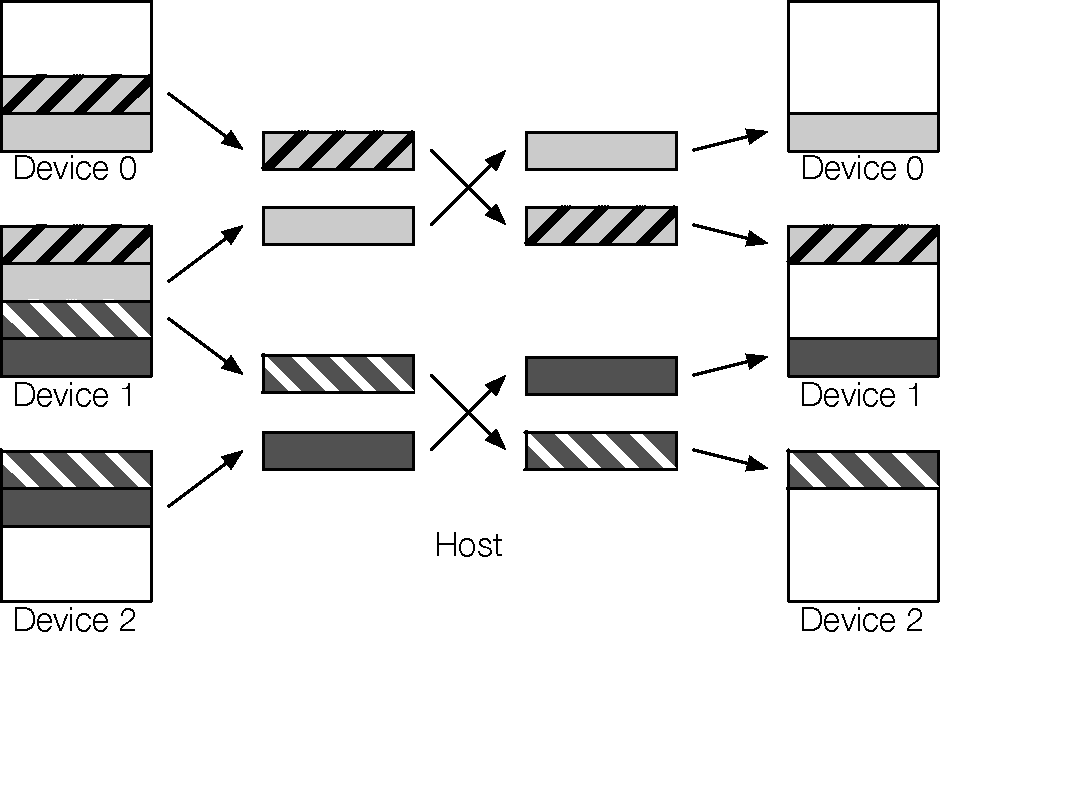
\includegraphics[width=\columnwidth]{HiStencils/data_exchange}
	\caption{\small Device synchronization for three devices. Equally patterned and colored chunks represent the border regions and their matching inner border region. After the download of the appropriate inner border regions, they are swapped pair-wise on the host. Then the inner border regions are uploaded in order to replace the out-of-date border regions.}
	\label{fig:syncDevices}
  \vspace{1em}
\end{figure} 
\from{HiStencils end}


% Chapter 4: Application Studies
\chapter{Application Studies}
\label{chapter:skelcl-evaluation}

In this chapter we present various application studies evaluating the usefulness and performance of the abstractions introduced by the \SkelCL programming model which was presented in the previous section.
We start with a brief discussion of the experimental setup used throughout the chapter and discuss the metrics used to evaluate the \SkelCL programming model.
We will then look at applications from a wide range of application domains ranging from simple benchmark applications like the computation of the Mandelbrot set, over linear algebra and image processing applications, to real-world applications in medical imaging, physics, and biology.

For all application source codes using the \SkelCL library which are presented in this section we only show relevant sections and omit implementation details like initializing \SkelCL, including the correct set of header files, and prefix names with the \code{skelcl} namespace.

\section{Experimental Setup}
\label{sec:skelcl:experimental_setup}
This section briefly discusses the evaluation metrics used in this chapter which were chosen to measure the quality of the abstractions introduced in the \SkelCL programming model and their implementation in the \SkelCL library.
We will also discuss the hardware used in the experiments.


\subsection{Evaluation Metrics}
We want to evaluate the programmability, \ie, the ease of programming, and performance of the \SkelCL programming model and library.

Directly measuring programmability is difficult.
Various studies~\cite{HochsteinCSAB2005,HochsteinBVG2008} have been conducted and metrics~\cite{VanderwielNL1997} have been proposed to measure how convenient a certain style of programming or a certain programming model is.
None of these metrics is widely established in the scientific or industrial communities.
We chose to use one of the simples metrics possible to quantify programming effort: counting the \emph{Lines Of source Code} (LOC).
The author wants to emphasize that this metric is not always a good representation of programmability.
A shorter program does not necessarily mean that the development of the program has been more convenient.
We will, therefore, alongside presenting the lines of code argue \emph{why} the programming of parallel devices, like \GPUs, is easier as compared to the state-of-the-art approaches CUDA and OpenCL.
% These discussions will argue that code written using the \SkelCL programming approach has, besides ease of programming, other properties of high quality software including:
% high level of re-use, portability, 

As the metric for performance we use absolute and relative runtime.
%-- where possible --
We only make comparisons using software executed on the same hardware.
We perform comparisons using published software from researchers or officially provided by NVIDIA or AMD.
In addition, we use self developed and optimized CUDA and OpenCL code for comparisons versus the code written using the \SkelCL library.

\subsection{Hardware Setup}
For performing our runtime experiments we used a PC equipped with a quad-core \CPU (Intel Xeon E5520, 2.26\,GHz) and 12\,GB of main memory.
The system is connected to a Nvidia Tesla S1070 computing system consisting of four Nvidia Tesla \GPUs.
The S1070 has 16\,GB of dedicated memory (4\,GB per \GPU) which is accessed with up to 408\,GB/s (102\,GB/s per \GPU).
Each \GPU comprises 240 streaming processor cores running at up to 1.44\,GHz.
The Linux based Ubuntu operating system was used.
The runtime experiments where conducted at different times from 2010 until 2015.
For each experiment the latest Nvidia \GPU driver available was used.

This hardware setup represents a common heterogeneous system comprising four \CPU cores and 960 \GPU streaming processor cores with a total of 28\,GB of memory.
Overall this system has a theoretical single-precision floating point performance of 4219.52 GFLOPS (4 $\times$ 1036.8 GFLOPS for the \GPUs and 72.32 GFLOPS for the \CPU).



\section{Computation of the Mandelbrot Set}

\begin{figure}[tb]
  \centering
  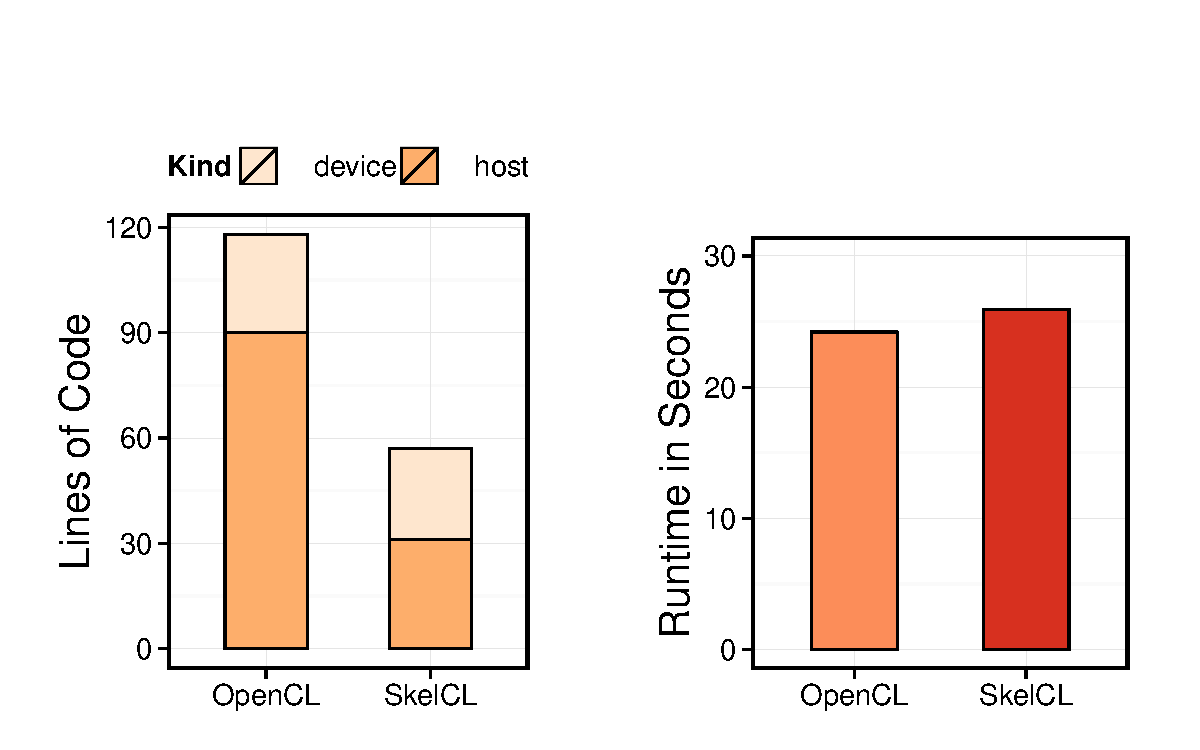
\includegraphics[width=.75\textwidth]{mandelbrot}
  \caption{Visualization of a part of the Mandelbrot set. The image was produced using the \SkelCL library.}
  \label{fig:mandelbrot}
\end{figure}

The Mandelbrot~\cite{Mandelbrot1980} set includes all complex numbers $c \in {\mathbb C}$ for which the sequence
\begin{equation}
	z_{i+1} = z_{i}^{2} + c,\qquad i\in {\mathbb N}
	\label{eq:mandelbrot}
\end{equation}
starting with $z_{0}=0$ does not escape to infinity.
When drawn as an image with each pixel representing a complex number, the boundary of the Mandelbrot set forms a fractal.
\autoref{fig:mandelbrot} shows an image visualizing part of the Mandelbrot set.
The software producing the image was implemented using the \SkelCL library. 
The calculation of such an image is a time-consuming task, because the sequence given by~\autoref{eq:mandelbrot} has to be calculated for every pixel.
If this sequence does not cross a given threshold for a given number of iteration steps, it is presumed that the sequence will converge.
The respective pixel is thus taken as a member of the Mandelbrot set, and it is displayed black.
Other pixels outside are assigned a color that corresponds to the number of iterations of the sequence given by~\autoref{eq:mandelbrot}.
Computing a Mandelbrot fractal is easily parallelizable, as all pixels of the fractal can be computed simultaneously.

\subsubsection*{\SkelCL Implementation}
\label{sec:mandelbrot:implementation}
The \SkelCL implementation of the Mandelbrot set computations uses the \map skeleton as shown in \autoref{eq:skelcl:mandelbrot}.
\begin{align}
  mandelbrot\ w\ h =&  \nonumber\\
         map\ compute&ColorOfPixel\ (generateIndex\ w\ h)
  \label{eq:skelcl:mandelbrot}
\end{align}
\todo{Explain $generateIndex$ and connection to \ref{eq:mandelbrot}}
Here function $mandelbrot$ is defined taking two arguments -- the width $w$ and height $h$ of the image to compute.
The function is defined in terms of the \map skeleton customized with $computeColorOfPixel$ computing the color of a single pixel of the image (not shown here) and operating on an input matrix of size $w\times h$ consisting of indices.

The implementation using the \SkelCL library is shown in \autoref{lst:skelcl:mandelbrot}.
A user-defined data type is introduced to represent the color of a pixel (line~\ref{lst:skelcl:mandelbrot:pixel}).
An instance of the \map skeleton is created in line~\ref{lst:skelcl:mandelbrot:map} and applied to \code{IndexMatrix} (line~\ref{lst:skelcl:mandelbrot:apply}).
The \code{IndexMatrix} represents all indices up to a given width and height.
It is implemented as a special representation of the generic \code{Matrix} class to avoid explicitly storing the indices in memory.
Instead when accessing an element the index value is computed on the fly.
This implementation avoids allocation of memory for storing the indices and transferring them to the \GPU.


\begin{lstlisting}[%                                                             
caption={Implementation of the Mandelbrot set computation in \SkelCL},%
numbers=left,%
float=tb,
label={lst:skelcl:mandelbrot}]
typedef struct { char r; char g; char b; } Pixel;$\label{lst:skelcl:mandelbrot:pixel}$

Pixel computeColorOfPixel(IndexPoint) { ... };

void mandelbrot(const int width, const int height) {
  auto m = map(computeColorOfPixel);$\label{lst:skelcl:mandelbrot:map}$
  auto image = m(IndexMatrix{w, h});$\label{lst:skelcl:mandelbrot:apply}$
  writeToDisk(image); }
\end{lstlisting}

We created two similar parallel implementations for computing a Mandelbrot fractal using CUDA and OpenCL.\todo{Show in appendix?}
We compare the programming effort and performance for these implementations against our \SkelCL implementation.

\subsubsection*{Programming effort}
\label{sec:mandelbrot:programming}

CUDA and \SkelCL require a single line of code for initialization in the host code, whereas OpenCL requires a lengthy initialization of different data structures which takes about 20 lines of code.

The host code differs significantly between all implementations.
In CUDA, the kernel is called like an ordinary function.
A proprietary syntax is used to specify the size of work-groups executing the kernel.
With OpenCL, several API functions are called to load and build the kernel, pass arguments to it and to launch it using a specified work-group size.
In \SkelCL, the \map skeleton is used to compute the color of all pixels in the image.
An \code{IndexMatrix} representing complex numbers, each of which is processed to produce a pixel of the Mandelbrot fractal, is passed to the \map skeleton upon execution.
Specifying the work-group size is mandatory in CUDA and OpenCL, whereas this is optional in \SkelCL.

\paragraph{Program size}
The OpenCL-based implementation has 118 lines of code (kernel: 28~lines, host program: 90~lines) and is thus more than twice as long as the CUDA and \SkelCL versions with 49 lines (28, 21) and 57 lines (26, 31), respectively (see \autoref{fig:mandelbrot_runtime}).
The lengths of the CUDA- and \SkelCL-based implementations differ by only a few lines.

\paragraph{Kernel size}
The kernel function is similar in all implementations: it takes a pixel's position (\ie, a complex number) as input, performs the iterative calculation for this pixel, and returns the pixel's color.
However, while the input positions are given explicitly when using the \map skeleton in SkelCL, no positions are passed to the kernel in the CUDA- and OpenCL-based implementations.
The positions are implicitly determined based on the work-item's index.

\subsubsection*{Performance experiments}
\label{sec:mandelbrot:performance}
\todo{Exclude CUDA ?}

\begin{figure}[tb]
    \centering
    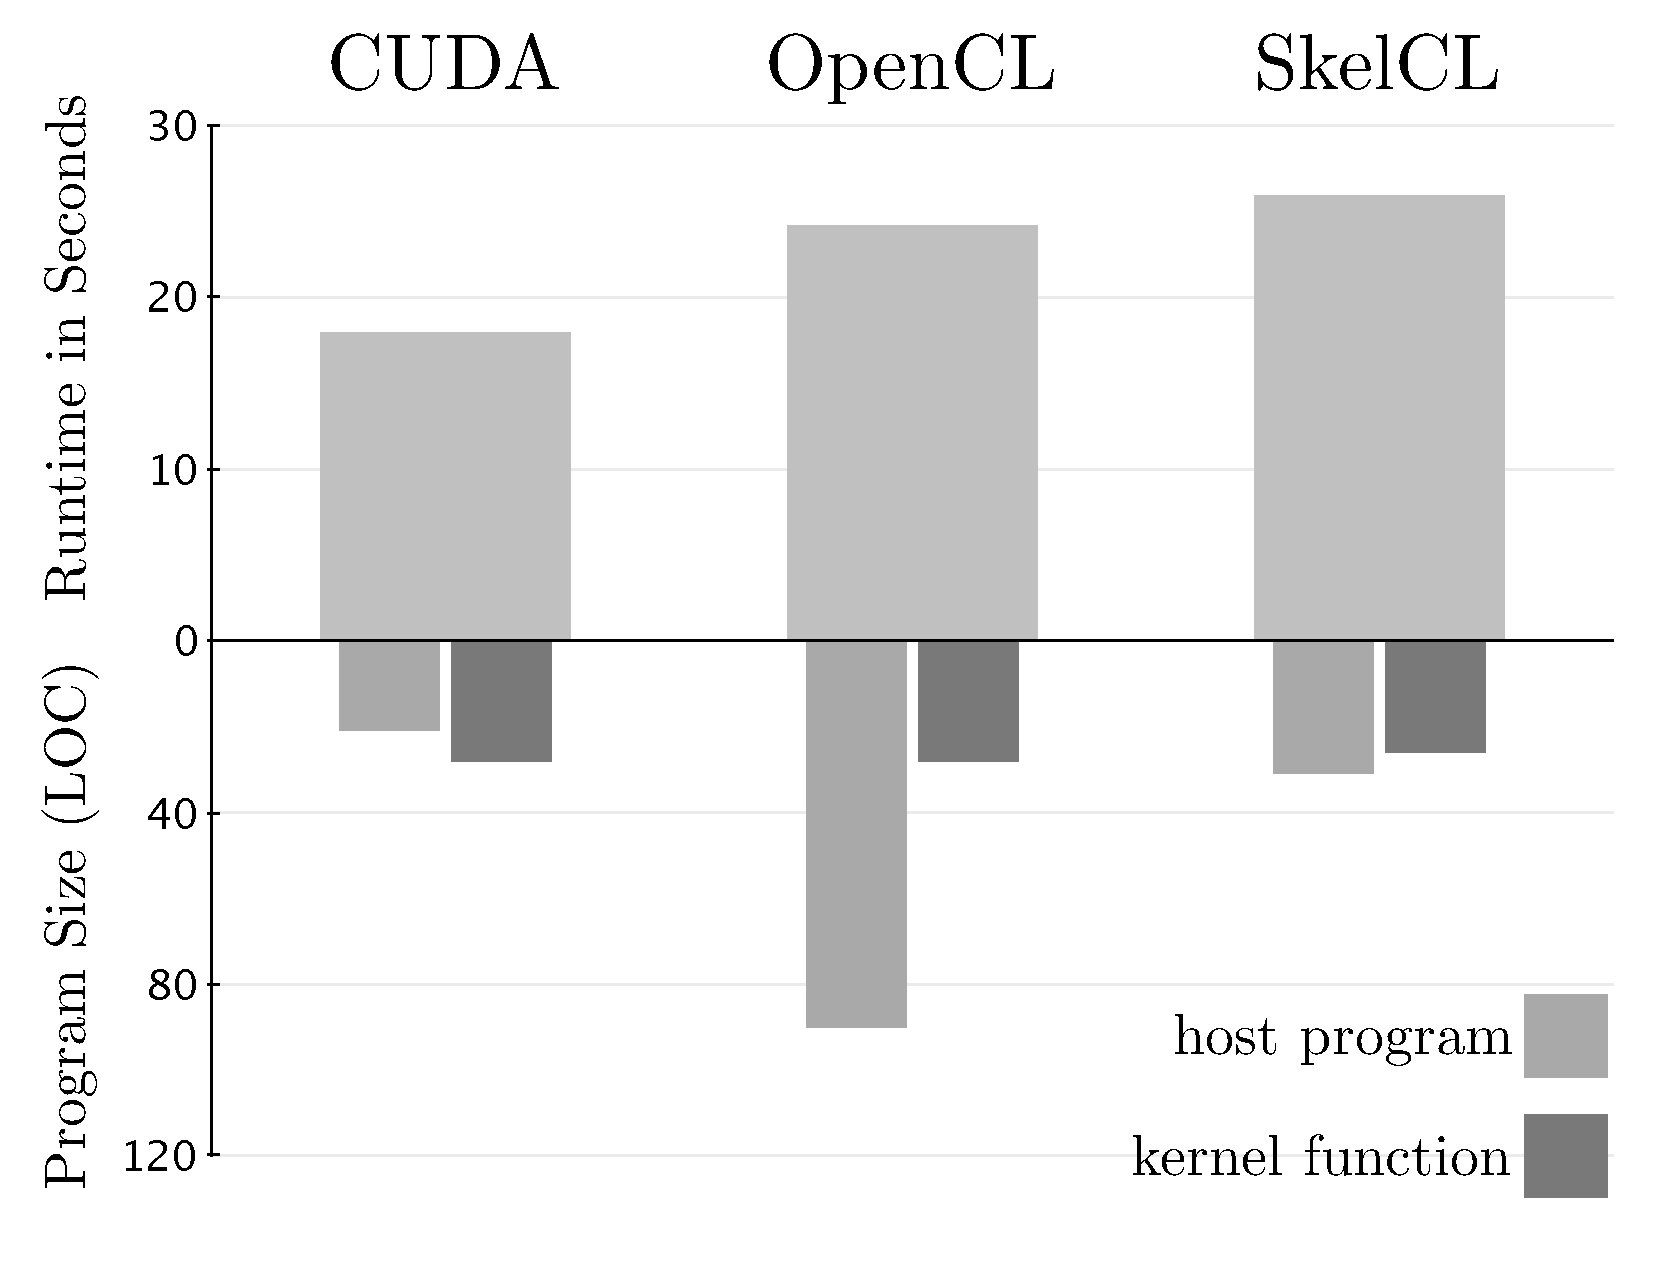
\includegraphics[width=0.6\textwidth]{HIPS/ChartMandelbrot}
    \caption{Runtime and program size of the Mandelbrot application.}
    \label{fig:mandelbrot_runtime}
\end{figure}%


We tested our implementations on a single \GPU of our test system to compute a Mandelbrot fractal of size 4096$\times$3072 pixels.
In CUDA and OpenCL, work-groups of 16$\times$16 are used; \SkelCL uses its default work-group size of~256 work-items.

The results are shown in \autoref{fig:mandelbrot_runtime}.
As compared to the runtime of the \SkelCL-based implementation (26 seconds), the implementation based on OpenCL (25 seconds) and CUDA (18 seconds) are faster by 4\% and 31\%, respectively.
Since \SkelCL is built on top of OpenCL, the performance difference of \SkelCL and OpenCL can be regarded as the overhead introduced by SkelCL.
Previous work~\cite{KongDiYaLiCaStMaZh2010} also reported that CUDA was usually faster than OpenCL, which also explains the higher performance of the implementation based on CUDA.
The Mandelbrot application demonstrates that \SkelCL introduces a tolerable overhead of less than 5\% as compared to OpenCL.
A clear benefit of this overhead is the reduced programming effort required by the SkelCL program.



\section{Linear Algebra Applications}

BLAS ... important building blocks ...
\todo{Write stuff}

\subsection{Sum of absolute values}
\label{sec:asum}
\autoref{eq:asum} shows the mathematical definition of the sum of absolute values (short \emph{asum}) for a vector $\vec{x}$ of length $n$ with elements $x_i$:
\begin{equation}
  asum\ \vec{x} = \sum_{i=0}^{n} | x_i |
  \label{eq:asum}
\end{equation}
For all elements of the vector the absolute values are added up to produce the final scalar result.

\subsubsection*{\SkelCL Implementation}
In the \SkelCL programming model we can express \emph{asum} using the \map and \reduce skeletons as follows:
\begin{align}
  asum\ \vec{x} &= reduce\ (+)\ 0\ \big(\ map\ (|\, .\, |)\ \vec{x}\ \big)\label{eq:asum:skelcl}\\
  \text{where:} \qquad | a | &=
    \left\{
      \begin{array}{r l}
      a & \text{if } a \geq 0\\
      -a & \text{if } a < 0
      \end{array}
    \right.\nonumber
\end{align}

The \map skeleton applies the $abs$ function to each element of the input vector before the \reduce skeleton is used to sum up the elements.

The implementation using the \SkelCL library is shown in \autoref{lst:skelcl:asum}.
In lines~\ref{lst:skelcl:asum:skeletons:start}--\ref{lst:skelcl:asum:skeletons:end} the customized skeletons are defined.
The \map skeleton in \autoref{eq:asum:skelcl} corresponds directly to lines~\ref{lst:skelcl:asum:skeletons:start} and~\ref{lst:skelcl:asum:abs} in \autoref{lst:skelcl:asum} where the $|\, .\, |$ function is represented using a \Cpp lambda expression.
Line~\ref{lst:skelcl:asum:skeletons:end} corresponds directly to the \reduce skeleton in \autoref{eq:asum:skelcl}.
By applying the skeletons to the input vector (line~\ref{lst:skelcl:asum:call}) the result is computed and accessed in line~\ref{lst:skelcl:asum:return}.
In the \SkelCL library implementation the \reduce skeleton returns a vector containing a single element.
The containers in the \SkelCL library are implemented as \emph{futures}~\cite{HewittBa1977,FriedmanWi1978}.
This allows the computation of all skeletons to be performed asynchronously, \ie, when executing a skeleton the computation is launched and the called function returns immediately.
When accessing values of the returned container, \eg, via the array subscript operator as shown in line~\ref{lst:skelcl:asum:return}, the call will block until the accessed value has been computed.

\begin{lstlisting}[%                                                             
caption={Implementation of the \emph{asum} application in \SkelCL},%
numbers=left,%
float=tb,
label={lst:skelcl:asum}]
float asum(const Vector<float>& x) {
  auto absAll = map($\label{lst:skelcl:asum:skeletons:start}$
      [](float a){ if (a >= 0) return a; else return -a; });$\label{lst:skelcl:asum:abs}$
  auto sumUp = reduce([](float a, float b){return a+b;}, 0);$\label{lst:skelcl:asum:skeletons:end}$
  auto result = sumUp( absAll( x ) );$\label{lst:skelcl:asum:call}$
  return result[0]; }$\label{lst:skelcl:asum:return}$
\end{lstlisting}

We compare this implementation against a native OpenCL implementation and an implementation using the CUBLAS library.

\subsubsection*{Programming effort}
\todo{...}

\subsubsection*{Performance experiments}
\todo{...}

As discussed in \autoref{chapter:skelcl} the \SkelCL library implementation generates one (or more) OpenCL kernel for each skeleton.
This procedure makes it difficult to \emph{merge} multiple OpenCL kernels into a single one, which would be required to achieve a competitive performance to the native OpenCL implementation.
In \autoref{ch:fifth}, we will discuss a novel compilation technique addressing this challenge.
This technique supports the generation of a single efficient OpenCL kernel, also for implementing applications like the \emph{asum} example.

\subsection{Dot product}
\label{sec:dot}
The computation of the dot product, \aka scalar product, is a common mathematical operation performed on two input vectors $\vec{x}$ and $\vec{y}$ of identical length $n$ as defined in \autoref{eq:dot_product}:
\begin{equation}
  dotProduct\ \vec{x}\ \vec{y} = \sum_{i=0}^{n} x_i \times y_i
  \label{eq:dot_product}
\end{equation}

\subsubsection*{\SkelCL Implementation}
In \SkelCL we can express $dotProduct$ using the \zip and \reduce skeletons as follows:
\begin{equation}
  dotProduct\ \vec{x}\ \vec{y} = reduce\ (+)\ 0\ \big(\ zip\ (\times)\ \vec{x}\ \vec{y}\ \big)
\end{equation}

The \zip skeleton performs the pairwise multiplication of the input vectors before the \reduce skeleton is used to sum up the intermediate results.

\autoref{lst:skelcl:dot} shows the implementation using the \SkelCL library.
The structure of the implementation is very similar to the \emph{asum} application discussed in \autoref{sec:asum}.
Here we use the \code{front} member function to access the first (and only) element of the computed result vector.

\begin{lstlisting}[%                                                             
caption={Implementation of the dot product application in \SkelCL},%
numbers=left,%
float=tb,
label={lst:skelcl:dot}]
float dotProduct(const Vector<float>& x,
                 const Vector<float>& y) {
  auto mult  = zip([](float x, float y){return x*y;});$\label{lst:skelcl:dot:skeletons:start}$
  auto sumUp = reduce([](float x, float y){return x+y;}, 0);$\label{lst:skelcl:dot:skeletons:end}$
  return sumUp( mult( x, y ) ).front(); }$\label{lst:skelcl:dot:call}$
\end{lstlisting}

\subsubsection*{Programming effort}
\todo{...}

\subsubsection*{Performance experiments}
\todo{...}

\subsection{Matrix Multiplication}

The multiplication of matrices is a basic operation in linear algebra and, therefore, a fundamental building block for many scientific applications.
An $n\times d$ matrix $A$ is multiplied with a $d\times m$ matrix $B$ to produce an $n\times m$ matrix $C$, where the elements of $C$ are computed as:
\begin{equation*}
  C_{ij} = \sum_{k=0}^{d} A_{ik} \times B_{kj}, \qquad \forall\ i \in 1, \ldots, n \wedge j \in 1, \ldots, m
\end{equation*}
Here $A_{i*}$ refers to the $i$th row of $A$ and $B_{*j}$ to the $j$th column of $B$.
\autoref{fig:mm} visualizes this computation.
To compute the highlighted element in matrix $C$, the highlighted row of matrix $A$ is combined with the highlighted column of matrix $B$.
For computing the entire matrix $C$, \emph{all pairs} of rows from $A$ and columns of $B$ have to be processed.
Therefore, in \SkelCL the \allpairs skeleton can be used to express matrix multiplication.

\begin{figure}[tb]
  \centering
  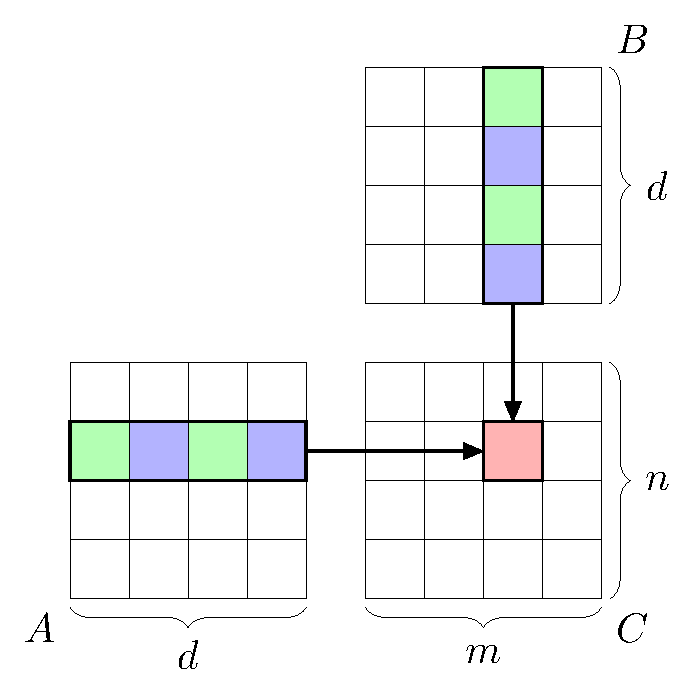
\includegraphics[width=0.5\textwidth]{HLPP/mm}
  \caption[Visalization of matrix multiplication.]%
          {Matrix multiplication $A\times B = C$.
           The red highlighted element in matrix $C$ is computed by combining the highlighted row of matrix $A$ with the highlighted column of matrix $B$.}
  \label{fig:mm}
\end{figure}


\subsubsection*{\SkelCL Implementation}
\autoref{eq:skelcl:mm} shows how matrix multiplication can be expressed using the \allpairs skeleton in \SkelCL:
\begin{align}
  \label{eq:skelcl:mm}
  mm\ A\ B &= allpairs\ f\ A\ B^T\\
  \text{where:} \qquad f\ \vec{a}\ \vec{b} &= \sum_{k=0}^d a_k \times b_k \nonumber
\end{align}
When looking back at \autoref{sec:dot}, we can see, that $f$ is actually the dot product computation, therefore, we can write:
\begin{align}
  mm\ A\ B &= allpairs\ dotProduct\ A\ B^T
  \label{eq:skelcl:mm:dot}
\end{align}
We know that we can express the dot product as a sequential composition of the \zip and \reduce skeletons.
In \autoref{section:skelcl-programming-model:specialSkeletons} we discussed a specialized implementation of the \allpairs skeleton for computations which can be expressed in this way.
Therefore, we can use the \SkelCL library to develop two implementations:
1) using the generic \allpairs skeleton; and 2) using the specialized \allpairs skeleton.

\autoref{lst:skelcl:mm:generic} shows the implementation of matrix multiplication using the generic \allpairs skeleton.
\begin{lstlisting}[%                                                             
caption={Implementation of matrix multiplication using the generic \allpairs skeleton in \SkelCL.},%
numbers=left,%
float=tb,
label={lst:skelcl:mm:generic}]
Matrix<float> mm(const Matrix<float>& A,$\label{lst:skelcl:mm:generic:CPU:start}$
                 const Matrix<float>& B) {
  skelcl::init();
  auto mm = allpairs($\label{lst:skelcl:mm:generic:CPU:stop}$
    [](const Vector<float>& a, const Vector<float>& b) {$\label{lst:skelcl:mm:generic:GPU:start}$
      float c = 0.0f;
      for (int i = 0; i < a.size(); ++i)
        c += a[i] * b[i];
      return c; });$\label{lst:skelcl:mm:generic:GPU:stop}$
  return mm(A, B); }$\label{lst:skelcl:mm:generic:CPU:call}$
\end{lstlisting}
The skeleton is customized with a lambda expression processing two vectors:
$a$ is a row vector of matrix $A$ and $b$ is a column vector of matrix $B$.
In this generic implementation the dot product computation is implemented using a \code{for} loop iterating over the vectors, multiplying elements pairwise and summing them up in the accumulation variable $c$.

\autoref{lst:skelcl:mm:special} shows the implementation of matrix multiplication using the specialized \allpairs skeleton.
\begin{lstlisting}[%                                                             
caption={Implementation of matrix multiplication using the specialized \allpairs skeleton in \SkelCL.},%
float=tb,%                                                                       
numbers=left,%
label={lst:skelcl:mm:special}]
Matrix<float> mm(const Matrix<float>& A,
                 const Matrix<float>& B) {
  skelcl::init();
  auto mult  = zipVector($\label{lst:skelcl:mm:special:zip}$
      [](float x, float y){return x*y;});$\label{lst:skelcl:mm:special:zipGPU}$
  auto sumUp = reduce($\label{lst:skelcl:mm:special:reduce}$
      [](float x, float y){return x+y;}, 0);$\label{lst:skelcl:mm:special:reduceGPU}$
  auto mm    = allpairs(sumUp, mult);
  return mm(A, B); }
\end{lstlisting}
Here the \allpairs skeleton is customized with \zip and \reduce skeletons defined in lines~\ref{lst:skelcl:mm:special:zip} and~\ref{lst:skelcl:mm:special:reduce}.
This implementation corresponds more closely to \autoref{eq:skelcl:mm:dot}:
as we express the dot product using these two skeletons (as shown in \autoref{sec:dot}).
Therefore, we reuse the definitions of \code{mult} and \code{sumUp} as used in \autoref{lst:skelcl:dot}.

\subsubsection*{Implementations used for comparison}
We compare six different implementations of matrix multiplication:
\begin{enumerate}
  \item the OpenCL implementation from~\cite{KirkHw2010} without optimizations,
  \item the optimized OpenCL implementation from~\cite{KirkHw2010} using \GPU local memory,
  \item the optimized BLAS implementation by AMD~\cite{APPML} written in OpenCL,
  \item the optimized BLAS implementation by Nvidia~\cite{cuBLAS} written in CUDA,
  \item the \SkelCL implementation in~\autoref{lst:skelcl:mm:generic} using the generic \allpairs skeleton,
  \item the \SkelCL implementation in~\autoref{lst:skelcl:mm:special} using the specialized \allpairs skeleton.
\end{enumerate}

\paragraph{1. OpenCL implementation}
The kernel of the first, unoptimized OpenCL implementation from~\cite{KirkHw2010} is shown in \autoref{lst:naive_opencl}.
\begin{lstlisting}[%                                                             
caption={[\OpenCL kernel of matrix multiplication without optimizations.]\OpenCL kernel of matrix multiplication without optimizations~\cite{KirkHw2010}.},%
float=tb,%
numbers=left,%
label={lst:naive_opencl}]
kernel void mm(global float* A, global float* B,
               global float* C, int m, int d, int n) {
  int row = get_global_id(0); int col = get_global_id(1);
  float sum = 0.0f;
  for (int k = 0; k < d; k++)
    sum += A[row * d + k] * B[k * n + col];
  C[row * n + col] = sum; }
\end{lstlisting}

\vspace{-.5em}
\paragraph{2. Optimized OpenCL implementations}
The kernel of the optimized OpenCL implementation from~\cite{KirkHw2010} using local memory is shown in \autoref{lst:local_mem_opencl}.
\begin{lstlisting}[%                                                             
caption={[\OpenCL kernel of the optimized matrix multiplication usgin local memory.]\OpenCL kernel of the optimized matrix multiplication using local memory~\cite{KirkHw2010}.},%
float=tb,%
numbers=left,%
label={lst:local_mem_opencl}]
#define T_WIDTH 16
kernel void mm(global float* A, global float* B,
               global float* C, int m, int d, int n) {
  local float Al[T_WIDTH][T_WIDTH];$\label{lst:local_mem_opencl:allocA}$
  local float Bl[T_WIDTH][T_WIDTH];$\label{lst:local_mem_opencl:allocB}$
  int row = get_global_id(0); int col = get_global_id(1);
  int l_row = get_local_id(0);  int l_col = get_local_id(1);
  float sum = 0.0f;
  for (int m = 0; m < d / T_WIDTH; ++m {$\label{lst:local_mem_opencl:loop}$
    Al[l_row][l_col] = A[row * d + (m * T_WIDTH + l_col)];$\label{lst:local_mem_opencl:loadA}$
    Bl[l_row][l_col] = B[(m * T_WIDTH + l_row) * d + col];$\label{lst:local_mem_opencl:loadB}$
    barrier(CLK_LOCAL_MEM_FENCE);$\label{lst:local_mem_opencl:barrier1}$
    for (int k = 0; k < T_WIDTH; k++)
      sum += Al[l_row][k] * Bl[k][l_col];$\label{lst:local_mem_opencl:comp}$
    barrier(CLK_LOCAL_MEM_FENCE); }$\label{lst:local_mem_opencl:barrier2}$
  C[row * n + col] = sum; }
\end{lstlisting}
Two fixed-sized arrays of local memory are allocated in lines~\ref{lst:local_mem_opencl:allocA} and~\ref{lst:local_mem_opencl:allocB}.
Matrix multiplication is carried out in the loop starting in line~\ref{lst:local_mem_opencl:loop}.
In each iteration, data is loaded into the local memory (lines~\ref{lst:local_mem_opencl:loadA} and~\ref{lst:local_mem_opencl:loadB}) before it is used in the computation in line~\ref{lst:local_mem_opencl:comp}.
Note that two synchronization barriers are required (lines~\ref{lst:local_mem_opencl:barrier1} and~\ref{lst:local_mem_opencl:barrier2}) to ensure that the data is fully loaded into the local memory and that the data is not overwritten while other work-items are still using it.

Both OpenCL implementations 1. and 2. from~\cite{KirkHw2010} are restrictive:
they are only capable of performing matrix multiplication for square matrices.

\vspace{-.5em}
\paragraph{3. BLAS implementation by AMD}
The implementation offered by AMD is called clBLAS, written in OpenCL and is part of their Accelerated Parallel Processing Math Libraries (APPML)~\cite{APPML}.

\vspace{-.5em}
\paragraph{4. BLAS implementation by NVIDIA}
The cuBLAS~\cite{cuBLAS} is implemented using CUDA and, therefore, can only be used on GPUs built by NVIDIA.

\subsubsection*{Programming effort}
\autoref{fig:mat_mult_loc} shows the comparison regarding the number of lines of code (LoCs) required for each of the six implementations.
\autoref{tab:mat_mult_loc} presents the detailed numbers.
We did not count those LoCs which are not relevant for parallelization and are similar in all six implementations, like initializing the input matrices with data and checking the result for correctness.
For every implementation, we distinguish between \CPU (host) code and \GPU (kernel) code.

In the \OpenCL implementations, the \GPU code includes the kernel definition, as shown in \autoref{lst:naive_opencl} and \autoref{lst:local_mem_opencl};
the \CPU code includes the initialization of \OpenCL, memory allocations, explicit data transfer operations, and management of the execution of the kernel.

In the BLAS implementations, the \CPU code contains the initialization of the corresponding BLAS library, memory allocations, as well as a library call for performing the matrix multiplication;
no separate definition of \GPU code is necessary, as the \GPU code is defined inside the library function calls.

For the implementation based on the generic \allpairs skeleton (\autoref{lst:skelcl:mm:generic}), we count lines~\ref{lst:skelcl:mm:generic:CPU:start}--\ref{lst:skelcl:mm:generic:CPU:stop} and~\ref{lst:skelcl:mm:generic:CPU:call} as the \CPU code, and the definition of the customizing function in lines~\ref{lst:skelcl:mm:generic:GPU:start}--\ref{lst:skelcl:mm:generic:GPU:stop} as the \GPU code.
For the implementation based on the specialized \allpairs skeleton (\autoref{lst:skelcl:mm:special}), lines~\ref{lst:skelcl:mm:special:zipGPU} and~\ref{lst:skelcl:mm:special:reduceGPU} are the \GPU code, while all other lines constitute the \CPU code.

Both skeleton-based implementations are clearly the shortest, with 10 and 9 LoCs.
The next shortest implementation is the cuBLAS implementation with 65 LoCs -- 7 times longer than the \SkelCL-based implementations.
The other three implementations using \OpenCL require even 9 times more LoCs than the \SkelCL-based implementations.

Besides their length, the \OpenCL-based implementations require the application developer to explicitly implement many low-level, error-prone tasks, like dealing with pointers and offset calculations.
Furthermore, the skeleton-based implementations are more general, as they can be used for arbitrary allpairs computations, while all \OpenCL-based implementations can compute matrix multiplication only.

\begin{figure}[tb]
  \centering
  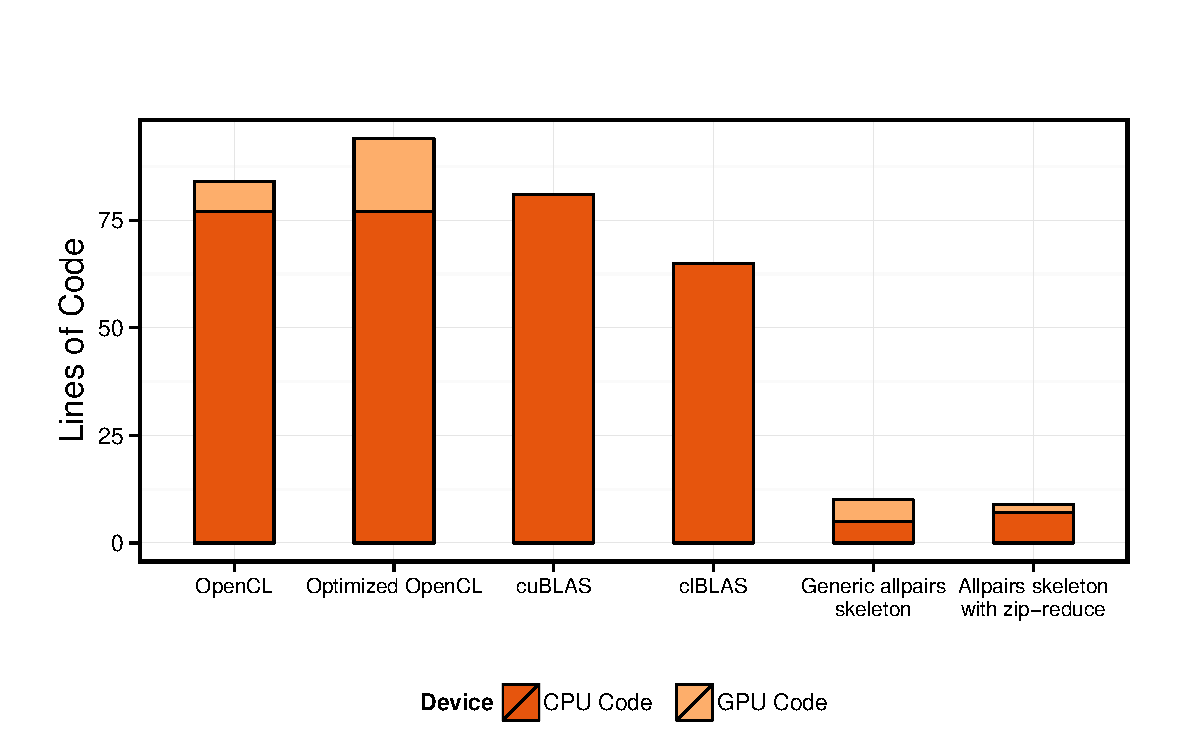
\includegraphics[width=0.9\textwidth]{HLPP/mat_mult_loc}
  \caption[Programming effort of four \OpenCL-based and two \SkelCL-based matrix multiplication implementations.]%
          {Programming effort (Lines of Code) of four \OpenCL-based vs. two \SkelCL-based implementations.}
  \label{fig:mat_mult_loc}
\end{figure}
\begin{table}[tb]
  \centering
  \begin{tabular}{lrr}
    \toprule
              & \multicolumn{2}{c}{Lines of Code} \\
    \cmidrule(r){2-3}
    Implementation & \CPU & \GPU \\
    \midrule
    \OpenCL           & 77 &  7 \\
    Optimized \OpenCL & 71 & 17 \\
    cuBLAS            & 81 & -- \\
    clBLAS            & 65 & -- \\
    Generic \allpairs  & \multirow{2}{*}{5} & \multirow{2}{*}{5}\\
    skeleton\\
    Specialized \allpairs & \multirow{2}{*}{7} & \multirow{2}{*}{2}\\
    skeleton\\
    \bottomrule
  \end{tabular}
  \caption[Lines of Code of matrix multiplication of all compared implementaitons.]%
          {Lines of Code of all compared implementations.}
  \label{tab:mat_mult_loc}
\end{table}

\subsubsection*{Performance experiments}
We performed our experiments with the six different implementations 1. -- 6. of matrix multiplication on two different computer systems with GPUs:
\begin{itemize}[leftmargin=50pt]
  \item[System A:] Our general testing system already described in~\autoref{sec:skelcl:experimental_setup}:
    an NVIDIA S1070 equipped with four Nvidia Tesla \GPUs, each with 240 streaming processors and 4 GByte memory.
  \item[System B:] An AMD Radeon HD 6990 graphics card containing two \GPUs, each with 1536 streaming processors and 1 GByte memory.
\end{itemize}

\begin{figure}[tb]
  \centering
  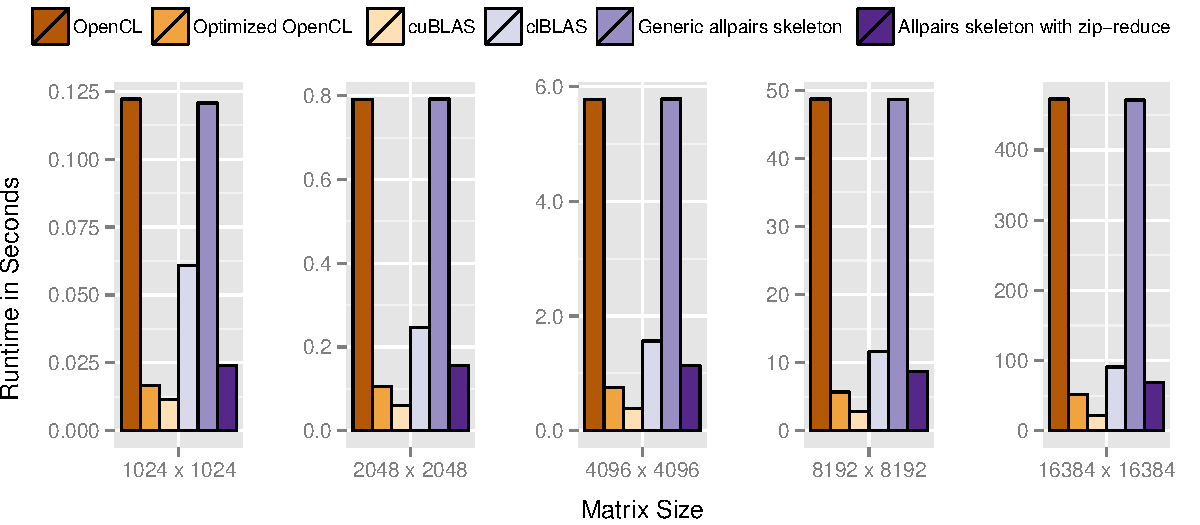
\includegraphics[width=0.9\textwidth]{HLPP/mat_mult_sizes}
  \caption[Runtime of different matrix multiplication implementations on an NVIDIA system.]%
          {Runtime of different matrix multiplication implementations on the NVIDIA system for different sizes of the matrices.}
  \label{fig:mat_mult_single}
\end{figure}
\begin{table}[tb]
  \centering
  \begin{tabular}{lrrrrr}
    \toprule
              & \multicolumn{5}{c}{Runtimes in Seconds} \\
    \cmidrule(r){2-6}
    \multirow{2}{*}{Implementation} & $1024$ & $2048$ & $4096$ & $8192$ & $16384$ \\
                                    & $\times 1024$ & $\times 2048$ & $\times 4096$ & $\times 8192$ & $\times 16384$\\
    \midrule
    \OpenCL            & 0.122 & 0.791 & 5.778 & 48.682 & 472.557 \\
    Optimized \OpenCL  & 0.017 & 0.105 & 0.752 &  5.683 &  51.337 \\
    cuBLAS             & 0.012 & 0.059 & 0.387 &  2.863 &  22.067 \\
    clBLAS             & 0.061 & 0.246 & 1.564 & 11.615 &  90.705 \\
    Generic \allpairs  & \multirow{2}{*}{0.121} & \multirow{2}{*}{0.792} & \multirow{2}{*}{5.782} & \multirow{2}{*}{48.645} & \multirow{2}{*}{471.235} \\
    skeleton\\
    Specialized \allpairs & \multirow{2}{*}{0.024} & \multirow{2}{*}{0.156} & \multirow{2}{*}{1.134} & \multirow{2}{*}{8.742} & \multirow{2}{*}{68.544} \\
    skeleton\\
    \bottomrule
  \end{tabular}
  \caption[Runtime results for all tested implementations of matrix multiplication on an NVIDIA system.]
          {Runtime results for all tested implementations on the NVIDIA system.}
  \label{tab:mat_mult_single}
\end{table}

In all our experiments, we include the time of data transfers to and from the \GPU, \ie the measured runtime consists of:
1) uploading the two input matrices to the \GPU;
2) performing the actual matrix multiplication;
3) downloading the computed result matrix.

\paragraph{System A (one \GPU)}
\autoref{fig:mat_mult_single} shows the runtime in seconds of all six implementations for different sizes of the matrices (note that for readability reasons, all charts are scaled differently).
For detailed numbers, see \autoref{tab:mat_mult_single}.

Clearly, the naive \OpenCL-based implementation and the \SkelCL-based implementation using the generic \allpairs skeleton are the slowest, because both do not use the fast \GPU local memory, in contrast to all other implementations.

The \SkelCL-based implementation using the specialized \allpairs skeleton performs between 5.0 and 6.8 times faster than the implementation using the generic allpairs skeleton, but is 33\% slower on $16384\times 16384$ matrices than the optimized \OpenCL-based implementation using local memory.
However, the latter implementation can only be used for square matrices and, therefore, it benefits from omitting many conditional statements and boundary checks.

\begin{figure}[tb]
  \centering
  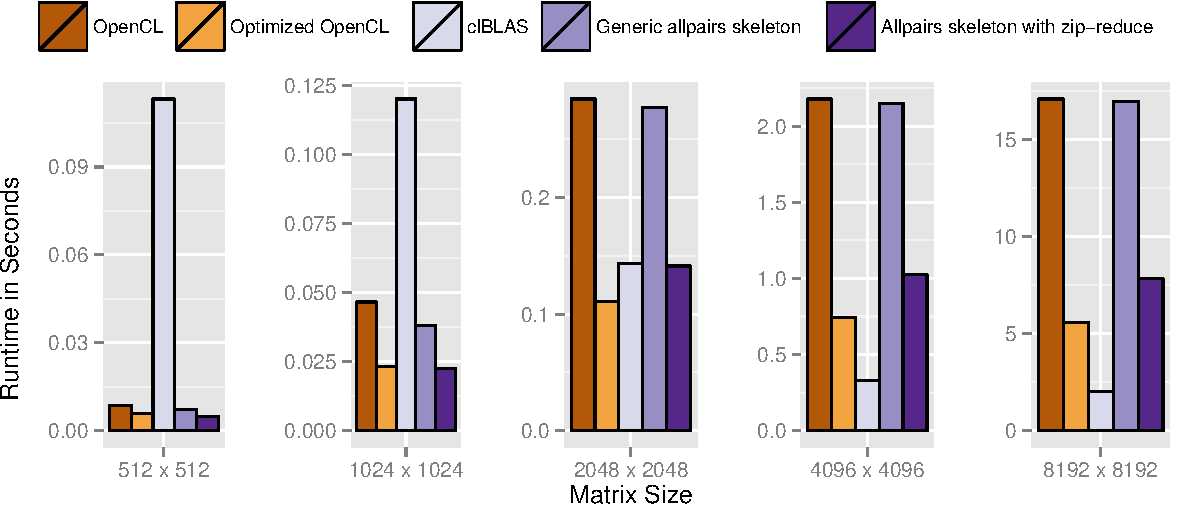
\includegraphics[width=0.9\textwidth]{HLPP/mat_mult_sizes_hd6990}
  \caption[Runtime of different matrix multiplication implementations on an AMD ststem.]%
          {Runtime of all compared implementations for a matrix multiplication on the AMD system using one \GPU.}
  \label{fig:mat_mult_single_amd}
\end{figure}
\begin{table}[b]
  \centering
  \begin{tabular}{lrrrrr}
    \toprule
              & \multicolumn{5}{c}{Runtimes in Seconds} \\
    \cmidrule(r){2-6}
    \multirow{2}{*}{Implementation} & $512$ & $1024$ & $2048$ & $4096$ & $8192$ \\
                                    & $\times 512$ & $\times 1024$ & $\times 2048$ & $\times 4096$ & $\times 8192$ \\
    \midrule
    \OpenCL            & 0.008 & 0.046 & 0.284 & 2.178 & 17.098 \\
    Optimized \OpenCL  & 0.006 & 0.023 & 0.111 & 0.743 &  5.569 \\
    clBLAS             & 0.113 & 0.120 & 0.143 & 0.329 &  2.029 \\
    Generic \allpairs  & \multirow{2}{*}{0.007} & \multirow{2}{*}{0.038} & \multirow{2}{*}{0.278} & \multirow{2}{*}{2.151} & \multirow{2}{*}{16.983} \\
    skeleton\\
    Specialized \allpairs & \multirow{2}{*}{0.005} & \multirow{2}{*}{0.023} & \multirow{2}{*}{0.141} & \multirow{2}{*}{1.025} & \multirow{2}{*}{7.842} \\
    skeleton\\
    \bottomrule
  \end{tabular}
  \caption[Runtime results for all tested implementations of matrix multiplication on an AMD system.]%
          {Runtime results for all tested implementations of matrix multiplication on the AMD system.}
  \label{tab:mat_mult_single_amd}
\end{table}

Not surprisingly, cuBLAS by Nvidia is the fastest of all implementations, as it is highly tuned specifically for Nvidia \GPUs using CUDA.
The clBLAS implementation by AMD using \OpenCL performs not as well:
presumably, it is optimized for AMD \GPUs and performs poorly on other hardware.
Our optimized \allpairs skeleton implementation outperforms the clBLAS implementation for all matrix sizes tested.

\paragraph{System B (one \GPU)}
\autoref{fig:mat_mult_single_amd} shows the measured runtime in seconds for five of the six implementations for different sizes of the matrices.
Detailed numbers can be found in \autoref{tab:mat_mult_single_amd}.
We could not use the Nvidia-specific cuBLAS implementation as it does not work on the AMD \GPU.

For bigger matrices, the slowest implementations are, again, the unoptimized \OpenCL implementation and the implementation using the generic \allpairs skeleton.

The optimized \OpenCL implementation and the specialized \allpairs skeleton perform similarly.
For matrices of size $8192\times 8192$, the optimized \OpenCL implementation is about 30\% faster.

The clBLAS implementation performs very poorly for small matrices, but is clearly the fastest implementation for bigger matrices.
Similar to the cuBLAS implementation on the Nvidia hardware, it is not surprising that the implementation by AMD performs very well on their own hardware.


\begin{figure}[tb]
  \centering
  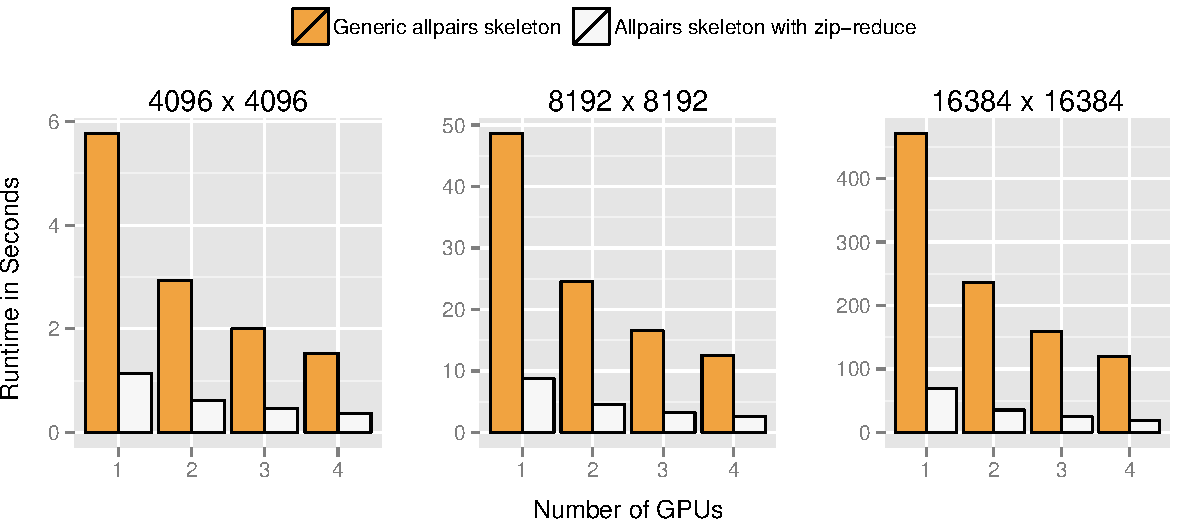
\includegraphics[width=0.9\textwidth]{HLPP/mat_mult_devices}
  \caption[Runtime of the \allpairs based matrix multiplication implementations using multiple \GPUs.]%
          {Runtime of the \allpairs based implementations using multiple \GPUs.}
  \label{fig:mat_mult_devices}
\end{figure}
\begin{table}[tb]
  \centering
  \begin{tabular}{llrrrcr}
    \toprule
              & & \multicolumn{3}{c}{Runtimes in Seconds} & & GFlops\\
    \cmidrule(r){3-5}
    \cmidrule(r){7-7}
    \multirow{2}{*}{Implementation}
     & Number    & $4096$ & $8192$ & $16384$ & & $16384$\\
     & of \GPUs   & $\times 4096$ & $\times 8192$ & $ \times 16384$ & & $ \times 16384$\\
    \midrule
    \multirow{4}{*}{\parbox[t]{2.3cm}{Generic \allpairs\\ skeleton}}
     & 1 \GPU  & 5.772 & 48.645 & 471.328 &&  18.72\\
     & 2 \GPUs & 2.940 & 24.495 & 236.628 &&  37.43\\
     & 3 \GPUs & 2.000 & 16.532 & 158.611 &&  56.17\\
     & 4 \GPUs & 1.527 & 12.540 & 119.786 &&  74.90\\[.5em]
    \multirow{4}{*}{\parbox[t]{2.3cm}{Specialized \allpairs\\ skeleton}}
     & 1 \GPU  & 1.137 &  8.740 &  68.573 && 130.93\\
     & 2 \GPUs & 0.613 &  4.588 &  35.294 && 262.18\\
     & 3 \GPUs & 0.461 &  3.254 &  24.447 && 392.87\\
     & 4 \GPUs & 0.368 &  2.602 &  19.198 && 523.91\\
    \bottomrule
  \end{tabular}
  \caption{Runtime of the allpairs based implementations of matrix multiplication using multiple \GPUs.
    For the matrices of size $16384\times 16384$ the results are also shown in GFlops.}
  \label{tab:mat_mult_devices}
\end{table}

\paragraph{System A (multiple \GPUs)}
\autoref{fig:mat_mult_devices} shows the runtime behavior for both \allpairs skeleton-based implementations when using up to four \GPUs of our multi-\GPU system.
The other four implementations are not able to handle multiple \GPUs and would have to be specially rewritten for such systems.
The newer version of Nvidia's cuBLAS implementation~\cite{} supports the execution on multiple \GPUs as well.
We observe a good scalability for both of our skeleton-based implementations, achieving speedups between 3.09 and 3.93 when using four \GPUs.
Detailed numbers can be found in \autoref{tab:mat_mult_devices}.
For the matrices of size $16384\times 16384$, performance is also provided in GFlops;
to compute this value we excluded the data-transfer time (as usually done in related work) for a better comparison.

\FloatBarrier




\section{Image Processing Applications}
\label{sec:imageProcessing}
Many image processing applications are inherently parallel as they often independently process the pixels of an image.
Common examples range from simple thresholding over noise reduction applications to techniques used in edge detection and pattern recognition~\cite{Umbaugh1997}.
In this section we will study three application examples from image processing and how they can be implemented using \SkelCL.

We start by looking at the Gaussian blur application which reduces noise in images and is often used as a preprocessing step in more complex algorithms.
We will then discuss two algorithms used for edge detection in images:
first, the Sobel edge detection application will be presented before, finally, the more complex Canny edge detection algorithm will be discussed.

All these three applications can be expressed using the \stencil skeleton but have different characteristics.
The Gaussian blur applies a single stencil computation, possibly iterated multiple times, for reducing the noise in images.
The Sobel edge detection applies a stencil computation once to detect edges in images.
The more advanced Canny edge detection algorithm consists of a sequence of stencil operations which are applied to obtain the final result.
For each application, we compare the performance of our two implementations of the \stencil skeletons: \code{MapOverlap} and \code{Stencil} with native OpenCL implementations using an input image of size $4096 \times 3072$.










\subsection{Gaussian blur}
\label{sec:gauss}
The Gaussian blur is a standard algorithm used in image processing~\cite{Umbaugh1997}.
One common application is reduction of image noise as shown in \autoref{fig:lena:noise}.
%
\begin{figure}[tb]
  \centering
  \begin{subfigure}[t]{.45\textwidth}
    
\includegraphics[width=\textwidth]{lenaNoise}
    \caption{Image with noise.}
    \label{fig:lena:noise:yes}
  \end{subfigure}
  \hfill
  \begin{subfigure}[t]{.45\textwidth}
    
\includegraphics[width=\textwidth]{lenaNoNoise}
    \caption{Image after applying the Gaussian blur.}
    \label{fig:lena:noise:no}
  \end{subfigure}
  \caption{Effect of applying the Gaussian blur to an noised image.}
  \label{fig:lena:noise}
\end{figure}
%
The image on the left has some noise as it is typically produced by halftone printing used to print newspapers.
The Gaussian blur has been applied to reduce the noise and produce the image on the right.

The Gaussian blur computes the color of every pixel using a weighted average of the neighboring pixel color values.
Using \SkelCL this application can easily be expressed using the \stencil skeleton.

\subsubsection*{\SkelCL Implementation}
\autoref{eq:gauss} shows the implementation in \SkelCL using the \stencil skeleton.
\begin{align}
  \label{eq:gauss}
  gauss&\ M = stencil\ f\ 1\ \overline{0}\ M \qquad\text{where:}\\
  &
  \begin{array}{ll}%
  f\ &\left[\begin{array}{lll}%
      \hspace{-.5em} M_{i-1,j-1}& \hspace{-.5em} M_{i-1,j} & \hspace{-.5em}M_{i-1,j+1}\vspace{-.25em}\\%
      \hspace{-.5em} M_{i,j-1}& \hspace{-.5em} M_{i,j} & \hspace{-.5em}M_{i,j+1}\vspace{-.25em}\\%
      \hspace{-.5em} M_{i+1,j-1}& \hspace{-.5em} M_{i+1,j} & \hspace{-.5em}M_{i+1,j+1}
    \end{array}\right]  = \\[2em]
          &\qquad \displaystyle\frac{\displaystyle\sum_{k=-1}^{1} \sum_{l=-1}^{1} (G\ k\ l)\cdot M_{i+k, j+k}}{9}
  \end{array} \nonumber\\[1em]
  &G\ x\ y = \frac{1}{2\pi \sigma^{2}} e^{-\frac{x^2 + y^2}{2\sigma^2}} \nonumber\\
  \text{and } \overline{0} \text{ is th}&\text{e constant function always returning 0.}\nonumber
\end{align}
$G$ is the two dimensional Gaussian function used in the customizing function $f$ to weight the neighboring values $M_{i,j}$.
The values gained from applying $G$ can be precomputed, as $G$ is only evaluated with values in the interval $[-1, 1]$ for $x$ and $y$.


\autoref{lst:skelcl:gauss} shows the implementation in the \SkelCL library of the Gaussian blur using the \code{MapOverlap} implementation of the \stencil skeleton.
Here the immediate neighboring pixels are access (lines~\ref{lst:skelcl:gauss:start}--\ref{lst:skelcl:gauss:end}) and used to compute a weighted value for each pixel.
The function performing the weighted sum is omitted here.
It is also possible to extend the \emph{range} of the Gaussian blur and include more neighboring pixel values in the computation.

\begin{lstlisting}[%                                                             
caption={Implementation of the Gaussian blur in \SkelCL using the \code{MapOverlap} implementation of the \stencil skeleton.},%
numbers=left,%
float=tb,
label={lst:skelcl:gauss}]
Matrix<char> gaussianBlur(const Matrix<char>& image) {
  auto gauss = mapOverlap(
    [](Neighborhood<char>& in) {
      char ul = in[{-1, -1}];$\label{lst:skelcl:gauss:start}$
      ...
      char lr = in[{+1, +1}];$\label{lst:skelcl:gauss:end}$
      return computeGaussianBlur(ul, ..., lr); },
    1, BorderHandling::NEUTRAL(0));
  return gauss(image); }
\end{lstlisting}

\subsubsection*{Programming effort}

\begin{figure}[tbp]
	\centering
	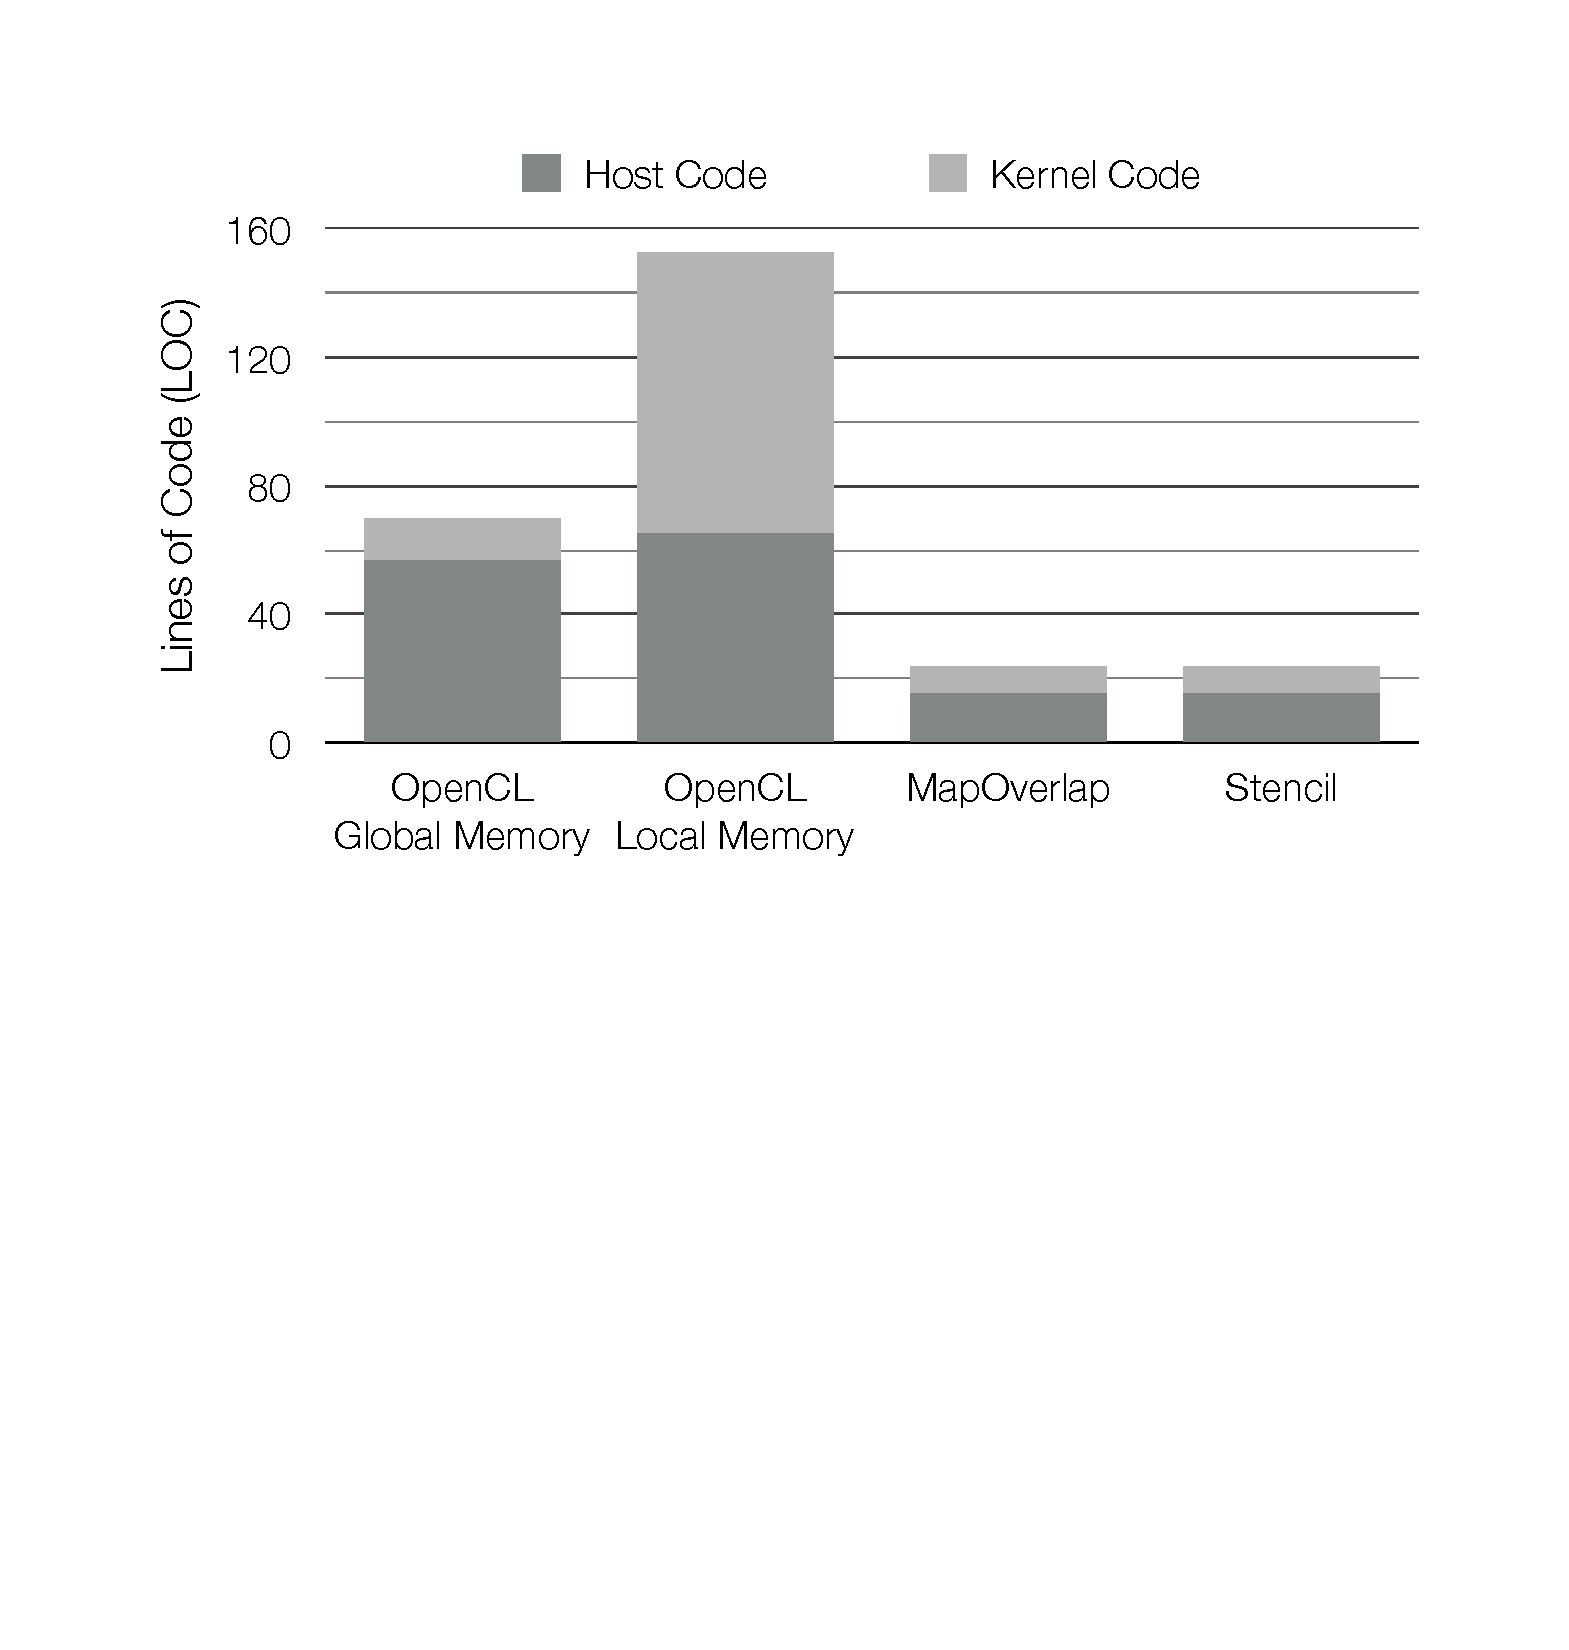
\includegraphics[width=\columnwidth]{HiStencils/LOC.pdf}
	\caption{Lines of code of the Gaussian blur using a na{\"i}ve OpenCL implementation with global memory, an optimized OpenCL version using local memory and \SkelCL's \code{MapOverlap} and \code{Stencil} implementations of the \stencil skeleton.}
	\label{fig:gaussLOCs}
\end{figure} 

\autoref{fig:gaussLOCs} shows the program sizes (in lines of code) for the four implementations. 
The application developer needs $57$ lines of OpenCL host code and 13 LOCs for performing a Gaussian blur with global memory. 
When using local memory, some more arguments are passed to the kernel, increasing the host-LOCs to $65$, while the LOCs for the kernel function, which copies all necessary elements for a work-group's calculation into local memory, requires $88$ LOCs with explicit out-of-bounds handling and complex index calculations.
\code{MapOverlap} and \code{Stencil} are similar to use and both require only $15$ LOCs host code and $9$ LOCs kernel code to perform a Gaussian blur. 
The support for multi-\GPU systems is implicitly given when using \SkelCL's skeletons, such that the kernel remains the same as for one-\GPU systems.
This is an important advantage of \SkelCL over the \OpenCL implementations of the Gaussian blur which are single-\GPU only, and they require additional LOCs when fitting to multi-\GPU environments.

The implementations using MapOverlap and Stencil are only $5-10\%$ slower than an optimized OpenCL implementation of the Gaussian blur while being much shorter than the OpenCL version.

\subsubsection*{Performance experiments}

\begin{figure}[tbp]
	\centering
	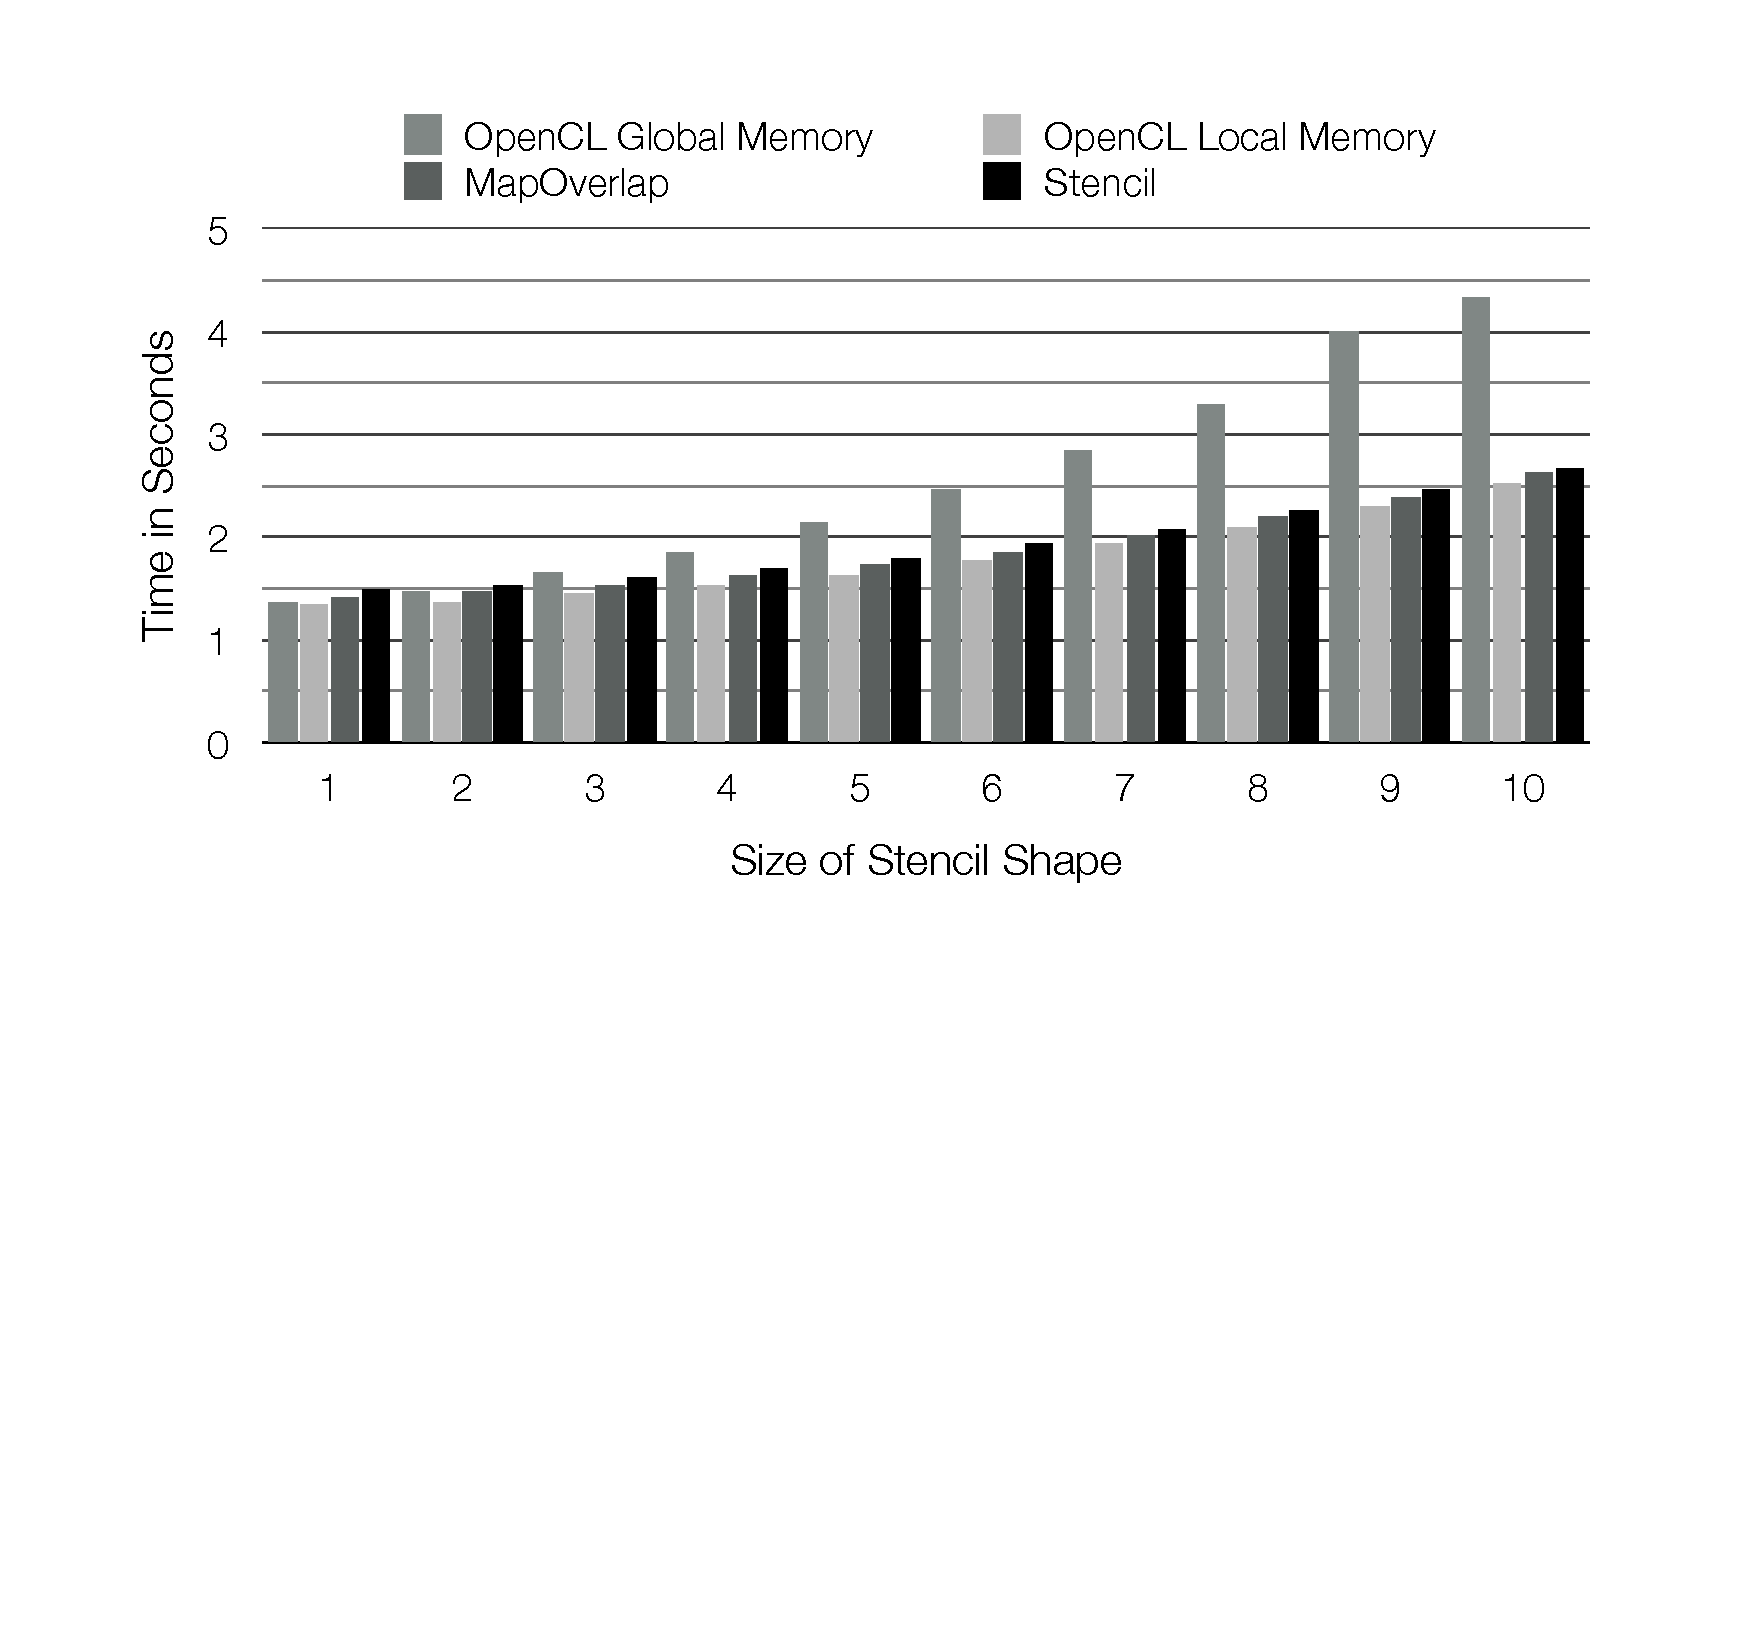
\includegraphics[width=\columnwidth]{HiStencils/GaussOpenCL.pdf}
	\caption{Runtime of the Gaussian blur using a na{\"i}ve OpenCL implementation with global memory, an OpenCL version using local memory and SkelCL's MapOverlap and Stencil skeletons.}
	\label{fig:gaussAbs}
\end{figure} 

\autoref{fig:gaussAbs} shows the total runtime of the Gaussian blur using:
1) a na{\"i}ve OpenCL implementation using global memory,
2) an optimized OpenCL version using local memory, and
3) the \code{MapOverlap} implementation, and
4) the \code{Stencil} implementation of the \stencil skeletons for different sizes of stencil shape, correspondingly.
We observe that on larger stencil shape sizes, \code{MapOverlap} and \code{Stencil} outperform the na{\"i}ve OpenCL implementation by $65\%$ and $62\%$, respectively.
The optimized OpenCL version, which copies all necessary elements into local memory prior to calculation, is $5\%$ faster than \code{MapOverlap} and $10\%$ faster than \code{Stencil} for small stencil shapes.
When increasing the stencil shape size, this disadvantage is reduced to $3\%$ for \code{MapOverlap} and $5\%$ for \code{Stencil} with stencil shape's extent of $10$ in each direction.

The \code{Stencil} implementation is slower for small stencil shapes than the \code{MapOverlap} implementation, up to $32\%$ slower for an stencil shape size of $1$.
This is due to the increased branching required in the \code{Stencil} implementation, as discussed in more detail in \autoref{sec:skelcl:stencil}.
However, this disadvantage is reduced to $4.2\%$ for an stencil shape size of $5$ and becoming negligible for bigger stencil shape sizes.
% Due to the increased branching in Stencil's kernel function, one might expect a worse runtime for the Stencil skeleton. 
As the ratio of copying into local memory decreases in comparison to the number of calculations when enlarging the stencil shape's extents, the \code{Stencil} implementation kernel function's runtime converges to the \code{MapOverlap} implementation's.
The \code{Stencil} implementation's disadvantage is also due to its ability to manage multiple stencil shapes and explicitly support the use of iterations.
While both features are not used in this use case, they incur some overhead for the implementation as compared to the \code{MapOverlap} implementation for simple stencil computations.


\autoref{fig:GaussMult} shows the speedup achieved on the Gaussian blur using the \code{Stencil} implementation on up to four devices.
The higher the computational complexity for increasing size of stencil shape, the better the overhead is hidden, leading to a maximum speedup of $1.90$ for two devices, $2.66$ for three devices, and $3.34$ for four devices.
\begin{figure}
	\centering
	\includegraphics[width=.85\columnwidth]{HiStencils/SpeedupGauss.pdf}
	\caption{Speedup on up to four \GPUs.}
	\label{fig:GaussMult}
\end{figure} 










\subsection{Sobel edge detection}
\label{sec:sobel}
The Sobel edge detection produces an output image in which the detected edges in the input image are marked in white and plain areas are shown in black.
The effect is shown in \autoref{fig:sobel:lena}, where the original image is shown on the left and the output of Sobel edge detection applied to it on the right.

\begin{figure}[tb]
  \centering
  \begin{subfigure}[t]{.45\textwidth}
    \includegraphics[width=\textwidth]{Paraphrase/lena.png}
    \caption{Original image.}
    \label{fig:lena:orig}
  \end{subfigure}
  \hfill
  \begin{subfigure}[t]{.45\textwidth}
    \includegraphics[width=\textwidth]{Paraphrase/sobel_filtered-lena.png}
    \caption{Image after Sobel edge detection.}
    \label{fig:lena:sobel}
  \end{subfigure}
  \caption{The famous Lena image~\cite{Lena} often used as an example in image processing before (left) and after (right) applying Sobel edge detection.}
  \label{fig:sobel:lena}
\end{figure}

\begin{lstlisting}[%
caption={Sequential implementation of the Sobel edge detection.},%
float=tb,
label={lst:sobel:seq}]
for (i = 0; i < width; ++i)
  for (j = 0; j < height; ++j)
    h = -1*img[i-1][j-1] +1*img[i+1][j-1]
        -2*img[i-1][j  ] +2*img[i+1][j  ]
        -1*img[i-1][j+1] +1*img[i+1][j+1];
    v = ...;
    out_img[i][j] = sqrt(h*h + v*v);
\end{lstlisting}
\bigskip

\autoref{lst:sobel:seq} shows the algorithm of the Sobel edge detection in pseudo-code, with omitted boundary checks for brevity.
In this sequential version, for computing an output value \code{out\_img[i][j]} the input value \code{img[i][j]} and the direct neighboring elements are needed.
Therefore, the \stencil skeleton is a perfect fit for implementing the Sobel edge detection.

\subsubsection*{\SkelCL Implementation}
\autoref{eq:sobel} shows the implementation of the Sobel edge detection in \SkelCL.
\begin{align}
  \label{eq:sobel}
  sobel\ M& = stencil\ f\ 1\ \overline{0}\ M \qquad\text{where:}\\
  f\ &\left[\begin{array}{lll}%
      \hspace{-.5em} M_{i-1,j-1}& \hspace{-.5em} M_{i-1,j} & \hspace{-.5em}M_{i-1,j+1}\vspace{-.25em}\\%
      \hspace{-.5em} M_{i,j-1}& \hspace{-.5em} M_{i,j} & \hspace{-.5em}M_{i,j+1}\vspace{-.25em}\\%
      \hspace{-.5em} M_{i+1,j-1}& \hspace{-.5em} M_{i+1,j} & \hspace{-.5em}M_{i+1,j+1}
    \end{array}\right] = \displaystyle\sqrt{ h^2 + v^2 }\nonumber\\
  h & = \sum_{k=0}^2 \sum_{l=0}^2 Gx_{k, l}\cdot M_{i+k-1,j+k-1}\nonumber\\
  v & = \sum_{k=0}^2 \sum_{l=0}^2 Gy_{k, l}\cdot M_{i+k-1,j+k-1}\nonumber\\
  Gx& = \left[\begin{array}{ccc}%
      -1&0&+1\\
      -2&0&+2\\
      -1&0&+1
    \end{array}\right]
  Gy = \left[\begin{array}{ccc}%
      -1&-2&-1\\
      0&0&0\\
      +1&+2&+1
    \end{array}\right] \nonumber\\
  \text{and } \overline{0} \text{ is th}&\text{e constant function always returning 0.}\nonumber
\end{align}
The formula resembles the sequential implementation shown in \autoref{lst:sobel:seq} where the final result is computed as the square root of the sum of two squared terms $h$ and $v$.
These are computed as weighted sums of the neighboring values $M_{i,j}$.
The weights are given by the two matrices $Gx$ and $Gy$.

\autoref{lst:sobel:skelcl} shows the \SkelCL implementation using the \code{MapOverlap} implementation of the \stencil skeleton.
%
\begin{lstlisting}[%
caption={\SkelCL implementation of the Sobel edge detection.},%
numbers=left,
float=tb,
label={lst:sobel:skelcl}]
Matrix<char> sobelEdge(const Matrix<char>& image) {
  auto sobel = mapOverlap(
    [](Neighborhood<char>& in) {
      short h = -1*in[{-1,-1}] +1*in[{+1,-1}]
                -2*in[{-1, 0}] +2*in[{+1, 0}]
                -1*in[{-1,+1}] +1*in[{+1,+1}];
      short v = ...;
      return sqrt(h*h + v*v); },
    1, BorderHandling::NEUTRAL(0));
  return soble(img); }
\end{lstlisting}
%
The implementation is straightforward and very similar to the formula in \autoref{eq:sobel} and the sequential version in \autoref{lst:sobel:seq}.

\subsubsection*{Programming effort}

\begin{lstlisting}[%
caption={Additional boundary checks and index calculations for Sobel algorithm, necessary in the standard OpenCL implementation.},%
float=tb,
numbers=left,
label={lst:sobel:opencl}]
kernel void sobel_kernel( global const uchar* img,
                          global       uchar* out_img) {
 uint i = get_global_id(0);   uint j = get_global_id(1);
 uint w = get_global_size(0); uint h = get_global_size(1);
 // perform boundary checks
 if(i >= 1 && i < (w-1) && j >= 1 && j < (h-1)) {
  char ul = img[((j-1)*w)+(i-1)];
  char um = img[((j-1)*w)+(i+0)];
  char ur = img[((j-1)*w)+(i+1)];
  // ... 5 more
  char lr = img[((j+1)*w)+(i+1)];

  out_img[j * w + i] = computeSobel(ul, um, ur, ..., lr); }}
\end{lstlisting}

\autoref{lst:sobel:opencl} shows a part of the rather simple \OpenCL implementation for Sobel edge detection provided by AMD as an example for their software development kit~\cite{AMDSDK}.
The actual computation is performed inside the \texttt{computeSobel} function, which is omitted in the listing, since it is quite similar to the sequential version in \autoref{lst:sobel:seq}.
The listing shows that extra low-level code is necessary to deal with technical details, like boundary checks and index calculations, which are arguably complex and error-prone.

We also compare against a more optimized \OpenCL implementation by Nvidia which makes use of the fast local \GPU memory.

The \SkelCL implementation is significantly shorter than the cumbersome \OpenCL implementations.
The \SkelCL program only comprises the few lines of code shown in \autoref{lst:sobel:skelcl}.
The AMD implementations requires 37 lines of code for its kernel implementation and the more optimized Nvidia implementation requires even 208 lines of code.
Both versions require additional lines of code for the host program which manages the execution of the \OpenCL kernel.
No index calculations or boundary checks are necessary in the \SkelCL version whereas they are crucial for a correct implementation in \OpenCL.

\subsubsection*{Performance experiments}

\begin{figure}[tbp]
  \vspace{.5em}
  \centering
  \includegraphics[height=4.5cm]{PaCT/lena.pdf}
  \caption{Performance results for Sobel edge detection}
  \label{fig:sobel:measurements}
\end{figure}
\autoref{fig:sobel:measurements} shows the runtime of two \OpenCL versions (from the AMD and Nvidia SDKs) vs. the \SkelCL version with the \stencil skeleton presented in \autoref{lst:sobel:skelcl}.
Here only the kernel runtimes are shown, as the data transfer times are equal for all versions.
We used the popular Lena image~\cite{Lena} with a size of $512\times 512$ pixel.
The AMD version is clearly slower then the two other implementations, because it does not use the fast local memory which the Nvidia implementation and the \code{MapOverlap} implementation of the \stencil skeleton of \SkelCL do.
\SkelCL completely hides the memory management details inside its implementation from the application developer.
The Nvidia and \SkelCL implementations perform similar.
In this particular example, \SkelCL even slightly outperforms the implementation by Nvidia.










\subsection{Canny Edge Detection}
The Canny edge detection algorithm is a more complex algorithm to detect edges in images than the Sobel edge detection presented in the previous section.
For the sake of simplicity we consider a slightly simplified version, which applies the following stencil operations in a sequence:
1), a noise reduction operation is applied, \eg, a Gaussian blur;
2), an edge detection operator like the Sobel edge detection is applied;
3), the so-called non-maximum suppression is performed, where all pixels in the image are colored black except pixels being a local maximum;
4), a threshold operation is applied to produce the final result.
A more complex version of the algorithm performs the edge tracking by hysteresis, as an additional step.
This results in detecting some weaker edges, but even without this additional step the algorithm usually achieves good results.


\subsubsection*{\SkelCL Implementation}
In \SkelCL, each single step of the Canny algorithm can be expressed using the \stencil skeleton.
The last step, the threshold operation, does not need access to neighboring elements, as the user threshold function only checks the value of the current pixel.
Therefore, this step can be expressed using \SkelCL's simpler \map skeleton.
In the \SkelCL library the \code{Stencil} skeleton's implementation automatically uses the simpler \map skeleton's implementation when the user specifies a stencil shape which extents are $0$ in all directions.

\begin{lstlisting}[%
  caption={Structure of the Canny algorithm as implemented with a sequence of skeletons.},%
  float=tbp,%
  label={lst:skelcl:canny}]
Matrix<char> sobelEdge(const Matrix<char>& image) {
  auto gauss     = stencil(...);$\label{lst:skelcl:canny:step1}$
  auto sobel     = stencil(...);
  auto nms       = stencil(...);
  auto threshold = stencil(...);$\label{lst:skelcl:canny:stepN}$
  StencilSequence<Pixel(Pixel)>
      canny(gauss, sobel, nms, threshold);$\label{lst:skelcl:canny:combine}$
  return canny(image); }$\label{lst:skelcl:canny:call}$
\end{lstlisting}

To implement the Canny algorithm in SkelCL, the single steps can be combined as shown in \autoref{lst:skelcl:canny}.
The individual steps are defined in lines~\ref{lst:skelcl:canny:step1}--\ref{lst:skelcl:canny:stepN} and then combined to a sequence of stencils in line~\ref{lst:skelcl:canny:combine}.
During execution (line~\ref{lst:skelcl:canny:call}), the stencil operations are performed in the order which is specified when creating the \emph{StencilSequence} object.

\subsubsection*{Programming effort}
\todo{...}

\subsubsection*{Performance experiments}

\begin{figure}[tbp]
	\centering
	\includegraphics[width=.9\columnwidth]{HiStencils/Canny.pdf}
	\caption{Runtime of the Canny edge detection algorithm comparing the \code{MapOverlap} and \code{Stencil} skeleton implementations.}
	\label{fig:canny}
\end{figure} 

\autoref{fig:canny} shows the absolute runtime of the Canny algorithm. 
As the \code{MapOverlap} implementation appends padding elements to the matrix, the matrix has to be downloaded, resized and uploaded again to the \GPU between each step of the sequence.
This additional work to an increased time for data transfers. 
The Gaussian blur with a stencil shape extent of $2$, as well as the Sobel edge detection and the non-maximum suppression with a stencil shape of $1$, are $2.1$ to $2.2$ times faster when using \code{MapOverlap}. 
However, the threshold operation, which is expressed as the \map skeleton in the Stencil sequence, is $6.8$ times faster than \code{MapOverlap}'s threshold operation.
Overall, when performing sequences of stencil operations, the \code{Stencil} implementation reduces the number of copy operations and, therefore, leads to a better overall performance.
When performing the Canny algorithm, the \code{Stencil} implementation outperforms the \code{MapOverlap} implementation by $21\%$.



\section{Medical Imaging}
\label{section:medical-imaging}
At the beginning of \autoref{chapter:skelcl} we used the LM OSEM medical imaging application as our motivational example and application study to identify requirements for a high-level programming model.
In this section we will now study how we can express the LM OSEM application using algorithmic skeletons and how the parallel container data types and \SkelCL's redistribution feature simplify the programming of multi-GPU systems.
We will start by briefly reintroducing the application and its sequential implementation before moving to the parallel implementation using first traditional \OpenCL and then \SkelCL for comparison.
A particular focus of this section will be on multi-GPU systems and how \SkelCL radically simplifies their programming.

\subsubsection*{The LM OSEM Algorithm}
\emph{List-Mode Ordered Subset Expectation Maximization} (LM OSEM)~\cite{ReaderErFlOt1998, SchellmannGoMeKoScWuBu2009} is a time-intensive, production-quality algorithm for medical image reconstruction.
LM OSEM takes a set of events from a PET scanner and splits them into $s$ equally sized subsets.
Then, for each subset $S_l, l \in {0, \ldots, s-1}$, the following computation is performed:
\begin{equation}
 f_{l+1}=f_{l}c_{l};\quad
 c_{l}=\dfrac{1}{A_N^T \textbf{1}}
\sum_{i \in S_{l}} (A_i)^T \dfrac{1}{A_{i} f_{l}}.
\label{eq:lm_osem2}
\end{equation}
Here $f$ is the 3D reconstruction image which is refined over time.
$A$ is a matrix where element $a_{ik}$ of row $A_i$ represents the length of intersection of the line between two PET detectors for a measured event $i$ with voxel $k$ of the reconstruction image.
The factor in front of the sum can be precomputed and is, therefore, omitted from here on.

\paragraph{Sequential implementation}
\autoref{lst:lmosem:seq_code:2} shows the sequential code for LM OSEM as already presented in \autoref{section:opencl-example}.
%
\begin{figure}
\begin{lstlisting}[
  caption={[Sequential code for LM OSEM.]Sequential code for LM OSEM comprises one outer loop with two nested inner loops.},
  label={lst:lmosem:seq_code:2}]
for (int l = 0; l < subsets; l++) {$\label{lst:lmosem:seq_core:2:loop}$
  // read subset

  // step 1: compute error image $c_l$
  for (int i = 0; i < subset_size; i++) { $\label{lst:lmosem:seq_code:2:step1:begin}$
    // compute $A_i$
    // compute local error
    // add local error to $c_l$
  } $\label{lst:lmosem:seq_code:step1:end}$

  // step 2: update reconstruction image $f$
  for (int k = 0 ; k < image_size; k++) { $\label{lst:lmosem:seq_code:2:step2:begin}$
    if (c_l[k] > 0.0) { f[k] = f[k] * c_l[k]; }
  } $\label{lst:lmosem:seq_code:2:step2:end}$
}
\end{lstlisting}
\end{figure}
%
The sequential LM OSEM is an iterative algorithm refining the reconstruction image $f$ over time, at each iteration two major steps are performed:
\begin{itemize}
  \item[] \emph{Step 1:} the error image $c_l$ is computed by performing three sub-steps: 1) computation of the row $A_i$; 2) computing the local error for row $A_i$; 3) adding the local error to $c_l$;
  \item[] \emph{Step 2:} update the reconstruction image $f$ using the error image $c_l$ computed in Step 1.
\end{itemize}

\paragraph{Parallelization strategy}
For parallelization two possible decomposition strategies can be considered for the LM OSEM algorithm as initially suggested in~\cite{JonesJoKeNeReLeByBaMiCa2002}: Projection Space Decomposition (PSD) and Image Space Decomposition (ISD).

In PSD, the subsets $S_l$ are split into sub-subsets that are processed simultaneously while all processing units access a common reconstruction image $f$ and error image $c$.
Using this approach, we are able to parallelize \emph{Step~1} of the algorithm, but \emph{Step~2} is performed by a single processing unit.
On a multi-\GPU system, we have to copy the reconstruction image to all \GPUs before each iteration, and we have to merge all \GPUs' error images computed in \emph{Step~1} before proceeding with \emph{Step~2}.
While both steps are easy to implement, \emph{Step~2} does not efficiently use the available processing units.

In ISD, the reconstruction image $f$ is partitioned, such that each processing unit processes the whole subset $S_l$ with respect to a single part of the reconstruction image $f$.
Thus we are able to parallelize both steps of LM OSEM, but each processing unit still accesses the whole reconstruction image $f$ in order to compute the error value for each path before merging it with the error image $c$.
On a multi-\GPU system, the whole subset $S_l$ has to be copied to each \GPU in \emph{Step~1}.
ISD requires large amounts of memory (up to several GB in practically relevant cases) to save all paths computed in \emph{Step~1}.
Summarizing, it is hard to implement \emph{Step~1} on the \GPU, while \emph{Step~2} can be parallelized easily.

Therefore, we use a hybrid strategy for implementing LM OSEM:
\emph{Step~1} is parallelized using the PSD approach, while we use ISD for \emph{Step~2}.
This results in the sequence of five phases shown in \autoref{fig:lmosem:em_distribution2}:
\begin{enumerate}
\item \emph{Upload:} the subset ($S$) is divided into sub-subsets (one per \GPU).
      One sub-subset and the reconstruction image ($f$) are uploaded to each \GPU;
\item \emph{Step 1:} each \GPU computes the local error image ($c_l$) for its sub-subset;
\item \emph{Redistribution:} the local error images that are distributed on all \GPUs are downloaded and combined into a single error image on the host by performing element-wise addition.
      Afterwards, the combined error image and reconstruction image are partitioned, in order to switch the parallelization strategy from PSD to ISD.
      The corresponding parts of both images are distributed to the \GPUs again;
\item \emph{Step 2:} each \GPU updates its part of the reconstruction image;
\item \emph{Download:} finally, all parts of the reconstruction image are downloaded from the \GPUs to the host and merged into a single reconstruction image.
\end{enumerate}

\begin{figure}
  \centering
  \includegraphics[width=0.6\textwidth]{ICCS/em_distribution}
  \caption{Parallelization schema of the LM OSEM algorithm.}
  \label{fig:lmosem:em_distribution2}
\end{figure}


\subsubsection*{\SkelCL Implementation}

The \SkelCL program in \autoref{lst:em_skelcl} reflects the described five phases in a concise, high-level manner, as shown by the corresponding comments.
The subset \code{s}, the error image \code{cl}, and the reconstruction image \code{f} are declared as \SkelCL vectors which enables an easy and automatic data transfer between \GPUs.
As data transfers are performed implicitly by \SkelCL, the upload phase is implemented by simply setting vector distributions (lines~\ref{lst:em:skelcl:upload:start}--\ref{lst:em:skelcl:upload:end}), while the download phase is performed implicitly when the \SkelCL containers are accessed or redistributed.
\begin{lstlisting}[%
  caption={SkelCL code of the LM OSEM algorithm},%
  numbers=left,%
float,%
label={lst:em_skelcl}]
auto computeCl = mapVector(
  [](Event e, const Vector<float>& f, Vector<float>& cl) {
    Path Ai = computeAi(e);$\label{lst:em:skelcl:computeAi}$
    float c = computeLocalError(f, Ai);
    addLocalErrorToCl(cl, c, Ai); });

auto updateF = zipVector(
  [](float f_i, float cl_i) {
    if (cl_i > 0.0) return f_i * cl_i; else return f_i; });

Vector<float> f   = readStartImage();
for (l = 0; l < subsets; l++) {
  Vector<Event> s = read_subset();
  Vector<float> cl(image_size);

  /* Upload */
  s.setDistribution(block);$\label{lst:em:skelcl:upload:start}$
  f.setDistribution(copy);
  cl.setDistribution(copy, add);$\label{lst:em:skelcl:upload:end}$

  /* Step 1: compute error image cl */
  computeCl(s, f, out(cl));$\label{lst:em:skelcl:execute}$

  /* Redistribution */
  f.setDistribution(block);$\label{lst:em:skelcl:redistribute:start}$
  cl.setDistribution(block);$\label{lst:em:skelcl:redistribute:end}$

  /* Step 2: update image estimate f */
  f = updateF(f, cl);

  /* Download (implicit) */}
\end{lstlisting}
The redistribution phase is implemented by changing the distributions of the corresponding \SkelCL containers (lines~\ref{lst:em:skelcl:redistribute:start} and~\ref{lst:em:skelcl:redistribute:end}).

The two computational steps are implemented using the \map and \zip skeleton from \SkelCL, correspondingly, as follows.

The first step -- the computation of the error image $c_l$ -- is implemented using the \map skeleton.
For each event \code{e} of the currently processed subset, the row $A_i$ is computed (line~\ref{lst:em:skelcl:computeAi}).
As $A_i$ is sparsely populated it is stored as a special data structure, called \code{Path}, to reduce its memory footprint.
Next, the local error is computed using $A_i$ together with the current reconstruction image $f$ which is passed to the \map skeleton as an additional argument.
Finally, the error image \code{cl} is updated with the local error.
The error image is also provided as an additional argument, but when executing the \map skeleton \code{cl} is wrapped using the \code{out} helper function (line~\ref{lst:em:skelcl:execute}).
This marks the additional argument as output parameter, \ie, the \SkelCL implementation is notified that this argument will be modified by the customizing function.
It is interesting to point out that the \map skeleton does not return a value, \ie, its return type is \code{void}.
The skeleton is only executed for its side effects on \code{cl}.

The second step -- the update of the reconstruction image $f$ -- is implemented using the \zip skeleton.
Here the customizing function operates on pairs of the voxels of the reconstruction and the error image, following the image space decomposition (ISD) strategy.
If the voxel of the error image is greater than zero, the voxel of the reconstruction image is updated with the product of the pair of voxels from the reconstruction and the error image.







\subsubsection*{Programming effort}
The lengthy and cumbersome \OpenCL implementation of the LM OSEM was already discussed in \autoref{chapter:skelcl}.
It is based on the work presented in~\cite{SchellmannGoMeKoScWuBu2009}.
\OpenCL requires a considerable amount of boilerplate code for running a kernel on multiple \GPUs, in particular for uploading and downloading data to and from the \GPUs.

The parallelization strategies are the same for both versions.
However, when using \SkelCL's vector data type, we avoid additional programming effort to implement data transfer between host and \GPU or between multiple \GPUs, and we obtain a multi-\GPU-ready implementation of LM OSEM for free.

\begin{figure}
  \centering
  \includegraphics[width=.75\textwidth]{ASHES/loc}
  \caption[Lines of code of the LM OSEM implementations.]%
          {Lines of code for host (light gray) and \GPU (dark gray) of the LM OSEM implementations.}
  \label{fig:list-mode_OSEM:LOC}
\end{figure}

\autoref{fig:list-mode_OSEM:LOC} shows the lines of code required for both implementation.
The amount of lines required on the \GPU is similar.
This is not surprising, as these code describes the computation performed on the \GPU which is similar for both implementations.
The host code required for implementing the management of the \GPU execution differs significantly across implementations.
For a single \GPU, the \OpenCL-based implementation has the longest code (206 LOC), \ie, more than 11 times longer than the \SkelCL program which has 18 LOC.

Using multiple \GPUs in \OpenCL requires explicit code for additional data transfers between \GPUs.
This accounts for additional 37 LOC for the \OpenCL-based implementation.
In \SkelCL, only 8 additional LOC are necessary to describe the changes of data distribution.
These lines are easily recognizable in the \SkelCL program (lines~\ref{lst:em:skelcl:upload:start}--\ref{lst:em:skelcl:upload:end}, \ref{lst:em:skelcl:redistribute:start}--\ref{lst:em:skelcl:redistribute:end} in \autoref{lst:em_skelcl}, plus 3 lines during the initialization) and make this high-level code arguably better understandable and maintainable than the \OpenCL version.













\subsubsection*{Performance experiments}
We evaluated the runtimes of our two implementations of LM OSEM by reconstructing an image of $150\times 150\times 280$ voxels from a real-world PET data set with about $10^8$ events.
From this data set, about $10^2$ equally sized subsets are created.
In our experiments, we measured the average runtime of processing one subset.
To perform a full reconstruction producing a detailed reconstruction image, all subsets are processed multiple times, making LM OSEM a time-intensive application that runs several hours on a single-core \CPU.

\autoref{fig:list-mode_OSEM:runtime} shows the runtime of both implementations of LM OSEM using up to four \GPUs.
While the differences in the programming effort to implement the \SkelCL and \OpenCL versions are significant, the differences in runtime are quite small.
When running on a single \GPU, both implementations take the same time (3.66 seconds) to complete.
With two and four \GPUs, the \OpenCL implementation slightly outperforms the \SkelCL implementation, being 1.2\% and 4.7\% faster.
We presume that the increasing overhead of \SkelCL is caused by the more complex data distribution performed when using more \GPUs.
Comparing to the significant reduction in programming effort (50\%), the runtime overhead of less than 5\% is arguably a moderate one.
In conclusion, this example shows that \SkelCL is suitable for implementing a real-world application and provides performance close to a native \OpenCL implementation.

\begin{figure}
  \centering
  \includegraphics[width=.75\textwidth]{ASHES/lmosemIteration}
  \caption[Average runtime of one iteration of the LM OSEM algorithm.]%
          {Average runtime of one iteration of the LM OSEM algorithm using \SkelCL and \OpenCL.}
  \label{fig:list-mode_OSEM:runtime}
\end{figure}

%\begin{figure}
%  \centering
%  \includegraphics[width=.75\textwidth]{ICCS/skelcl-runtime.pdf}
%  \caption{Average runtime of one iteration of the LM OSEM algorithm using \SkelCL and \OpenCL.}
%  \label{fig:lmosem_runtime}
%\end{figure}



\section{Physics Simulation}
\label{sec:physicsSim}
\emph{Finite-Difference-Time-Domain (FDTD) Method for Random Lasing Simulations}
As our third application study we use a simulation from the field of optical physics, where the propagation of light through a medium is simulated.

In the simulation two fields, the electric field $\vec{E}$ and the magnetic field $\vec{H}$, are iteratively updated using stencils computations.
The Maxwell's equations are the basic equations describing electrodynamic processes in nature and are used here to describe the light propagating through a non-magnetic (\emph{dielectric}) medium.

\bigskip
\begin{minipage}{.44\linewidth}
\begin{equation} \vec{\nabla}\vec{E}\left(\vec{r}, t\right) = 0, \label{eq:div_e}\end{equation}
\end{minipage}
\hspace{.04\linewidth}
\begin{minipage}{.44\linewidth}
\begin{equation} \vec{\nabla}\vec{H}\left(\vec{r}, t\right) = 0, \label{eq:div_h}\end{equation}
\end{minipage}

\bigskip

\begin{minipage}{.44\linewidth}
\begin{equation} \frac{\partial\vec{H}\left(\vec{r}, t\right)}{\partial t} = -\frac{1}{\mu_0}\vec{\nabla} \times \vec{E}\left(\vec{r}, t\right), \label{eq:rot_h}\end{equation}
\end{minipage}
\hspace{.04\linewidth}
\begin{minipage}{.44\linewidth}
\begin{equation} \frac{\partial\vec{D}\left(\vec{r}, t\right)}{\partial t} = \frac{1}{\epsilon_0}\vec{\nabla} \times \vec{H}\left(\vec{r}, t\right), \label{eq:rot_d}\end{equation}
\end{minipage}
\bigskip

\newpage
\noindent
Eq. (\ref{eq:div_e})-(\ref{eq:rot_d}) show the Maxwell's equations consisting of four coupled partial differential equations (PDEs).
To couple the polarisation of a medium $\vec{P}$ to the electric field, Eq. (\ref{eq:flussdichte}) is introduced:

\begin{equation}
\vec{E}\left(\vec{r}, t\right) = \frac{\vec{D}\left(\vec{r}, t\right) - \vec{P}\left(\vec{r}, t, \vec{N}\right)}{\epsilon_0\epsilon_r\left(\vec{r}\right)}
\label{eq:flussdichte}
\end{equation}

\noindent
Here $\vec{N}$ is the induced energy distribution in the medium using the model proposed in~\cite{Jiang2000}.
The parameters $\mu_0$, $\epsilon_0$ and $\epsilon_r$ describe the permeability and permittivity of free space and the relative permittivity of the dielectric medium.

To solve this set of coupled PDEs, the Finite-Difference-Time-Domain Method (short FDTD)~\cite{Yee1966} can be used.
Here we use a form of FDTD where the electric and magnet field are discretized within a n-dimensional regular grid.
$\vec{E}$ and $\vec{H}$ are shifted against each other by a half grid-cell.
This allows the calculation of the new values by computing finite differences between two values of the grid.
Using the FDTD method, we implemented a simulation of the effect of random lasing on a nano-meter scale~\cite{Cao1999} for our evaluation.

Figure \ref{fig:fields} shows a visualization of the electric field (and the field intensity) after about  $1\,ps$ of simulation time equal to $60\,000$ iterations.
The shown field distribution can be found also in~\cite{Cao2000, Sebbah2002, Yamilov2005}.%, however the simulation parameters are different.

\begin{figure}[t]
	\begin{minipage}[b]{.48\textwidth}
    \centering
	  \includegraphics[width=\textwidth]{PPL/rl3.png}
  	\caption{\small The image shows a 3D representation of the intensity for the 2D electric field as computed by the SkelCL FDTD implementation after $60\,000$ iterations.}
	  \label{fig:fields}
  \end{minipage}
  \hspace{.02\textwidth}
  \begin{minipage}[b]{.48\textwidth}
    \centering
	  \includegraphics[width=\textwidth]{PPL/fdtd.pdf}
  	\caption{\small Runtime for one iteration of the FDTD application.}
  	\label{fig:fdtd_eval}
  \end{minipage}
  \bigskip
\end{figure}

\begin{figure}[tbp]
\begin{lstlisting}[%
  caption={Source code of the FDTD application in SkelCL},%
  label={lst:fdtd}]
Map<float4(float4)>     updateEnergyDist(...);
Stencil<float4(float4)> updateEField(...);
Stencil<float4(float4)> updateHField(
  "float4 func(float4_matrix_t E, float4_matrix_t H) { ... }");

Matrix<float4> N; // energy distribution in the medium
Matrix<float4> E; // E (electric) field
Matrix<float4> H; // H (magnetic) field

for (...) { // for each iteration
  updateEnergyDist(out(N), N, out(E));  
  updateEField(out(E), H, E);
  updateHField(out(H), E, H); }
\end{lstlisting}
\end{figure}

We implemented a two-dimensional version using SkelCL as well as a manually tuned OpenCL implementation.
To solve the PDEs (\ref{eq:rot_h}) and (\ref{eq:rot_d}), two separated three-point stencil computations are performed and one map computation for the gain-model is necessary.
Eq. (\ref{eq:div_e}) and (\ref{eq:div_h}) are implicitly solved by the FDTD method~\cite{Yee1966}.
Listing~\ref{lst:fdtd} shows the SkelCL code of the application:
in every iteration first the energy distribution is updated (line 11) using a map skeleton (defined in line 1);
then the first stencil (defined in line 2) updates the electric field $\vec{E}$ by combining a single element of $\vec{E}$ with three elements of the magnetic field $\vec{H}$ (line 12);
and finally the second stencil (defined in line 3) updates $\vec{H}$ by combining a single element of $\vec{H}$ with three elements of $\vec{E}$ (line 13).

Please note that the two stencil computations require both fields ($\vec{E}$ and $\vec{H}$) as input.
To implement this, we use the \emph{additional argument} feature of SkelCL which allows the additional field to be passed to skeletons on execution (see line 12 and 13).
The additional arguments are passed unchanged to the customizing function of the skeleton, therefore, the function customizing the stencil in line 4 now accepts $\vec{H}$ as a second parameter.
This feature greatly increases the flexibility of applications written in SkelCL.

In the evaluation we used a $2048 \times 2048$ sized matrix with a spatial resolution of $100$ cells per $\mu m$. 
This matrix corresponds to a square-shaped medium with the edge length of $20.1\,\mu m$. 
The medium size is actually smaller than the matrix size because of the border handling. 
To provide a physically correct simulation, the borders of the magnet field must be treated specially.
The Stencil skeleton provides sufficient functionality to allow for such border handling in the computation code.


We compared our SkelCL based implementation to a handwritten, fine-tuned OpenCL implementation which is based on \cite{Knitter2013}.
The OpenCL version is specifically designed for modern Nvidia GPUs.
In particular, it exploits the L1 and L2 caches of the Nvidia Fermi and Kepler architecture and does not explicitly make use of the local memory.
We performed the experiments on a system with a modern Nvidia K20c Kepler GPU with 5GB memory and 2496 compute cores.
Figure \ref{fig:fdtd_eval} shows the median times of a simulation time of $1\,ps$ equal to 60\, 000 iterations.
The SkelCL version slightly outperforms the OpenCL version by $2\%$.
The two stencil skeletons achieve ${\sim}10\%$ faster runtimes than the corresponding OpenCL kernels but the map skeleton is ${\sim}20\%$ slower, because it reads and writes all elements exactly once, while the customized OpenCL kernel does not write back all elements.
For this application it seems beneficial to make direct usage of the local memory as our implementation of the Stencil skeleton does, instead of relying on the caches of the hardware, as the OpenCL implementation does.

% This application study shows that real-world applications written in SkelCL can achieve the performance competitive with manually written OpenCL code.


\section{Bio Informatics}
\todo{Include gpuCup application}

\section{Conclusions}
\todo{Conclude}



\part{Code generation using patterns}
% Chapter 5: Code generation using patterns

\chapter{Code generation using patterns}
\addtocontents{lof}{\protect\vspace{\beforebibskip}}%
\addtocontents{lot}{\protect\vspace{\beforebibskip}}%
\addtocontents{lol}{\protect\vspace{\beforebibskip}}%

\label{ch:fifth} % For referencing the chapter elsewhere, use \autoref{ch:name} 
\label{chapter:codeGeneration}

\lettrine[lines=3, loversize=0.1]{I}{n the previous two chapters} we discussed how regular parallel pattern, referred to as \emph{algorithmic skeletons}, help to simplify programming of modern parallel systems.
Parallel programming of multi-\GPU systems is considerably simplified without sacrificing performance as shown by the evaluation in \autoref{chapter:skelcl-evaluation}.

In this chapter, we address the second main challenge identified in \autoref{ch:introduction}: \emph{Performance portability}.
We will present a novel approach for generating efficient and hardware-specific code from compositions of algorithmic skeletons and similar high-level \emph{patterns}.
This systematic, rule-based approach provides performance portability across different types of modern parallel processors. 
In the following \autoref{chapter:codeGeneration-evaluation} we will use a set of example applications to show that our approach generates code matching the performance of highly tuned implementations on \CPUs and \GPUs.

We will start this chapter by looking at optimizations in \OpenCL and how applying them changes the source code of applications.
We will show that these optimizations are often hardware-specific thus breaking portability: optimizations for one particular hardware architecture can lead to poor performance on other hardware architectures.
This will motivate the necessity, when aiming for performance portability, for generating optimized and specialized code from a pattern-based high-level representation.
We will discuss the benefits this code generation approach offers over a library-based approach like \SkelCL presented in \autoref{chapter:skelcl}.
Then we will give an overview of our approach and present it in more detail in the following sections.
\autoref{chapter:codeGeneration-evaluation} will present an evaluation of the approach using a set of application studies.

\newpage

\section{A Case Study of OpenCL Optimizations}
\label{sec:reduce:case-study}
\label{section:reduce:case-study}
To understand the problems of performance and portability in the context of modern parallel processors, we will study a simple application example: parallel reduction.
This discussion is based on the presentation \emph{``Optimizing Parallel Reduction in CUDA''} by \citeauthor{Harris2007}~\cite{Harris2007} where optimizations for implementing parallel reduction using \CUDA and targeting Nvidia \GPUs are presented.
Optimization guidelines like this exist from almost every hardware vendor giving developers advice on how to most efficiently exploit their hardware~\cite{CUDAProgrammingGuide,AMDProgrammingGuide,IntelGPUProgrammingGuide,IntelXeonProgrammingGuide}.

In \autoref{chapter:skelcl} we saw that we can express a parallel reduction using a single algorithmic skeleton: \reduce.
Here we look at how efficient \OpenCL implementations of this algorithm or, more precisely, the parallel summation of an array, look like.
We are especially interested in gradually optimizing this application to see how beneficial the single optimization steps are and how they change the source code.

We will first start by looking at the implementation and optimizations on one particular hardware architecture, using a Nvidia \GPU as our example.
Then we will see how the optimized implementations perform on an AMD \GPU and Intel \CPU, to evaluate their portability.
Finally, we will use our observations to motivate the need for a pattern-based code generator for achieving performance portability.

\subsection{Optimizing Parallel Reduction for Nvidia \GPUs}
For implementing the parallel summation of an array, we study an approach using two \OpenCL kernels.
We start with the elements to be reduced in the leafs of the reduction tree shown in \autoref{fig:reduce:tree}.
The first \OpenCL kernel is executed in parallel by multiple \OpenCL work-groups, four work-groups in the example shown in \autoref{fig:reduce:tree}.
Each work-group produces a temporary result, then the second \OpenCL kernel is executed by a single \OpenCL work-group producing the final result.
This strategy is applied as global synchronization, \ie, synchronization across work-groups, is prohibited inside a single \OpenCL kernel, but the parallel tree-based reduction requires synchronization at each level of the reduction tree.
An implementation with a single \OpenCL kernel would, therefore, be restricted to launch a single \OpenCL work-group and, thus, limit the exploited parallelism.

By using the two-kernel approach, massive parallelism can be exploited in the first phase as multiple work-groups operate concurrently on independent parts of the input array.
The second kernel is launched with a single work-group using synchronization inside the work-group to compute the final result.
The vast majority of the work is done in the first phase and the input size to the second phase is comparable small, therefore, the limited exploitation of parallelism in the second phase does not effect overall performance much.

  \todo{Mare bigger. Include (+), synchronization points, ...}
\begin{figure}[t]
  \centering
  \includegraphics[width=.95\linewidth]{ReduceTree}
  \caption[Parallel Reduction in \OpenCL.]%
    {The first \OpenCL kernel is executed by four work-groups in parallel:
    \ \protect\firstBox{}\,\,work-group $0$,\ \protect\secondBox{}\,\,work-group $1$,\ \protect\thirdBox{}\,\,work-group $2$, \protect\fourthBox{}\,\,work-group $3$.
           The second \OpenCL kernel is only executed by the first work-group.}
  \label{fig:reduce:tree}
\end{figure}

We will follow the methodology in~\cite{Harris2007} and evaluate the performance of the different versions using the measured \GPU memory bandwidth as our metric.
This is reasonable as the reduction has a very low arithmetic intensity and its performance is, therefore, bound by the available \GPU memory bandwidth.
By investigating the memory bandwidth of the \GPU memory, we can see which fraction of the maximum memory bandwidth available has been utilized.

All following implementations are provided by Nvidia as part of their software development kit and presented in~\cite{Harris2007}.
These implementations have originally been developed for Nvidia's Tesla \GPU architecture~\cite{LindholmNOM2008} and not been updated by Nvidia for more recent \GPU architectures.
Nevertheless, the optimizations discussed are still valid on more modern Nvidia \GPUs -- as we will see.
All performance numbers in this section have been measured on a Nvidia GTX 480 \GPU featuring the Nvidia Fermi architecture~\cite{CUDAFermi2009}.

\newpage

\paragraph{First \OpenCL implementation}
\autoref{lst:reduce0} shows the first version of the parallel reduction in \OpenCL.
%
\begin{lstlisting}[%
caption={[First \OpenCL implementation of the parallel reduction.]%
         First \OpenCL implementation of the parallel reduction achieving 6.64\% of the memory bandwith limit.},%
numbers=left,%
float=tb,
label={lst:reduce0}]
kernel
void reduce0(global float* g_idata, global float* g_odata,
             unsigned int n, local float* l_data) {
  unsigned int tid = get_local_id(0);
  unsigned int i   = get_global_id(0);
  l_data[tid] = (i < n) ? g_idata[i] : 0;$\label{lst:reduce0:load}$
  barrier(CLK_LOCAL_MEM_FENCE);$\label{lst:reduce0:firstBarrier}$
  // do reduction in local memory
  for(unsigned int s=1; s < get_local_size(0); s *= 2) {$\label{lst:reduce0:for:start}$
    if ((tid % (2*s)) == 0) {$\label{lst:reduce0:if}$
      l_data[tid] += l_data[tid + s]; }
    barrier(CLK_LOCAL_MEM_FENCE); }$\label{lst:reduce0:for:end}$
  // write result for this work-group to global memory
  if (tid == 0) g_odata[get_group_id(0)] = l_data[0]; }$\label{lst:reduce0:writeBack}$
\end{lstlisting}
% This will be our starting point for the following optimizations.
First each work-item loads an element into the local memory (line~\ref{lst:reduce0:load}).
After a synchronization (line~\ref{lst:reduce0:firstBarrier}) all work-items of a work-group execute a for loop (lines~\ref{lst:reduce0:for:start}--\ref{lst:reduce0:for:end}) to perform a collective tree-based reduction.
In every iteration the if statement (line~\ref{lst:reduce0:if}) ensures that a declining number of work-items remain active performing partial reductions in the shrinking reduction tree.
The second barrier in line~\ref{lst:reduce0:for:end} ensures that no race conditions occur when accessing the shared local memory.
Finally, the work-item in the work-group with id$=0$ writes back the computed result to the global memory in line~\ref{lst:reduce0:writeBack}.


The implementation presented in \autoref{lst:reduce0} is not straightforward to develop.
The application developer has to be familiar with the parallel execution model of \OpenCL to avoid race conditions and deadlocks.
For example, it is important that the second barrier in line~\ref{lst:reduce0:for:end} is placed \emph{after} and not \emph{inside} the if statement.
This is true, even though work-items not entering the if statement will never read from or write to memory and, therefore, can never be influenced by a race condition.
Nevertheless, \OpenCL requires all work-items of a work-group to execute all barrier statements in a kernel exactly the same number of times.
The application developer is responsible to ensure that this condition is met, otherwise a deadlock will occur.

Despite being difficult to program, this implementation does not provide high performance either.
Only 6.64\% of the available bandwidth is utilized.

\begin{lstlisting}[%
caption={[\OpenCL implementation of the parallel reduction avoiding divergent branching.]%
         \OpenCL implementation of the parallel reduction avoiding divergent branching.
         This implementation utilizes 9.73\% of the memory bandwidth limit.},%
numbers=left,%
float=tb,
label={lst:reduce1}]
kernel
void reduce1(global float* g_idata, global float* g_odata,
             unsigned int n, local float* l_data) {
  unsigned int tid = get_local_id(0);
  unsigned int i   = get_global_id(0);
  l_data[tid] = (i < n) ? g_idata[i] : 0;
  barrier(CLK_LOCAL_MEM_FENCE);

  for(unsigned int s=1; s < get_local_size(0); s *= 2) {
      // continuous work-items remain active
      $\strut$@int index = 2 * s * tid;@$\label{lst:reduce1:index}$
      if (@index < get_local_size(0)@) {$\label{lst:reduce1:if}$
          l_data[index] += l_data[index + s]; }$\label{lst:reduce1:read}$
      barrier(CLK_LOCAL_MEM_FENCE); }

  if (tid == 0) g_odata[get_group_id(0)] = l_data[0]; }
\end{lstlisting}

\paragraph{Avoid divergent branching}

\autoref{lst:reduce1} shows the second implementation.
The differences from the previous implementation are highlighted in the code.

When performing the collective tree-based reduction in a work-group, a shrinking number of work-items remain active until the last remaining work-item computes the result of the entire work-group.
In the previous version the modulo operator was used to determine which work-item remains active (see line~\ref{lst:reduce0:if} in \autoref{lst:reduce0}).
This leads to a situation were not the consecutive work-items remain active, but rather work-items which id is divisible by 2, then by 4, then by 8, and so on.
In Nvidia's \GPU architectures, 32 work-items are grouped into a \emph{warp} and executed together, as described in \autoref{chapter:background}.
It is highly beneficial to program in a style where all 32 work-items grouped into a warp perform the same instructions, especially, to avoid divergent branching between work-items of a warp.
Using the modulo operator to determine the active work-items leads to highly divergent branching.
The second implementation in \autoref{lst:reduce1}, therefore, uses a different formula (line~\ref{lst:reduce1:index}) for determining the active work-items, which avoids divergent branching.

The performance improves by a factor of 2.33 as compared to the first implementation.
However, still only 9.73\% of the theoretically available memory bandwidth are used by this version.


\FloatBarrier
\begin{lstlisting}[%
caption={[\OpenCL implementation of the parallel reduction avoiding local memory bank conflicts.]%
         \OpenCL implementation of the parallel reduction avoiding local memory bank conflicts.
         This implementation utilizes 12.61\% of the memory bandwidth limit.},%
numbers=left,%
float=tb,
label={lst:reduce2}]
kernel
void reduce2(global float* g_idata, global float* g_odata,
             unsigned int n, local float* l_data) {
  unsigned int tid = get_local_id(0);
  unsigned int i   = get_global_id(0);
  l_data[tid] = (i < n) ? g_idata[i] : 0;
  barrier(CLK_LOCAL_MEM_FENCE);

  // process elements in different order
  // requires commutativity!
  for(@unsigned int s=get_local_size(0)/2; s>0; s>>=1@) {$\label{lst:reduce2:s}$
      if (@tid < s@) {
          l_data[@tid@] += l_data[@tid@ + s]; }
      barrier(CLK_LOCAL_MEM_FENCE); }

  if (tid == 0) g_odata[get_group_id(0)] = l_data[0]; }
\end{lstlisting}

\paragraph{Avoid interleaved addressing}

\autoref{lst:reduce2} shows the third implementation.
The differences from the previous implementation are highlighted in the code.

On modern \GPUs the fast local memory is organized in multiple \emph{banks}.
When two, or more, work-items simultaneously access memory locations in the same bank a \emph{bank conflict} occurs which means that all memory requests are processed sequentially and not in parallel as usual.
This is described in more detail in~\autoref{chapter:background}.
The previous two implementations use an access pattern for the local memory which makes bank conflicts likely.
% When reading memory from the local memory in line~\ref{lst:reduce1:read} of \autoref{lst:reduce1} each work-item reads interleaved from two locations: \lstinline!index! and \lstinline!index+s!.
The third implementation in \autoref{lst:reduce2} avoids this problematic local memory access pattern.
Instead an access pattern is used where bank conflicts are unlikely and, thus, performance is improved.
% This is achieved by directly using the local id as index together with a different definition of \lstinline!s! in line~\ref{lst:reduce2:s}.
This better access pattern requires the reduction operation to be commutative, as the order of element is not respected when reading from global memory.

The performance improves by a factor of 2.01 as compared to the previous implementation and 4.68 to the initial implementation.
With this version 12.61\% of the theoretically available memory bandwidth are used.



\FloatBarrier
\newpage

\paragraph{Increase computational intensity per work-item}

\autoref{lst:reduce3} shows the fourth implementation.
The differences from the previous implementation are highlighted in the code.
\begin{lstlisting}[%
caption={[\OpenCL implementation of the parallel reduction. Each work-item performs an addition when loading data from global memory.]%
         \OpenCL implementation of the parallel reduction. Each work-item performs an addition when loading data from global memory.
         This implementation utilizes 23.71\% of the memory bandwidth limit.},%
numbers=left,%
float=tb,
escapechar=\`,
label={lst:reduce3}]
kernel
void reduce3(global float* g_idata, global float* g_odata,
             unsigned int n, local float* l_data) {
  unsigned int tid = get_local_id(0);
  $\strut$@unsigned int i = get_group_id(0) * (get_local_size(0)*2)@
                                   $\strut$@+ get_local_id(0);@
  l_data[tid] = (i < n) ? g_idata[i] : 0;
  // performs first addition during loading
  $\strut$@if (i + get_local_size(0) < n)@
  $\strut$@    l_data[tid] += g_idata[i+get_local_size(0)];@$\label{lst:reduce3:comp}$
  barrier(CLK_LOCAL_MEM_FENCE);

  for(unsigned int s=get_local_size(0)/2; s>0; s>>=1) {
      if (tid < s) {
          l_data[tid] += l_data[tid + s]; }
      barrier(CLK_LOCAL_MEM_FENCE); }

  if (tid == 0) g_odata[get_group_id(0)] = l_data[0]; }
\end{lstlisting}

In the previous versions, each work-item loads one element from the global into local memory before the work-items of the work-group collectively performa tree-based reduction.
That means that half of the work-items are idle after performing a single copy operation, which is highly wasteful.
The fourth implementation in \autoref{lst:reduce3} avoids this by letting each work-item load two elements from global memory, perform an addition, and store the computed result in local memory (line~\ref{lst:reduce3:comp}).
Assuming the same input size this reduces the number of work-items to start by half and, therefore, increases the computational intensity for every work-item.

The performance improves by a factor of 1.78 as compared to the previous implementation and 8.34 to the initial implementation.
With this version, 23.71\% of the theoretically available memory bandwidth is used.



\FloatBarrier
\newpage
\paragraph{Avoid synchronization inside a warp}

\autoref{lst:reduce4} shows the fifth implementation.
The differences from the previous implementation are highlighted in the code.

Wraps are the fundamental execution unit in Nvidia's \GPU architectures, as explained in \autoref{chapter:background}:
32 work-items are grouped together to form a warp based on their id, \ie, work-items with id 0 -- 31 are grouped into the first warp, work-items with id 32 -- 63 into the second warp, and so on.
All work-items grouped in a warp are guaranteed to be executed together in a lock-step manner, \ie, all work-items in the same warp execute the same instruction simultaneously.
Because of this hardware behaviour, no barrier synchronization is required between instructions inside a single warp.
The fifth implementation in \autoref{lst:reduce4} takes advantage of this.
The for loop performing the tree-based reduction is exited early at the stage when only 32 work-items remain active (see line~\ref{lst:reduce4:for}).
Lines~\ref{lst:reduce4:warp:start}--\ref{lst:reduce4:warp:end} shows the special code which performs the rest of the tree-base reduction without any barrier synchronization.
The code shown here effectively unrolled the last six iterations of the for loop in line~\ref{lst:reduce4:for}.
As warps are specific to Nvidia's \GPU architectures, this implementation is not a portable \OpenCL code and might produce incorrect results on other \OpenCL devices.

The performance improves by a factor of 1.8 as compared to the previous implementation and 15.01 to the initial implementation.
With this version, 32.59\% of the theoretically available memory bandwidth is used.

\begin{lstlisting}[%
caption={
         [\OpenCL implementation of the parallel reduction.
         Synchronization inside a warp is avoided by unrolling the loop for the last 32 work-items.]
         \OpenCL implementation of the parallel reduction.
         Synchronization inside a warp is avoided by unrolling the loop for the last 32 work-items.
         This implementation utilizes 32.59\% of the memory bandwidth limit.},%
numbers=left,%
float=p,
label={lst:reduce4}]
kernel
void reduce4(global float* g_idata, global float* g_odata,
             unsigned int n,local volatile float* l_data){
  unsigned int tid = get_local_id(0);
  unsigned int i = get_group_id(0) * (get_local_size(0)*2)
                                   + get_local_id(0);
  l_data[tid] = (i < n) ? g_idata[i] : 0;
  if (i + get_local_size(0) < n)
      l_data[tid] += g_idata[i+get_local_size(0)];
  barrier(CLK_LOCAL_MEM_FENCE);

  // prevent further unrolling (see next version)
  $\strut$@#pragma unroll 1@$\label{lst:reduce4:pragma}$
  for(unsigned int s=get_local_size(0)/2; s>@32@; s>>=1) {$\label{lst:reduce4:for}$
      if (tid < s) {
          l_data[tid] += l_data[tid + s]; }
      barrier(CLK_LOCAL_MEM_FENCE); }

  // unroll for last 32 active work-items
  // no synchronization required on NVIDIA GPUs
  // this is not protable OpenCL code!
  $\strut$@if (tid < 32) {@$\label{lst:reduce4:warp:start}$
  $\strut$@  if (WG_SIZE >= 64) { l_data[tid] += l_data[tid+32]; }@
  $\strut$@  if (WG_SIZE >= 32) { l_data[tid] += l_data[tid+16]; }@
  $\strut$@  if (WG_SIZE >= 16) { l_data[tid] += l_data[tid+ 8]; }@
  $\strut$@  if (WG_SIZE >=  8) { l_data[tid] += l_data[tid+ 4]; }@
  $\strut$@  if (WG_SIZE >=  4) { l_data[tid] += l_data[tid+ 2]; }@
  $\strut$@  if (WG_SIZE >=  2) { l_data[tid] += l_data[tid+ 1]; } }@$\label{lst:reduce4:warp:end}$

  if (tid == 0) g_odata[get_group_id(0)] = l_data[0]; }
\end{lstlisting}

\paragraph{Complete loop unrolling}

\autoref{lst:reduce5} on page~\pageref{lst:reduce5} shows the sixth implementation.
The differences from the previous implementation are highlighted in the code.

In the previous implementation we made a special case for the last six iterations of the for loop and provided special code handling for each iteration separately.
This is a general optimization strategy known as \emph{loop unrolling}.
Loop unrolling can be beneficial because variables and branches required by a loop can be avoided.
In the sixth implementation, shown in \autoref{lst:reduce5}, the for loop has been removed entirely and replaced by three if statement (line~\ref{lst:reduce5:if:1},~\ref{lst:reduce5:if:2}, and~\ref{lst:reduce5:if:3}).
Each if statement replaces one iteration of the loop.
This code assumes that \code{WG\_SIZE} is a compile-time constant and, therefore, the if statements will be evaluated at compile time, avoiding costly branches at runtime.
Different to the previous optimization, we still have to provide a barrier to ensure correct synchronization, as multiple warps are involved here.

The performance improves by a factor of 1.41 as compared to the previous implementation and 21.16 to the initial implementation.
With this version, 36.77\% of the theoretically available memory bandwidth are used.

\begin{lstlisting}[%
caption={[\OpenCL implementation of the parallel reduction with a completly unrolled loop.]
         \OpenCL implementation of the parallel reduction with a completly unrolled loop.
         This implementation utilizes 36.77\% of the memory bandwidth limit.},%
numbers=left,%
float=p,
label={lst:reduce5}]
kernel
void reduce5(global float* g_idata, global float* g_odata,
             unsigned int n,local volatile float* l_data){
  unsigned int tid = get_local_id(0);
  unsigned int i = get_group_id(0) * (get_local_size(0)*2)
                                   + get_local_id(0);
  l_data[tid] = (i < n) ? g_idata[i] : 0;
  if (i + get_local_size(0) < n)
      l_data[tid] += g_idata[i+get_local_size(0)];
  barrier(CLK_LOCAL_MEM_FENCE);

  // unroll for loop entirely
  $\strut$@if (WG_SIZE >= 512) {@$\label{lst:reduce5:if:1}$
  $\strut$@    if (tid < 256) { l_data[tid] += l_data[tid+256]; }@
  $\strut$@    barrier(CLK_LOCAL_MEM_FENCE); }@
  $\strut$@if (WG_SIZE >= 256) {@$\label{lst:reduce5:if:2}$
  $\strut$@    if (tid < 128) { l_data[tid] += l_data[tid+128]; }@
  $\strut$@    barrier(CLK_LOCAL_MEM_FENCE); }@
  $\strut$@if (WG_SIZE >= 128) {@$\label{lst:reduce5:if:3}$
  $\strut$@    if (tid <  64) { l_data[tid] += l_data[tid+ 64]; }@
  $\strut$@    barrier(CLK_LOCAL_MEM_FENCE); }@

  if (tid < 32) {
    if (WG_SIZE >= 64) { l_data[tid] += l_data[tid+32]; }
    if (WG_SIZE >= 32) { l_data[tid] += l_data[tid+16]; }
    if (WG_SIZE >= 16) { l_data[tid] += l_data[tid+ 8]; }
    if (WG_SIZE >=  8) { l_data[tid] += l_data[tid+ 4]; }
    if (WG_SIZE >=  4) { l_data[tid] += l_data[tid+ 2]; }
    if (WG_SIZE >=  2) { l_data[tid] += l_data[tid+ 1]; } }

  if (tid == 0) g_odata[get_group_id(0)] = l_data[0]; }
\end{lstlisting}


\paragraph{Fully optimized implementation\hfill\strut}

\autoref{lst:reduce6} on page~\pageref{lst:reduce6} shows the final and fully optimized implementation.
The differences from the previous implementation are highlighted in the code.

One of the optimizations applied earlier was to increase the computational intensity for each single work-item by performing two loads and an addition instead of a single load.
This final version applies the same idea, but performing multiple additions per work-item before the collective tree-based reduction in the entire work-group.
This has indeed two advantages:
first, the algorithmic intensity is increased, \ie, each work-item is doing more work,
and, second, performing the summation sequentially by a single work-item does not require costly synchronizations.
The fully optimized implementation is shown in \autoref{lst:reduce6} with the changes highlighted.
A while loop has been introduced (see line~\ref{lst:reduce6:while}) which, in every iteration, loads two elements from the global memory and adds them to the local memory.
No synchronization is required here as each work-item operates independently on different memory locations.
The way the memory is accessed ensures that memory accesses will be coalesced (see \autoref{chapter:background}) when reading from global memory.

The performance improves by a factor of 1.42 as compared to the previous implementation and 30.04 to the initial implementation.
With this version, 65.44\% of the theoretically available memory bandwidth are used.

\begin{lstlisting}[%
caption={[Fully optimized \OpenCL implementation of the parallel reduction.]
         Fully optimized \OpenCL implementation of the parallel reduction.
         This implementation utilizes 65.44\% of the memory bandwidth limit.},%
numbers=left,%
float=p,
label={lst:reduce6}]
kernel
void reduce6(global float* g_idata, global float* g_odata,
             unsigned int n,local volatile float* l_data){
  unsigned int tid = get_local_id(0);
  unsigned int i = get_group_id(0) * (get_local_size(0)*2)
                                   + get_local_id(0);
  $\strut$@unsigned int gridSize = WG_SIZE*2*get_num_groups(0);@
  $\strut$@l_data[tid] = 0;@

  // multiple elements are reduced per work-item
  $\strut$@while (i < n) { l_data[tid] += g_idata[i];@$\label{lst:reduce6:while}$
  $\strut$@                if (i + WG_SIZE < n)@
  $\strut$@                  l_data[tid] += g_idata[i+WG_SIZE];@
  $\strut$@                i += gridSize; }@
  barrier(CLK_LOCAL_MEM_FENCE);

  if (WG_SIZE >= 512) {
      if (tid < 256) { l_data[tid] += l_data[tid+256]; }
      barrier(CLK_LOCAL_MEM_FENCE); }
  if (WG_SIZE >= 256) {
      if (tid < 128) { l_data[tid] += l_data[tid+128]; }
      barrier(CLK_LOCAL_MEM_FENCE); }
  if (WG_SIZE >= 128) {
      if (tid <  64) { l_data[tid] += l_data[tid+ 64]; }
      barrier(CLK_LOCAL_MEM_FENCE); }

  if (tid < 32) {
    if (WG_SIZE >= 64) { l_data[tid] += l_data[tid+32]; }
    if (WG_SIZE >= 32) { l_data[tid] += l_data[tid+16]; }
    if (WG_SIZE >= 16) { l_data[tid] += l_data[tid+ 8]; }
    if (WG_SIZE >=  8) { l_data[tid] += l_data[tid+ 4]; }
    if (WG_SIZE >=  4) { l_data[tid] += l_data[tid+ 2]; }
    if (WG_SIZE >=  2) { l_data[tid] += l_data[tid+ 1]; } }

  if (tid == 0) g_odata[get_group_id(0)] = l_data[0]; }
\end{lstlisting}


\paragraph{Conclusions\hfill\strut}
We can draw several valuable conclusions from studying these \OpenCL source codes.

The first main conclusion is, that implementing these optimizations is not intuitive and straightforward.
It requires experience as well as knowledge and reasoning about the target hardware architecture, in this case Fermi \GPU architectures:
\autoref{lst:reduce1} requires the understanding of the problem of \emph{branch divergence}, \autoref{lst:reduce2} requires knowledge about the organization of local memory and \emph{bank conflicts}, \autoref{lst:reduce3} and \autoref{lst:reduce6} require reasoning about the \emph{computational intensity} of work-items, \autoref{lst:reduce4} requires understanding of \emph{warps} and their execution by the hardware, \autoref{lst:reduce5} requires experience with \emph{loop unrolling} techniques, and, finally, \autoref{lst:reduce6} required knowledge about the organization of global memory and \emph{memory coalescing}.
The author wants to empathize that these are \emph{additional} burdens for the application developer on top of implementing a functionally correct version facing widely recognized correctness problems of parallel programming like dealing with race conditions and deadlocks.

Furthermore, the source code changes necessary for individual optimization steps are not obvious either.
While the performance increases gradually, the source code changes are more radical.
The source code of the first implementation in \autoref{lst:reduce0} is very different as compared to the final implementation shown in \autoref{lst:reduce6}.
For example, the code size has more then doubled (from 16 to 35 lines of code) and many statements have been added or replaced others.
It is not obvious, neither to a human being nor to an optimizing compiler, that these two pieces of code have the same semantics (assuming an associative and commutative binary reduction operator, \eg, $+$).

The second main conclusion we can draw is, that performing these optimizations on modern parallel architectures is highly beneficial.
The first unoptimized version did only utilize about 6.64\% of the available memory bandwidth, while the fully optimized version utilizes a more reasonable 65.44\% on our GeForce GTX 480.
Applying all optimizations improved the performance by a factor of $\approx${}$10$ while utilizing the exactly same hardware.
For an input array of size of 256 MB the runtime reduces from 95.7 ms to 9.1 ms when using the optimized kernel over the unoptimized one.
Harris~\cite{Harris2007} reports an even higher improvement factor of $\approx${}$30$ for the GeForce 8800 GTX used in his experiments.
Modern parallel processors are often chosen as target architecture because of their high theoretical performance.
Turning the theoretical performance into practical performance by applying such optimizations is, therefore, \emph{essential} for most users.





\subsection{Portability of the Optimized Parallel Reduction}
After we have established how crucial but hard to achieve optimizations are, we now will investigate their portability.
To do so, we run the code shown in \autoref{lst:reduce0}--\ref{lst:reduce6} on three different hardware architectures:
Nvidia's Fermi \GPU architecture~\cite{CUDAFermi2009} which we have used in our analysis in the previous section, AMD's Graphics Core Next \GPU architecture~\cite{AMDGCN2012}, and Intel's Nehalem \CPU architecture~\cite{IntelNehalem2008}.
\autoref{fig:reduce:overview} shows the performance numbers for each architecture.
We use, as before, the memory bandwidth as our performance metric and show the hardware memory bandwidth limit of each respective hardware architecture.
As a practical comparison we also show performance numbers for the parallel reduction using highly tuned, architecture specific implementations of the BLAS library.
We use the cuBLAS library~\cite{cuBLAS} for the Nvidia \GPU, the clBLAS library~\cite{clBLAS} for the AMD \GPU, and the MKL library~\cite{MKL} for the Intel \CPU.
Each of these libraries is implemented and provided by the corresponding hardware vendor.

\begin{figure}[p]
  \centering
\begin{subfigure}{\linewidth}
  \includegraphics[width=.85\linewidth]{Plots/Reduction/reduce_nv}
  \caption{Nvidia's GTX 480 \GPU.}
  \label{fig:reduce:nvidia}
\end{subfigure}\\
\begin{subfigure}{\linewidth}
  \includegraphics[width=.85\linewidth]{Plots/Reduction/reduce_amd}
  \caption{AMD's HD 7970 \GPU.}
  \label{fig:reduce:amd}
\end{subfigure}\\
\begin{subfigure}{\linewidth}
  \includegraphics[width=.85\linewidth]{Plots/Reduction/reduce_intel}
    \caption{Intel's E5530 dual-socket \CPU.}
  \label{fig:reduce:intel}
\end{subfigure}
  \caption{Performance of differently optimized implementations of the parallel reduction.}
  \label{fig:reduce:overview}
\end{figure}


\paragraph{Portability of Optimizations}
The results show that the optimizations discussed in the previous section are not portable.
On each architecture a different version of the optimized implementations performs best:
Implementation~7 (shown in \autoref{lst:reduce6}) on the Nvidia \GPU, Implementation~6 (shown in \autoref{lst:reduce5}) on the AMD \GPU, and Implementation~4 (shown in \autoref{lst:reduce3}) on the Intel \CPU.
Some implementations actually produce incorrect results on the Intel \CPU due to the warp-specific optimization introduced in Implementation~5 (shown in \autoref{lst:reduce4}).
Interestingly, this optimization happens to be valid on AMD's \GPU architecture as well, as there exists a similar concept to warps called \emph{wavefronts}~\cite{AMDGCN2012}.

\paragraph{Portability of Relative Performance}
\emph{Relative performance} refers to the performance of an implementation relative to the best theoretical or practical performance possible on the same hardware architecture.
The theoretical performance of an architecture is given by its hardware limitations, like the number of arithmetic logical units, the width of the memory bus, or the maximum clock frequency.
Practical issues like work load and utilization or the cache miss rate are ignored.
Possible metrics for measuring the theoretical performance are number of floating point operation in GFLOP/s or the memory bandwidth in GB/s.

The best practical performance is measured by comparison with the best possible implementation available for a particular hardware platform.
It is not always possible to determine which implementation is the best.
Here we consider the BLAS library implementations tuned by the respective hardware vendors as the best available.

By investigating the relative performance we can compare how well optimizations apply across different hardware architectures.
The \emph{relative performance} achieved differs widely across architectures, as we can see in \autoref{fig:reduce:overview}.

On the Nvidia \GPU, the best optimized implementation achieves 83.3\% of the performance of the vendor-provided cuBLAS implementation and utilizes 65.4\% of the theoretical memory bandwidth limit.

On the AMD \GPU, the gap between the manual and library implementation is much larger:
the manually optimized implementation achieves only 41.3\% of the clBLAS library implementation.
Only 32.4\% of the theoretical memory bandwidth limit is achieved.

On the Intel \CPU, implementation~4 achieves only 16.6\% of the MKL performance.
That means, that MKL is over 5 times faster than the best of the discussed implementations.
The hardware bandwidth limit is only utilized to 8.6\%.
Interestingly, the MKL implementation also only provides 43.8\% of the maximum memory bandwidth.
This is due to the combination of the implementation of the parallel reduction in MKL and the particular machine used in this experiment.
The test machine used is configured as a dual-socket machine, \ie, two E5530 \CPUs each with their own memory controller are available.
Therefore, the hardware bandwidth available is doubled as compared to a single E5530 \CPU.
While the implementation of the parallel reduction in the MKL library is optimized using vector instructions, it does not exploit thread-level parallelism.
Therefore, the second E5530 \CPU can not be used by the implementation, thus, limiting the available bandwidth by a factor of 2.

\paragraph{Conclusions}
Studying the performance of the optimizations presented in~\cite{Harris2007} on different hardware architectures gained some interesting insides.
First, optimizations are not portable across hardware architectures and can even result in incorrect programs on some architectures.
Second, the relative performance achieved with optimizations on one architecture is not always achieved on other hardware architectures as well.
This let us conclude that performance is \emph{not} portable when using \OpenCL or similar low-level approaches.

As a positive result we can see from \autoref{fig:reduce:overview} that there exist implementations on the other hardware architectures which offer similar relative performance as the most optimized implementation on the Nvidia \GPU.
For the AMD \GPU, the clBLAS implementation achieves 78.5\% of the hardware bandwidth limit and Intel's MKL implementation achieves 87.6\% of the hardware limit, considering just the bandwidth of a single \CPU socket.

We aim at developing an approach which can systematically apply optimizations and generate code matching the performance on all three architectures, thus, offering performance portability.

% In the following we aim for developing an approach where we can systematically describe and apply optimizations to eventually automatically generate highly efficient, hardware specific code.
% This will ultimately lead to performance portable code.

%\todo{This approach should be able to apply all optimizations we just discussed ...}

\subsection{The Need for a Pattern-Based Code Generator}

Our goal in this chapter is to develop a systematic approach to achieve \emph{performance portability}, \ie, to achieve high relative performance for a given application across a set of different parallel processors.
As we saw in the previous section, traditional approaches, like \OpenCL, are not performance portable.
Currently, programmers often tune their implementations towards a particular hardware using hardware-specific optimizations to achieve the highest performance possible.
This reduces portability, maintainability, and clarity of the code:
multiple versions have to be laboriously maintained, and non-obvious optimizations make the code hard to understand and to reason about.

We argue that \emph{parallel patterns} can help overcome the tension between achieving the highest possible performance and code portability and maintainability.
Parallel patterns declaratively specify the desired algorithmic behavior, rather than encode a particular implementation which might offer suboptimal performance on some hardware architectures.
A parallel pattern can be implemented in different ways, optimized towards particular hardware architectures.
If the underlying hardware is changed, the optimal implementation for the new hardware can be chosen.

While a compelling idea in theory, existing approaches have fallen short of providing and selecting highly optimized implementations on different architectures.
Previous work has been limited to ad-hoc solutions for specific hardware architectures.
This limitation has three main reasons:

First, providing optimized implementations of pattern on every new hardware platform is a challenging task.
Nowadays, dozens of parallel architectures and hundreds of variations of them exist and new architectures are released every year.
Therefore, it is often not feasible to provide optimized implementations for all available hardware architectures and existing library approaches have focused on particular hardware architectures.
For example, Nvidia \GPUs have been the main target for the \SkelCL library and, therefore, the skeleton implementations have been optimized appropriately.
The \stencil skeleton implementation, for example, makes heavy use of the local memory feature of \OpenCL which is usually not beneficial to be used on a \CPU, as \CPUs do not feature the corresponding memory area in hardware.
An approach using code generation could overcome this drawback, because instead of fixed implementations rather possible optimizations are systematically described and then automatically applied by the code generator.

Second, most existing approaches are library-based, which makes the optimization of composition and nesting of patterns extremely complex.
In \SkelCL, for example, each pattern is implemented as a separate \OpenCL kernel.
When composing patterns, multiple \OpenCL kernels are executed, but often a better solution would be to fuse multiple \OpenCL kernels into a single \OpenCL kernel, thus avoiding costly operations to write and read the intermediate result into/from the global memory.
As fusion of \OpenCL kernels in general is complicated and requires code analysis, \SkelCL currently cannot execute a fused, and, thus, fully optimized, implementation of composed patterns.
Our envisaged approach using code generation should overcome this issue, as the code generator processes the entire pattern-based expression instead of focusing on individual patterns.

Finally, the optimal implementation of a parallel pattern usually depends very much on the application and context the pattern is used in.
For example, the algorithmic skeleton \reduce can be used on its own to implement a parallel summation, as discussed in \autoref{sec:reduce:case-study}, but it can also be used as part of the dot product computation which itself is a building block of matrix multiplication, as we saw in \autoref{chapter:skelcl}.
The optimal implementation of \reduce will most certainly differ across these use cases.
Indeed, for the parallel summation the entire parallel processor should be exploited using many \OpenCL work-items simultaneously, while when being executed as part of the matrix multiplication \reduce should only exploit thread level parallelism to a limited degree -- if at all.
An approach using code generation could overcome this issue, as optimized code can be generated for patterns in different contexts instead of providing a single fixed implementation.

\bigskip

% what is our approach
We argue that the root of the problem lies in the gap in the system stack between the high-level algorithmic patterns on the one hand and low-level hardware optimizations on the other hand.
We propose to bridge this gap using a novel pattern-based code generation technique.
A set of rewrite rules systematically translates high-level algorithmic patterns into low-level hardware patterns.
The rewrite rules express different algorithmic and optimization choices.
By systematically applying the rewrite rules semantically equivalent, low-level expressions are derived from high-level algorithm expressions written by the application developer.
Once derived, high-performance code based on these expressions can be automatically generated.
The next section introduces on overview of our approach.



\begin{figure}[tb]
\centering
\includegraphics[width=\linewidth]{overviewPatternCodeGeneration}
\caption[Overview of our code generation approach.]{
Overview of our code generation approach.
The application developer expresses the problem with high-level algorithmic patterns.
These are systematically transformed into low-level \OpenCL patterns using a rule rewriting system.
\OpenCL code is generated by mapping the low-level patterns directly to the \OpenCL programming model representing hardware paradigms.
}
\label{fig:highlevel}
\end{figure}

\newpage
\section{Overview}
\label{section:code-generation:overview}

The overview of our pattern-based code generation approach is presented in \autoref{fig:highlevel}.
The programmer writes a \emph{high-level expression} composed of \emph{algorithmic patterns}.
Using a rewrite rule system, we transform (``\emph{lower}'') this high-level expression into a \emph{low-level expression} consisting of \emph{OpenCL patterns}.
At this rewrite stage, algorithmic and optimization choices in the high-level expression are explored.
The generated low-level expression is then fed into our code generator that emits an \emph{\OpenCL program} which is then compiled to machine code by the vendor-provided \OpenCL compiler.
A major advantage of our approach is that there is no analysis or optimizations performed in the code generator:
all optimization decisions are made earlier on in the rule rewrite system.
This results in a clear separation of concern between the high-level patterns used by the application developer and the low-level hardware paradigms that enable performance portability.


\newpage
\subsection{Introductory Example}

\begin{figure}[t]
\centering

\begin{subfigure}[b]{.85\linewidth}
\begin{lstlisting}[mathescape,numbers=left]
mul3 x     = x * 3    // user-defined function
vectorScal = map mul3          // map pattern
\end{lstlisting}
\caption{\textbf{High-level expression} written by the programmer.}
\label{fig:codeex:map}
\end{subfigure}

\begin{minipage}{0.1\linewidth}
\vspace{0pt}
\centering

\begin{tikzpicture}[ultra thick]
 \draw [black,   -latex      ] (0,0.5) -- (0,0) node [] {};
\end{tikzpicture}
\end{minipage}
\begin{minipage}{0.25\linewidth}
\vspace{-5pt}
\centering
\textbf{rewrite rules}
\end{minipage}
\begin{minipage}{0.1\linewidth}
\vspace{0pt}
\centering

\begin{tikzpicture}[ultra thick]
 \draw [black,   -latex      ] (0,0.5) -- (0,0) node [] {};
\end{tikzpicture}
\end{minipage}

\begin{subfigure}[b]{\linewidth}
\centering
\begin{minipage}{.85\linewidth}%{0.85\textwidth}
\begin{lstlisting}[mathescape,numbers=left]
mul3 x     = x * 3
vectorScal = join $\circ$ map-workgroup ($\label{fig:codeex:impl:map-wg}$
                    asScalar $\circ$ map-local ($\label{fig:codeex:impl:map-wg:start}$
                      vect 4 mul3$\label{fig:codeex:impl:vec}$
                    ) $\circ$ asVector 4$\label{fig:codeex:impl:map-wg:stop}$$\label{fig:codeex:impl:asVec}$
                 ) $\circ$ split 1024
\end{lstlisting}
\end{minipage}
\caption{\textbf{Low-level expression} derived using rewrite rules.}
\label{fig:codeex:impl}
\end{subfigure}

\begin{minipage}{0.1\linewidth}
\vspace{0pt}
\centering

\begin{tikzpicture}[ultra thick]
 \draw [black,   -latex      ] (0,0.5) -- (0,0) node [] {};
\end{tikzpicture}
\end{minipage}
\begin{minipage}{0.26\linewidth}
\vspace{-5pt}
\centering
\textbf{code generator}
\end{minipage}
\begin{minipage}{0.1\linewidth}
\vspace{0pt}
\centering

\begin{tikzpicture}[ultra thick]
 \draw [black,   -latex      ] (0,0.5) -- (0,0) node [] {};
\end{tikzpicture}
\end{minipage}

\begin{subfigure}[b]{\linewidth}
\centering
\begin{minipage}{.85\textwidth}
\begin{lstlisting}[mathescape,numbers=left]
float4 mul3(float4 x) { return x * 3; }$\label{fig:codeex:ocl:def}$

kernel vectorScal(global float* in,
                  global float* out, int len) {
 for (int i =get_group_id(0); i < len/1024;$\label{fig:codeex:ocl:loop1:start}$
          i+=get_num_groups(0)) {$\label{fig:codeex:ocl:loop1:end}$
  global float* grp_in  = in+(i*1024);
  global float* grp_out = out+(i*1024);
  for (int j =get_local_id(0); j < 1024/4;$\label{fig:codeex:ocl:loop2:start}$
           j+=get_local_size(0)) {$\label{fig:codeex:ocl:loop2:end}$
    global float4* in_vec4 =(float4*)grp_in+(j*4);
    global float4* out_vec4=(float4*)grp_out+(j*4);
    *out_vec4 = mul3(*in_vec4);$\label{fig:codeex:ocl:call}$
} } }  
\end{lstlisting}
\end{minipage}
\caption{\textbf{OpenCL program} produced by our code generator.}
\label{fig:codeex:ocl}
\end{subfigure}
\caption{
Pseudo-code representing vector scaling.
The user maps the \code{mul3} function over the input array~(\subref{fig:codeex:map}).
This high-level expression is transformed into a low-level expression~(\subref{fig:codeex:impl}) using rewrite rules.
Finally, our code generator turns the low-level expression into an \OpenCL program~(\subref{fig:codeex:ocl}).
}
  \label{fig:codeex}
\end{figure}

We illustrate the advantages of our approach using a simple vector scaling example shown in \autoref{fig:codeex}.
The user expresses the computation by writing a high-level expression using the algorithmic \pat{map} pattern as shown in \autoref{fig:codeex:map}.
This coding style is similar to functional and dataflow programming as well as the \SkelCL programming model introduced in \autoref{chapter:skelcl}.
As common in functional programming, the $\circ$ operator represents sequential function composition, \ie, $(f \circ g)\ x = f(g\ x)$.

Our technique first rewrites the high-level expression into a representation closer to the \OpenCL programming model.
This is achieved by applying rewrite rules which are presented later in \autoref{section:rules}.
\autoref{fig:codeex:impl} shows one possible derivation of the original high-level expression.
In the derived low-level expression, starting from the last line, the input is split into chunks of 1024 elements.
Each chunk is then mapped onto an \OpenCL work-group with the \pat{map-workgroup} low-level pattern (line~\ref{fig:codeex:impl:map-wg}).
Within a work-group (lines~\ref{fig:codeex:impl:map-wg:start}--\ref{fig:codeex:impl:map-wg:stop}), we vectorize the elements (line~\ref{fig:codeex:impl:asVec}), each mapped to a local work-item inside a work-group via the \pat{map-local} pattern (line~\ref{fig:codeex:impl:map-wg:start}).
\todo{sg: warum vectorize?}
Each local work-item now processes 4 elements, enclosed in a vector type.
Finally, the \pat{vect-4} pattern (line~\ref{fig:codeex:impl:vec}) vectorizes the user-defined function \code{mul3}.
The exact meaning of our patterns will be given later in \autoref{section:patterns}.

The last step consists of traversing the low-level expression and generating \OpenCL code for each low-level pattern encountered (\autoref{fig:codeex:ocl}).
The two map patterns generate the for-loops (line~\ref{fig:codeex:ocl:loop1:start}--\ref{fig:codeex:ocl:loop1:end} and~\ref{fig:codeex:ocl:loop2:start}--\ref{fig:codeex:ocl:loop2:end}) that iterate over the input array assigning work to the work-groups and local work-item.
The information of how many chunks each work-group and work-items processes comes from the corresponding \pat{split}.
\todo{sg: Warum 1024?}
In line~\ref{fig:codeex:ocl:call} the vectorized version of the user-defined \code{mul3} function (defined in line~\ref{fig:codeex:ocl:def}) is finally applied to the input array.

To summarize, our approach consists in generating \OpenCL code starting from a high-level program representation of a program.
This is achieved by systematically lowering the high-level expression into a low-level form suitable for code generation.
The next two sections present our high-level and low-level patterns, the code generation mechanism, and the rewrite rules.



\section{Patterns: Design and Implementation}
\label{section:patterns}

In this section, we will introduce the \emph{patterns} which form the expressions used for code generation.
As we saw in the previous section there exist two type of patterns: high-level algorithmic patterns and low-level \OpenCL patterns.
Some of the high-level algorithmic patterns directly correspond to algorithmic skeletons we have introduced in \autoref{chapter:skelcl}.
As we will also introduce patterns which we have not seen so far and which do not oblige to the common definition of algorithmic skeletons, we will use the more generic term \emph{pattern} throughout this and the next chapter.

The key idea of our approach is to expose algorithmic choices and hardware-specific program optimizations as patterns that are systematically derived using a rule rewriting system (discussed later in \autoref{section:rules}).
The high-level algorithmic patterns represent structured parallelism.
They can either be used by the programmer directly as a stand-alone language (or embedded domain specific language) or used as an intermediate representation targeted by the compiler of another language.
\todo{sg: embedded worin?}
Once a program is represented with our high-level patterns, we automatically transform the program into low-level patterns.
The low-level patterns represent hardware-specific concepts expressed by a programming model such as \OpenCL, which is the target chosen for this thesis.
Following the same approach, a different set of low-level patterns could be designed to target other low-level programming models such as Pthreads or MPI.


\subsection{High-level Algorithmic Patterns}

We define our patterns as functions.
To simplify our implementation, we encode all types as arrays with primitives represented by arrays of length 1.
The only exceptions are the user-defined functions, such as the \code{mul3} function in \autoref{fig:codeex:map} that operates on a primitive type.

\autoref{tab:hlskel} presents our high-level patterns used to define programs at the algorithmic level.
Most of the patterns are well known in functional programming, like \map and \reduce.
The \zip, \splitN and \join patterns transform the shape of the data.
For arrays we store the number of dimensions and size of each dimension in the type system, as we will see.
\todo{sg: we store ... in the type system. Wird das so gesagt?}
The \iterateN pattern iteratively applies a function multiple times.
Finally, the \reorder pattern lets our system know that it is safe to reorder the elements of an array arbitrarily, which enables additional optimizations -- as we will see later in \autoref{chapter:codeGeneration-evaluation}.

In the following, we discuss each high-level algorithmic pattern in more detail including their formal definitions.
As in \autoref{chapter:skelcl} we use the Bird-Meertens formalism~\cite{} as our syntax for the patterns.
\todo{add citation}

In this chapter we are especially interested in how patterns can be composed and nested.
As \emph{types} formally specify which compositions and nesting of patterns are legal, we will precisely define the type of each pattern.
% For expressing types we base our syntax on the syntax established by J. Roger Hindley, Robin Miler, and Luis Damas as part of the Hindley---Milner type system~\cite{}.
We write $e : \sigma$ to denote that expression $e$ has type $\sigma$.
% To make typing judgments we write $e_0 : \sigma_0,\ \ldots,\ e_n : \sigma_n\ \vdash e : \sigma$ to denote that under the assumptions that $e_0,\ \ldots,\ e_n$ have types $\sigma_0,\ \ldots,\ \sigma_n$ the expression $e$ has type $\sigma$.
For a function mapping values of type $\alpha$ to values of type $\beta$ we write its type as $(\alpha \rightarrow \beta)$.
Tuple types are written as $\langle\alpha, \beta\rangle$.
Finally, arrays have their length denoted as part of their type:
for an array with elements of type $\alpha$ and length $n$, we write $[\alpha]_n$.

\begin{table}[t]
\centering
\begin{tabular}{p{.1\textwidth}p{.85\textwidth}}
\toprule
\tabhead{Pattern} & \tabhead{Description}\\
\midrule
 \map
     & Apply a given function to every element of an input array.\\ 
 \reduce
     & Perform a reduction of an input array using a user-defined binary function and an initial value.\\
 \zip
     & Build an array of pairs by pairwise combining two arrays.\\
 \splitN
     & Produce a multi-dimensional array by splitting an array in chunks of a given size.\\
 \join
     & Join the two outer most dimensions of an multi-dimensional array.\\
 \iterateN
     & Iterate a given function over an input array a fixed number of times.\\
 \reorder
     & Reorder the element of the input array.\\
\bottomrule
\end{tabular}
\caption{High-level algorithmic patterns used by the programmer.}
\label{tab:hlskel}
\end{table}


\paragraph{Map}
The \map pattern is well known in functional programming and applies a given unary function $f$ to all elements of an input array.
In \autoref{chapter:skelcl}, we defined the \map pattern as an algorithmic skeleton (see \autoref{definition:map}).
The same definition holds here.
We repeat it here for completeness and we add the type information:
\begin{definition}
  \label{definition:pattern:map}
  Let $\vec{x}$ be an array of size $n$ with elements $x_i$ where $0 < i \leq n$.
  Let $f$ be a unary customizing function defined on elements.
  The \map pattern is then defined as follows:
  \begin{equation*}
    \map\ f\ [x_1, x_2, \dots, x_n] \eqdef [f\ x_1, f\ x_2, \dots, f\ x_n]
  \end{equation*}
  The types of $f$, $\vec{x}$, and \map are as follows:
  \begin{align*}
    f &: (\alpha \rightarrow \beta),\\
    \vec{x} &: [\alpha]_n,\\
    \map\ f\ \vec{x} &: [\beta]_n
  \end{align*}
\end{definition}

\noindent
In \autoref{chapter:skelcl} we also defined the \map skeleton for operating on matrices (see \autoref{definition:map:matrix}).
In this chapter we represent matrices as nested arrays, therefore, performing an operation on each element of a matrix can be represented by nesting two \map patterns:
\begin{align*}
  mapMatrix\ \ f\ \ X &= \map\ (\map\ f)\ X
\end{align*}
Let us assume that $X$ represents an $n\times m$ matrix with elements of type $\alpha$, then its type is $\big[[\alpha]_m\big]_n$.
The outer \map applies its customizing function to every row of matrix $X$.
The customizing function is defined by \emph{currying}~\cite{} \map and $f$, thus, producing a function which applies $f$ to every element of its argument array.
\todo{add citation for currying}
Therefore, $f$ will be applied to every element of matrix $X$.

\paragraph{Reduce}
The \reduce pattern (\aka, fold or accumulate) uses a given binary function $f$ to combine all elements of the input array.
We require the function $f$ to be associative and commutative which allows for an efficient parallel implementation.
By requiring commutativity, our system can also generate vectorized implementations of the reduction and utilize the efficient coalesced memory access pattern, as we saw in \autoref{section:reduce:case-study}.
In \autoref{chapter:skelcl} we defined \reduce as an algorithmic skeleton (see \autoref{definition:reduce}).
The same definition holds here.
We repeat it here for completeness and we add the type information:
\begin{definition}
  \label{definition:pattern:reduce}
  Let $\vec{x}$ be an array of size $n$ with elements $x_i$ where $0 < i \leq n$.
  Let $\oplus$ be an associative and commutative binary customizing operator with the identity element \id.
  The \reduce pattern is then defined as follows:
  \begin{equation*}
    \reduce\ \oplus\ \id\ [x_1, x_2, \dots, x_n]
      \eqdef x_1 \oplus x_2 \oplus \dots \oplus x_n
  \end{equation*}
  The types of $\oplus$, $\id$, $\vec{x}$, and \reduce are as follows:
  \begin{align*}
    \oplus &: ((\alpha, \alpha) \rightarrow \alpha),\\
    \id &: \alpha,\\
    \vec{x} &: [\alpha]_n,\\
    \reduce\ \oplus\ \id\ \vec{x} &: [\alpha]_1
  \end{align*}
\end{definition}
\todo{sg: vielleicht sagen, dass wir id manchmal omitten reduce (+) [ ]?}


\paragraph{Zip}
The \zip pattern and the following \splitN/\join patterns transform the shape of the data. %which we store in the type system, \ie, number of dimensions and size of each dimension.
The \zip pattern fuses two arrays into a single array of pairs.

\begin{definition}
  \label{definition:pattern:zip}
  Let $\vec{x}$ and $\vec{y}$ be arrays of size $n$ with elements $x_i$ and $y_i$ where $0 < i \leq n$.
  The \zip pattern is then defined as follows:
  \begin{equation*}
    \zip\ [x_1, x_2, \dots, x_n]\ [y_1, y_2, \dots, y_n]\\
      \eqdef [\langle x_1, y_1\rangle, \langle x_2, y_2\rangle, \dots, \langle x_n, y_n\rangle]
  \end{equation*}
  The types of $\vec{x}$, $\vec{y}$, and \zip are as follows:
  \begin{align*}
    \vec{x} &: [\alpha]_n,\\
    \vec{y} &: [\beta]_n,\\
    \zip\ \vec{x}\ \vec{y} &: [\langle\alpha, \beta\rangle]_n
  \end{align*}
\end{definition}

\noindent
This definition significantly differs from the definition of the \zip skeleton in \autoref{chapter:skelcl}:
While in \autoref{definition:zip}, \zip applies a given function to a pair of elements, there is no function to be applied in \autoref{definition:pattern:zip} of the \zip pattern.
The behavior of the \zip skeleton can be achieved by composing the \zip pattern with the \map pattern:
\begin{align*}
  zipWith\ f\ \vec{x}\ \vec{y} &= \map\ f\ (\zip\ \vec{x}\ \vec{y})
\end{align*}


\paragraph{Split and Join}
The \splitN pattern, which is most often combined with a \join, partitions an array into chunks of specific size, resulting in an extra dimension in the output array.

We start with the definition of the \splitN pattern.
\begin{definition}
  \label{definition:pattern:split}
  Let $n$ be an integer value.
  Let $\vec{x}$ be an array of size $m$ with elements $x_i$ where $0 < i \leq m$.
  Let us assume that $m$ is evenly divisible by $n$.
  The \splitN pattern is then defined as follows:
  \begin{align*}
    &\splitN\ n\ [x_1, x_2, \dots, x_m] \eqdef\\
    &\qquad\big[[x_1, \ldots, x_n], [x_{n+1}, \ldots, x_{2n}], \ldots, [x_{m-n+1}, \ldots, x_m]\big]
  \end{align*}
  The types of $n$, $\vec{x}$, and \splitN are as follows:
  \begin{align*}
    n &: int,\\
    \vec{x} &: [\alpha]_n,\\
    \splitN\ n\ \vec{x} &: \big[[\alpha]_n\big]_{\frac{m}{n}}
  \end{align*}
\end{definition}

\bigskip
%The formal type of the \splitN pattern is:
%\begin{align}
%  n : int,\ xs : [\alpha]_m\ \vdash\ split\ n\ xs : \big[[\alpha]_n\big]_{{}^m/_n}
%\end{align}

\noindent
The corresponding \join pattern does the opposite:
it reassembles an array of arrays by merging dimensions.
\begin{definition}
  \label{definition:pattern:join}
  Let $\vec{x}$ be an array of size $\frac{m}{n}$ whose elements are arrays of size $n$.
  We denote the elements of the $i$th inner array as $x_{((i-1)\times n) + j}$ where $0 < i \leq \frac{m}{n}$ and $0 < j \leq n$.
  The \join pattern is then defined as follows:
  \begin{align*}
    &\join\ \big[[x_1, \ldots, x_n], [x_{n+1}, \ldots, x_{2n}], \ldots, [x_{m-n+1}, \ldots, x_m]\big] \eqdef\\
    &\qquad[x_1, x_2, \dots, x_m]
  \end{align*}
  The types of $n$, $m$, $\vec{x}$, and \join are as follows:
  \begin{align*}
    n &: int, m : int,\\
    \vec{x} &: \big[[\alpha]_n\big]_{\frac{m}{n}},\\
    \join\ \vec{x} &: [\alpha]_n
  \end{align*}
\end{definition}

\noindent
From these definitions it follows, that the composition of $\splitN\ n$ and \join: $\join \circ \splitN\ n$ for any value $n$ yields the same type and also does not change any element in the array, \ie, it is equivalent to the identify function \emph{id}.

These two patterns used together are similar to the split-join concept from data-flow languages such as StreamIt~\cite{ThiesKaAm2002}.


\paragraph{Iterate}
The \iterateN pattern corresponds to the mathematical definition of iteratively applying a function, which is defined as: {$f^0 = id$} and {$f^{n+1} = f^n \circ f$}.

\begin{definition}
  \label{definition:pattern:iterate}
  Let $n$ be an integer value with $n \geq 0$.
  Let $f$ be a unary function on arrays.
  Let $\vec{x}$ be an array of arbitrary size.
  We define the \iterateN pattern recursively:
  \begin{align*}
    \iterateN\ n\ f\ \vec{x} &\eqdef \iterateN\ (n-1)\ f\ (f\ \vec{x}),\\
    \iterateN\ 0\ f\ \vec{x} &\eqdef \vec{x}
  \end{align*}
  The types of $n$, $f$, $\vec{x}$, and \iterateN are as follows:
  \begin{align*}
    n &: int,\\
    f &: ([\alpha]_k \rightarrow [\alpha]_{F(k)}), 
      \begin{aligned}[t]
        & \forall k \text{ and where } \\
        &F : (int\rightarrow int) \text{ describes the change}\\
        &\text{of array length when applying } f,
      \end{aligned}\\
    \vec{x} &: [\alpha]_m,\\
    \iterateN\ n\ f\ \vec{x} &: [\alpha]_{F^n(m)}
  \end{align*}
\end{definition}


% In terms of implementation, our code generator emits a for-loop to perform the iteration, and two pointers for input and output.
% After each iteration, we swap the pointers, so that the output of the last iteration becomes the input for the next one.
% We automatically allocated and calculate memory requirements based on the information from the input and output type.
\noindent
\todo{say more}
The type property of the \iterateN pattern is interesting as its result type depends on the effect $f$ has on the size of its argument.

%\begin{align}
%  n : int,\ F : (int \rightarrow int),\ f : (\forall k\ .\ [\alpha]_k \rightarrow [\alpha]_{F(k)}),\ xs : [\alpha]_m\ %
%  \vdash iterate\ n\ f\ xs : [\alpha]_{F^{n}(m)}
%\end{align}

\paragraph{Reorder}
The \reorder pattern is used to specify that the ordering of the elements of an array does not matter.

\begin{definition}
  \label{definition:pattern:reorder}
  Let $\vec{x}$ be an array of size $n$ with elements $x_i$ where $0 < i \leq n$.
  Let $\sigma$ be an arbitrary permutation of $[1,\ldots, n]$.
  The \reorder pattern is then defined as follows:
  \begin{align*}
    \reorder\ [x_1, \ldots, x_n] &\eqdef [x_{\sigma(1)}, \ldots, x_{\sigma(n)}]
  \end{align*}
  The types of $\vec{x}$ and \reorder are as follows:
  \begin{align*}
    \vec{x} &: [\alpha]_n,\\
    \reorder\ \vec{x} &: [\alpha]_n
  \end{align*}
\end{definition}

\noindent
This definition allows the implementation to pick any permutation to reorder the elements of an array arbitrarily which may enable optimizations, as we will see later.





\subsection{Low-level, \OpenCL-specific Patterns}

% Programming manycore CPU and GPU devices is difficult due to the need for managing parallelism, the memory hierarchy and other hardware specific features.
In order to achieve the highest performance, programmers often use a set of intuitive ``rules of thumb'' to optimize their applications.
We extensively discussed one application example in \autoref{section:reduce:case-study}.
Each hardware vendor provides own optimization guides~\cite{CUDAProgrammingGuide,AMDProgrammingGuide,IntelGPUProgrammingGuide,IntelXeonProgrammingGuide} that extensively cover vendor's hardware particularities and optimizations.
The main idea behind our approach is to identify common optimization patterns and express them systematically rather than intuitively, with the help of low-level patterns coupled with a rewrite-rule system.

\autoref{tab:llskel} gives an overview of the \OpenCL-specific patterns we have identified.

\begin{table}[t]
\centering
\begin{tabular}{p{.25\textwidth}p{.7\textwidth}}
\toprule
\tabhead{Pattern} & \tabhead{Description}\\
\midrule
 \mapWorkgroup
     & Each \OpenCL \textbf{work-group} applies the given function to an element of the input array.\\
 \mapLocal
     & Each \textbf{local work-item} of a work-group applies the given function to an element of the input array.\\ 
 \mapGlobal
     & Each \textbf{global work-item} applies the given function to an element of the input array.\\ 
 \mapWarp
     & Each \textbf{warp} applies the given function to an element of the input array.\newline Only available for Nvidia \GPUs.\\
 \mapLane
     & Each \textbf{work item inside a warp} applies the given function to an element of the input array.\newline Only available for Nvidia \GPUs.\\
 \mapSeq
      & Apply the given function to every element of the input array \textbf{sequentially}.\\
 \reduceSeq
      & Perform the reduction using the given binary reduction function and initial value on the input array \textbf{sequentially}.\\  
 \reorderStride
      & Access input array with a given stride to maintain \textbf{memory coalescing}.\\
 \toLocal
      & Store the results of a given function to \textbf{local memory}.\\
 \toGlobal
      & Store the results of a given function to \textbf{global memory}.\\
 \asVector
      & Turns the elements of an array into \textbf{vector type} of a given width.\\
 \asScalar
      & Turns the elements of an array into \textbf{scalar type}.\\
 \vect
      & \textbf{Vectorize} a given function by a given width.\\
\bottomrule
\end{tabular}
\caption{Low-level \OpenCL patterns used for code generation.}
\label{tab:llskel}
\end{table}

\paragraph{Parallel Maps}
The different \OpenCL \map patterns represent possible ways of mapping computations to the hardware and exploit thread-level parallelism in \OpenCL.
The execution semantics and types of all these low-level \OpenCL \map patterns are the same as of the high-level \map pattern shown in \autoref{definition:pattern:map}.
In fact, these patterns can be viewed as \emph{instantiations} of the high-level \map pattern \emph{interface}, as they provide different possibilities to implement the \map pattern.
\todo{sg: was ist ein pattern interface?}

\todo{sg: hier waere ein Bild gut, das diese maps zusammen mit der OpenCL Thread-Hierarchie zeigt}
The \mapWorkgroup pattern assigns work to an \OpenCL work-group, \ie, following \autoref{definition:pattern:map} each \OpenCL work-group executes the given function on a different part of the input vector.

The \mapLocal pattern assigns work to a local work-item inside a work-group.
This pattern should be used in the context of a work-group and is, therefore, only valid when nested inside a \mapWorkgroup pattern, \eg, $\mapWorkgroup\ (\mapLocal\ f)$.

The \mapGlobal pattern can be used to assign work to work-items outside of a work-group.
This allows us to map computations in different ways to the thread hierarchy of \OpenCL.

%The code generation for all these map patterns is similar; we describe it using \pat{map-workgroup} as an example.
%A loop is generated, where the iteration variable is determined by the \emph{workgroup-id} function provided by \OpenCL.
%Inside of the loop, a pointer is generated to partition the input array, so that every work-group calls \pat{map-workgroup}'s customizing function on a different chunk of data.
%An output pointer is generated similarly.
%We continue with the body of the loop by generating the code for the customizing function recursively.
%Finally, an appropriate synchronization mechanism for the given map pattern is added.
%For instance after a \pat{map-local} we add a barrier synchronization to synchronize the threads inside of the work-group.

\paragraph{Sequential Map and Reduce}
The \mapSeq and \reduceSeq patterns perform a sequential map and reduction, respectively, within a single work-item.
% In both cases the generated code consists of a loop iterating over the array and calling the customizing function.
% For the reduction an accumulation variable is initialized with the given initial value and used to accumulate the results produced by the successive calls to to the customizing function.

For the \mapSeq pattern, the semantics and type are the same as for the high-level \map pattern shown in \autoref{definition:pattern:map}.
This is not the case for the \reduceSeq and \reduce patterns, where their types differ.
For the high-level \reduce pattern, we require the customizing binary function to be associative and commutative in order to allow for an efficient parallel implementation.
As the \reduceSeq pattern performs a sequential reduction, we can relax these requirements, therefore, we define \reduceSeq separately.
\begin{definition}
  \label{definition:pattern:reduceSeq}
  Let $\vec{x}$ be an array of size $n$ with elements $x_i$ where $0 < i \leq n$.
  Let $\oplus$ be a binary customizing operator with the identity element \id.
  The \reduceSeq pattern is then defined as follows:
  \begin{equation*}
    \reduceSeq\ \oplus\ \id\ [x_1, x_2, \dots, x_n]
      \eqdef (\dots((id \oplus x_1) \oplus x_2) \ldots \oplus x_n)
  \end{equation*}
  The types of $\oplus$, $\id$, $\vec{x}$, and \reduce are as follows:
  \begin{align*}
    \oplus &: ((\alpha, \beta) \rightarrow \alpha),\\
    \id &: \alpha,\\
    \vec{x} &: [\beta]_n,\\
    \reduceSeq\ \oplus\ \id\ \vec{x} &: [\alpha]_1
  \end{align*}
\end{definition}

\todo{sg: Table 5.2 hier platzieren}


\paragraph{Reorder-stride}
The \reorderStride pattern enforces a special reordering of an array.
\todo{sg: definition??}
In our implementation no code is produces, but rather the reordering determines how the data is read from the array.
The produced strided-access pattern ensures that after splitting the workload, consecutive work-items access consecutive memory elements.
This corresponds to the \emph{coalesce memory accesses}, which are beneficial on modern \GPUs as discussed in \autoref{chapter:background}.

\begin{definition}
  \label{definition:pattern:reorderStride}
  Let $s$ be an integer value.
  Let $\vec{x}$ be an array of size $m$ with elements $x_i$, where $0 < i \leq m$.
  Let us assume that $m$ is evenly divisible by $s$ and that $m = s\times n$ for some integer value $n$.
  The \reorderStride pattern is then defined as follows:
  \begin{align*}
    \reorderStride\ s\ [x_1, x_2, \dots, x_m] &\eqdef [y_1, y_2, \dots, y_m], \text{ where}\\
    y_i &\eqdef x_{i / n + s \times (i \bmod{n})}
  \end{align*}
  The types of $s$, $\vec{x}$, and \reorderStride are as follows:
  \begin{align*}
    s &: int,\\
    \vec{x} &: [\alpha]_m,\\
    \reorderStride\ s\ \vec{x} &: [\alpha]_m
  \end{align*}
\end{definition}

%\noindent
\todo{Maybe a figure visualizing the reordering ...}

%Our implementation does not produce code directly, but generates instead an index function, which is used when accessing the array the next time.
%Therefore, any following read implicitly reorders the array.
%Our design is general enough to supports user-defined index functions as well, which we will add in the future.
%The type of \pat{reorder-stride} corresponds to the type of the high-level \pat{reorder} pattern.

\paragraph{{\footnotesize to}Local and {\footnotesize to}Global}
The \toLocal and \toGlobal patterns are used to specify where the result of a given function $f$ should be stored.
As explained in more detail in \autoref{chapter:background}, \OpenCL defines two distinct address spaces: global and local.
Global memory is the commonly used large but slow memory.
On \GPUs, the comparatively small local memory has a high bandwidth with low latency and is used to store frequently accessed data.
With these two patterns, we can in effect exploit the memory hierarchy defined in \OpenCL.

First, we define \toLocal:
\begin{definition}
  \label{definition:pattern:toLocal}
  Let $f$ be a function.
  The \toLocal pattern is then defined as follows:
  \begin{align*}
    \toLocal\ f &\eqdef f',
    \begin{aligned}[t]
      &\text{ where $f'\ x \eqdef f\ x$, $\forall x$, and  $f'$ is guaranteed to store}\\
      &\text{its result in local memory.}
    \end{aligned}
  \end{align*}
  The types of $f$, and \toLocal are as follows:
  \begin{align*}
    f &: (\alpha \rightarrow \beta)\\
    \toLocal\ f &: (\alpha \rightarrow \beta)
  \end{align*}
\end{definition}

\noindent
The definition of \toGlobal is correspondent:
\begin{definition}
  \label{definition:pattern:toGlobal}
  Let $f$ be a function.
  The \toGlobal pattern is then defined as follows:
  \begin{align*}
    \toGlobal\ f &\eqdef f',
    \begin{aligned}[t]
      &\text{ where $f'\ x \eqdef f\ x$, $\forall x$ and $f'$ is guaranteed to store}\\
      &\text{ its result in global memory.}
    \end{aligned}
  \end{align*}
  The types of $f$, and \toGlobal are as follows:
  \begin{align*}
    f &: (\alpha \rightarrow \beta)\\
    \toGlobal\ f &: (\alpha \rightarrow \beta)
  \end{align*}
\end{definition}

% These patterns act similarly to a typecast and are in fact implemented as such so that no code is emitted directly.

%In our design, every function reads its input and writes its output using pointers provided by the callee function.
%As a result, we can simply force a store to local memory by wrapping any function with our \pat{toLocal} pattern.
%In the code generator, this will simply change the output pointer of function $f$ to an area in local memory.

%The types of \pat{toLocal} and \pat{toGlobal} are identical and as follows:
%\begin{align}
%  f : (\alpha \rightarrow \beta)\ &\vdash\ toLocal\ f : (\alpha \rightarrow \beta)
%  \label{eq:type:toLocal}
%  \\
%  f : (\alpha \rightarrow \beta)\ &\vdash\ toGlobal\ f : (\alpha \rightarrow \beta)
%  \label{eq:type:toGlobal}
%\end{align}


\paragraph{{\footnotesize as}Vector, {\footnotesize as}Scalar, and Vectorize}
The \OpenCL programming model supports vector data types such as \code{float4} where any operations on this type will be executed in the hardware vector units.
In the absence of vector units in the hardware, the \OpenCL compiler scalarizes the code automatically.
\todo{sg: scalarizes, wird das so gesagt?}

The \asVector and \asScalar patterns change the data type into vector elements and scalar elements, correspondingly.
For instance, an array of \code{float} is transformed into an array of \code{float4} as seen in the motivation example (\autoref{fig:codeex}).
The \vect pattern vectorizes the given function by simply converting all the operations that apply to vector types into vectorized operations. 
%Our current implementation can only vectorize functions containing simple arithmetic operations such as $+$ or $-$.
In case of more complex functions, we rely on external tools~\cite{KarrenbergHa2011} for vectorizing the operations.
%These tools are not required to performing further analysis to find opportunities for vectorization.
%The rewrite rules presented in \autoref{section:rules} ensure that vectorization is only applied to patterns where vectorization is a legal optimization.

We start by defining the \asVector pattern.
\begin{definition}
  \label{definition:pattern:asVector}
  Let $n$ be an integer value.
  Let $\vec{x}$ be an array of size $m$ with elements $x_i$ where $0 < i \leq m$.
  Let us assume, that $m$ is evenly divisible by $n$.
  The \asVector pattern is then defined as follows:
  \begin{align*}
    &\asVector\ n\ [x_1, x_2, \dots, x_m] \eqdef \\
    &\qquad\big[\{x_1, \ldots, x_n\}, \{x_{n+1}, \ldots, x_{2n}\}, \ldots, \{x_{m-n+1}, \ldots, x_m\}\big],
  \end{align*}
  where $\{x_1,\ldots,x_n\}$ denotes a vector of width $n$.\\
  The types of $n$, $\vec{x}$, and \asVector are as follows:
  \begin{align*}
    n &: int\\
    \vec{x} &: [\alpha]_m,\\
    \asVector\ n\ \vec{x} &: [\alpha_n]_{\frac{m}{n}}
  \end{align*}
  Here $\alpha$ is required to be a basic scalar type, \eg, \code{int} or \code{float}, and $\alpha_n$ denotes the vectorized version of that type with a vector width of $n$.
\end{definition}

\noindent
The corresponding \asScalar pattern is defined as follows.
\begin{definition}
  \label{definition:pattern:asScalar}
  Let $\vec{x}$ be an array of size $\frac{m}{n}$ whose elements are vectors of width $n$.
  We denote the individual vector elements of the $i$th element of $\vec{x}$ as $x_{((i-1)\times n)+j}$ where $0 < i \leq \frac{m}{n}$ and $0 < j \leq n$.
  The \asScalar pattern is then defined as follows:
  \begin{align*}
    &\asScalar\ \big[\{x_1, \ldots, x_n\}, \{x_{n+1}, \ldots, x_{2n}\}, \ldots, \{x_{m-n+1}, \ldots, x_m\}\big] \eqdef\\
    &\qquad [x_1, x_2, \dots, x_m],
  \end{align*}
  where $\{x_1,\ldots,x_n\}$ denotes a vector of width $n$.\\
  The types of $n$, $\vec{x}$, and \asVector are as follows:
  \begin{align*}
    n &: int\\
    \vec{x} &: [\alpha_n]_{\frac{m}{n}},\\
    \asVector\ n\ \vec{x} &: [\alpha]_m
  \end{align*}
  Here $\alpha$ is required to be a basic scalar type, \eg, \code{int} or \code{float}, and $\alpha_n$ denotes the vectorized version of that type with a vector width of $n$.
\end{definition}

\noindent
Finally, we define th \vect pattern.
\begin{definition}
  \label{definition:pattern:vect}
  Let $n$ be an integer value.
  Let $f$ be a function.
  The \vect pattern is then defined as follows:
  \begin{align*}
    \vect\ n\ f &\eqdef f'_n, \begin{aligned}[t]
      \text{ where $f'_n$ is a vectorized version of $f$}\\
      \text{ for a vector width of $n$. }
    \end{aligned}
  \end{align*}
  The types of $n$, $f$, and \vect are as follows:
  \begin{align*}
    n &: int,\\
    f &: (\alpha \rightarrow \beta),\\
    \vect\ n\ f &: (\alpha_n \rightarrow \beta_n)
  \end{align*}
  Here $\alpha$ and $\beta$ are required to be a basic scalar type, \eg, \code{int} or \code{float}, and $\alpha_n$ denotes the vectorized version of that type with a vector width of $n$.
\end{definition}

\subsection{Summary}
In this section we introduced two type of \emph{patterns}:
high-level algorithmic patterns and low-level, \OpenCL-specific patterns.
While all of these patterns can be used by the application programmer to describe the solution for a particular problem, we expect the programmer to focus on the algorithmic patterns which should be used to express a high-level algorithmic implementation of the problem solution.
We will see in the next section how such an implementation composed of our high-level algorithmic patterns can be systematically rewritten using \emph{rewrite rules}.
During this process the original implementation will be modified and \OpenCL-specific patterns will be used.




\section{Rewrite Rules}
\label{section:rules}

This section introduces our set of rewrite rules that transform high-level expressions written using our algorithmic patterns into semantically equivalent expressions.
One goal of our approach is to keep each rule as simple as possible and only express one fundamental concept at a time.
For instance the vectorization rule, as we will see, is the only rule expressing the vectorization concept.
This is different from most previous library or compiler approaches which provide or produce a special vectorized version of different algorithmic patterns such as map or reduce.
The advantage of our approach lies in the power of composition:
many rules can be applied successively to produce expressions that compose hardware concepts or optimizations and that are provably correct by construction.

Similarly to our patterns, we distinguish between algorithmic and \OpenCL-specific rules.
Algorithmic rules produce derivations that represent different algorithmic choices.
Our \OpenCL-specific rules map expressions to \OpenCL patterns.
Once the expression is lowered and consist only of \OpenCL patterns, it is possible to produce \OpenCL code for each single pattern straightforwardly with our code generator as described in the following section.

We write $a \rightarrow b$ for a rewrite rule which allows to replace the occurrence of term $a$ in an expression with term $b$.
Sometimes multiple rewrites are valid then we write $a \rightarrow b\ |\ c$ to indicate the choice to replace term $a$ either with term $b$ or term $c$.

For each rule we provide a proof of its correctness, \ie, that applying the rewrite rule does not change the semantic of the expression the rule is applied to.

%We discuss some proofs of the rules here to give an idea how the correctness of the rules can be formally proven.
%The proofs for all rules can be found in the appendix in \autoref{}.

%\paragraph{Syntax and Rule Derivation}
%Some rules can only be activated if certain conditions are true.
%We use the syntax $[pre:post]$ to represent the pre and post conditions of a rule.
%The pre condition $pre$ corresponds to the list of conditions that must be true for the rule to be applied.
%The post condition $post$ is set for any function bound to the pattern.
%The $\overline{\rule[-.3\baselineskip]{0pt}{1.5ex}\hspace{1.5ex}}$, $\wedge$, and $\vee$ corresponds to the logical \emph{not}, \emph{and}, and \emph{or} operators respectively.

%We use leftmost derivation when applying the rules, which means that the leftmost non-terminal is always derived first.

\newenvironment{rerule}[1]%
{\begin{equation}\begin{array}{#1}\ignorespaces}%
{\end{array}\end{equation}%
\ignorespacesafterend}

\newenvironment{rerule*}[1]%
{\begin{equation*}\begin{array}{#1}\ignorespaces}%
{\end{array}\end{equation*}%
\ignorespacesafterend}


\newcommand{\comment}[1] {%
\{\text{\small #1}\}%
}

\subsection{Algorithmic Rules}
\label{section:rules:algo}

Each algorithmic rule formulates a provably correct statement of the relationship of multiple algorithmic patterns.
Applying the rules allows to rewrite an expression and, by doing so, explore different implementations.
As the algorithmic rules are separated from the  \OpenCL rules, these rules can explore valid implementations regardless of their concrete implementation in a concrete low-level programming model like \OpenCL.

\paragraph{Identity}
The identity rule in \autoref{eq:algo:identity} specifies that it is always valid to compose any function $f$ with the identity function \emph{id}.
As we always operate on arrays, we technically compose $f$ with $\map\ id$.
%
\begin{rerule}{lclcl}
  f & \rightarrow & f \circ \map\ \textit{id} & | & \map\ \textit{id} \circ f
  \label{eq:algo:identity}
\end{rerule}
%
The \textit{id} function can act as a copy operation; this is, \eg, useful for expressing copies of an array to local memory when composed with the \toLocal \OpenCL pattern: $\toLocal\ (\map\ \textit{id})$.

\begin{proof}[Proof of \autoref{eq:algo:identity}; option 1]
  Let $xs = [x_1, \ldots, x_n]$.
  \begin{align*}
    (f \circ \map\ \textit{id})\ xs
      &= f\ (\map\ \textit{id}\ xs)\\
      &\begin{aligned}[t]
        & \comment{definition of \map}                                         && \comment{definition of \textit{id}}\\
        &= f\ ([\textit{id}\ x_1, \textit{id}\ x_2, \ldots, \textit{id}\ x_n]) &&= f\ xs
      \end{aligned}
  \end{align*}
\end{proof}
\begin{proof}[Proof of \autoref{eq:algo:identity}; option 2]
  Let $xs = [x_1, \ldots, x_n]$.
  \begin{align*}
    (\map\ \textit{id} \circ\ f)\ xs
      &= \map\ \textit{id}\ (f\ xs)\\
      & \comment{definition of \map}\\
      &= [\textit{id}\ (f\ xs)_1, \textit{id}\ (f\ xs)_2, \ldots, \textit{id}\ (f\ xs)_n]\\
      & \comment{definition of \textit{id}}\\
      &= f\ xs
  \end{align*}
\end{proof}


\paragraph{Iterate decomposition}
The rule in \autoref{eq:algo:iterate} expresses the fact that an iteration can be decomposed into several iterations.
%
\begin{rerule}{lcl}
  \iterateN\ 1\ f & \rightarrow & f\\
  \iterateN\ (m+n)\ f
    & \rightarrow &
      \iterateN\ m\ f
        \circ \iterateN\ n\ f
  \label{eq:algo:iterate}
\end{rerule}

\begin{proof}[Proof of \autoref{eq:algo:iterate}; option 1]
  \begin{align*}
      & \comment{definition of \iterateN} && \comment{definition of \iterateN}\\
    \iterateN\ 1\ f\ xs
      &= \iterateN\ (1-1)\ f\ (f\ xs) \hspace{-5em}&& = f\ xs
  \end{align*}
\end{proof}
\begin{proof}[Proof of \autoref{eq:algo:iterate}; option 2]
  Proof by induction over the natural number $n$.
  We start with the base case, let $n=0$:
  \begin{align*}
      & \comment{definition of \iterateN}\\
    \iterateN\ (m+0)\ f\ xs
      &= \iterateN\ m\ f\ (\iterateN\ 0\ f\ xs)\\
      & \comment{definition of \iterateN}\\
      &= (\iterateN\ m\ f \circ \iterateN\ 0\ f)\ xs
  \end{align*}
  We finish with the induction step $n-1 \rightarrow n$:
  \begin{align*}
      & \comment{definition of \iterateN}\\
    \iterateN\ (m+n)\ f\ xs
      &= \iterateN\ (m+n-1)\ f\ (f\ xs)\\
      & \comment{induction hypothesis}\\
      &= (\iterateN\ m\ f\ \circ \iterateN\ (n-1)\ f) (f\ xs)\\
      & \comment{definition of $\circ$}\\
      &= \iterateN\ m\ f\ (\iterateN\ (n-1)\ f\ (f\ xs))\\
      & \comment{definition of \iterateN}\\
      &= \iterateN\ m\ f\ (\iterateN\ n\ f\ xs)\\
      & \comment{definition of $\circ$}\\
      &= (\iterateN\ m\ f \circ \iterateN\ n\ f)\ xs
  \end{align*}
\end{proof}


\paragraph{Reorder commutativity}
The following \autoref{eq:algo:reorder} shows that if the data can be reordered arbitrarily, as indicated by the \reorder pattern, then, it does not matter if we apply a function $f$ to each element before or after the reordering.
%
\begin{rerule}{lcl}
  \map\ f \circ \reorder
    & \rightarrow & \reorder \circ \map\ f\\
  \reorder \circ \map\ f
    & \rightarrow & \map\ f \circ \reorder
  \label{eq:algo:reorder}
\end{rerule}

\begin{proof}[Proof of \autoref{eq:algo:reorder}]
  We start with the expression $\map\ f \circ \reorder$.
  Let $xs = [x_1, \ldots, x_n]$.
  \begin{align*}
    (\map\ f \circ \reorder)\ xs
      &= \map\ f\ (\reorder\ xs)\\
      & \comment{definition of \reorder}\\
      &= \map\ f\ [x_{\sigma(1)}, \ldots, x_{\sigma(n)}]\\
      & \comment{definition of \map}\\
      &= [f\ x_{\sigma(1)}, \ldots, f\ x_{\sigma(n)}]
  \end{align*}
  Now we investigate the expression $\reorder \circ \map\ f$:
  \begin{align*}
    (\reorder \circ \map\ f)\ xs
      &= \reorder\ (\map\ f\ xs)\\
      & \comment{definition of \map}\\
      &= \reorder\ [f\ x_1, \ldots, f\ x_n]\\
      &= \reorder\ [y_1, \ldots, y_n]\qquad \text{with } y_i = f\ x_i\\
      & \comment{definition of \reorder}\\
      &= [y_{\sigma(1)}, \dots, y_{\sigma(n)}]\\
      & \comment{definition of $y_i$}\\
      &= [f\ x_{\sigma(1)}, \ldots, f\ x_{\sigma(n)}]
  \end{align*}
  As both expression we started with can be simplified to the same expression they are equal and, therefore, both options of the rule are correct.
\end{proof}

\paragraph{Split-join}
The split-join rule expressed by \autoref{eq:algo:splitjoin} partitions a map into two maps.
%
\begin{rerule}{lcl}
  \map\ f
    & \rightarrow &
      \join \circ \map\ (\map\ f) \circ \splitN\ n
  \label{eq:algo:splitjoin}
\end{rerule}
%
This allows us to nest map patterns in each other and, thus, maps the computation to the thread hierarchy of the \OpenCL programming model:
using the \OpenCL-specific rules (discussed in \autoref{section:rules:opencl}) we can rewrite $\map\ (\map\ f)$ for example to $\mapWorkgroup\ (\mapLocal\ f)$.
This is an expression we have seen in our motivation example (\autoref{fig:codeex}) for mapping a computation to \OpenCL work-group and work-item.

\begin{proof}[Proof of \autoref{eq:algo:splitjoin}]
  We start from the right-hand side and show the equality of both sides.
  Let $xs = [x_1, \ldots, x_m]$.
  \begin{align*}
    &(\join \circ \map\ (\map\ f) \circ \splitN\ n)\ xs = \join\ (\map\ (\map\ f)\ (\splitN\ n\ xs))\\
    &\qquad \comment{definition of \splitN}\\
    &\qquad = \join\ (\map\ (\map\ f)\ [[x_1, \ldots, x_n], \ldots, [x_{m-n+1}, \ldots, x_m]])\\
    &\qquad \comment{definition of \map}\\
    &\qquad = \join\ [\map\ f\ [x_1, \ldots, x_n], \ldots, \map\ f\ [x_{m-n+1}, \ldots, x_m]]\\
    &\qquad \comment{definition of \map}\\
    &\qquad = \join\ [[f\ x_1, \ldots, f\ x_n], \ldots, [f\ x_{m-n+1}, \ldots, f\ x_m]]\\
    &\qquad \comment{definition of \join}\\
    &\qquad = [f\ x_1, \ldots, \ldots, f\ x_m]\\
    &\qquad \comment{definition of \map}\\
    &\qquad = \map\ f\ xs
  \end{align*}
\end{proof}

\paragraph{Reduction}
We seek to express the reduction function as a composition of other primitive functions, which is a fundamental aspect of our work.
From the algorithmic point of view, we first define a partial reduction pattern \partRed:
\begin{definition}
  \label{definition:pattern:parReduce}
  Let $xs$ be an array of size $m$ with elements $x_i$ where $0 < i \leq m$.
  Let $\oplus$ be an associative and commutative binary customizing operator with the identity element $\id_\oplus$.
  Let $n$ be an integer value where $m$ is evenly divisible by $n$.
  Let $\sigma$ be an permutation of $[1,\ldots, m]$.
  The \partRed pattern is then defined as follows:
  \begin{align*}
    &\partRed\ (\oplus)\ \id_\oplus\ n\ [x_1, x_2, \dots, x_m] \eqdef\\
    &\qquad [x_{\sigma(1)} \oplus \dots \oplus x_{\sigma(n)},\ \dots ,\ x_{\sigma(m-n+1)} \oplus \dots \oplus x_{\sigma(m)}]
  \end{align*}
  The types of $(\oplus)$, $\id_\oplus$, $n$, $xs$, and \partRed are as follows:
  \begin{align*}
    (\oplus) &: ((\alpha, \alpha) \rightarrow \alpha),\\
    \id_\oplus &: \alpha,\\
    n &: int,\\
    xs &: [\alpha]_m,\\
    \partRed\ (\oplus)\ \id_\oplus\ xs &: [\alpha]_{\frac{m}{n}}
  \end{align*}
\end{definition}
\noindent
This partial reduction reduces an array of $m$ elements to an array of $m/n$ elements, without respecting the order of the elements of the input array.

The reduction can be expressed as a partial reduction combined with a full reduction as shown in \autoref{eq:algo:red}.
This rule ensures that we end up with one unique element.
% Another possible derivation consists in iterating a partial reduction until a full reduction is achieved (this is what $\infty$ represents).
%Note that our definition of \textit{reduce} remains correct since the result of a partial reduction is always composed with the reduction to ensure we end up with one unique element.
%
\begin{rerule}{lcl}
  \reduce\ (\oplus)\ \id_\oplus
    & \rightarrow &
      \reduce\ (\oplus)\ \id_\oplus \circ \partRed\ (\oplus)\ \id_\oplus
  \label{eq:algo:red}
\end{rerule}

\begin{proof}[Proof of \autoref{eq:algo:red}]
  We start from the right-hand side and show the equality of both sides:
  \begin{align*}
    &(\reduce\ (\oplus)\ \id_\oplus \circ \partRed\ (\oplus)\ id_\oplus\ n)\ xs\\
    &\qquad = \reduce\ (\oplus)\ \id_\oplus\ (\partRed\ (\oplus)\ id_\oplus\ n\ xs)\\
    &\qquad \comment{definition of \partRed}\\
    &\qquad = \reduce\ (\oplus)\ \id_\oplus\\
    &\qquad\qquad [x_{\sigma(1)} \oplus \dots \oplus x_{\sigma(n)},\ \dots ,\ x_{\sigma(m-n+1)} \oplus \dots \oplus x_{\sigma(m)}]\\
    &\qquad \comment{definition of \reduce}\\
    &\qquad = [(x_{\sigma(1)} \oplus \dots \oplus x_{\sigma(n)}) \oplus \dots \oplus (x_{\sigma(m-n+1)} \oplus \dots \oplus x_{\sigma(m)})]\\
    &\qquad \comment{commutativity \& accociativity of $\oplus$}\\
    &\qquad = [x_1 \oplus \dots \oplus x_m]\\
    &\qquad \comment{definition of \reduce}\\
    &\qquad = \reduce\ (\oplus)\ \id_\oplus\ xs
  \end{align*}
\end{proof}

\paragraph{Partial Reduction}
\autoref{eq:algo:part-red} shows the rewrite rules for the partial reduction.
%
\begin{rerule}{lcl}
  \partRed\ (\oplus)\!\!\!\! &\id_\oplus&\!\!\!\! n\\
    & \rightarrow &
      \reduce\ (\oplus)\ \id_\oplus\\
    & | &
      \partRed\ (\oplus)\ \id_\oplus\ n \circ \reorder\\
    & | &
      \join \circ \map\ (\partRed\ (\oplus)\ \id_\oplus\ n) \circ \splitN\ m\\
    & | &
      \iterateN\ \log_m(n)\ (\partRed\ (\oplus)\ \id_\oplus\ m)
  \label{eq:algo:part-red}
\end{rerule}
%
The first option for partial reduction leads to the full reduction.
The next possible derivation expresses the fact that it is possible to reorder the elements to be reduced, expressing the commutativity property we demand in our definition of reduction (see \autoref{definition:pattern:reduce}).
The third option is actually the only place where parallelism is expressed in the definition of our reduction pattern.
This rule expressed the fact that it is valid to partition the input elements first and then reduce them independently.
This exploits the associativity property we require from the reduction operator.
Finally, the last option expresses the notion that it is possible to reduce the input array in multiple steps, by performing an iterative process where in each step a partial reduction is performed.
This concept is very important when considering how the reduction function is typically implemented on \GPUs, as we saw in our discussion of the parallel reduction implementations shown in \autoref{lst:reduce0}--\ref{lst:reduce6}.

\begin{proof}[Proof of \autoref{eq:algo:part-red}; option 1]
  Let $xs = [x_1, \ldots, x_m]$.\\
  Choose $n=m$ $\Rightarrow$
  \begin{align*}
    &\qquad\qquad\qquad\qquad\qquad\qquad\qquad \comment{definition of \partRed}\\
    &(\partRed\ (\oplus)\ \id_\oplus\ m)\ [x_1, \ldots, x_m] = [x_{\sigma(1)} \oplus \dots \oplus x_{\sigma(m)}]\\
    &\qquad \comment{commutativity of $\oplus$} \qquad \comment{definition of \reduce}\\
    &\qquad = [x_1 \oplus \dots \oplus x_m]\qquad = \reduce\ (\oplus)\ \id_\oplus\ xs
  \end{align*}
\end{proof}
\begin{proof}[Proof of \autoref{eq:algo:part-red}; option 2]
  Let $xs = [x_1, \ldots, x_m]$
  \begin{align*}
    &\partRed\ (\oplus)\ \id_\oplus\ n\ xs\\
    &\qquad \comment{definition of \partRed}\\
    &\qquad = [x_{\sigma(1)} \oplus \dots \oplus x_{\sigma(n)}, \ldots, x_{\sigma(m-n+1)} \oplus \dots \oplus x_{\sigma(m)}]\\
    &\qquad \comment{represent $\sigma$ with appropiate $\sigma'$ and $\sigma''$}\\
    &\qquad =
      \begin{aligned}[t]
        \big[&x_{\sigma'(\sigma''(1))} \oplus \dots \oplus x_{\sigma'(\sigma''(n))}, \ldots,\\
         &x_{\sigma'(\sigma''(m-n+1))} \oplus \dots \oplus x_{\sigma'(\sigma''(m))}\big]
       \end{aligned}\\
    &\qquad \comment{definition of \partRed}\\
    &\qquad = \partRed\ (\oplus)\ \id_\oplus\ n\ [x_{\sigma''(1)}, \ldots, x_{\sigma''(m)}]\\
    &\qquad \comment{definition of \reorder}\\
    &\qquad = \partRed\ (\oplus)\ \id_\oplus\ n\ (\reorder\ xs)\\
    &\qquad = (\partRed\ (\oplus)\ \id_\oplus\ n \circ \reorder)\ xs
  \end{align*}
\end{proof}
\begin{proof}[Proof of \autoref{eq:algo:part-red}; option 3]
  Let $xs = [x_1, \ldots, x_l]$.
  \begin{align*}
    &\partRed\ (\oplus)\ \id_\oplus\ n\ xs\\
    &\qquad \comment{definition of \partRed}\\
    &\qquad = [x_{\sigma(1)} \oplus \dots \oplus x_{\sigma(n)}, \ldots, x_{\sigma(l-n+1)} \oplus \dots \oplus x_{\sigma(l)}]\\
    &\qquad \comment{represent $\sigma$ with appropiate $\sigma_i$}\\
    &\qquad = [x_{\sigma_1(1)} \oplus \dots \oplus x_{\sigma_1(n)}, \ldots, x_{\sigma_{l/n}(l-n+1)} \oplus \dots \oplus x_{\sigma_{l/n}(l)}]\\
    &\qquad \comment{definition of \join}\\
    &\qquad = \join\
      \begin{aligned}[t]
        \big[&[x_{\sigma_1(1)} \oplus \dots \oplus x_{\sigma_1(n)}],\\
             &\ldots,\\
             &[x_{\sigma_{l/n}(l-n+1)} \oplus \dots \oplus x_{\sigma_{l/n}(l)}]\big]
      \end{aligned}\\
    &\qquad \comment{definition of \partRed}\\
    &\qquad = \join\
      \begin{aligned}[t]
        \big[&\partRed\ (\oplus)\ \id_\oplus\ n\ [x_1, \ldots, x_m],\\
             &\ldots,\\
             &\partRed\ (\oplus)\ \id_\oplus\ n\ [x_{l-m+1+}, \ldots, x_l]\big]
      \end{aligned}\\
    &\qquad \comment{definition of \map}\\
    &\qquad = \join\ \big(\map\ (\partRed\ (\oplus)\ \id_\oplus\ n)\\
    &\qquad\qquad \big[[x_1, \ldots, x_m], \ldots, [x_{l-m+1+}, \ldots, x_l]\big]\big)\\
    &\qquad \comment{definition of \splitN}\\
    &\qquad = \join\ \big(\map\ (\partRed\ (\oplus)\ \id_\oplus\ n)\ (\splitN\ m\ xs)\big)\\
    &\qquad = (\join \circ \map\ (\partRed\ (\oplus)\ \id_\oplus\ n) \circ \splitN\ m)\ xs
  \end{align*}
\end{proof}
\begin{proof}[Proof of \autoref{eq:algo:part-red}; option 4]
  We will proof this obvious equivalent reformulation of the rule:
  \begin{align*}
    \partRed\ (\oplus)\ \id_\oplus\ n^m \rightarrow \iterateN\ m\ (\partRed\ (\oplus)\ \id_\oplus\ n)
  \end{align*}
  Proof by induction over $m$. We start with the base case, let $m= 0$.
  \begin{align*}
    \partRed\ (\oplus)\ \id_\oplus\ n^0\ xs &= \partRed\ (\oplus)\ \id_\oplus\ 1\ xs\\
      & \comment{definition of \partRed}\\
      &= xs\\
      &\comment{definition of \iterateN}\\
      &= \iterateN\ 0\ (\partRed\ (\oplus)\ \id_\oplus\ n)\ xs\\
  \end{align*}
  The induction step $(m-1) \rightarrow m$.
  Let $xs = [x_1, \ldots, x_l]$.
  \begin{align*}
    &\partRed\ (\oplus)\ \id_\oplus\ n^m\ xs\\
    &\qquad \comment{definition of \partRed}\\
    &\qquad = [x_{\sigma(1)} \oplus \dots \oplus x_{\sigma(n^m)}, \ldots, x_{\sigma(l-n^m+1)} \oplus \dots \oplus x_{\sigma(l)}]\\
    &\qquad \comment{accociativity of $\oplus$}\\
    &\qquad = \begin{aligned}[t]
       [\ &(x_{\sigma(1)} \oplus \dots \oplus x_{\sigma(n)}) \oplus \dots \oplus (x_{\sigma((n^{m-1}-1)\times n +1)} \oplus \dots \oplus x_{\sigma((n^{m-1})\times n)}),\\
        &\ldots,\\
        &
          \begin{aligned}[b]
            &(x_{\sigma(((l/n-(n^{m-1})+1)-1)\times n + 1)} \oplus \dots \oplus x_{\sigma((l/n-(n^{m-1})+1)\times n)})\\
            &\quad \oplus \dots \oplus (x_{\sigma((l/n-1)\times n + 1)} \oplus \dots \oplus x_{\sigma(l/n\times n)})
          \end{aligned}\ ]\\
      \end{aligned}\\
    &\qquad = [y_1 \oplus \dots \oplus y_{(n^{m-1})}, \ldots, y_{(l/n - (n^{m-1}))} \oplus \dots \oplus y_{(l/n)}]\\
    &\qquad\qquad \text{where}\ y_i = x_{\sigma((i-1)\times n + 1)} \oplus \dots \oplus x_{\sigma(i\times n)}\\
    &\qquad = \partRed\ (\oplus)\ \id_\oplus\ n^{(m-1)}\ [y_1, \ldots, y_{l/n}]\\
    &\qquad \comment{definition of $y_i$}\\
    &\qquad = \partRed\ (\oplus)\ \id_\oplus\ n^{(m-1)}\\
    &\qquad\qquad [x_{\sigma(1)} \oplus \dots \oplus x_{\sigma(n)}, \ldots, x_{\sigma(l-n+1)} \oplus \dots \oplus x_{\sigma(l)}]\\
    &\qquad \comment{induction hypothesis}\\
    &\qquad = \iterateN\ (m-1)\ (\partRed\ (\oplus)\ \id_\oplus\ n)\\
    &\qquad\qquad [x_{\sigma(1)} \oplus \dots \oplus x_{\sigma(n)}, \ldots, x_{\sigma(l-n+1)} \oplus \dots \oplus x_{\sigma(l)}]\\
    &\qquad \comment{definition of \partRed}\\
    &\qquad = \iterateN\ (m-1)\ (\partRed\ (\oplus)\ \id_\oplus\ n)\ (\partRed\ (\oplus)\ \id_\oplus\ n\ xs)\\
    &\qquad \comment{definition of \iterateN}\\
    &\qquad = \iterateN\ m\ (\partRed\ (\oplus)\ \id_\oplus\ n)\ xs
  \end{align*}

%  \begin{align*}
%    &\iterateN\ m\ (\partRed\ (\oplus)\ \id_\oplus\ n)\ xs\\
%    &\qquad \comment{definition of \iterateN}\\
%    &\qquad = \iterateN\ (m-1)\ (\partRed\ (\oplus)\ \id_\oplus\ n)\ (\partRed\ (\oplus)\ \id_\oplus\ n\ xs)\\
%    &\qquad \comment{definition of \partRed}\\
%    &\qquad = \iterateN\ (m-1)\ (\partRed\ (\oplus)\ \id_\oplus\ n)\\
%    &\qquad\qquad [x_{\sigma(1)} \oplus \dots \oplus x_{\sigma(n)}, \ldots, x_{\sigma(l-n+1)} \oplus \dots \oplus x_{l}]\\
%    &\qquad \comment{induction hypothesis}\\
%    &\qquad = \partRed\ (\oplus)\ \id_\oplus\ n^{(m-1)}\ [x_{\sigma(1)} \oplus \dots \oplus x_{\sigma(n)}, \ldots, x_{\sigma(l-n+1)} \oplus \dots \oplus x_{l}]\\
%    &\qquad = \partRed\ (\oplus)\ \id_\oplus\ n^{(m-1)}\ [y_1, \ldots, y_{l/n}]\\
%    &\qquad\qquad \text{where}\ y_i = x_{(i-1)\times n + 1} \oplus \dots \oplus x_{i\times n}\\
%    &\qquad \comment{definition of \partRed}\\
%    &\qquad = [y_1 \oplus \dots \oplus y_{(n^{m-1})}, \ldots, y_{(l/n - (n^{m-1}))} \oplus \dots \oplus y_{(l/n)}]\\
%    &\qquad \comment{definition of $y_i$}\\
%    &\qquad = \begin{aligned}[t]
%       [&\\
%        &(x_1 \oplus \dots \oplus x_n) \oplus \dots \oplus (x_{(n^{m-1}-1)\times n +1} \oplus \dots \oplus x_{(n^{m-1})\times n}),\\
%        &\ldots,\\
%        &
%          \begin{aligned}
%            &(x_{((l/n-(n^{m-1})+1)-1)\times n + 1} \oplus \dots \oplus x_{(l/n-(n^{m-1})+1)\times n})\\
%            &\quad \oplus \dots \oplus (x_{(l/n-1)\times n + 1} \oplus \dots \oplus x_{l/n\times n})
%          \end{aligned}\\
%        ]\\
%      \end{aligned}\\
%    &\qquad \comment{simplicfication and accociativity of $\oplus$}\\
%    &\qquad = [x_1 \oplus \dots \oplus x_{n^m}, \ldots, x_{l-n^m+1} \oplus \dots \oplus x_l]
%  \end{align*}
\end{proof}


\paragraph{Simplification Rules}
\autoref{eq:algo:simpl} shows our simplification rules.
These rules express the fact that consecutive \splitN-\join pairs and \asVector-\asScalar pairs can be eliminated.
%
\begin{rerule}{lcl}
  \join_n \circ \splitN\ n       & \rightarrow & \id\\
  \splitN\ n \circ \join_n       & \rightarrow & \id\\
  \asScalar_n \circ \asVector\ n & \rightarrow & \id\\
  \asVector\ n \circ \asScalar_n & \rightarrow & \id
  \label{eq:algo:simpl}
\end{rerule}

\begin{proof}[Proof of \autoref{eq:algo:simpl}; option 1]\strut\\
  Let $xs = [x_1, \ldots, x_m]$.
  \begin{align*}
    (\join_n \circ \splitN\ n)\ xs &= \join_n\ (\splitN\ n\ xs)\\
      &\comment{definition of \splitN}\\
      &= \join_n\ \big[ [x_1, \ldots, x_n], \ldots, [x_{m-n+1}, \ldots, x_m]\big]\\
      &\comment{definition of \join}\\
      &= xs
  \end{align*}
\end{proof}
\begin{proof}[Proof of \autoref{eq:algo:simpl}; option 2]\strut\\
  Let $xs = \big[ [x_1, \ldots, x_n], \ldots, [x_{m-n+1}, \ldots, x_m]\big]$.
  \begin{align*}
    (\splitN\ n \circ \join_n)\ xs &= \splitN\ n\ (\join_n\ xs)\\
      &\comment{definition of \join}\\
      &= \splitN\ n\ [x_1, \ldots, x_m]\\
      &\comment{definition of \splitN}\\
      &= xs
  \end{align*}
\end{proof}
\begin{proof}[Proof of \autoref{eq:algo:simpl}; option 3]\strut\\
  Let $xs = [x_1, \ldots, x_m]$.
  \begin{align*}
    &(\asScalar_n \circ \asVector\ n)\ xs = \asScalar_n\ (\asVector\ n\ xs)\\
    &\qquad\comment{definition of \asVector}\\
    &\qquad = \asScalar_n\ [\{x_1, \ldots, x_n\}, \ldots, \{x_{m-n+1}, \ldots, x_{m}\}]\\
    &\qquad\comment{definition of \asScalar}\\
    &\qquad = xs
  \end{align*}
\end{proof}
\begin{proof}[Proof of \autoref{eq:algo:simpl}; option 4]\strut\\
  Let $xs = [\{x_1, \ldots, x_n\}, \ldots, \{x_{m-n+1}, \ldots, x_{m}\}]$.
  \begin{align*}
    &(\asVector\ n \circ \asScalar_n)\ xs = \asVector\ n\ (\asScalar_n\ xs)\\
    &\qquad\comment{definition of \asScalar}\\
    &\qquad = \asVector\ n\ [x_1, \ldots, x_m]\\
    &\qquad\comment{definition of \asVector}\\
    &\qquad = xs
  \end{align*}
\end{proof}

\paragraph{Fusion Rules}
Finally, our rules for fusing consecutive patterns are shown in \autoref{eq:algo:fusion}.
%
\begin{rerule}{lcl}
  \map\ f \circ \map\ g
    & \rightarrow & \map\ (f \circ g)\\
  \reduceSeq\ (\oplus)\ \id_\oplus \circ \map\ f
    & \rightarrow & \\
  {\hspace{3em}}
  \reduceSeq\
    \big(\ \lambda\ (a,b)\ .
      &\hspace{-.75em} a \oplus (f\ b)&\hspace{-.75em}\big)\ \id_\oplus
      % only reduce sequential is valid because non-associativity!!!
  \label{eq:algo:fusion}
\end{rerule}
%
The first rule fuses the functions applied by two consecutive maps.
The second rule fuses the map-reduce pattern by creating a lambda function that is the result of merging functions $f$ and $g$ from the original reduction and map,, respectively.
This rule only applies to the sequential \reduce pattern since this is the only implementation not requiring the associativity property required by the more generic \reduce pattern.
% When generating code, these rules in effect allow us to fuse the implementation of the different functions and avoid having to store temporary results.
The functional programming community has studied more generic rules for fusion~\cite{CouttsLeSt2007,JonesToHo2001}.
However, as we currently focus on a restricted set of patterns, our simpler fusion rules have, so far, proven to be sufficient.

\begin{proof}[Proof of \autoref{eq:algo:fusion}; option 1]
  Let $xs = [x_1, \ldots, x_n]$.
  \begin{align*}
    (\map\ f\circ \map\ g)\ xs
      &= \map\ f\ (\map\ g\ xs)\\
      &\comment{definition of \map}\\
      &= \map\ f\ [g\ x_1, \ldots, g\ x_n]\\
      &\comment{definition of \map}\\
      &= [f\ (g\ x_1), \ldots, f\ (g\ x_n)]\\
      &\comment{definition of $\circ$}\\
      &= [(f\circ g)\ x_1, \ldots, (f\circ g)\ x_n]\\
      &\comment{definition of \map}\\
      &= \map (f\circ g)\ xs
  \end{align*}
\end{proof}
\begin{proof}[Proof of \autoref{eq:algo:fusion}; option 2]
  Let $xs = [x_1, \ldots, x_n]$.
  \begin{align*}
    &(\reduceSeq\ (\oplus)\ \id_\oplus \circ \map\ f)\ xs\\
    &\qquad = \reduceSeq\ (\oplus)\ \id_\oplus\ (\map\ f\ xs)\\
    &\qquad \comment{definition of \map}\\
    &\qquad = \reduceSeq\ (\oplus)\ \id_\oplus\ [f\ x_1, f\ x_2, \ldots, f\ x_n]\\
    &\qquad \comment{definition of \reduceSeq}\\
    &\qquad = [ (\dots ((\id_\oplus \oplus (f\ x_1)) \oplus (f\ x_2)) \dots \oplus (f\ x_n)) ]\\
    &\qquad = [ (\dots ((\id_\oplus \odot x_1) \odot x_2) \dots \odot x_n) ]\\
    &\qquad\qquad \text{where } (\odot) = \lambda\ (a,b)\ .\ a \oplus (f\ b)\\
    &\qquad \comment{definition of \reduceSeq}\\
    &\qquad = \reduceSeq\ (\odot)\ \id_\oplus\ xs\\
    &\qquad \comment{definition of $\odot$}\\
    &\qquad = \reduceSeq\ \big(\ \lambda\ (a,b)\ .\ a \oplus (f\ b)\ \big)\ \id_\oplus\ xs
  \end{align*}
\end{proof}

\paragraph{Summary}
\autoref{fig:algoRules} gives an overview of all algorithmic rules defined in this subsection.
The rules allow us to formalize different algorithmic implementation strategies:
the rewrite rules regarding the \reduce pattern (\autoref{fig:algo:red}), for example, specify that an iterative implementation of the reduction as well as a divide-and-conquer style implementation are possible.

The split-join rule (\autoref{fig:algo:splitjoin}) allows a divide-and-conquer style implementation of the \map pattern.
This eventually enables different parallel implementations which we can express with \OpenCL, as we will see in the next subsection.

The rules presented here are by no means complete and can easily be extended to express more possible implementations.
When adding new patterns to the system, this set of rules have to be extended as well.

In the next subsection we will discuss \OpenCL specific rewrite rules which allow us to map patter implementations to the low-level \OpenCL concepts.

\newlength{\ruleSpace}
\setlength{\ruleSpace}{1em}
\begin{figure}[p]
\centering
\begin{subfigure}[b]{1\linewidth}
  \begin{mdframed}
    \vspace{-\bigskipamount}
    \begin{rerule*}{lclcl}
          f & \rightarrow & f \circ \map\ \textit{id} & | & \map\ \textit{id} \circ f
    \end{rerule*}
  \end{mdframed}
  \vspace{-1em}
  \caption{Identity}
  \label{fig:algo:identity}
\end{subfigure}

\vspace{\ruleSpace}
\begin{subfigure}[b]{1\linewidth}
  \begin{mdframed}
    \vspace{-\bigskipamount}
    \begin{rerule*}{lcl}
      \iterateN\ 1\ f & \rightarrow & f\\
      \iterateN\ (m+n)\ f & \rightarrow & \iterateN\ m\ f \circ \iterateN\ n\ f
    \end{rerule*}
  \end{mdframed}
  \vspace{-1em}
  \caption{Iterate decomposition}
  \label{fig:algo:iterate}
\end{subfigure}

\vspace{\ruleSpace}
\begin{subfigure}[b]{1\linewidth}
  \begin{mdframed}
    \vspace{-\bigskipamount}
    \begin{rerule*}{lcl}
      \map\ f \circ \reorder
        & \rightarrow & \reorder \circ \map\ f\\
      \reorder \circ \map\ f
        & \rightarrow & \map\ f \circ \reorder\\
    \end{rerule*}
  \end{mdframed}
  \vspace{-1em}
  \caption{Reorder commutativity}
  \label{fig:algo:reorder}
\end{subfigure}

\vspace{\ruleSpace}
\begin{subfigure}[b]{1\linewidth}
  \begin{mdframed}
    \vspace{-\bigskipamount}
    \begin{rerule*}{lcl}
      \map\ f
        & \rightarrow &
          \join \circ \map\ (\map\ f) \circ \splitN\ n
    \end{rerule*}
  \end{mdframed}
  \vspace{-1em}
  \caption{Split-join}
  \label{fig:algo:splitjoin}
\end{subfigure}

\vspace{\ruleSpace}
\begin{subfigure}[b]{1\linewidth}
  \begin{mdframed}
    \vspace{-\bigskipamount}
    \begin{rerule*}{lcl}
      \reduce\ (\oplus)\ \id_\oplus
        & \rightarrow &
          \reduce\ (\oplus)\ \id_\oplus \circ \partRed\ (\oplus)\ \id_\oplus\ n\\
      \partRed\ (\oplus)\ \id_\oplus\ n
        & \rightarrow &
          \reduce\ (\oplus)\ \id_\oplus\\
        & | &
          \partRed\ (\oplus)\ \id_\oplus\ n \circ \reorder\\
        & | &
          \join \circ \map\ (\partRed\ (\oplus)\ \id_\oplus\ n) \circ \splitN\ m\\
        & | &
          \iterateN\ \log_m(n)\ (\partRed\ (\oplus)\ \id_\oplus\ m)
    \end{rerule*}
  \end{mdframed}
  \vspace{-1em}
  \caption{Reduction}
  \label{fig:algo:red}
\end{subfigure}


\vspace{\ruleSpace}
\begin{subfigure}[b]{1\linewidth}
  \begin{mdframed}
    \vspace{-\bigskipamount}
    \begin{rerule*}{lcl}
      \join_n \circ \splitN\ n\quad | \quad \splitN\ n \circ \join_n
            & \rightarrow & \textit{id}\\
      \asScalar_n \circ \asVector\ n\quad | \quad \asVector\ n \circ \asScalar_n
            & \rightarrow & \textit{id}\\
    \end{rerule*}
  \end{mdframed}
  \vspace{-1em}
  \caption{Simplification rules}
  \label{fig:algo:simpl}
\end{subfigure}

\vspace{\ruleSpace}
\begin{subfigure}[b]{1\linewidth}
  \begin{mdframed}
    \vspace{-\bigskipamount}
    \begin{rerule*}{lcl}
      \map\ f \circ \map\ g
        & \rightarrow & \map\ (f \circ g)\\
      \reduceSeq\ (\oplus)\ \id_\oplus \circ \map\ f
        & \rightarrow & \\
      {\hspace{3em}}
      \reduceSeq\
        \big(\ \lambda\ (a,b)\ .
          &\hspace{-.75em} a \oplus (f\ b)&\hspace{-.75em}\big)\ \id_\oplus
          % only reduce sequential is valid because non-associativity!!!
    \end{rerule*}
  \end{mdframed}
  \vspace{-1em}
  \caption{Fusion rules}
  \label{fig:algo:fusion}
\end{subfigure}

\caption{Overview of our algorithmic rewrite rules.}
\label{fig:algoRules}
\end{figure}





\subsection{OpenCL-Specific Rules}
\label{section:rules:opencl}

In this section, we discuss our \OpenCL-specific rules that are used to apply \OpenCL optimizations and to lower high-level algorithmic concepts down to \OpenCL-specific ones.
The code generation process is described separately in the next section.

\paragraph{Maps}
The rule in \autoref{eq:low:map} is used to produce the \OpenCL-specific map patterns that match the thread hierarchy of \OpenCL.
%
\begin{rerule}{lclcl}
  \map
    & \rightarrow & \mapWorkgroup     & | & \mapLocal\\
    & | & \mapGlobal    & | & \mapWarp\\
    & | & \mapLane     & | & \mapSeq
  \label{eq:low:map}
\end{rerule}
%
When generating code the code generator has to ensure that the \OpenCL thread hierarchy is respected.
For instance, it is only legal to nest a \mapLocal inside a \mapWorkgroup and it is not valid to nest a \mapGlobal or another \mapWorkgroup inside a \mapWorkgroup.
In the current implementation of the code generator a context information is maintained which records the nesting of patterns.
Therefore, it is easy to detect wrongly nested \map patterns and reject the malformed code.

\begin{proof}[Proof of \autoref{eq:low:map}]
  All of the options in this rule are correct by definition, as all map patterns share the same execution semantics.
\end{proof}

\paragraph{Reduction}
There is only one rule for lowering the \reduce pattern to \OpenCL (\autoref{eq:low:red}), which expresses the fact that the only implementation known to the code generator is a sequential reduction.
%
\begin{rerule}{lcl}
  \reduce\ (\oplus)\ \id_\oplus & \rightarrow & \reduceSeq\ (\oplus)\ \id_\oplus
  \label{eq:low:red}
\end{rerule}
Parallel implementations of the reduction are defined at a higher level by composition of other algorithmic patterns.
Most existing compilers and libraries which parallelize the reduction treat it directly as a primitive operation which is not expressed in terms of other more basic operations.
With our approach it is possible to explore different implementations for the reduction by applying different rules.

\begin{proof}[Proof of \autoref{eq:low:red}]
  Let $xs = [x_1, \ldots, x_n]$.
  \begin{align*}
      &\comment{definition of \reduce}\\
    \reduce\ (\oplus)\ \id_\oplus\ xs
      &= x_1 \oplus \dots \oplus x_n\\
      &\comment{associativity of $\oplus$ \& identity of $\id_\oplus$}\\
      &= (\dots ((\id_\oplus \oplus x_1) \oplus x_2)\dots \oplus x_n)\\
      &\comment{definition of \reduceSeq}\\
      &= \reduceSeq\ (\oplus)\ \id_\oplus\ xs
  \end{align*}
\end{proof}


\paragraph{Reorder}
\autoref{eq:low:stride} presents the rule that reorders elements of an array.
The current implementation of the code generator supports two types of reordering:
no reordering, represented by the \textit{id} function, and reordering with a certain stride $s$: $\reorderStride\ s$
As described earlier, the major use case for the stride reorder is to enable coalesced memory accesses.
%
\begin{rerule}{lcl}
  \reorder & \rightarrow & \textit{id}\quad |\quad \reorderStride\ s
  \label{eq:low:stride}
\end{rerule}
%
The implementation of the code generator could be easily extended to support other kinds of reordering functions, \eg, for reversing an array, or transposing a matrix.

\begin{proof}[Proof of \autoref{eq:low:stride}; option 1]
  Let $xs = [x_1, \ldots, x_n]$.
  \begin{align*}
    \reorder\ xs &= [x_{\sigma(1)}, \ldots, x_{\sigma(n)}]\\
                 &\comment{choose $\sigma$ as the identity permutation} \Rightarrow\\
                 & [x_{\sigma(1)}, \ldots, x_{\sigma(n)}] = [x_1, \ldots, x_n] = \id\ xs
  \end{align*}
\end{proof}
\begin{proof}[Proof of \autoref{eq:low:stride}; option 2]
  The definition of \reorderStride is as follows:
  \begin{align*}
    &\reorderStride\ s\ [x_1, \ldots, x_m] = [y_1, \ldots, y_m]\\
    &\qquad \text{where}\ y_i = x_{i\ \text{\normalfont div } n + s\times (i \bmod{n})}
  \end{align*}
  We can express the relationship between $ys$ and $xs$ as a function $\sigma$ with: $x_\sigma(i) = y_i$, \ie, $\sigma(i) = (i\ \text{div}\ n + s\times (i \bmod{n})$.
  We want to show that $\sigma$ is a permutation of the interval $[1, m]$, so that $\sigma$ is a valid choice when rewriting \reduce.
  We show the $\sigma$ is a permutation by proofing that $\sigma$ is a bijective function mapping indices from the interval $[1,m]$ in the same interval.

  First we show the injectivity, by showing:
  \begin{align*}
    \forall i, j \in [1, m] \text{ with } i\neq j \quad \Rightarrow \quad \sigma(i)\neq \sigma(j)
  \end{align*}
  Let us assume without loss of generality that $i< j$.

%  We first proof the case where $i = 0$.
%  For $\sigma(i)$ we have:
%  \begin{align*}
%    \sigma(i) = (0\ \text{div}\ n) + s\times (0 \bmod{n}) = 0 + s\times 0 = 0
%  \end{align*}
%  For $\sigma(j$) we have:
%  \begin{align*}
%    \sigma(j) = (j\ \text{div}\ n) + s\times (j \bmod{n})
%  \end{align*}
%  Let us assume that $(j \bmod{n}) = 0$:
%  \begin{align*}
%    &\Rightarrow j \text{ is evenly divisible by $n$ and } n > 0\\
%    &\Rightarrow (j\ \text{div}\ n) > 0\\
%    &\Rightarrow (j\ \text{div}\ n) + \underbrace{s\times (j\bmod{n})}_{= 0} > 0
%  \end{align*}
%  If we assume the opposite, \ie, $(j \bmod{n}) \neq 0$:
%  \begin{align*}
%    &\Rightarrow \underbrace{(j\ \text{div}\ n)}_{\geq 0} + \underbrace{s}_{>0}\times \underbrace{(j\bmod{n})}_{>0} > 0
%  \end{align*}
%  As $\sigma(i) = 0$ and in both cases $\sigma(j)>0$: $\sigma(i) \neq \sigma(j)$ for $i = 0$.\\[1em]
%
%  We now proof the remaining case where $i\neq 0$.
  As $i,j\in [1,m]$ and by definition of $\bmod{}$ and div every summand in $\sigma$ is greater than zero.
  Therefore, for $\sigma(i) = \sigma(j)$ to be true all of their corresponding summands have to be equal.
  We will show, that this can never be the case.
  Let us write $j$ as $j=i+k$ where $0<k<m-1$.

  If we assume $i\ \text{div}\ n = (i+k)\ \text{div}\ n$:
\todo{investigate!}
  \begin{align*}
    &\Rightarrow i\bmod{n} \neq (i+k)\bmod{n}\\
    &\comment{why?}\\
    &\Rightarrow s \times (i\bmod{n}) \neq s \times ((i+k)\bmod{n})\\
    &\Rightarrow (i\ \text{div}\ n) + s\times (i\bmod{n}) \neq (j\ \text{div}\ n) + s\times (j\bmod{n})
  \end{align*}
  If we assume the opposite $i\bmod{n} = (i+k)\bmod{n}$:
  \begin{align*}
    &\Rightarrow i\ \text{div}\ n \neq (i+k)\ \text{div}\ n\\
    &\Rightarrow (i\ \text{div}\ n) + s\times (i\bmod{n}) \neq (j\ \text{div}\ n) + s\times (j\bmod{n})
  \end{align*}
  This shows the injectivity of $\sigma$.\\[1em]

  Now we show the surjectivity, by showing:
  \begin{align*}
    \forall i \in [1, m]\quad \sigma(i)\in [1, m]
  \end{align*}

  We know that $m= s\times n$
  \begin{align*}
    &\Rightarrow i\ \text{div}\ n \leq s \quad \forall i\in [1,m]
  \end{align*}
  By definition of $\bmod{}$: $(i\bmod{n}) \leq (n-1)\quad \forall i\in [1,m]$
  \begin{align*}
    &\Rightarrow (i\ \text{div}\ n) + s\times (i\bmod{n}) \leq s + s\times (n-1) = s\times n = m
  \end{align*}
  As already discussed is $\sigma(i)>0\ \forall i\in [1,m]$, because of the definitions of $\bmod{}$, div, and $\sigma$.

  Therefore, $\sigma$ is injective and surjective, thus, bijective which makes it a well defined permutation of $[1,m]$.

\end{proof}

\paragraph{Local and Global Memory}
\autoref{eq:low:mem} contains two rules that enable \GPU local memory usage.
%
\begin{rerule}{lcl}
  \mapLocal\ f & \rightarrow & \toGlobal\ (\mapLocal\ f)\\
  \mapLocal\ f & \rightarrow & \toLocal\ (\mapLocal\ f)
  \label{eq:low:mem}
\end{rerule}
%
They express the fact that the result of a \mapLocal can always be stored in local memory or back in global memory.
This holds since a \mapLocal always exists within a \mapWorkgroup for which the local memory is defined in \OpenCL.
These rules allow us to describe how the data is mapped to the \GPU memory hierarchy.

As discussed earlier, the implementation of the code generator ensures that the \OpenCL hierarchy is respected by only allowing well-defined nestings of \map patterns, as shown in \autoref{figure}.

\begin{proof}[Proof of \autoref{eq:low:mem}]
  These rules follow directly from the definition of \toGlobal and \toLocal, as these have no effect on the computed value, \ie, they behave like the \id function.
\end{proof}


\paragraph{Vectorization}
\autoref{eq:algo:vect} shows the vectorization rule.
%
\begin{rerule}{lcl}
  \map\ f
    & \rightarrow &
      \asScalar_n
        \circ \map\ (\vect\ n\ f)
        \circ \asVector\ n
  \label{eq:algo:vect}
\end{rerule}
%
Vectorization is achieved by using the \asVector and corresponding \asScalar patterns which change the element type of an array and adjust the length accordingly.
This rule is only allowed to be applied once to a given $\map\ f$ pattern.
This constrain can easily be checked by looking at the function's $f$ type, \ie, if it is a vector type, the rule cannot be applied.
% Another set of rules, not shown here for space reason, is used to propagate the \vect function recursively within $f$.
The \vect pattern is used to produce a vectorized version of the customizing function $f$.
Note that the vector width $n$ has to match for the vectorization of the function and the modification of the array.

\begin{proof}[Proof of \autoref{eq:algo:vect}]
  Let $xs = [x_1, \ldots, x_m]$.
  \begin{align*}
    &\map\ f\ xs = [f\ x_1, \ldots, f\ x_m]\\
    &\qquad \comment{definition of \asScalar}\\
    &\qquad = \asScalar\ [\{f\ x_1, \ldots, f\ x_n\}, \ldots ,\{f\ x_{m-n+1}, \ldots, f\ x_m\}]\\
    &\qquad = \asScalar\ [f_n\ \{x_1, \ldots, x_n\}, \ldots ,f_n\ \{x_{m-n+1}, \ldots, x_m\}]\\
    &\qquad \text{where } f_n\ \{x_1, \ldots, x_n\} = \{f\ x_1, \ldots, f\ x_n\}\\
    &\qquad \comment{definition of $f_n$ and \vect}\\
    &\qquad = \asScalar\
      \begin{aligned}[t]
        [&(\vect\ n\ f)\ \{x_1, \ldots, x_n\},\ \ldots ,\\
         &(\vect\ n\ f)\ \{x_{m-n+1}, \ldots, x_m\}]
      \end{aligned}\\
    &\qquad \comment{definition of \map}\\
    &\qquad = \asScalar\ (\map\ (\vect\ n\ f)\\
    &\qquad\qquad [\{x_1, \ldots, x_n\}, \ldots ,\{x_{m-n+1}, \ldots, x_m\}]\\
    &\qquad \comment{definition of \asVector}\\
    &\qquad = \asScalar\ (\map\ (\vect\ n\ f)\ (\asVector\ n\ xs))\\
    &\qquad = (\asScalar \circ \map\ (\vect\ n\ f) \circ \asVector\ n)\ xs
  \end{align*}
\end{proof}

\paragraph{Summary}
\autoref{fig:lowRules} shows an overview of the \OpenCL-specific rewrite rules.
Each rule formalizes a different implementation or optimization strategy in \OpenCL.

\begin{itemize}
  \item The map rules (\autoref{fig:low:map}) describe the usage of the \OpenCL thread hierarchy with work-items and work-groups.

  \item The reduce rule (\autoref{fig:low:red}) specifies the simple sequential implementation of reduction in \OpenCL, the parallel reduction is expressed in terms of other patterns as we saw in \autoref{section:rules:algo}.

  \item The stride access rule (\autoref{fig:low:stride}) enables coalesced memory access, which is crucial for performance as we saw in \autoref{section:reduce:case-study}.

  \item The local memory rule (\autoref{fig:low:mem}) allows the usage of the fast local memory.
  We saw the benefits of using the local memory when evaluating the matrix multiplication expressed using the \allpairs pattern in \autoref{chapter:skelcl-evaluation}.

  \item Finally, the vectorization rule (\autoref{fig:low:vect}) enables vectorization, which is a key optimization for the Intel \CPU architectures as we will see in \autoref{chapter:codeGeneration-evaluation}.
\end{itemize}

As for the algorithmic rules, the \OpenCL-specific rules presented here are not complete and do not cover all possible optimizations in \OpenCL.
Nevertheless, we will see in \autoref{chapter:codeGeneration-evaluation}, that these rules are a good starting set for generating efficient \OpenCL code.

\begin{figure}[t]
\centering
\begin{subfigure}[b]{1\linewidth}
  \begin{mdframed}
    \vspace{-\bigskipamount}
    \begin{rerule*}{lclcl}
      \map
        & \rightarrow &
          \mapWorkgroup & | & \mapLocal\\
        & | &
          \mapWarp      & | & \mapLane\\
        & | &
          \mapGlobal    & | & \mapSeq\\
    \end{rerule*}
  \end{mdframed}
  \vspace{-1em}
  \caption{Map}
  \label{fig:low:map}
\end{subfigure}

\vspace{\ruleSpace}
\begin{subfigure}[b]{1\linewidth}
  \begin{mdframed}
    \vspace{-\bigskipamount}
    \begin{rerule*}{lcl}
      \reduce\ (\oplus)\ \id_\oplus
        & \rightarrow &
          \reduceSeq\ (\oplus)\ \id_\oplus
    \end{rerule*}
  \end{mdframed}
  \vspace{-1em}
  \caption{Reduction}
  \label{fig:low:red}
\end{subfigure}

\vspace{\ruleSpace}
\begin{subfigure}[b]{1\linewidth}
  \begin{mdframed}
    \vspace{-\bigskipamount}
    \begin{rerule*}{lclcl}
      \reorder
        & \rightarrow &
          \textit{id} & | & \reorderStride\ s
    \end{rerule*}
  \end{mdframed}
  \vspace{-1em}
  \caption{Stride accesses or normal accesses}
  \label{fig:low:stride}
\end{subfigure}

\vspace{\ruleSpace}
\begin{subfigure}[b]{1\linewidth}
  \begin{mdframed}
    \vspace{-\bigskipamount}
    \begin{rerule*}{lcl}
      \mapLocal\ f
        & \rightarrow &
          \toGlobal\ (\mapLocal\ f)\\
      \mapLocal\ f
        & \rightarrow & \toLocal\ (\mapLocal\ f)\\
    \end{rerule*}
  \end{mdframed}
  \vspace{-1em}
  \caption{Local/Global memory}
  \label{fig:low:mem}
\end{subfigure}

\vspace{\ruleSpace}
\begin{subfigure}[b]{1\linewidth}
  \begin{mdframed}
    \vspace{-\bigskipamount}
    \begin{rerule*}{lcl}
      \map\ f
        & \rightarrow &
          \asScalar
            \circ \map\ (\vect\ n\ f)
            \circ \asVector\ n
    \end{rerule*}
  \end{mdframed}
  \vspace{-1em}
  \caption{Vectorization}
  \label{fig:low:vect}
\end{subfigure}

\caption{Overview of the \OpenCL-specific rewrite rules.}
\label{fig:lowRules}
\end{figure}

\FloatBarrier



%\subsection{Automatic Rewriting Strategy}
%\label{sec:search}
%
%The rules presented in this section define a search space of possible implementations.
%In order to find the best possible low-level expression for a given target device, we have developed a simple automatic search strategy based loosely on Bandit-based optimization~\cite{demesmay09bandit}.
%Note that our current search strategy is just designed to prove that it is possible to find good implementations.
%We envision replacing this exploration strategy in the future by using machine-learning techniques to avoid having to search the space.
%However, this is orthogonal to the work presented in this paper.
%
%Our search strategy starts with the high-level expression and determines all the valid rules that can be applied at this stage.
%We use a Monte-Carlo method for evaluating the potential impact of each rule by randomly walking down the search tree.
%The rule that will lead to the best performance following the Monte-Carlo descent is chosen and applied to the expression.
%This process is repeated until we reach a terminal expression.
%Note that in addition to selecting the rules, we also search at the same time for the parameters controlling our patterns such as the vector size for the $\vect\ n$ pattern.
%Using this simple strategy, we found that less than a thousand expressions were evaluated to reach a solution in most cases.

\subsection{Applying the Rewrite Rules}
\label{sec:example}
In this section, we will discuss some examples to show how the rewrite rules can be used to systematically rewrite applications expressed with the patterns introduced in \autoref{section:patterns}.
We will start by looking back at the introductory example from \autoref{section:code-generation:overview}.
Then we will look at the parallel reduction example and show that we can systematically derive optimized implementations equivalent to the implementations discussed in \autoref{sec:reduce:case-study}.

\subsubsection{A First Example: Scaling a Vector}
\autoref{eq:vectorScal:impl} shows the implementation of the vector scaling example we used in \autoref{section:code-generation:overview}.
This directly corresponds to \autoref{fig:codeex:map}.
\begin{align}
  mul3\ x &= x \times 3\nonumber\\
  vectorScal &= \map\ mul3
  \label{eq:vectorScal:impl}
\end{align}
The application developer uses the algorithmic pattern \map together with the customizing function $mul3$ which multiplies every element with the number $3$.
\autoref{eq:vectorScal:rules} shows how this implementation can be systematically rewritten using the rewrite rules introduced in this section.
The numbers above the equal signs refer to \autoref{fig:algoRules} and \autoref{fig:lowRules} indicating which rule was used in the step.
\begin{align}
  &vectorScal = \map\ mul3\nonumber\\
  &\quad\begin{aligned}
    &\overset{\ref{fig:algo:splitjoin}}{=\hspace{.2em}}
      \join \circ \map\ (\map\ mul3) \circ \splitN\ n_1\\
    &\overset{\ref{fig:low:vect}}{=\hspace{.2em}}
      \join \circ \map\ \big(\\
      &\qquad\quad \asScalar \circ \map\ (\vect\ n_2\ mul3) \circ \asVector\ n_2\\
      &\qquad\big) \circ \splitN\ n_1\\
    &\overset{\ref{fig:low:map}}{=\hspace{.2em}}
      \join \circ \mapWorkgroup\ \big(\\
      &\qquad\quad \asScalar \circ \mapLocal\ (\\
      &\qquad\qquad\vect\ n_2\ mul3\\
      &\qquad\quad) \circ \asVector\ n_2\\
      &\qquad\big) \circ \splitN\ n_1
  \end{aligned}
  \label{eq:vectorScal:rules}
\end{align}
To obtain the expression shown in \autoref{fig:codeex:impl} we select $n_1=1024$ and $n_2=4$.
This expression can then be used to generate \OpenCL code.
We will discuss the process of \OpenCL code generation in the next section.
But first we will discuss possible derivations for the parallel reduction.












\subsubsection{Systematic Deriving Implementations of Parallel Reduction}
\label{sec:deriving:reduce}

In \autoref{section:reduce:case-study} we looked at implementations of the parallel reduction manually optimized for an Nvidia \GPU.
In this subsection we want to resemble these implementations with corresponding expressions comprised of the patterns presented in \autoref{section:patterns}.
The implementations presented in \autoref{lst:reduce0}--\autoref{lst:reduce6} are manual implementations where optimizations have been applied ad-hoc.
The key difference to the implementations presented in this section is, that these are systematically derived from a single high-level expression using the rewrite rules introduced in this section.
Therefore, these implementations can be generated systematically by an optimizing compiler.
The rules guarantee that all derived expressions are semantically equivalent.

Each \OpenCL low-level expression presented in this subsection is derived from the high-level expression \autoref{eq:reduceSum} expressing parallel summation:
\begin{align}
  vecSum = \reduce\ (+)\ 0
  \label{eq:reduceSum}
\end{align}
%
The formal derivations for all expressions are shown in \autoref{chapter:AppendixA} in \autoref{section:derivations}.

\paragraph{First Pattern-Based Expression}
\autoref{eq:reduce11} shows our first expression implementing parallel reduction.
\todo{erst Bild, wo die Formel mit einer OpenCL Platform zusammen gezeigt wird? (?)}
\begin{lstlisting}[
  float,
  basicstyle=\normalsize\rmfamily,%\onehalfspacing,
  caption={Expression resembling the implementation of parallel reduction presented in \autoref{lst:reduce0} and \autoref{lst:reduce1}.},
  label={eq:reduce11}
  ]
$vecSum = \reduce \circ \join \circ \mapWorkgroup\ \big(\label{eq:reduce11:1}$
    $\join \circ \toGlobal\ (\mapLocal\ (\mapSeq\ \id)) \circ \splitN\ 1\ \circ\label{eq:reduce11:2}$
    $\iterateN\ 7\ (\join \circ \mapLocal\ (\reduceSeq\ (+)\ 0) \circ \splitN\ 2)\ \circ\label{eq:reduce11:3}$
    $\join \circ \toLocal\ (\mapLocal\ (\mapSeq\ \id)) \circ \splitN\ 1\label{eq:reduce11:4}$
  $\big) \circ \splitN\ 128\label{eq:reduce11:5}$
\end{lstlisting}
%
This expression closely resembles the structure of the first two implementations presented in \autoref{lst:reduce0} and \autoref{lst:reduce1}.
First the input array is split into chunks of size 128 (line~\ref{eq:reduce11:5}) and each work-group processes such a chunk of data.
128 corresponds to the work-group size we assumed for our implementations in \autoref{section:reduce:case-study}.
Inside of a work-group in line~\ref{eq:reduce11:4} each work-item first copies a single data item (indicated by $\splitN\ 1$) into the local memory using the \textit{id} function to perform a copy nested inside the $\toLocal$ pattern.
Afterwards, in line~\ref{eq:reduce11:3} the entire work-group performs an iterative reduction where in 7 steps (this equals $log_2(128)$ following rule~\ref{fig:algo:red}) the data is further divided into pairs of two elements (using $\splitN\ 2$) which are reduced sequentially by the work-items.
This iterative process resembles the for-loops from \autoref{lst:reduce0} and \autoref{lst:reduce1} where in every iteration two elements are reduced.
Finally, in line~\ref{eq:reduce11:2} the computed result is copied back to the global memory.

The first two implementations discussed in \autoref{section:reduce:case-study} are very similar and the only difference is which work-item remains active in the parallel reduction tree.
Currently, we do not model this subtle difference in our patterns, therefore, we cannot create an expression which distinguishes between these two implementations.
This is not a major drawback, because none of the three investigated architectures favoured the first over the second implementation, as we saw in \autoref{section:reduce:case-study}.
Therefore, our code generator always generates code matching the second implementation, as we will discuss in more detail in the next section.


\paragraph{Avoiding Interleaved Addressing}
%\begin{figure}
%  \begin{align*}
%    &\hspace{-1.5em}vecSum\\
%    &\hspace{-2em}\quad\begin{aligned}
%      &=\hspace{.2em}
%        \reduce \circ \join \circ \mapWorkgroup\ \big(\\
%        &\qquad\quad \join \circ \toGlobal\ (\mapLocal\ (\mapSeq\ \id)) \circ \splitN\ 1\ \circ\\
%        &\qquad\quad \iterateN\ 7\ \big(\ \lambda\ xs\ .\\
%        &\qquad\qquad \join \circ \mapLocal\ (\reduceSeq\ (+)\ 0) \circ \splitN\ 2\ \circ\\
%        &\qquad\qquad\quad \reorderStride\ ((size\ xs)/2)\ \$\ xs\ \big)\ \circ\\
%        &\qquad\quad \join \circ \toLocal\ (\mapLocal\ (\mapSeq\ \id)) \circ \splitN\ 1\\
%        &\qquad\big) \circ \splitN\ 128
%    \end{aligned}
%  \end{align*}
%  \caption{Expression resembling the implementation of parallel reduction presented in \autoref{lst:reduce2}.}
%  \label{eq:reduce12}
%\end{figure}
\begin{lstlisting}[
  float,
  basicstyle=\normalsize\rmfamily,%\onehalfspacing,
  caption={Expression resembling the implementation of parallel reduction presented in \autoref{lst:reduce2}.},
  label={eq:reduce12}
  ]
$vecSum = \reduce \circ \join \circ \mapWorkgroup\ \big(\label{eq:reduce12:1}$
    $\join \circ \toGlobal\ (\mapLocal\ (\mapSeq\ \id)) \circ \splitN\ 1\ \circ\label{eq:reduce12:2}$
    $\iterateN\ 7\ \big(\ \lambda\ xs\ .\label{eq:reduce12:3}$
      $\join \circ \mapLocal\ (\reduceSeq\ (+)\ 0) \circ \splitN\ 2\ \circ\label{eq:reduce12:4}$
        $\reorderStride\ ((size\ xs)/2)\ \$\ xs\ \big)\ \circ\label{eq:reduce12:5}$
    $\join \circ \toLocal\ (\mapLocal\ (\mapSeq\ \id)) \circ \splitN\ 1\label{eq:reduce12:6}$
  $\big) \circ \splitN\ 128\label{eq:reduce12:7}$
\end{lstlisting}
%
\autoref{eq:reduce12} shows our second expression implementing parallel reduction, which mimic the third implementation of parallel reduction shown in \autoref{lst:reduce2}.
The $\reorderStride$ pattern is used which makes local memory bank conflicts highly unlikely.
Please note that the pattern is used inside the $\iterateN$ pattern.
Therefore, the stride changes in every iteration, which is expressed by referring to the size of the array in the current iteration.
We use a lambda expression to name the input array ($xs$), use a $size$ function to access its size, and use the $\$$ operator, known from Haskell, to denote function application, \ie, $f\ \$\ x = (f\ x)$.


\paragraph{Increase Computational Intensity per Work-item\hspace{3em}\strut}
\autoref{eq:reduce13} shows our third expression implementing parallel reduction.
%\begin{figure}
%  \begin{align*}
%    &\hspace{-1.5em}vecSum\\
%    &\hspace{-2em}\quad\begin{aligned}
%      &=\hspace{.2em}
%        \reduce \circ \join \circ \mapWorkgroup\ \big(\\
%      &\qquad\quad\join \circ \toGlobal\ (\mapLocal\ (\mapSeq\ \id)) \circ \splitN\ 1\ \circ\\
%      &\qquad\quad\iterateN\ 7\ \big(\ \lambda\ xs\ .\\
%      &\qquad\qquad \join \circ \mapLocal\ (\reduceSeq\ (+)\ 0) \circ \splitN\ 2\ \circ\\
%      &\qquad\qquad\quad \reorderStride\ ((size\ xs)/2)\ \$\ xs\ \big)\ \circ\\
%      &\qquad\quad\join \circ \toLocal\ (\mapLocal\ (\reduceSeq\ (+)\ 0)) \circ \splitN\ 2\ \circ\\
%      &\qquad\qquad\reorderStride\ 128\\
%      &\qquad\big) \circ \splitN\ (2\times 128)
%    \end{aligned}
%  \end{align*}
%  \caption{Expression resembling the implementation of parallel reduction presented in \autoref{lst:reduce3}.}
%  \label{eq:reduce13}
%\end{figure}
\begin{lstlisting}[
  float,
  basicstyle=\normalsize\rmfamily,%\onehalfspacing,
  caption={Expression resembling the implementation of parallel reduction presented in \autoref{lst:reduce3}.},
  label={eq:reduce13}
  ]
$vecSum = \reduce \circ \join \circ \mapWorkgroup\ \big(\label{eq:reduce13:1}$
    $\join \circ \toGlobal\ (\mapLocal\ (\mapSeq\ \id)) \circ \splitN\ 1\ \circ$
    $\iterateN\ 7\ \big(\ \lambda\ xs\ .\ \join \circ \mapLocal\ (\reduceSeq\ (+)\ 0) \circ \splitN\ 2\ \circ$
                $\reorderStride\ ((size\ xs)/2)\ \$\ xs\ \big)\ \circ$
    $\join \circ \toLocal\ (\mapLocal\ (\reduceSeq\ (+)\ 0)) \circ \splitN\ 2\ \circ$
    $\reorderStride\ 128$
  $\big) \circ \splitN\ (2\times 128)$
\end{lstlisting}
%
This expression resembles the fourth implementation shown in \autoref{lst:reduce3}.
By replacing the copy operation into the local memory with a reduction of two elements we increase the computational intensity per work-item.
The first $\reorderStride$ pattern is used to ensure the coalesced memory access when accessing the global memory.
As now each work-group processes twice the amount of elements, we split the input data in twice the size of a work-group: $2\times 128$.
By choosing the numerical parameters we can shift the granularity and amount of work between a single and multiple work items.
Here we choose a larger parameter for \splitN to increase the amount of work a work-group processes.

\paragraph{Avoid Synchronization Inside a Warp}
\autoref{eq:reduce14} shows our fourth expression implementing parallel reduction.
%\begin{figure}
%  \begin{align*}
%    &\hspace{-1.5em}vecSum\\
%    &\hspace{-2em}\quad\begin{aligned}
%      &=\hspace{.2em}
%        \reduce \circ \join \circ \mapWorkgroup\ \big(\\
%      &\qquad\quad \join \circ \toGlobal\ (\mapLocal\ (\mapSeq\ \id)) \circ \splitN\ 1\ \circ\\
%      &\qquad\quad \join \circ \mapWarp\ \big(\\
%      &\qquad\qquad \join \circ \mapLane\ (\reduceSeq\ (+)\ 0) \circ \splitN\ 2\ \circ\\
%      &\qquad\qquad\quad \reorderStride\ 1\ \circ\\
%      &\qquad\qquad \join \circ \mapLane\ (\reduceSeq\ (+)\ 0) \circ \splitN\ 2\ \circ\\
%      &\qquad\qquad\quad \reorderStride\ 2\ \circ\\
%      &\qquad\qquad \join \circ \mapLane\ (\reduceSeq\ (+)\ 0) \circ \splitN\ 2\ \circ\\
%      &\qquad\qquad\quad \reorderStride\ 4\ \circ\\
%      &\qquad\qquad \join \circ \mapLane\ (\reduceSeq\ (+)\ 0) \circ \splitN\ 2\ \circ\\
%      &\qquad\qquad\quad \reorderStride\ 8\ \circ\\
%      &\qquad\qquad \join \circ \mapLane\ (\reduceSeq\ (+)\ 0) \circ \splitN\ 2\ \circ\\
%      &\qquad\qquad\quad \reorderStride\ 16\ \circ\\
%      &\qquad\qquad \join \circ \mapLane\ (\reduceSeq\ (+)\ 0) \circ \splitN\ 2\ \circ\\
%      &\qquad\qquad\quad \reorderStride\ 32\\
%      &\qquad\quad\big) \circ \splitN\ 64\ \circ\\
%      &\qquad\quad \iterateN\ 1\ \big(\ \lambda\ xs\ .\\
%      &\qquad\qquad \join \circ \mapLocal\ (\reduceSeq\ (+)\ 0) \circ \splitN\ 2\ \circ\\
%      &\qquad\qquad\quad \reorderStride\ ((size\ xs)/2)\ \$\ xs\ \big)\ \circ\\
%      &\qquad\quad \join \circ \toLocal\ (\mapLocal\ (\reduceSeq\ (+)\ 0)) \circ \splitN\ 2\ \circ\\
%      &\qquad\qquad \reorderStride\ 128\\
%      &\qquad\big) \circ \splitN\ 256
%    \end{aligned}
%  \end{align*}
%  \caption{Expression resembling the implementation of parallel reduction presented in \autoref{lst:reduce4}.}
%  \label{eq:reduce14}
%\end{figure}
\begin{lstlisting}[
  float,
  basicstyle=\normalsize\rmfamily,%\onehalfspacing,
  caption={Expression resembling the implementation of parallel reduction presented in \autoref{lst:reduce4}.},
  label={eq:reduce14}
  ]
$vecSum = \reduce \circ \join \circ \mapWorkgroup\ \big(\label{eq:reduce14:1}$
    $\join \circ \toGlobal\ (\mapLocal\ (\mapSeq\ \id)) \circ \splitN\ 1\ \circ$
    $\join \circ \mapWarp\ \big($
      $\join \circ \mapLane\ (\reduceSeq\ (+)\ 0) \circ \splitN\ 2\ \circ \reorderStride\ 1\ \circ$
      $\join \circ \mapLane\ (\reduceSeq\ (+)\ 0) \circ \splitN\ 2\ \circ \reorderStride\ 2\ \circ$
      $\join \circ \mapLane\ (\reduceSeq\ (+)\ 0) \circ \splitN\ 2\ \circ \reorderStride\ 4\ \circ$
      $\join \circ \mapLane\ (\reduceSeq\ (+)\ 0) \circ \splitN\ 2\ \circ \reorderStride\ 8\ \circ$
      $\join \circ \mapLane\ (\reduceSeq\ (+)\ 0) \circ \splitN\ 2\ \circ \reorderStride\ 16\ \circ$
      $\join \circ \mapLane\ (\reduceSeq\ (+)\ 0) \circ \splitN\ 2\ \circ \reorderStride\ 32$
    $\big) \circ \splitN\ 64\ \circ$
    $\iterateN\ 1\ \big(\ \lambda\ xs\ .\ \join \circ \mapLocal\ (\reduceSeq\ (+)\ 0) \circ \splitN\ 2\ \circ$
                $\reorderStride\ ((size\ xs)/2)\ \$\ xs\ \big)\ \circ$
    $\join \circ \toLocal\ (\mapLocal\ (\reduceSeq\ (+)\ 0)) \circ \splitN\ 2\ \circ$
    $\reorderStride\ 128$
  $\big) \circ \splitN\ 256$
\end{lstlisting}
%
This expression closely resembles the fifth implementation of the parallel reduction shown in \autoref{lst:reduce4}.
The \iterateN pattern has been changed from performing seven iterations down to a single one.
This reflects the \OpenCL implementation, where the processing of the last 64 elements is performed by a single warp.
We express this using the \mapWarp pattern, where inside the \mapLane pattern is used together with the \splitN and \join patterns to express that each work-item inside the warp performs a reduction of two elements at a time.
Instead of using the \iterateN pattern, the single iteration steps has been unrolled, as it was the case in \autoref{lst:reduce4}.
The strides of the \reorderStride pattern are computed based on the size of the array in each iteration step.











\paragraph{Complete Loop Unrolling}
\autoref{eq:reduce15} shows our fifth expression implementing parallel reduction.
%\begin{figure}
%  \begin{align*}
%    &\hspace{-1.5em}vecSum\\
%    &\hspace{-2em}\quad\begin{aligned}
%      &=\hspace{.2em}
%        \reduce \circ \join \circ \mapWorkgroup\ \big(\\
%      &\qquad\quad \join \circ \toGlobal\ (\mapLocal\ (\mapSeq\ \id)) \circ \splitN\ 1\ \circ\\
%      &\qquad\quad \join \circ \mapWarp\ \big(\\
%      &\qquad\qquad \join \circ \mapLane\ (\reduceSeq\ (+)\ 0) \circ \splitN\ 2\ \circ\\
%      &\qquad\qquad\quad \reorderStride\ 1\ \circ\\
%      &\qquad\qquad \join \circ \mapLane\ (\reduceSeq\ (+)\ 0) \circ \splitN\ 2\ \circ\\
%      &\qquad\qquad\quad \reorderStride\ 2\ \circ\\
%      &\qquad\qquad \join \circ \mapLane\ (\reduceSeq\ (+)\ 0) \circ \splitN\ 2\ \circ\\
%      &\qquad\qquad\quad \reorderStride\ 4\ \circ\\
%      &\qquad\qquad \join \circ \mapLane\ (\reduceSeq\ (+)\ 0) \circ \splitN\ 2\ \circ\\
%      &\qquad\qquad\quad \reorderStride\ 8\ \circ\\
%      &\qquad\qquad \join \circ \mapLane\ (\reduceSeq\ (+)\ 0) \circ \splitN\ 2\ \circ\\
%      &\qquad\qquad\quad \reorderStride\ 16\ \circ\\
%      &\qquad\qquad \join \circ \mapLane\ (\reduceSeq\ (+)\ 0) \circ \splitN\ 2\ \circ\\
%      &\qquad\qquad\quad \reorderStride\ 32\\
%      &\qquad\quad\big) \circ \splitN\ 64\ \circ\\
%      &\qquad\quad \join \circ \mapLocal\ (\reduceSeq\ (+)\ 0) \circ \splitN\ 2\ \circ\\
%      &\qquad\qquad \reorderStride\ 64\ \circ\\
%      &\qquad\quad \join \circ \toLocal\ (\mapLocal\ (\reduceSeq\ (+)\ 0)) \circ \splitN\ 2\ \circ\\
%      &\qquad\qquad \reorderStride\ 128\\
%      &\qquad\big) \circ \splitN\ 256
%    \end{aligned}
%  \end{align*}
%  \caption{Expression resembling the implementation of parallel reduction presented in \autoref{lst:reduce5}.}
%  \label{eq:reduce15}
%\end{figure}
\begin{lstlisting}[
  float,
  basicstyle=\normalsize\rmfamily,%\onehalfspacing,
  caption={Expression resembling the implementation of parallel reduction presented in \autoref{lst:reduce5}.},
  label={eq:reduce15}
  ]
$vecSum = \reduce \circ \join \circ \mapWorkgroup\ \big(\label{eq:reduce15:1}$
    $\join \circ \toGlobal\ (\mapLocal\ (\mapSeq\ \id)) \circ \splitN\ 1\ \circ$
    $\join \circ \mapWarp\ \big($
      $\join \circ \mapLane\ (\reduceSeq\ (+)\ 0) \circ \splitN\ 2\ \circ \reorderStride\ 1\ \circ$
      $\join \circ \mapLane\ (\reduceSeq\ (+)\ 0) \circ \splitN\ 2\ \circ \reorderStride\ 2\ \circ$
      $\join \circ \mapLane\ (\reduceSeq\ (+)\ 0) \circ \splitN\ 2\ \circ \reorderStride\ 4\ \circ$
      $\join \circ \mapLane\ (\reduceSeq\ (+)\ 0) \circ \splitN\ 2\ \circ \reorderStride\ 8\ \circ$
      $\join \circ \mapLane\ (\reduceSeq\ (+)\ 0) \circ \splitN\ 2\ \circ \reorderStride\ 16\ \circ$
      $\join \circ \mapLane\ (\reduceSeq\ (+)\ 0) \circ \splitN\ 2\ \circ \reorderStride\ 32$
    $\big) \circ \splitN\ 64\ \circ$
    $\join \circ \mapLocal\ (\reduceSeq\ (+)\ 0) \circ \splitN\ 2\ \circ \reorderStride\ 64\ \circ$
    $\join \circ \toLocal\ (\mapLocal\ (\reduceSeq\ (+)\ 0)) \circ \splitN\ 2\ \circ$
    $\reorderStride\ 128$
  $\big) \circ \splitN\ 256$
\end{lstlisting}
%
This expression closely resembles the sixth implementation of the parallel reduction shown in \autoref{lst:reduce5}.
The change to the previous expression in \autoref{eq:reduce14} is small:
we replace the \iterateN pattern with the individual iteration steps.
As we assume a fixed work-group size of 128 work-items, it is known at compile time that only a single iteration step is required.
If a larger work-group size would be chosen, then the expression shown in \autoref{eq:reduce15} would reflect this by including additional iteration steps.




\paragraph{Fully Optimized Implementation}
\autoref{eq:reduce16} shows our final expression implementing parallel reduction.
%\begin{figure}
%  \begin{align*}
%    &\hspace{-1.5em}vecSum\\
%    &\hspace{-2em}\quad\begin{aligned}
%      &=\hspace{.2em}
%        \reduce \circ \join \circ \mapWorkgroup\ \big(\\
%      &\qquad\quad \join \circ \toGlobal\ (\mapLocal\ (\mapSeq\ \id)) \circ \splitN\ 1\ \circ\\
%      &\qquad\quad \join \circ \mapWarp\ \big(\\
%      &\qquad\qquad \join \circ \mapLane\ (\reduceSeq\ (+)\ 0) \circ \splitN\ 2\ \circ\\
%      &\qquad\qquad\quad \reorderStride\ 1\ \circ\\
%      &\qquad\qquad \join \circ \mapLane\ (\reduceSeq\ (+)\ 0) \circ \splitN\ 2\ \circ\\
%      &\qquad\qquad\quad \reorderStride\ 2\ \circ\\
%      &\qquad\qquad \join \circ \mapLane\ (\reduceSeq\ (+)\ 0) \circ \splitN\ 2\ \circ\\
%      &\qquad\qquad\quad \reorderStride\ 4\ \circ\\
%      &\qquad\qquad \join \circ \mapLane\ (\reduceSeq\ (+)\ 0) \circ \splitN\ 2\ \circ\\
%      &\qquad\qquad\quad \reorderStride\ 8\ \circ\\
%      &\qquad\qquad \join \circ \mapLane\ (\reduceSeq\ (+)\ 0) \circ \splitN\ 2\ \circ\\
%      &\qquad\qquad\quad \reorderStride\ 16\ \circ\\
%      &\qquad\qquad \join \circ \mapLane\ (\reduceSeq\ (+)\ 0) \circ \splitN\ 2\ \circ\\
%      &\qquad\qquad\quad \reorderStride\ 32\\
%      &\qquad\quad\big) \circ \splitN\ 64\ \circ\\
%      &\qquad\quad \join \circ \mapLocal\ (\reduceSeq\ (+)\ 0) \circ \splitN\ 2\ \circ\\
%      &\qquad\qquad \reorderStride\ 64\ \circ\\
%      &\qquad\quad \join \circ \toLocal\ (\mapLocal\ (\reduceSeq\ (+)\ 0))\ \circ\\
%      &\qquad\qquad\splitN\ (blockSize/128)\ \circ \reorderStride\ 128\\
%      &\qquad\big) \circ \splitN\ blockSize
%    \end{aligned}
%  \end{align*}
%  \caption{Expression resembling the implementation of parallel reduction presented in \autoref{lst:reduce6}.}
%  \label{eq:reduce16}
%\end{figure}
\begin{lstlisting}[
  float,
  basicstyle=\normalsize\rmfamily,%\onehalfspacing,
  caption={Expression resembling the implementation of parallel reduction presented in \autoref{lst:reduce6}.},
  label={eq:reduce16}
  ]
$vecSum = \reduce \circ \join \circ \mapWorkgroup\ \big(\label{eq:reduce16:1}$
    $\join \circ \toGlobal\ (\mapLocal\ (\mapSeq\ \id)) \circ \splitN\ 1\ \circ$
    $\join \circ \mapWarp\ \big($
      $\join \circ \mapLane\ (\reduceSeq\ (+)\ 0) \circ \splitN\ 2\ \circ \reorderStride\ 1\ \circ$
      $\join \circ \mapLane\ (\reduceSeq\ (+)\ 0) \circ \splitN\ 2\ \circ \reorderStride\ 2\ \circ$
      $\join \circ \mapLane\ (\reduceSeq\ (+)\ 0) \circ \splitN\ 2\ \circ \reorderStride\ 4\ \circ$
      $\join \circ \mapLane\ (\reduceSeq\ (+)\ 0) \circ \splitN\ 2\ \circ \reorderStride\ 8\ \circ$
      $\join \circ \mapLane\ (\reduceSeq\ (+)\ 0) \circ \splitN\ 2\ \circ \reorderStride\ 16\ \circ$
      $\join \circ \mapLane\ (\reduceSeq\ (+)\ 0) \circ \splitN\ 2\ \circ \reorderStride\ 32$
    $\big) \circ \splitN\ 64\ \circ$
    $\join \circ \mapLocal\ (\reduceSeq\ (+)\ 0) \circ \splitN\ 2\ \circ \reorderStride\ 64\ \circ$
    $\join \circ \toLocal\ (\mapLocal\ (\reduceSeq\ (+)\ 0))\ \circ$
    $\splitN\ (blockSize/128)\ \circ \reorderStride\ 128$
  $\big) \circ \splitN\ blockSize$
\end{lstlisting}
%
This expression resembles the seventh and finally optimized implementation of the parallel reduction shown in \autoref{lst:reduce6}.
As in the original \OpenCL implementation, we increase the computational intensity by increasing the number of elements processed by a single work-group.
We express this by choosing a larger $blockSize$ when splitting the input array the first time.
The first \reorderStride expression ensures that memory accesses to the global memory are coalesced.


\paragraph{Conclusions}
In this subsection, we presented implementations of the parallel reduction purely composed of our patterns.
These implementations resemble the \OpenCL implementations presented in \autoref{section:reduce:case-study}.
The presented expressions are all derivable from a simple high-level expression describing the parallel summation.
The derivations are a bit lengthy and thus not shown here, but instead in \autoref{chapter:AppendixA} in \autoref{section:derivation}.

By expressing highly specialized and optimized implementations we show how flexible and versatile our patterns and rules on them are.
We will see in the next section how these expressions can be turned into \OpenCL code.
In \autoref{chapter:codeGeneration-evaluation}, we will come back to these expressions and evaluate the performance achieved by the \OpenCL code generated from them.



















\subsubsection{Systematic Fusion of Patterns}
Before we look at how \OpenCL code is generated, we discuss one additional optimization: fusion of patterns.
Back in \autoref{chapter:skelcl-evaluation} in \autoref{section:skelcl:evaluation:linearAlgebra} we discussed how the sum of absolute values (\emph{asum}) can be implemented in \SkelCL.
Two algorithmic skeletons, \reduce and \map, where composed to express this application as shown in \autoref{eq:asum:patterns}.
\begin{align}
  asum\ \vec{x} &= \reduce\ (+)\ 0\ \big(\ \map\ (|\, .\, |)\ \vec{x}\ \big)\label{eq:asum:patterns}\\
  \text{where:} \qquad | a | &=
    \left\{
      \begin{array}{r l}
      a & \text{if } a \geq 0\\
      -a & \text{if } a < 0
      \end{array}
    \right.\nonumber
\end{align}
%
When evaluating the performance of the \SkelCL implementation, we identified a problem:
\SkelCL treats each algorithmic skeleton separately, thus, forcing the \map skeleton to write a temporary array result back to global memory and then read it again for the next computation, which greatly limits performance.
The temporary array could be avoided, but in the library approach followed by \SkelCL it is extremely difficult to implement a generic mechanism for fusing algorithmic skeletons.


By using our pattern-based approach presented in this chapter together with the rewrite rules, we are now able to address this issue.
\autoref{fig:algo:fusion} shows our current fusion rule, which allows us to fuse two patterns into one, thus, avoiding intermediate results.
\autoref{fig:derivation} shows how we can derive a fused version for calculating \emph{asum} from the high-level expression written by the programmer.

\begin{figure*}[t]
\begin{align*}
  &\text{\textit{asum}} = \reduce\ (+)\ 0\ \circ\ \map\ (|\, .\, |)\\[.5em]
  %
  &\begin{aligned}
  & \overset{\ref{fig:algo:red}}{\hspace{.2em}=\hspace{.2em}}
      \begin{aligned}
        & \reduce\ (+)\ 0\ \circ\\
        &\quad \join\ \circ\ \map\ (\partRed\ (+)\ 0)\ \circ\ \splitN\ n\ \circ \map\ (|\, .\, |)
      \end{aligned}\\[.5em]
  %
  & \overset{\ref{fig:algo:splitjoin}}{=\hspace{.2em}}
      \begin{aligned}
        & \reduce\ (+)\ 0\ \circ\\
        &\quad \join\ \circ\ \map\ (\partRed\ (+)\ 0)\ \circ\ \splitN\ n\ \circ\\
        &\quad \join\ \circ\ \map\ (\map\ (|\, .\, |))\ \circ\ \splitN\ n
      \end{aligned}\\[.5em]
  %
  & \overset{\ref{fig:algo:simpl}}{=\hspace{.2em}}
      \begin{aligned}
        & \reduce\ (+)\ 0\ \circ\\
        &\quad \join\ \circ\ \map\ (\partRed\ (+)\ 0)\ \circ \map\ (\map\ (|\, .\, |))\ \circ\ \splitN\ n
      \end{aligned}\\[.5em]
  %
  & \overset{\ref{fig:algo:fusion}}{=\hspace{.2em}}
      \begin{aligned}
        & \reduce\ (+)\ 0\ \circ\\
        &\quad \join\ \circ\ \map\ (\partRed\ (+)\ 0\ \circ\ \map\ (|\, .\, |))\ \circ \splitN\ n
      \end{aligned}\\[.5em]
  %
  & \overset{\ref{fig:low:map}}{=\hspace{.2em}}
      \begin{aligned}
        & \reduce\ (+)\ 0\ \circ\\
        &\quad \join\ \circ\ \map\ (\partRed\ (+)\ 0\ \circ\ \mapSeq\ (|\, .\, |))\ \circ \splitN\ n
      \end{aligned}\\[-1em]
  %
  & \overset{\hspace{-1.3em}\ref{fig:algo:red}\& \ref{fig:low:red}\hspace{-1.1em}}{=\hspace{.2em}}
      \begin{aligned}
        &\\[.5em]
        & \reduce\ (+)\ 0\ \circ\\
        &\quad \join\ \circ\ \map\ (\reduceSeq\ (+)\ 0\ \circ\ \mapSeq\ (|\, .\, |))\ \circ \splitN\ n
      \end{aligned}\\[.5em]
  %
  & \overset{\ref{fig:algo:fusion}}{=\hspace{.2em}}
      \begin{aligned}
        & \reduce\ (+)\ 0\ \circ\\
        &\quad  \join\ \circ \map\ \big(\reduceSeq\ (\lambda\ a, b\ .\ a+|\, b\, |)\ 0\big)\ \circ \splitN\ n
      \end{aligned}
  \end{aligned}
\end{align*}
\caption{Derivation for \emph{asum} to a fused parallel version.
  The numbers above the equality sign refer to the rules from \autoref{fig:algoRules}.
}
\label{fig:derivation}
\end{figure*}


We start by applying the reduction rule~\ref{fig:algo:red} twice:
first to replace \reduce with $\reduce\ \circ\ \partRed$ and then a second time to expand \partRed.
We expand \map, which can be simplified by removing the two corresponding \join and \splitN patterns.
Then two \map patterns are fused and in the next step the nested \map is lowered into the \mapSeq pattern.
We then first transform \partRed back into \reduce (using rule~\ref{fig:algo:red}) and then apply the \OpenCL rule~\ref{fig:low:red}.
Finally, we apply rule~\ref{fig:algo:fusion} to fuse the \mapSeq and \reduceSeq into a single \reduceSeq.
This sequence of transformations results in an expression which allows for better \OpenCL implementation since no temporary storage is required for the intermediate result.

One interesting observation is that in the final expression the two customizing functions $+$ and $|\, .\,|$ are merged and a lambda expression has been created which uses these two functions: $\lambda\ a, b\ .\ a+|\, b\, |$.
The generated lambda expression is not associative, as $a+|\, b\, | \neq b+|\, a\, |$.
Therefore, this lambda is used in a sequential implementation of reduction and can not be used as the customizing function for the entire parallel reduction.
Nevertheless, the final expression implements a parallel reduction, as the \map pattern is used with the \splitN and \join patterns to split the array in a divide-and-conquer style and the \map pattern is followed by a \reduce pattern customized with addition which can be implemented in parallel, as we know.


\FloatBarrier

\subsection{Towards automatically applying our rewrite rules}
The rewrite rules presented in this section define a design space of possible implementations for a given program represented as an algorithmic expression.
The rules can safely be applied automatically by a compiler as they -- provably -- do not change the semantics of the input program.

Using the parallel reduction example, we have seen that multiple implementations can be derived for the same high-level algorithmic expression when applying different rules.
This leads to the obvious, but non-trivial, and central question:
which rules should be applied in which order to obtain the best possible implementation for a particular target hardware device.
We will not attempt to answer this question in this thesis.
The system presented in this section constitutes the foundational work necessary to be able to raise this question and, therefore, is just a first step towards a fully automated compiler generating the most optimized parallel implementation possible for a given hardware device from a single high-level program.

Ongoing research on design space exploration~\cite{} develops efficient methods for searching large design spaces, like the one defined by our rewrite rules.
Research on formal performance models~\cite{} could also be useful for modeling the performance behavior of our low-level expressions on given hardware devices.

We will discuss this topic in more detail in \autoref{section:future-work}.



\subsection{Summary}
In this section, we have introduced a set of rewrite rules which allow to systematically rewrite expressions written using the patterns introduced earlier in \autoref{section:patterns}.
The power of our approach lies in the composition of the rules that produce complex low-level expressions from simple high-level expressions.

We have seen how the rules can be used to transform simple expressions written by an application developer into highly specialized and optimized low-level \OpenCL expressions.
These low-level expressions match hardware-specific concepts of \OpenCL, such as mapping computation and data to the thread and memory hierarchy, exploiting memory coalescing, and vectorization.
Each single rule encodes a simple, easy to understand, provable fact.
By composition of the rules we systematically derive low-level expressions which are semantically equivalent to the high-level expressions by construction.
% \todoU{This results in a powerful mechanism to safely explore the space of possible implementations.}{sg: ??warum? es wurde doch nix von ``explore'' vorher gesagt?}

In the next section we will investigate how \OpenCL code is generated from the low-level expressions.



\section{Code Generator \& Implementation Details}
\label{section:opencl:code:generator}
In this section, we discuss how a low-level expression comprising patterns from \autoref{section:patterns} and possibly derived using the rewrite rules from \autoref{section:rules} is turned into \OpenCL code.
We will see that this process is surprisingly simple and straightforward.
This is due to the fact, that all complex decisions regarding optimizations are made at an earlier stage: when applying the rewrite rules.
This design was chosen deliberately:
it follows the principle of separation of concerns and keeps the implementation of the code generator simple.
The expression used as input for the code generator explicitly specifies every important detail of the \OpenCL implementation to be generated, such that for every expression there is a one-to-one mapping to \OpenCL code.

We will start our discussion by looking at the parallel reduction example and studying how \OpenCL code is generated for the expressions discussed in the previous section.
We will then show how \OpenCL code is generated for each of the patterns defined in \autoref{section:patterns}.
We will see that there are patterns for which it is not possible to generate \OpenCL code.
These expressions do not specify the \OpenCL implementation detailed enough.
We can use the rewrite rules presented in \autoref{section:rules} to transform the expression until, finally, the expression is precise enough for the code generator.

We will then shift our focus to the implementation of the type system and how this helps to implement a static memory allocator.

Finally, we will provide some details about the software infrastructure we used in our implementation.

\subsection{Generating \OpenCL Code for Parallel Reduction}
In the previous section, we discussed how multiple low-level expressions can be derived from the simple high-level pattern $\reduce\ (+)\ 0$.
These derived expressions resembled the \OpenCL implementations we discussed in \autoref{section:reduce:case-study} at the beginning of this chapter.

\autoref{eq:reduce11:again} shows the first expression we derived.
\begin{align}
  \begin{aligned}
    &\join \circ \mapWorkgroup\ \big(\\
    &\quad \join \circ \toGlobal\ (\mapLocal\ (\mapSeq\ \id)) \circ \splitN\ 1\ \circ\\
    &\quad \iterateN\ 7\ (\join \circ \mapLocal\ (\reduceSeq\ (+)\ 0) \circ \splitN\ 2)\ \circ\\
    &\quad \join \circ \toLocal\ (\mapLocal\ (\mapSeq\ \id)) \circ \splitN\ 1\\
    &\big) \circ \splitN\ 128
  \end{aligned}
  \label{eq:reduce11:again}
\end{align}
\autoref{lst:reduce11} shows the \OpenCL code generated by our code generator for this expression.
%
\begin{lstlisting}[%
  caption={\OpenCL code generated for the expression in \autoref{eq:reduce11:again} implementing parallel reduction.},%
  numbers=left,%
  float=p,
  %framexleftmargin=1em,
  escapechar=|,
  label={lst:reduce11}]
float id(float x) { return x; }$\label{lst:reduce11:id}$
float sumUp(float x, float y) { return x+y; }$\label{lst:reduce11:sumUp}$
kernel
  void vecSum(global float* g_idata, global float* g_odata,
              unsigned int N, local float* sdata) {
     local float* sdata1 = sdata;
     local float* sdata2 = &sdata1[128];
     local float* sdata3 = &sdata2[64];
   |\tikzmark{wg_start}|  for (int wg_id = get_group_id(0); wg_id < (N / (128));$\label{lst:reduce11:for_wg}\label{lst:reduce11:wg_start}$
          wg_id += get_num_groups(0)) {
       |\tikzmark{lc1_start}|  {$\label{lst:reduce11:lc1_start}$
           int l_id = get_local_id(0);$\label{lst:reduce11:lc1}$
           sdata1[l_id] = id(g_idata[(wg_id * 128) + l_id]);$\label{lst:reduce11:lc1:copy}$
         }
       |\tikzmark{lc1_end}|  barrier(CLK_LOCAL_MEM_FENCE);$\label{lst:reduce11:lc1:barrier}\label{lst:reduce11:lc1_end}$
       |\tikzmark{iter_start}|  {$\label{lst:reduce11:iter_start}$
           int size = 128;$\label{lst:reduce11:iter:size}$
           local float* sin = sdata1;$\label{lst:reduce11:iter:inCreate}$
           local float* sout =$\label{lst:reduce11:iter:outCreate}$
                    ((7 & 1) != 0) ? sdata2 : sdata3;
           #pragma unroll 1
           for (int j = 0; j < 7; j += 1) {$\label{lst:reduce11:iter:for}$
           |\tikzmark{lc2_start}|  int l_id = get_local_id(0);$\label{lst:reduce11:lc2_start}$
             if (l_id < size / 2) {$\label{lst:reduce11:lc2:if}$
               float acc = 0.0f;$\label{lst:reduce11:lc2:acc}$
               for(int i = 0; i < 2; ++i) {$\label{lst:reduce11:lc2:reduce}$
                 acc = sumUp(acc, sin[(l_id * 2) + i]); }
               sout[l_id] = acc;$\label{lst:reduce11:lc2:reduceStore}$
             }
           |\tikzmark{lc2_end}|  barrier(CLK_LOCAL_MEM_FENCE);$\label{lst:reduce11:lc2_end}$
             size = (size / (2));$\label{lst:reduce11:iter:size:update}$
             sin = ( sout==sdata3 ) ? sdata3:sdata2;$\label{lst:reduce11:iter:inSwap}$
             sout = ( sout==sdata3 ) ? sdata2:sdata3;$\label{lst:reduce11:iter:outSwap}$
           }
       |\tikzmark{iter_end}|  }$\label{lst:reduce11:iter_end}$
       |\tikzmark{lc3_start}|  {$\label{lst:reduce11:lc3_start}$
           int l_id = get_local_id(0);
           if (l_id < 1) {
             g_odata[wg_id + l_id] = id(sdata2[l_id]);$\label{lst:reduce11:lc3:copy}$
           }
       |\tikzmark{lc3_end}|  }$\label{lst:reduce11:lc3_end}$
   |\tikzmark{wg_end}|  }$\label{lst:reduce11:wg_end}$
}|\begin{tikzpicture}[remember picture,overlay]
  \begin{scope}[line width=2pt, color=RoyalBlue]
    \draw (wg_start.north) -- +(.25,0);
    \draw (wg_start.north) -- %
      node[rotate=90, above, color=black] {\mapWorkgroup} (wg_end.center);
    \draw (wg_end.center)  -- +(.25,0);

    \draw (lc1_start.north) -- +(.25,0);
    \draw (lc1_start.north) -- %
      node[rotate=90, above, color=black] {\mapLocal} (lc1_end.center);
    \draw (lc1_end.center)  -- +(.25,0);

    \draw (iter_start.north) -- +(.25,0);
    \draw (iter_start.north) -- %
      node[rotate=90, above, color=black] {\iterateN} (iter_end.center);
    \draw (iter_end.center)  -- +(.25,0);

    \draw (lc2_start.north) -- +(.25,0);
    \draw (lc2_start.north) -- %
      node[rotate=90, above, color=black] {\mapLocal} (lc2_end.center);
    \draw (lc2_end.center)  -- +(.25,0);

    \draw (lc3_start.north) -- +(.25,0);
    \draw (lc3_start.north) -- %
      node[rotate=90, above, color=black] {\mapLocal} (lc3_end.center);
    \draw (lc3_end.center)  -- +(.25,0);
  \end{scope}
\end{tikzpicture}|
\end{lstlisting}
%
The overall structure of the expression can also be found in the \OpenCL code, as highlighted on the left-handed side.
\OpenCL code is generated by traversing the expression and following the data flow.
For each pattern visited, \OpenCL code is generated.
For some patterns, no code is generated, instead they change the array type and, therefore, have an effect on how the code for following patterns is generated.

The outermost for-loop (\autoref{lst:reduce11:for_wg} in \autoref{lst:reduce11}) is generated for the \mapWorkgroup pattern.
The loop variable \code{wg\_id} is based on the identifier of the work-group.
No code is emitted for the $\splitN\ 128$ pattern, but rather its type influences the boundaries of the loop generated for the following \mapWorkgroup pattern. 
In each iteration of the loop, a work-group processes a chunk of 128 elements of the input array.

The first block nested inside the for-loop (\autoref{lst:reduce11:lc1_start}--\ref{lst:reduce11:lc1_end}) corresponds to the subexpression:
$\join \circ \toLocal\ (\mapLocal\ (\mapSeq\ \id)) \circ \splitN\ 1$.
As previously, we assume a work-group size of 128 work-items, therefore, we know that after splitting the 128 elements processed by the work-group with $\splitN\ 1$ each work-item processes \emph{exactly one} element.
Based on this knowledge, we do not emit a for-loop for the \mapLocal pattern, as we did for the \mapWorkgroup pattern, instead we emit the single \autoref{lst:reduce11:lc1}, where the local identifier of the work-item is obtained.
In the following \autoref{lst:reduce11:lc1:copy}, the \code{id} function is invoked (defined in \autoref{lst:reduce11:id}) to copy data from the input array to a local array \code{sdata1}.
This implementation follows the subexpression, where the \toLocal pattern dictates that we write to an array in the local memory and the $\mapSeq\ \id$ pattern performs the copy operation.
Again there is no for-loop generated for the $\mapSeq$ pattern.
This time, the for-loop would only iterate over a single element, therefore, the loop can be avoided.
The index used to read from the global memory is derived from \code{wg\_id} and \code{l\_id}, which ensures that each work-item in each work-group reads a separate element.
In contrast, the index for writing only uses \code{l\_id}, because the result is stored in the local memory and, therefore, each work-group operates on a separate copy of \code{sdata1}.
This section of the code is finished by the \code{barrier} in \autoref{lst:reduce11:lc1:barrier}, which is emitted for the \mapLocal pattern to ensure proper synchronization between the work-items in the work-group.
There is no synchronization statement necessary for the \mapSeq pattern, as this pattern is only used sequentially in the context of a single work-item.

The second block (\autoref{lst:reduce11:iter_start}---\autoref{lst:reduce11:iter_end}) corresponds to the subexpression performing the iteration:
$\iterateN\ 7\ (\ldots)$.
For the \iterateN pattern, a for-loop is emitted (\autoref{lst:reduce11:iter:for}) performing the actual iteration.
The loop is annotated with a \code{\#pragma unroll 1} statement, which prevents the \OpenCL compiler from unrolling the loop.
The reason for this implementation is, that we want to control the unrolling of this loop explicitly with the iteration rewrite rule introduced in \autoref{section:rules}.
Additional code is generated before and after the for-loop.
Before, a variable (\code{size}) capturing the current size of the input array is created (\autoref{lst:reduce11:iter:size}).
The size of this variable is updated after the loop, based on the effect of the nested pattern on the size of the array.
In this case, a partial reduction is performed reducing the array by half.
Therefore, the \code{size} variable is halved in \autoref{lst:reduce11:iter:size:update} after every iteration.
A pair of pointers is created (\autoref{lst:reduce11:iter:inCreate} and \autoref{lst:reduce11:iter:outCreate}) and swapped after each iteration (\autoref{lst:reduce11:iter:inSwap} and \autoref{lst:reduce11:iter:outSwap}), so that the nested pattern has fixed input and output pointers to operate on.

The nested block (\autoref{lst:reduce11:lc2_start}---\autoref{lst:reduce11:lc2_end}) corresponds to the pattern composition nested inside the \iterateN pattern:
$\join \circ \mapLocal\ (\reduceSeq\ (+)\ 0) \circ \splitN\ 2$.
For the \mapLocal pattern, the local work-group identifier is obtained and an if statement is emitted (\autoref{lst:reduce11:lc2:if}).
No for-loop is emitted, as it is clear that the size of the array is maximal 128 (from the definition of \code{size} in \autoref{lst:reduce11:iter:size}), as the variable is halved after each iteration (\autoref{lst:reduce11:iter:size:update}).
The size information of the array is available in the array's type and, therefore, available when code is generated for the \mapLocal pattern.
Inside the if statement the code for the \reduceSeq pattern is emitted.
A for-loop is generated (\autoref{lst:reduce11:lc2:reduce}) which iterates over the input chunk, which is in this case of size 2, due, to the $\splitN\ 2$ pattern.
An accumulation variable (\code{acc}, \autoref{lst:reduce11:lc2:acc}) is initialized with the neutral value of the reduction and then used to store the temporary reduction results.
In \autoref{lst:reduce11:lc2:reduceStore}, the result is stored to the memory using the \code{out} pointer prepared by the \iterateN pattern.
Finally, for the \mapLocal pattern a \code{barrier} for synchronization is emitted.

The final block (\autoref{lst:reduce11:lc3_start}---\autoref{lst:reduce11:lc3_end}) corresponds to the last subexpression:
$\join \circ \toGlobal\ (\mapLocal\ (\mapSeq\ \id)) \circ \splitN\ 1$.
Similar to before, an if-statement is emitted for the \mapLocal pattern and the copy from the local to the global memory is performed in \autoref{lst:reduce11:lc3:copy} by the code emitted for the $\mapSeq\ \id$ pattern.
No synchronization statement has to be emitted for the \mapLocal pattern, as there is no following pattern to synchronize with.

\bigskip

The \OpenCL codes for the other parallel reduction implementations are similar and can be found in \autoref{chapter:AppendixA}.
The code generation process remains the same:
the expression is traversed following the data flow.
For each visited pattern, \OpenCL code is emitted, or they influence the code generation by changing the type and, thus, encode information for the following patterns.

In the following, section we study the \OpenCL code generated for each pattern individually.





\subsection{Generating \OpenCL Code for Patterns}
\begin{table}[t]
\centering
\begin{tabular}{llll}
\toprule
    \multicolumn{2}{c}{\tabhead{Algorithmic Patterns}}
  & \multicolumn{2}{c}{\tabhead{\OpenCL Patterns}}\\
\midrule
 \map &
  \textbf{\zip} &
    \textbf{\mapWorkgroup} &
      \textbf{\reduceSeq}\\
 \reduce&
  \textbf{\splitN}&
    \textbf{\mapLocal}&
      \textbf{\reorderStride}\\
 \reorder&
  \textbf{\join} &
    \textbf{\mapGlobal}&
      \textbf{\toLocal}\\
 &
  \textbf{\iterateN} &
    \textbf{\mapWarp}&
      \textbf{\toGlobal}\\
 & &
    \textbf{\mapLane} &
      \textbf{\asVector}\\
 & & \textbf{\mapSeq} &
        \textbf{\asScalar}\\
 & & & \textbf{\vect}\\
\bottomrule
\end{tabular}
\caption[Overview of all algorithmic and \OpenCL patterns.]%
        {Overview of all algorithmic and \OpenCL patterns. Code is generated only for the patterns highlighted in bold.}
\label{fig:patterns:generation}
\end{table}

\autoref{fig:patterns:generation} shows all patterns introduced in \autoref{section:patterns}.
The code generator does not know how to generate \OpenCL code for all patterns, for example there are are many different options to implement the \reduce pattern in \OpenCL, as we discussed in \autoref{section:reduce:case-study}.
Therefore, the code generator would have to make a choice which of the possible implementations to pick.
We want to avoid such situations, as this complicates the implementation of the code generator and limits both its flexibility and the performance of the generated code.
In our approach this decision about the implementation of \reduce has to be made before the code generator is invoked by applying the rewrite rules presented in \autoref{section:rules} which allow to derive specialized low-level implementations from high-level expressions.

The code generator generates code only for the highlighted patterns in \autoref{fig:patterns:generation} (all patterns in the last three columns).
The three patterns in the first column: \map, \reduce, and \reorder, have to be eliminated from an expression before the code generation process can begin.

We will now discuss in more detail the code generation process for all highlighted patterns from \autoref{fig:patterns:generation}.

\paragraph{Zip}
The code generator emits no \OpenCL code for the \zip pattern.
Instead \zip's type has an effect on how code for following patterns is generated.
Let us look at the following example, where the \zip and \mapGlobal patterns are used together:
\begin{align}
  \mapGlobal\ (+)\ (\zip\ xs\ ys)
\end{align}
When processing this expression, the \zip pattern is visited first.
The type of \zip makes it explicit to the code generator that, when emitting code for the following \mapGlobal, two elements -- one element from each array -- have to be read together.
In the implementation, the code generator will investigate the type of the input array before emitting code for the \mapGlobal.

\paragraph{Split and Join}
Similar to the \zip pattern, no \OpenCL code is emitted for neither \splitN nor \join.
By encoding the size of arrays in the type system, the information on how the data was shaped by the \splitN and \join patterns is passed to the following patterns.
This information is used later when generating the \OpenCL code for performing \OpenCL memory accesses. 
We will discuss the type system implementation in more detail in \autoref{section:typeSystem}.

\paragraph{Iterate}
%\autoref{lst:iterate:impl} shows the structure of the \OpenCL code generated for the \iterateN pattern.
%%
%\begin{lstlisting}[%                                                             
%caption={Structure of the \OpenCL code emitted for the \iterateN pattern.},%
%numbers=left,%
%float=tb,
%label={lst:iterate:impl}]
%int size = 128;
%local float* in = array0;
%local float* out = ((7 & 1) != 0) ? array1 : array2;
%for (int i = 0; i < 7; i +=1) {$\label{lst:iterate:impl:for}$
%  ... // code emitted for nested pattern$\label{lst:iterate:nested}$
%  in  = (out == array2) ? array2 : array1;$\label{lst:iterate:impl:in}$
%  out = (out == array2) ? array2 : array1;$label{lst:iterate:impl:out}$
%  size = size / 2;$\label{lst:iterate:impl:size}$
%}
%\end{lstlisting}
%%
%This code segment is actually taken from the parallel reduction example discussed in \autoref{eq:reduce11}.
%A for loop is generated (line~\ref{lst:iterate:impl:for}) for performing the actual iterations.
%Two pointers (\code{in} and \code{out}) are swapped after each iteration (lines~\ref{lst:iterate:impl:in} and~\ref{lst:iterate:impl:out}) and used in the code generated for the nested pattern which is emitted inside the body of the for loop (line~\ref{lst:iterate:nested}).
%Because this code segment is taken from the parallel reduction example, the \code{size} variable, which represents the size of the current input array, is reduced by half after each iteration step (line~\ref{lst:iterate:impl:size}).
For the $\iterateN\ f\ n$ pattern a for-loop is emitted by the code generator.
As seen in the previous section, two pointers are generated and swapped after each iteration to provide input and output pointers to the nested pattern.
A variable storing the size of the input array is generated and updated after each iteration, based on the effect the function $f$ has on the array size when processing the array.


\paragraph{Parallel OpenCL Maps}
The \OpenCL code generation for each of the \map patterns (\mapWorkgroup, \mapLocal, \mapGlobal, \mapWarp, and \mapLane) is rather straightforward.

We saw examples of the generated \OpenCL code in the previous section.
In general, a for-loop is emitted, where the loop variable refers to the corresponding identifier, \ie, the work-group id, local work-item id, global work-item id, and so on.
After the loop, an appropriate synchronization mechanism is emitted.
As there is no synchronization between work-items of different work-groups, the \mapWorkgroup and \mapGlobal patterns emit no synchronization statement directly, but after these patterns the \OpenCL kernel is terminated and a new \OpenCL kernel is created to continue the computation.
For the \mapLocal and \mapWarp patterns, a \code{barrier} is emitted to synchronize the work-items organized inside a work-group.
For the work-items organized inside a warp no synchronization is required, therefore, the \mapLane emits no synchronization statement.

When the code generator knows statically that a for-loop will be iterated at most once, an if statement is emitted instead.
If it is even clear that the loop will be iterated exactly once, the loop can be avoided completely.
We saw both of these cases in \autoref{lst:reduce11} in the previous section.
The code generator uses the array size information from the type system to make these decisions.

%\autoref{lst:mapWG:impl} shows the structure of the \OpenCL code generated for the \mapWorkgroup pattern.
%%
%\begin{lstlisting}[%                                                             
%caption={Structure of the \OpenCL code emitted for the \mapWorkgroup pattern.},%
%numbers=left,%
%float=tb,
%label={lst:mapWG:impl}]
%for (int wg_id = get_group_id(0); wg_id < size;
%     wg_id += get_num_groups(0)) {
%  ... // code emitted for nested pattern
%}
%return;
%\end{lstlisting}
%%
%A for loop is emitted where the loop variable (\code{wg\_id}) represents the work-group id in \OpenCL.
%The loop variable is used by the nested pattern inside the loop to ensure that the correct index is accessed in memory.
%After the for loop an synchronization mechanism is emitted, in this case \code{return}.
%As global synchronization between work-items is not possible in a single kernel in \OpenCL, the only way for global synchronization is to terminate the \OpenCL kernel and continue the processing in a new one. 
%
%\autoref{lst:mapLocal:impl} shows the \OpenCL code generated for the \mapLocal pattern.
%%
%\begin{lstlisting}[%                                                             
%caption={Structure of the \OpenCL code emitted for the \mapLocal pattern.},%
%numbers=left,%
%float=tb,
%label={lst:mapLocal:impl}]
%for (int l_id_id = get_local_id(0); l_id < size;
%     l_id += get_local_size(0)) {
%  ... // code emitted for nested pattern
%}
%barrier(CLK_LOCAL_MEM_FENCE);
%\end{lstlisting}
%%
%Here the \OpenCL \code{get\_local\_id(0)} function is used to obtain the id of the work-item inside the work-group.
%The \code{barrier} function is used for synchronization.
%
%The \OpenCL code emitted for \mapGlobal, \mapWarp, and \mapLane is similar reflecting the specific way of obtaining the loop variable and synchronization mechanism in \OpenCL.
%As there is no synchronization required between work-item of a single warp, the \mapLane pattern emits no synchronization statement.

\paragraph{Sequential Map and Reduction}
The \OpenCL implementations of the sequential \mapSeq and \reduceSeq patterns are shown in \autoref{lst:mapSeq:impl} and \autoref{lst:redSeq:impl}.
%
\begin{lstlisting}[%                                                             
caption={Structure of the \OpenCL code emitted for the \mapSeq pattern.},%
numbers=left,%
float=tb,
label={lst:mapSeq:impl}]
for (int i = 0; i < size; ++i) {
  output[out_index] = f(input[in_index]);
}
\end{lstlisting}
%
%
\begin{lstlisting}[%                                                             
caption={Structure of the \OpenCL code emitted for the \reduceSeq pattern.},%
numbers=left,%
float=tb,
label={lst:redSeq:impl}]
float acc = 0.0f;
for (int i = 0; i < size; ++i) {
  acc = f(acc, input[in_index]);
}
output[out_index] = acc;
\end{lstlisting}
%
Both implementations are straightforward.
The \mapSeq implementation applies its customizing function to each element of the input array and stores the outputs in an output array.
The \reduceSeq implementation uses an accumulation variable to accumulate the result of the reduction while it iterates through the input array.
After the for-loop, the result is stored in the output array.

The input and output indices: \code{in\_index} and \code{out\_index} are generated based on the pattern in which the \mapSeq or \reduceSeq is nested in.
We saw in \autoref{lst:reduce11} that access to the global memory is based on the work-group and work-item identifier, while the local memory access is only based on the work-item identifier, because each work-item has its exclusive copy of local memory to operate on.
The \reorderStride pattern influences the generation of the indices too, as we describe below.

%The most complicated bit is the generation of the input and output indices: \code{in\_index} and \code{out\_index}.
%To understand how this works let us investigate an example which combines the previous code segments.
%\autoref{lst:mapTogether:impl} shows the code generated for the expression:
%\begin{align*}
%  &\join \circ \mapWorkgroup\ \big(\\
%  &\qquad\join \circ \mapLocal\ (\mapSeq\ id) \circ \splitN\ 1\big) \circ \splitN\ 128
%\end{align*}
%%
%\begin{lstlisting}[%                                                             
%caption={Structure of the \OpenCL code emitted for the \mapLocal pattern.},%
%numbers=left,%
%float=tb,
%label={lst:mapTogether:impl}]
%for (int wg_id = get_group_id(0); wg_id < size / 128;
%     wg_id += get_num_groups(0)) {
%  for (int l_id_id = get_local_id(0); l_id < 128;
%       l_id += get_local_size(0)) {
%    for (int i = 0; i < 1; ++i) {
%      output[wg_id * 128 + l_id + i]$\label{lst:mapTogether:impl:output}$
%        = id(input[wg_id * 128 + l_id + i]);$\label{lst:mapTogether:impl:input}$
%    }
%  }
%  barrier(CLK_LOCAL_MEM_FENCE);
%}
%return;
%\end{lstlisting}
%%
%The input and output indices (line~\ref{lst:mapTogether:impl:output} and~\ref{lst:mapTogether:impl:input})
%
%\begin{lstlisting}[%                                                             
%caption={Structure of the \OpenCL code emitted for the \mapLocal pattern.},%
%numbers=left,%
%float=tb,
%label={lst:mapTogether:impl2}]
%for (int wg_id = get_group_id(0); wg_id < size / 128;
%     wg_id += get_num_groups(0)) {
%  int l_id = get_local_id(0);
%  output[wg_id * 128 + l_id + 0]
%    = id(input[wg_id * 128 + l_id + 0]);
%  barrier(CLK_LOCAL_MEM_FENCE);
%}
%return;
%\end{lstlisting}

\paragraph{Reorder-Stride}
No code is emitted for the $\reorderStride$ pattern, rather it influences the generation of the next input index which is used to read from memory.
% This implementation follows the observation that there is no difference between reordering an array and then reading from it in the normal oder, and reading directly from the array in an reordered order.

For the implementation, when visiting the \reorderStride pattern an information about the stride used ($s$) is stored on a stack which is consumed the next time an input index is generated.
The index generation then emits an index which ultimately controls which element is read by which thread.

The second expression implementing parallel reduction shown in \autoref{eq:reduce12} added a $\reorderStride\ size/2$ pattern, where $size$ is denoting the size of the input array.
In \autoref{definition:pattern:reorderStride} the formula for $\reorderStride\ s$ was defines as: $j / n + s \times (j \bmod{n})$, where $j$ is the index to be changed and $n = size / s$.

When we look back at \OpenCL code generated for the first expression in \autoref{lst:reduce11}, we can see that the index generated for the for-loop in \autoref{lst:reduce11:lc2:reduce} was:
\lstinline!l_id * 2 + i!.
Which gives us:
\begin{lstlisting}[numbers=none, frame=none]
    j = l_id * 2 + i
    s = size/2
    n = 2
\end{lstlisting}
Applied to the $\reorderStride$ formula, we get:
\begin{lstlisting}[numbers=none, frame=none]
    (l_id * 2 + i) / 2 + (size/2) * ((l_id * 2 + i) % 2)
\end{lstlisting}
Which can be simplified by applying integer division and modulo rules. Finally, giving us:
\begin{lstlisting}[numbers=none, frame=none]
    l_id + (size/2) * i
\end{lstlisting}
Which is the index used after performing the reordering.
Now we can also see why this reordering is called $\reorderStride$, as $i$ is the innermost loop index starting at $0$ and incrementing it will multiply the \emph{stride} which is added as an offset to \code{l\_id}.
This index will ensure that each work-item reads a different element from the input array than before.
In this case, the reordering is applied to avoid local memory bank conflicts.

\paragraph{{\footnotesize to}Local and {\footnotesize to}Global}
For both patterns, no \OpenCL code is emitted.
The patterns change the memory location of the nested pattern, \ie, where the nested pattern should write to.
When traversing an expression, these patterns will be always visited first before the nested pattern.
The information on where to write is passed along when visiting the nested pattern.

\paragraph{{\footnotesize as}Vector, {\footnotesize as}Scalar, and Vectorize}
The \asVector, and \asScalar patterns influence the type system and no \OpenCL code is emitted when visiting them.
Type casts are emitted by the following patterns to reflect the change of data type in \OpenCL.

The \vect pattern is used to vectorize functions.
Our current strategy is quite simplistic.
When emitting the \OpenCL code for a vectorized function, the data types of the input and output arguments are changed appropriately and the body of the function is checked if it contains operations which are supported on vector data types in \OpenCL, \eg, the usual arithmetic operators.
If the body contains other operations, our process fails and no \OpenCL code can be generated.
In the future, we plan to incorporate a more advanced approach for vectorization of functions, \eg, like~\cite{KarrenbergHa2011}.


\subsection{The Type System and Static Memory Allocation}
\label{section:typeSystem}
Data types are usually primarily used to prevent errors when composing functions.
While we use data types for the same purpose in our system, we also use them for an additional purpose: to store information about the size of arrays processed by our expressions.
This information is used by the code generator to perform static memory allocation, \ie, to reserve the correct amount of memory required by a pattern.

Our $\splitN\ n$ pattern splits an array in chunks of a fixed size $n$.
As this size is stored in the type system, it is naturally available when processing the next patterns, by investigating their input type.
Therefore, there is no need to pass this information explicitly inside the code generator, it is rather implicitly available through the types involved.

When computing the amount of memory required to store the result of a pattern, we can look at the result type of the pattern and easily infer the amount of memory from it.
Using this approach, no dynamic memory allocation is required so far.

We currently do not perform any analysis to reuse memory objects, \ie, each pattern is assigned a newly allocated output array, even though arrays could be reused.
In \autoref{lst:reduce11} three local memory arrays (\code{sdata1}, \code{sdata2}, and \code{sdata3}) are used, where only a single array was used in the original \OpenCL implementation.
In the future, we will develop strategies to reuse memory and, thus, reduce the overall memory footprint.
We intend to adapt well-understood algorithms which are used for register allocation in compilers, like graph coloring~\cite{CooperTo2004}.

\subsection{Implementation Details}
Our system is implemented in \Cpp, using the template system and support for lambda functions. 
When generating code for a given low-level expression, two basic steps are performed.
First, we use the Clang/LLVM compiler infrastructure to parse the expression and produce an abstract syntax tree for it.
Second, we traverse the tree and emit code for every function call representing one of our low-level hardware patterns.
We have implemented the type system using template meta-programming techniques.

To simplify our implementation we leverage the \SkelCL library infrastructure for eventually executing the generated \OpenCL expression and to transfer data to and from the \GPU.

%As part of the first step, we have developed a type system which plays a dual role.
%Firstly, it prevents the user, or a rewrite rule, to produce an expression that is not correct.
%Secondly, the type system encodes informations that are necessary for code generation, such as memory address space and array size information, which are used to allocate memory.

%The design of our code generator is straightforward since no optimization decisions are made at this stage.
%We avoid performing complex analysis of the code which makes our design very different compared to traditional optimizing compilers.



\section{Conclusion}
In this chapter we introduced a novel code generation technique for pattern-based programs.
We started the chapter with an investigation in the portability of optimizations in \OpenCL.
We concluded, that optimizations are not portable in \OpenCL and argued for a more systematic approach.
In the following we introduced a set of high-level algorithmic patterns -- similar to the algorithmic skeletons defined in \SkelCL in Part 2 -- but also low-level \OpenCL-specific patterns resembling the \OpenCL programming model.
We presented a formal system of rewrite rules which allow for systematically rewriting of pattern-based expressions, especially, for transforming programs expressed with the high-level algorithmic patterns into \OpenCL-specific programs expressed with the low-level patterns.
We showed the soundness of our approach by proofing that the rewrite rules do not change the program semantics.
Finally, we presented an \OpenCL code generator which generates \OpenCL code for programs expressed with the low-level rules.

The rewrite rules encode different algorithmic as well as low-level optimization choices.
By applying the rules we derived expressions resembling manually optimized \OpenCL code written by Nvidia and performed an optimization to fuse two pattern, enabling the generation of an optimized implementation for the \emph{asum} benchmark, which we could not generate with \SkelCL.

In the next chapter, we will evaluate the performance of the systematically generated \OpenCL code.
We will also investigate and evaluate a prototype search tool which applies the rewrite rules automatically to find good implementations on three different hardware architectures for achieving performance portability.


% Chapter 6: Application Studies

\chapter{Application Studies}

\label{ch:sixth} % For referencing the chapter elsewhere, use \autoref{ch:name} 

\from{PACT begin}
This section presents the applications we have used to evaluate our approach.
We discuss how applications from linear algebra, physics, and mathematical finance can be represented as expressions composed of our high-level algorithmic patterns.
Furthermore, we discuss how our rules are used to systematically rewrite and optimize expressions.
\from{PACT end}

\from{PACT begin}
\section{Experimental Setup (PACT)}
\subsection{Platform and Performance Measurement}

We used three hardware platforms to perform the experiments: an Nvidia GeForce GTX 480 GPU, an AMD Radeon HD 7970 GPU and a dual socket Intel Xeon E5530 server, with 8 cores in total and hyper-threading enabled.
We used the latest OpenCL runtime from Nvidia (CUDA-SDK 5.5), AMD (AMD-APP 2.8.1) and Intel (XE 2013 R3 3.2.1.16712).
The GPU drivers installed on our Linux system were 310.44 for Nvidia and 13.1 for AMD.
ATLAS is built as an auto-tuned multi-threaded C library using gcc 4.7.2. 

We use the profiling function from the OpenCL and CUDA API to measure kernel execution time and the \textit{gettimeofday} function in the case of the ATLAS implementation.
Following the Nvidia benchmarking methodology~\cite{Harris07reduction}, the data transfer time to and from the GPU is excluded.
We repeat each experiment 1000 times and report the median runtime.

\subsection{Input Sizes}

For our linear algebra benchmarks, we have performed experiments with two input sizes.
For \bench{scal}, \bench{asum} and \bench{dot}, the small input size corresponds to a vector size of 16M elements which translates to 64MB of data.
The large input size uses 128M elements which correspond to 512MB (the maximum OpenCL buffer size for our platforms).

For \bench{gemv}, we use an input matrix of 4096 $\times$ 4096 elements (64MB) and a vector size of 4096 elements (16KB) for the small input size.
For the large input size, the matrix size is 8192 $\times$ 16384 elements (512MB) and the vector size 8192 elements (32KB).
For \bench{BlackScholes}, the problem size is fixed to 4 million elements and for \bench{MD} it is 12288 particles.

\subsection{Benchmarks}

\begin{table*}[t]
\centering
\renewcommand{\arraystretch}{1.25}
\rowcolors{2}{oddcolor}{evencolor}
\setlength{\tabcolsep}{3pt}
 \begin{tabular}{lrclrcl}
  \toprule
  \tabhead{Name} & \multicolumn{3}{c}{\tabhead{Formula}} & & & \multicolumn{1}{l}{\tabhead{High-level expression}}\\
  \midrule
  Vector scale & $\vec{x}$&$=$&$\alpha \vec{x}$
               & $scal(\alpha, \vec{x})$&$=$&$map(\ast \alpha,\ \vec{x})$\\
  Sum of abs. values & $c$&$=$&$\sum_i |x_i|$
                   & $asum(\vec{x})$&$=$&$reduce(+,0) \circ map(abs,\ \vec{x})$\\
  Dot product & $c$&$=$&$\sum_i (x_i \ast y_i) $
                & $dot(\vec{x}, \vec{y})$&$=$&$reduce(+,0) \circ map(\ast) \circ zip(\vec{x},\ \vec{y})$\\
  \rule{0pt}{13pt}% make the row higher at the top ...
  Matrix-vector mult. & $\vec{y}$&$=$&$\alpha A\vec{x} + \beta \vec{y}$
                      & \hspace{.2em}$ gemv(A, \vec{x}, \vec{y}, \alpha, \beta)
                          $&$=$&$map(+) \circ zip\Big(
                          map\big(scal(\alpha) \circ dot(\vec{x}) ,\ A\big),\
                      scal(\beta, \vec{y})\Big) $\\[.25em]% ... and the bottom
  BlackScholes & $ \langle\vec{c}, \vec{p}\rangle$&$=$&$\text{\textit{BSModel}}(\vec{s}) $ & $\text{\textit{BlackScholes}}(\vec{s})$&=&$map(\text{\textit{BSModel}},\ \vec{s})$\\
  Molecular Dyn. (MD)           & &&& \multicolumn{3}{c}{$map\big(reduce(\text{\textit{calculateForce}}, 0)\big) \circ zip(\text{\textit{particles}}, \text{\textit{neighArray}})$}\\
  \bottomrule
 \end{tabular}
\caption{Benchmarks used for our experiments.}
\label{tab:benchmarks}
\end{table*}

Our list of benchmarks is shown in Table~\ref{tab:benchmarks} with the corresponding high-level expression written by the programmer.
The first three benchmarks perform well-known computations on 1D vectors of floats: scaling, computing the sum of absolute values, and computing the dot product of two vectors.
For scaling, the \pat{map} pattern combined with the $\ast\alpha$ function multiplies every element of the vector with the constant $\alpha$.
The sum of absolute values and the dot product applications both produce scalar results by performing a summation, which we express using the \pat{reduce} pattern combined with the addition.
Before performing the reduction in the dot product application a pair-wise multiplication of its two input vectors is performed.
This is expressed using the \pat{zip} and \pat{map} patterns.

Matrix vector multiplication was chosen to illustrate a case where we perform computation on a 2D data structure.
The expression in the fourth row of Table~\ref{tab:benchmarks} describes this benchmark.
The \pat{map} nested inside the \pat{zip} maps the computation of the dot-product with the input vector $\vec{x}$ to each row of the matrix $A$.
Notice how we are reusing the high-level expressions for dot-product and scaling a vector as basic building blocks for the more complex matrix-vector multiplication.
This shows the power of our system where expressions describing concepts at the algorithmic level can be reused, without committing to a particular low-level implementation.

Finally, we want to show that our technique is not limited to linear algebra and can be applied to any benchmark that can be express in terms of our high-level patterns.
BlackScholes uses a Monte-Carlo method for option pricing and MD, from SHOC~\cite{danalis10shoc}, calculates forces between particles.
Table~\ref{tab:benchmarks} shows that BlackScholes can be easily expressed with a \pat{map} pattern since this problem is embarrassingly parallel: for each stock price $s_i$ the BlackScholes model computes a pair of call and put options $\langle c_i, p_i\rangle$.
MD calculates the sum of all forces acting on each particles from their neighbors.
The neighborArray represents an array of neighbors, with each row corresponding to the neighbors of a particular particle from the particles array.
The reduction inside \pat{map} calculates the resulting force exercised on one particular particle by all neighbor particles.


\subsection{Example: Sum of Absolute Values}
\label{sec:example}

This section shows our rules in action transforming an expression to compute the sum of the absolute values of a vector (the \emph{asum} benchmark from Table~\ref{tab:benchmarks}).
The computation can easily be expressed using two of our high-level algorithmic patterns:
$reduce(+, 0,\ map(abs,\ \vec{x}))$.
First, the $abs$ function is applied to every element of the input vector $\vec{x}$ and then the intermediate result is summed up using the $reduce$ pattern which is customized with the plus operator.
Using the function composition operator, we write this expression in a more functional style:
$reduce(+, 0) \circ map(abs)$.
This simplifies the reasoning about this expression as unnecessary details (e.g. the name of the input vector) are omitted.

We are transforming this expression in several steps using our rules as shown in Figure~\ref{fig:derivation}.
The letter/number combination for each rule refers to Figure~\ref{fig:algo} or~\ref{fig:low}.
First, we apply the reduction rule to replace \pat{reduce} with \pat{reduce} $\circ$ \pat{part-red} and then immediately apply the same rule again to expand \pat{par-red}.
The double application of rule~\ref{fig:algo:red} is shown as Step 1 in Figure~\ref{fig:derivation}.
Afterwards, we expand the \pat{map} (Step 2), which allows us to simplify the expression by removing the two corresponding \pat{outerJoin} and \pat{outerSplit} patterns (Step 3).
After fusing two \pat{maps} (Step 4), we lower the \pat{map} and \pat{reduce} patterns in Step 5.
Finally, we apply rule~\ref{fig:algo:fusion} to fuse the \pat{map-seq} and \pat{reduce-seq} into a single \pat{reduce-seq} (Step 6).
This sequence of transformations results in a more optimal implementation since no temporary storage is required for the intermediate result.

This example shows how our system can systematically optimize programs at an algorithmic level without performing complex compiler analysis.

\begin{figure}[t]
\centering
\includegraphics[width=\linewidth]{PACT2014/derivation4-times}
\caption{Derivation for $asum(\vec{x})$ to a fused version.
  The number in the circles refers to the used rule.
}
\label{fig:derivation}
\end{figure}
\from{PACT end}


\section{Linear Algebra Applications}

  \subsection{Level-1 BLAS Routines}

    \paragraph{Vector scale}

    \paragraph{Sum of absolute balues}

    \paragraph{Dot product}

  \subsection{Matrix-Vector Multiplication}

\section{Mathematical Finance}

\section{Physics Simulation}

\from{PACT begin}
\section{Experiments (PACT)}

We now evaluate our approach compared to reference OpenCL implementations of our benchmarks on all platforms.
Furthermore, we compare the BLAS routines against platform-specific tuned implementations.
We also analyze the expression found automatically for one of our benchmarks.




\subsection{Comparison vs. Portable Implementation}

\begin{figure}[t]
  \includegraphics[width=\linewidth]{PACT2014/application\string_results\string_vs\string_clBLAS} 
  \caption{Performance of our approach relative to a portable OpenCL reference implementation.
           We outperform the clBLAS implementation on most benchmarks and platforms.}
  \label{fig:clblas}
\end{figure}

We want to show how our approach performs across three platforms.
We use the BLAS OpenCL implementations written by AMD as our baseline for this evaluation since it is inherently portable across our different platforms.
Figure~\ref{fig:clblas} shows the performance of our approach relative to clBLAS~\cite{clBlas} for the BLAS routines. 
As can be seen, we achieve better performance than clBLAS on most platforms and benchmarks.
The speedups are the highest on the CPU, with up to 20$\times$ for the \bench{asum} benchmark with a small input size.
The reason is that clBLAS was written and tuned specifically for an AMD GPU which usually exhibit a larger number of parallel processing units.
As we will see later, our automatically derived expression for this benchmark is specifically tuned for the CPU by avoiding creating too much parallelism, which is what gives us such large speedup.

Figure~\ref{fig:clblas} also shows the results we obtain relative to the Nvidia SDK \bench{BlackScholes} and SHOC molecular dynamics \bench{MD} benchmark.
For \bench{BlackScholes}, we see that our approach is on par with the performance of the Nvidia implementation on both GPUs.
On the CPU, we actually achieve a 2.2$\times$ speedup due to the fact that the Nvidia implementation is tuned for GPUs while our implementation generates different code for the CPU.
For \bench{MD}, we are actually on par with the OpenCL implementation on all platforms.


\subsection{Comparison vs. Highly-tuned Implementations}

\begin{figure*}[t]
  \centering
  \begin{subfigure}[b]{0.315\linewidth}
    \includegraphics[width=\linewidth]{PACT2014/application\string_results\string_vs\string_BEST\string_nv}
    \caption{Nvidia GPU}
    \label{fig:results-nv}
  \end{subfigure}
  \hfill
  \begin{subfigure}[b]{0.315\linewidth}
    \includegraphics[width=\linewidth]{PACT2014/application\string_results\string_vs\string_BEST\string_amd} 
    \caption{AMD GPU}
    \label{fig:results-amd}
  \end{subfigure}
  \hfill
  \begin{subfigure}[b]{0.315\linewidth}
    \includegraphics[width=\linewidth]{PACT2014/application\string_results\string_vs\string_BEST\string_intel} 
    \caption{Intel CPU}
    \label{fig:results-cpu}
  \end{subfigure}
  \caption{Performance comparison of our approach relative to a highly-tuned platform-specific library; CUBLAS for Nvidia, clBLAS for AMD and ATLAS for the CPU.	  
           Our approach matches the performance of CUBLAS, outperforms clBLAS on some routines and outperforms ATALS on most routines.}
   \label{fig:results}  
\end{figure*}

We compare our approach with a highly-tuned implementation for each platform.
For Nvidia, we pick the highly tuned CUBLAS~\cite{cuBLAS} CUDA-specific implementation of BLAS written by Nvidia.
For the AMD GPU, we use the same clBLAS~\cite{clBlas} implementation as before given that it has been written and tuned specifically for AMD GPUs.
Finally, for the CPU we use the ATLAS~\cite{whaley98atlas} implementation of BLAS.
ATLAS uses auto-tuning techniques to automatically generate high-performance code for the CPU based on template code.

Figure~\ref{fig:results-nv} shows that we actually match the performance of CUBLAS for \bench{scal}, \bench{asum} and \bench{dot}.
For \bench{gemv} we outperform CUBLAS on the small size by 20\% while we are within 5\% for the large input size.
Given that CUBLAS is a proprietary library highly tuned for Nvidia GPUs, these results should offer some confidence that our technique is able to achieve high performance.

On the AMD GPU, we are surprisingly up to 4.5$\times$ faster than the clBLAS implementation on \bench{gemv} small input size as shown in Figure~\ref{fig:results-amd}.
The reason for this is found in the way clBLAS is implemented.
For the \bench{gemv} benchmark, clBLAS performs automatic code generation using fixed templates.
In contrast to our approach they only generate one implementation since they do not explore different pattern compositions.

For the CPU (Figure~\ref{fig:results-cpu}), we see that our approach beats ATLAS for all four benchmarks.
The reason we perform so well for the \bench{scal}, \bench{asum} and \bench{dot} is because the ATLAS implementations for these benchmarks are purely sequential.
So the speedups we observe are the results of our automatic parallelization strategy.
We did check that, when forcing our generator to produce purely sequential versions, the performance is on par or even better than the ATLAS sequential implementations.
However, the ATLAS implementation of the fourth benchmark, \bench{gemv}, is parallelised with OpenMP.
In this case, our automatically generated implementation is actually 1.7$\times$ and 1.5$\times$ faster for the small and large input sizes respectively.
Although ATLAS uses auto-tuning, it still generates code using a fixed template in the same way as clBLAS does, which explains this performance gap.
This illustrates once again the superiority of our approach based on pattern composition and rewrite-rules compared with parameter tuning in a template code.

\subsection{Low-level Expressions Analysis}


\begin{figure*}[t]
\captionsetup[subfigure]{justification=justified,singlelinecheck=false}

\begin{subfigure}[b]{\linewidth}
\vspace{.4em}
\begin{minipage}{.11\linewidth}
\caption{\hspace{-.2em}\parbox[t]{.7\linewidth}{\centering Nvidia\\ GPU}}
\label{fig:expr:autoNv}
\end{minipage}
\hfill
\begin{minipage}{.87\linewidth}
\begin{lstlisting}[mathescape, basicstyle=\scriptsize\ttfamily]
outerJoin $\circ$ outerJoin $\circ$ map-workgroup(
  asGlobal( map-local( iterate-7( map-seq(id) $\circ$ reduce-seq(+, 0) ) $\circ$ reduce-seq(absAnd+, 0) ) ) $\circ$ reorder-stride
 ) $\circ$ outerSplit-128 $\circ$ outerSplit-2048
\end{lstlisting}
\end{minipage}
\end{subfigure}

\begin{subfigure}[b]{\linewidth}
\vspace{0em}
\begin{minipage}{.11\linewidth}
\caption{\hspace{-.2em}\parbox[t]{.7\linewidth}{\centering AMD\\ GPU}}
\label{fig:expr:autoAmd}
\end{minipage}
\hfill
\begin{minipage}{.87\linewidth}
\begin{lstlisting}[mathescape, basicstyle=\scriptsize\ttfamily]
outerJoin $\circ$ innerJoin $\circ$ outerJoin $\circ$ map-workgroup(
   map-local( map-seq(vectorize-2(id)) $\circ$ reduce-seq(vectorize-2(absAnd+), vectorize-2(0)) ) $\circ$ reorder-stride
 ) $\circ$ outerSplit-128 $\circ$ innerSplit-2 $\circ$ outerSplit-4096
\end{lstlisting}
\end{minipage}
\end{subfigure}

\begin{subfigure}[b]{\linewidth}
\vspace{0em}
\begin{minipage}{.11\linewidth}
\caption{\hspace{-.2em}\parbox[t]{.7\linewidth}{\centering Intel\\ CPU}}
\label{fig:expr:autoCPU}
\end{minipage}
\hfill
\begin{minipage}{.87\linewidth}
\begin{lstlisting}[mathescape, basicstyle=\scriptsize\ttfamily]
outerJoin $\circ$ map-workgroup( outerJoin $\circ$ innerJoin $\circ$ map-local(
   map-seq(vectorize-4(id)) $\circ$ reduce-seq(vectorize-4(absAnd+), vectorize-4(0))
 ) $\circ$ innerSplit-4 $\circ$ outerSplit-32768 ) $\circ$ outerSplit-32768
\end{lstlisting}
\end{minipage}
\end{subfigure}

\caption{Low-level expressions performing the sum of absolute values.
         These expressions are automatically derived by our system from the high-level expression $reduce(+, 0) \circ map(abs)$.
       }
\label{fig:expr}
\end{figure*}


This section presents different possible low-level expression resulting from the automatic application of our rewrite rules.
We focus our evaluation on the sum of absolute values benchmark (\bench{asum}) since it is of low complexity and yet leads to a complex design space of implementations.
The low-level expressions for dot product and matrix vector multiplication are quite long and, therefore, not well suited to demonstrate the basic concepts of our approach.

We start with \pat{reduce(+, 0) $\circ$ map(abs)} as our high-level expression.
As we saw in Section~\ref{sec:example}, this expression can be automatically rewritten at the algorithmic level following our rules.
The rewritten expression can then be lowered to an expression amenable for code generation by continuing to apply our rules.

Figure~\ref{fig:expr} shows several lowerings of the high-level expression found by applying the automatic search technique described in Section~\ref{sec:search}.
We can make several important observations.
First, in all the expressions the rule merging the sequential \pat{map(abs)} followed by the sequential \pat{reduce(+, 0)} into a single \pat{reduce(absAnd+, 0)} was applied.
The function \pat{absAnd+} is automatically derived from \pat{abs} and \pat{+} as described by the rule and corresponds to the lambda expression shown at the bottom of Figure~\ref{fig:derivation}.
By applying this rule, the allocation of a temporary buffer storing the results of the \pat{map} can be avoided, which is always beneficial.
The second observation is, that none of the versions make use of the local memory (although our systems fully support it).
It is common wisdom that using local memory on the GPU enables high
performance.
But in this case, this is not true as each data item is only read once and not reused.
The third key observation is, that each thread performs a large sequential reduction independent of all other threads.
The key advantage of this type of implementation is that they do not require thread synchronization.

While these observations are the same for all platforms, there are also crucial differences between the different low-level expressions.
Both GPU versions make use of the \pat{reorder-stride} pattern, while the CPU version does not.
On the GPU, this pattern allows for achieving coalesced memory accesses when reading from memory.
The AMD and Intel versions are vectorized with a vector length of two and four respectively.
The Nvidia version does not use vectorization since this platform does not benefit from vectorized code.
On the CPU the automatic search picked the numbers for partitioning into work groups and then into work items in such a way, that inside of each work group only a single work item is active.
This corresponds to the fact, that there is less parallelism available on a CPU compared to GPUs.

Interestingly, the results of our search have some artifacts in the expressions.
For example, we iterate seven times on a function that always produces one element since there is a \pat{reduce-seq} inside.
While this does not seem to affect performance much, a better search strategy could probably get rid of these artifacts and achieve a slightly better performance.

\subsection{Summary}

This section has shown how our approach can generate \emph{performance portable} code that is competitive with highly-tuned platform specific implementations.
In addition, we have shown that our automatic rewriting system can derive different specialized low-level expression for each target platform.
\from{PACT end}



\part{Summary \& Conclusion}
% Chapter 7: Patterns for a greater good

\chapter[Towards a Holistic, Structured Programming Approach]{Towards a Holistic, Structured Approach for Programming and Optimizing Programs}

\label{ch:seventh} % For referencing the chapter elsewhere, use \autoref{ch:name}

The previous technical chapters have addresses the two main challenges we identified at the beginning: programmability and performance portability.
In this chapter we will summarize SkelCL the high-level programming model introduced in \autoref{part:skelcl} which addresses the programmability challenge and the novel pattern-based code generation technique introduced in \autoref{part:codeGeneration} which addresses the performance portability challenge.
We will especially refer back to the four main contributions of this thesis as stated in \autoref{ch:introduction}.
Furthermore, we will describe how the two presented projects relate to each other and how they can be combined in the future for creating a holistic structured approach for programming and optimizing programs offering SkelCL's high-level abstractions and integration in \Cpp together with the high and portable performance provided by our code generator technique.

\section{Addressing the Programmability Challenge}

In \autoref{part:skelcl} of this thesis we introduced SkelCL which addresses the programmability challenge of modern parallel processors.

\paragraph{The SkelCL programming model}
In \autoref{chapter:skelcl} we used a case study to show the drawbacks of programming with the state-of-the-art low-level programming approach OpenCL.
The SkelCL programming model provides three high-level features which help to overcome these drawbacks, raise the level of abstraction for the programmer and, thus, simplify parallel programming:
\begin{itemize}
  \item parallel container data types (explained in detail in \autoref{section:skelcl-programming-model:container}) automatically perform the low-level memory management and make their data transparently accessible to both \CPU and \GPUs;
  \item algorithmic skeletons (explained in detail in \autoref{section:skelcl-programming-model:skeletons}) are used for easily expressing parallel programs in a structured, high-level manner;
  \item data distribution and redistribution (explained in detail in \autoref{section:skelcl-programming-model:distribution}) greatly simplify programming of multi-GPU systems by transparently performing all necessary data transfers.
\end{itemize}

\noindent
The SkelCL programming model is implemented as a \Cpp library (explained in detail in \autoref{section:skelcl-library}) deeply integrated with features from the latest \Cpp standard.

In \autoref{chapter:skelcl-evaluation} we showed that the SkelCL programming model and its implementation as a \Cpp library are suitable for implementing real-world applications from a broad range of domains.
For all investigated examples we showed that the programming is greatly simplified with shorter and easier to understand code.
The SkelCL library offers competitive performance to manually written OpenCL code on single- and multi-GPU systems on single- and multi-GPU systems for all but two benchmarks.
For these two benchmarks (\emph{dot product} and \emph{asum}) multiple OpenCL kernels are executed instead of a single fused one.
The code generation technique presented in \autoref{part:codeGeneration} overcomes this drawback of SkelCL.

\bigskip
The SkelCL programming model and its implementation is the first major contribution of this thesis.

\paragraph{Algorithmic Skeletons for Stencil and Allpairs}
Alongside SkelCL we introduced two novel algorithmic skeletons.
The \emph{stencil} skeleton (explained in detail in \autoref{section:stencil:skeleton}) simplifies stencil computations common in domains like image processing.
The \emph{allpairs} skeleton (explained in detail in \autoref{sec:allpairs_skeleton}) allows to easily express allpairs computations like matrix multiplication.
We formally define both skeleton and provide efficient single- and multi-\GPU implementations.
For the allpairs skeleton we identified an optimization rule, which enables an optimized implementation especially beneficial on modern \GPUs.

The evaluation for matrix multiplication (\autoref{section:skelcl:matrixMult}) show the competitive performance of the provided implementation of the allpairs skeleton compared to highly tuned library code.
We discussed performance results for the implementations of the stencil skeleton for image processing applications in \autoref{sec:imageProcessing} and a physics simulation in \autoref{sec:physicsSim}.
These results show that the same performance is achieved as compared with manually tuned low-level OpenCL code.
For both skeletons the evaluation shows that programming is greatly simplified and not only the boilerplate management code is avoided but \GPU specific optimizations, like the usage of local memory, are hidden from the user.

\bigskip
The formal definitions and efficient \GPU implementations of the two novel algorithmic skeletons is the second major contribution of this thesis.


\section{Addressing the Performance Portability Challenge}
In \autoref{part:codeGeneration} of this thesis we introduced a novel code generation technique which addresses the performance portability challenge.

\paragraph{A Formal System for Rewriting Pattern-Based Programs}
We started \autoref{chapter:codeGeneration} with an investigation into the portability of optimization using the low-level programming approach OpenCL and showed, that performance and optimizations in OpenCL are not portable.
In the following we introduced a set of high-level and low-level patterns (explained in detail in \autoref{section:patterns}) together with provably correct rewrite rules (explained in detail in \autoref{section:rules}).
While the high-level patterns capture algorithmic concepts, very similar to the algorithmic skeletons used in SkelCL, the low-level patterns are different, as each low-level pattern models a specific feature of the target low-level programming model OpenCL.
The rewrite rules encode high-level algorithmic as well low-level optimizations which can be systematically applied to a pattern-based program.
The rewrite rules especially explain how the high-level algorithmic concepts can be mapped to OpenCL, the target low-level programming model.

We show the soundness of the system by giving formal definitions of the semantics and types of each pattern and proving for each rewrite rule that it not changes the semantic of the rewritten expression.
In \autoref{sec:applying:rules} we showed how the rewrite rules can be systematically applied for deriving different, hardware-specific low-level expressions from a single high-level representation.

\bigskip
This formal foundation makes our rewrite approach suitable for automation of optimizing code in a compiler and is the third major contribution of this thesis.

\paragraph{A Code Generator Offering Performance Portability}\hfill\\
Based on the formal foundations we developed and presented the design and implementation of a code generator (explained in detail in \autoref{section:opencl:code:generator}) which generates highly efficient, hardware-specific OpenCL code from a single pattern-based expression.
The single high-level representation is transformed into a hardware-specific low-level representation using the rewrite rules, as shown in \autoref{sec:applying:rules}.
The low-level representation is then compiled to highly efficient OpenCL code.
Our implementation employs a powerful type system to encode information about the size of arrays used for doing static memory allocation.
We use type inference for inferring most types automatically and releasing the programmer from specifying types explicitly.

Our performance evaluation in \autoref{chapter:codeGeneration-evaluation} shows, that using this novel approach OpenCL code is generated which performs comparable to manually optimized library codes on three different parallel processors.
This novel code generation approach offers true performance portability, since hardware-specific code is systematically generated from a single, portable high-level representation.

\bigskip
This code generator offering true performance portability is the fourth, and final, major contribution of this thesis.


\section[Future Work]{Future Work:\\ Towards a Holistic, Structured Approach for Programming and Optimizing Programs}
\label{section:future-work}
The two separate projects described in this thesis can naturally be combined in the future to obtain a single holistic approach which offers the advantages of both:
the high-level abstractions from SkelCL which structure and simplify parallel programming as well as the highly optimized and portable performance delivered systematically by our novel code generation technique.

This combination makes sense as both projects use structured parallel programming in the form of parallel patterns (or algorithmic skeletons as they are called in SkelCL) as their fundamental building block.
In SkelCL the patterns are used by the programmer to describe the algorithmic structure of the program.
In the code generator rewrite rules transform programs expressed with patterns into a low-level form from which efficient OpenCL code is generated.

As shown in \autoref{part:skelcl} the SkelCL programming model provides a great programming interface successfully hiding complicated details of parallelism and the underlying hardware from the programmer.
But the current implementation as a \Cpp library has some restrictions in certain areas, even somewhat limiting the expressiveness of the programming model.
For example, is the nesting of patterns not supported as it is complicated to support in a library implementation.
Furthermore, when evaluating SkelCL in \autoref{chapter:skelcl-evaluation} we identified a performance problem for two benchmarks because the current SkelCL library implementation does generate a separate OpenCL kernel for each pattern instead of generating a single fused kernel.
The current library is optimized towards and tested on \GPUs by Nvidia and does not necessary offer the same level of performance on other hardware platforms.

As shown in \autoref{part:codeGeneration} our code generator addresses all these performance drawbacks of the SkelCL library implementation systematically generating highly efficient code on three hardware platforms.
But currently the high-level and low-level patterns are not well integrated in a programming language like the SkelCL library is integrated in \Cpp.
This makes is currently restricts the expressiveness and makes it difficult to implement complex real-world applications like the LM OSEM expressed in SkelCL.

A future holistic approach will avoid all of these drawbacks by using SkelCL as the \emph{frontend} offering its convenient programming interface integrated with a programming language to the user combined with the code generator as the \emph{backend} systematically compiling the pattern-based expression into hardware-specific code.

\bigskip
In the following we will discuss possible future enhancements to SkelCL as well as the code generator.

\subsection{Enhancing the SkelCL Programming Model}
\label{section:future-work:skelcl}

In this section we are going to explore possible enhancements to the SkelCL programing model as well as discuss current limitations of the \Cpp library implementation and how those could be liftet in the future.
We will start with the Stencil skeleton and how its implementation could be enhanced to improve its usability.
We will then discuss possible enhancements to lift limitations regarding composing and nesting of SkelCL's skeletons and container data types.
Next we will discuss the possibility to extend SkelCL by supporting more algorithmic skeletons especially task-parallel skeletons for enhancing its expressiveness.
Finally, we will discuss how SkelCL could be extended for supporting truly heterogeneous execution where different types of parallel processors, \eg, \CPU and \GPU, are used efficiently together.

\paragraph{Enhancing the Stencil Skeleton}
In SkelCL we introduced a new algorithmic skeleton for Stencil computations (\autoref{section:stencil:skeleton}).
In \autoref{sec:skelcl:stencil} we discussed two implementations \code{MapOverlap} and \code{Stencil}.
Each implementation has its advantages and disadvantages regarding usability, expressiveness, and performance.

To improve the usability, the shape of the stencil would be inferred automatically from the customizing function instead of require the user to provide this information explicitly as it is currently the case.

To improve the expressiveness, more options for performing boundary handling could be added allowing additional application to be easily expressed with the skeleton.
Furthermore, many simulations could be expressed with the stencil skeleton if application-specific functions would be allowed for checking a terminating condition when performing stencil computations iteratively.

To improve the performance, the decision which implementation, \code{MapOverlap} or \code{Stencil}, to use in which situation could be taken automatically by the SkelCL implementation.
A performance model predicting the runtime of each implementation in a certain situation could be build reflecting the performance characteristics of both implementations.
Based on this model the runtime system could easily select the appropriate implementation for a given use of the stencil skeleton.

\bigskip
The described enhancements are representative for similar possible enhancements throughout the current SkelCL library implementation.
Overall these type of enhancements have only minor effects on the main features of SkelCL instead they refine the current SkelCL implementation.

\paragraph{Allow Nesting of Skeletons and Container Data Types}

\paragraph{Adding Support for Task-Parallel Skeletons}

\paragraph{Adding Support for True Heterogeneous Execution}


\subsection{Enhancing the Pattern-Based Code Generator}
\label{section:future-work:codeGenerator}

\paragraph{Automatically Applying of the Rewrite Rules}

\paragraph{Enhance the Current OpenCL Backend}
% More advanced vectorization
% Enhance memory management - private and constant memory, reuse memory (graph coloring)

\paragraph{Adding Additional Backends}

\paragraph{Adding Additional High-Level Patterns}


% Chapter 8: Conclusion

\chapter{Comparison with Related Work}

\label{ch:eighth} % For referencing the chapter elsewhere, use \autoref{ch:name}

\lettrine[lines=3, loversize=0.1]{I}{n this final chapter} we compare the approaches presented in this thesis with related work.

\section{Related Work}
Here we will discuss related projects which also aim to simplify parallel programming in general or programming of \GPU systems in particular.
We also include projects aiming at performance portability, as our approach does.
We will start by looking at algorithmic skeleton libraries in general and then focus on more recent projects targeting \GPU systems, like \SkelCL does.
Next, we will cover other structured parallel programming approaches, including the well-known \emph{MapReduce} framework.
We will then discuss the broad range of \GPU programming approaches proposed in recent years, before looking at domain-specific approaches, including projects with particular focus on stencil computations.
We will end with a discussion of related projects using rewrite rules for program optimizations.

For all projects we make clear how they relate to our work.


\subsection{Algorithmic Skeleton Libraries}
Numerous algorithmic skeleton libraries have been proposed since the introduction of algorithmic skeletons in the late 1980s~\cite{Cole1991}.
A good and extensive overview reflecting the state of the art at the time when the work on this thesis was started in 2010 can be found in~\cite{Gonzalez-VelezL10}.
We will discuss here some representative examples of algorithmic skeleton libraries targeting different types of computer architectures.

Prominent algorithmic skeleton libraries targeting distributed systems are \emph{Muesli}~\cite{Kuchen02} and \emph{eSkel}~\cite{Cole04} which are both implemented using \MPI~\cite{MPI}.
There has also been work especially dedicated towards grids~\cite{AltG03a, Alt2007} leading to the development of the \emph{Higher Order Components ({\small HOC})}~\cite{DunnweberG04,DuennweberG09} which are implemented in Java.

Skeleton libraries for multi-core \CPUs include \emph{Skandium}~\cite{LeytonP10} which uses Java threads, \emph{FastFlow}~\cite{AldinucciDaKiTo2011,AldinucciDKMT11} which is implemented in \Cpp and has recently be extended towards distributed systems as well~\cite{AldinucciCDKT12}, and an extended version of \emph{Muesli}~\cite{CiechanowiczK10} which uses \OpenMP~\cite{OpenMP}.

\bigskip

Of particular relevance for our comparison are the following recent skeleton libraries targeting \GPU systems.

\bigskip

\emph{Muesli}~\cite{ErnstingK12} and \emph{FastFlow}~\cite{BuonoDLT13,AldinucciSDTP12} have been extended for \GPU systems using \CUDA.
Both libraries implemented support for execution of their data-parallel skeletons on \GPU hardware, but not for their task-parallel skeletons.
In Muesli data-parallel skeletons can be nested in task-parallel skeletons, but not the other way around.
This type of nesting is also supported when the data-parallel skeleton is executed on a \GPU.
The data management between \CPU and \GPU is performed implicitly and automatically as it is the case for \SkelCL, but different to our implementation data is transfered back to the \CPU after each skeleton execution on the \GPU.
This makes the integration with the existing infrastructure in Muesli and FastFlow easier but obviously limits performance when multiple skeletons are executed on the \GPU.

\bigskip

\emph{\SkePU}~\cite{EnmyrenKe10,DastgeerEnKe2011,DastgeerKe14} is a skeleton library implemented in \Cpp and specifically targeted towards \GPU systems, similar to \SkelCL.
Both approaches have been developed independently but implement very similar concepts and even a similar set of data-parallel algorithmic skeletons.
Nevertheless, both projects have emphasis on different areas and are implemented in different ways.
\SkePU implements multiple backends for targeting different hardware devices.
Currently, there exist an \OpenMP backend for multi-core \CPUs, \OpenCL and \CUDA backends for \GPUs, and separate backends written in \OpenCL and \CUDA for multi-\GPU execution.

The approach of developing multiple backends is contradictory to the idea of code and performance portability advocated in this thesis.
\SkelCL uses only a single \OpenCL backend which could be combined in the future with our novel compiler technique to optimize code for different platforms.

Recently \SkePU has implemented a similar scheme as \SkelCL for managing data transfers~\cite{DastgeerKe14}, by using a lazy copying strategy which \SkelCL does since its first implementation.
\SkePU now supports an automatic overlap of data transfer with computations, which is currently not supported in \SkelCL.

A version of \SkePU integrated with the \StarPU runtime system~\cite{AugonnetTNW09} allows for hybrid \CPU and \GPU execution with a dynamic load balancing system provided by \StarPU.
Furthermore, \SkePU allows to specify \emph{execution plans} which determine the backend to be used for a particular data size of the problem, \eg, the \OpenMP backend for small data size and the \CUDA multi-\GPU backend for larger data sizes.
While \SkelCL also fully support the execution on multi-core \CPUs, single \GPUs, and  multi-\GPU systems, we have currently no comparable mechanism to determine which hardware should be used for different data sizes.

\SkelCL introduces data distributions to give users control over the execution in multi-\GPU systems.
\SkePU does not offer such a feature and always splits the data across \GPUs, therefore, complicated multi-\GPU applications like the LM OSEM presented and evaluated in \autoref{chapter:skelcl-evaluation} are not easy to implement in \SkePU.

\bigskip

\emph{\JPAI}~\cite{FumeroStDu2014} is a recent skeleton library for seamless programming of \GPU systems using Java.
\JPAI offers an object-oriented \API which makes use of the new Java lambda expressions.
At runtime before execution on the \GPU the customizing functions of the skeletons are compiled to \OpenCL using the Graal~\cite{DuboscqStWuSiWiMo2013} compiler and virtual machine.
There is currently no support for multi-\GPU systems, as there is in \SkelCL.


\subsection[Other Structured Parallel Programming\\ Approaches]{Other Structured Parallel Programming Approaches}
There are other projects advocating structured parallel programming, even though they identify themselves not necessary as algorithmic skeleton libraries.

\bigskip

\emph{Delite}~\cite{ChafiSBLAO11,LeeBSCROO11,BrownSLRCOO11} is a framework for building domain-specific languages which automatically exploit parallelism.
To achieve this, Delite offers a set of basic parallel operators, very similar to algorithmic skeletons, which can be used as fundamental building blocks by the designer of a domain-specific language.
The domain-specific language is compiled by Delite where \Cpp code is generated for multi-core \CPUs and \CUDA code for \GPUs.
For performing the compilation Delite uses \emph{Lightweight Modular Staging  ({\small LMS})}~\cite{RompfO12} -- a runtime code generation approach implemented as a library in the Scala programming language~\cite{Odersky06,OderskyR14}.
{\small LMS} exploits the rich type system of Scala to give fine grained control over which expressions should be evaluated in Scala at compile time and for which expressions code should be generated.
Neither Delite nor {\small LMS} address the performance portability issue we identified in this thesis and address with our novel compilation technique.

\bigskip

% Map-Reduce (multiple)
\emph{MapReduce}~\cite{DeanG04} is a programming model advocated to simplify the programming of applications processing large amounts of data.
Often these applications run inside of data centers, the cloud, or other possibly large scale distributed systems.
Computations are divided into two steps called map and reduce.
In the map step a user provided function is applied to each data item, usually represented as a key-value pair, in a possibly large collection of data.
After the map step all matching values with the same key are grouped together and then in the reduce step all values for a given key can be aggregated by a second user provided function.
These concepts are closely related to algorithmic skeletons, even though a slightly different terminology is used and only computations fitting this one computational pattern can be expressed.
L{\"a}mmel discusses extensively MapReduce from a functional programming perspective and explores its foundations in skeletal programming~\cite{Laemmel2007}.
The generic algorithmic skeleton approach discussed in this thesis allows for implementing a broad range of applications, as shown in \autoref{chapter:skelcl-evaluation} and \autoref{chapter:codeGeneration-evaluation}, and is not fixed to one particular application domain as MapReduce is.

Since its introduction MapReduce has found widespread use and several projects providing implementations on different architectures have been presented.
The most prominent example is \emph{Hadoop}~\cite{Hadoop} -- an open source implementation in Java targeting cluster systems.
Other work has targeted single- and multi-\GPU systems~\cite{StuartO11,FangHLG11}.

\bigskip

\emph{Threading Building Blocks (\TBB)}~\cite{Reinders2007} is a software library developed by Intel.
\TBB offers parallel patterns, like \code{parallel\_for} or \code{parallel\_reduce}, as well as concurrent data structures, including \code{concurrent\_queue}, \code{concurrent\_vector}, and \code{concurrent\_hash\_map}.
\TBB can be used for programming Intel's multi-core \CPUs and has recently been enabled for the Xeon Phi accelerators as well.
In a separate book~\cite{McCoolRoRe2012} three authors from Intel discuss how \TBB, among other technologies advocated by Intel, can be used for structured parallel programming.
The \emph{\Cpp Extensions for Parallelism}~\cite{CppParallelism} is a set of proposed extensions to the \Cpp standard adding parallel algorithms, similar to algorithmic skeletons, to \Cpp.
\TBB as well as existing skeleton libraries, including \SkelCL, could implement the proposed specification in the future and, thus, conform to a unified and standardized programming interface.

\SkelCL currently is not optimized for multi-core \CPUs as \TBB is.
When combined with our novel compilation approach, \SkelCL will aim for generating highly efficient code for multi-core \CPUs in the future as well.

\subsection{Related \GPU Programming Approaches}
We already discussed some closely related approaches which can be used for program \GPU systems, including \emph{\SkePU}, \emph{Muesli}, \emph{FastFlow}, and \emph{\JPAI}.
Here we are going to discuss additional approaches which are especially targeted towards \GPU programming.

\bigskip

\emph{Thrust}~\cite{BellHo2011} and \emph{Bolt}~\cite{Thrust} are \Cpp libraries developed by Nvidia and AMD respectively for simplify the programming of their \GPUs.
Both libraries offer a similar set of parallel patterns and interfaces similar to \TBB and \SkelCL.
Thrust is implemented using \CUDA and Bolt uses \OpenCL, as \SkelCL does.
For data management both libraries offer separate data structures for the \CPU and \GPU.
The programmer has explicit control, but also the additional burden, to move data between \CPU and \GPU.
This is different to \SkelCL's implementation where a unified data structure is provided which automatically and lazily manages the data transfers in the system.

Currently, neither Thrust nor Bolt support multi-\GPU execution.
In \SkelCL multi-\GPU support is a key feature built into the programming model with the support of data distributions giving programmers control over how the \GPUs in the system should be used.

\bigskip

% Accelerate (or => other related GPU approaches)
\emph{Obsidian}~\cite{SvenssonSC08,SvenssonCS10} is a project for performing \GPU programming using the functional programming language Haskell~\cite{HudakPWBFFGHHJKNPP92}.
\GPU code is generated from expressions written in a domain specific language embedded in Haskell.
Obsidian offers low-level primitives to the programmer for achieving competitive performance with manually written \CUDA code.

\bigskip

\emph{Accelerate}~\cite{ChakravartyKLMG11,McDonellCKL13} is also a domain specific languages for data-parallel programming embedded in Haskell.
Accelerate makes use of Obsidian for generating \GPU code and offers a higher level interface to the programmer than Obsidian does.
Parallel combinators, like map, fold, or scan, are used to express programs at the algorithmic level.
This is very similar to how functional programmers usually program in ordinary, sequential Haskell.
This is also similar to our skeleton library \SkelCL, but the use of Haskell makes Accelerate hard to use for programmers coming from more traditional imperative and object-oriented languages like C and \Cpp.
Furthermore, \SkelCL has specific features, like the support of additional arguments, which enhance the flexibility in which it is used, allowing to efficiently implement real-world examples, \eg, the LM OSEM application discussed in \autoref{chapter:skelcl-evaluation}.

Accelerate uses high-level optimizations~\cite{McDonellCKL13} for fusing multiple skeleton executions into a single one -- an optimization technique known as \emph{deforestation}~\cite{Wadler90} in the functional community.
This is different from \SkelCL which always generates an \OpenCL kernel for each skeleton.
Therefore, Accelerate is able to generate efficient code for benchmarks where \SkelCL performs poorly, including \emph{asum} and the dot product.
As discussed in \autoref{ch:seventh}, we intend to address this drawback of \SkelCL in the future by incorporating our novel compilation technique which is able to perform this type of optimization as well.
Furthermore, Accelerate generates \CUDA code specialized for Nvidia \GPUs and its implementation is not portable across architectures, as our compilation technique is.

\bigskip

\citeauthor{HijmaNiJaBa2015} presents a stepwise-refinement methodology for programming \GPUs and Intel Xeon Phi accelerators~\cite{HijmaNiJaBa2015}.
Programs are written using a \code{foreach} statement which allows parallel execution.
By combining the program with a separate hardware description a compiler generates code for \GPUs and accelerators.
Using traditional compiler analysis the compiler provides feedback to the user on which part to focus the optimization efforts.
The proposed system allows the user to stay at an abstract portable level or to decide to optimize for a particular hardware architecture and lose portability.
The presented results report substantial performance benefits comparing a high-level unoptimized implementation versus a non-portable implementation optimized for a particular hardware.

Using this approach the programmer is still performing the difficult optimizations manually, requiring detailed hardware knowledge.
This is different using our compilation technique, where the compiler is empowered to perform advanced optimizations without user interaction.
Furthermore, our approach does not force the user to choose between performance and portability, which is still required in this work.

\bigskip

Many projects following the tradition of \emph{\OpenMP}~\cite{OpenMP} working with annotations of sequential code have been proposed for \GPU programming as well.
Directives are used by the programmer to annotate sequential code, usually loops, which can be executed in parallel.
A compiler supporting them reads the directives and generates parallel code automatically.

Early projects generating \GPU code include \emph{HMPP}~\cite{DolbeauBiBo2007}, the \emph{PGI Accelerator Compilers} (PGI has since been acquired by Nvidia), and \emph{hiCUDA}~\cite{HanA11}.
All these projects contributed into a new unified standard called \emph{\OpenACC}~\cite{OpenACC}.

\emph{\OmpSs}~\cite{ElangovanBP12,DuranABLMMP11} is a project using directives with a particular focus on task parallelism.
Sequential code can be declared as a task via annotations and dependencies between tasks are specified by the programmer as well.
A runtime system can exploit parallelism by executing independent tasks simultaneously.
Data-parallel computations can also be executed on \GPUs using \OpenCL~\cite{ElangovanBP12}.
\OmpSs influenced the development of the latest standard of \emph{\OpenMP} 4.0~\cite{OpenMP} which now also includes directives for offloading computations to \GPUs.

In \OpenACC and \OpenMP 4.0 directives for specifying the parallel computation in loops are provided as well as directives for explicitly specifying the data regions involved in the computation.
After each computation data is copied back to the \CPU and many \GPU features can currently not be exploited with this approach, \eg, the usage of local memory.
\SkelCL as well as our code generation technique fully exploit all features provided by \GPUs which are crucial for achieving high performance.
All these approaches using directives promise minimal source code change for existing sequential code.
\SkelCL requires programmers to express their programs in a well structured way using algorithmic skeletons, which might force programmers to reimplement parts of their programs.
We consider this actually a benefit of \SkelCL, as restructuring the code using skeletons will likely increase its maintainability.

%\bigskip

\pagebreak

Many new programming languages have been proposed for \GPU programming as well.
Some existing programming languages have been extended to support \GPU programming directly from the language without the need of specific libraries, including IBM's X10 language~\cite{TakeuchiMaKaHoSuSuOn2011}.

\bigskip

\emph{{\small HiDP}}~\cite{ZhangM13} is a language for expressing hierarchical data-parallel programs.
Fundamental data-parallel building blocks like map are pre-defined in the language and used by programmers.
Patterns can be nested, where this is not possible in \SkelCL but fully supported in our novel compilation technique.

\bigskip

\emph{LiquidMetal}~\cite{HuangHBR08} is a research project by IBM to support the programming of heterogeneous systems comprised of different hardware in a single programming language called \emph{Lime}~\cite{AuerbachBCR10}.
Support for programming \GPU systems has recently been added~\cite{DubachCRBF12}.
Lime supports task-parallelism with the creation of tasks which can communicate with each other.
Data-parallelism is also supported with skeleton-like patterns, including map and reduce.

\bigskip

\emph{Single Assignment C (SAC)}~\cite{GrelckS06} is a functional programming language supporting \GPU programming by compiling SAC programs to \CUDA~\cite{GuoTS11}.
The compiler automatically detects loops which can be offloaded to the \GPU, generates the necessary \CUDA code and performs the data management automatically.
SAC has a special loop (\code{with}-loop) which is guaranteed to be free of dependencies, similar to \SkelCL's map skeleton.

\bigskip

\emph{Copperhead}~\cite{CatanzaroGK11} is a \GPU language embedded in the Python programming language offering data-parallel primitives, including map, reduce, and scan.
Nesting of patterns is supported and nested parallelism is statically mapped to the \GPU thread hierarchy by the compiler and can be controlled via compiler switches.
Currently, no systematic mechanism exists for exploring different mapping strategies.
Our code generation approach allows to systematically explore different implementation strategies, including different mappings of nested data parallelism to the hardware.

\bigskip

\emph{{\small NOVA}}~\cite{CollinsGGLS14} is a recent functional \GPU programming language developed at Nvidia.
It is intended to be used as an intermediate language produced by a domain specific programming interface.
Programs are implemented in a Lisp-style notation where function application is written using prefix notation.
Built-in parallel operations include map, reduce, and scan.
Different to our approach fixed implementations of these patterns are used which are manually optimized for Nvidias \GPUs.

%\bigskip

\pagebreak

Finally, \emph{Petabricks}~\cite{AnselCWOZEA09} allows the programmer to specify a range of valid implementations for a given problem.
The programmer thereby specifies an implementation space the Petabricks compiler and runtime explores using autotuning strategies.
The two main concepts are \emph{transforms} which are functions which can be transformed by the Petrabricks compiler and \emph{rules} which describe a possible way for performing the computation.
By specifying multiple alternative rules the compiler is free to choose which one to apply at a given point in the program.
Recent work has enabled the generation of \GPU code as well~\cite{PhothilimthanaARA13}.

Different to our code generation approach for tackling performance portability, Petabricks relies on static analysis for optimizing the generated code.
Furthermore, the responsibility for specifying algorithmic choices is on the application programmer implementing a specific algorithm, whereas in our approach the algorithmic choices are defined and captured in the rewrite rules and then applied to the high-level code written by the programmer.
Therefore, in our approach the algorithmic choices can be seen as implicit, or hidden from the user, while in Petabricks they are explicit to the programmer.

\bigskip
All these programming languages take a very different approach than \SkelCL does by requiring programmers to learn a new language and reimplement their entire application in the new language.
Interfacing code written in one of these new languages with legacy code is often complicated, whereas it is straightforward and easy when using \SkelCL, because it is implemented as an ordinary \Cpp library.

\subsection[Related Domain Specific Approaches for\\ Stencil Computations]{Related Domain Specific Approaches for Stencil Computations}
In this thesis we introduced two novel algorithmic skeletons, among them the \stencil skeleton.
Here we will discuss related work on domain specific approaches focused on stencil computations and the related domain of image processing.
All these approaches are, by design, focused on one particular domain of applications, whereas \SkelCL and our compilation technique are much more general.

\bigskip

\emph{{\small PATUS}}~\cite{ChristenSB11} is a code generation and autotuning framework for stencil computations.
The stencil computation is expressed in a domain specific language and separated from the execution strategy which is also written by the programmer in a second domain specific language but independent of the stencil executed.
The {\small PATUS} compiler combines a stencil and a strategy to generate \OpenCL code.
{\small PATUS} focuses on single-\GPU performance and does not support multi-\GPU systems as \SkelCL does.
An autotuning component is used to experimentally determine and optimize implementation parameters and to choose the best execution strategy.

Different execution strategies can be used on different architectures to achieve some degree of performance portability, as the application-specific stencil code does not change.
Our novel code generation approach goes further, where different implementation strategies are systematically derived from a single high-level expression and not picked from a limited set of manually written execution strategies.

\bigskip

\emph{{\small PARTANS}}~\cite{LutzFC13} is a software framework for stencil computations implemented in \Cpp with a focus on autotuning of stencil applications for multi-\GPU systems.
Stencils are expressed using a \Cpp \API in a style similar to our \SkelCL \Cpp implementation of the stencil skeleton formally defined in this thesis.
Autotuning is applied to determine the best parameters in the implementation.
{\small PARTANS} pays particular attention to the communication in multi-\GPU systems and detects different PCIe layouts which affect the data transfer rates between different \GPUs in the system.

Overall {\small PARTANS} is much more focused on optimizing the communication in a multi-\GPU system than \SkelCL is and does not consider particular optimizations on single \GPUs nor does it formally define skeleton computations as an algorithmic skeleton as this thesis does.

\bigskip
\emph{Impala}~\cite{KosterLHMS14} is a domain specific language developed at Saarland University for supporting stencil applications.
Similar to the {\small LMS} project discussed earlier, code is generated at runtime and it can be precisely specified which part of the computation is executed at compile time and which part is executed in parallel by the \GPU.
This technique allows, for example, to generate \GPU code where runtime checks for the boarder handling can be limited to the particular memory areas where boarder handling is actually required and avoided elsewhere.

\bigskip

\emph{Halide}~\cite{Ragan-KelleyAPLAD12,Ragan-KelleyBAPDA13} is a programming language for image processing applications.
Halide is a purely functional language where a function producing an image is implemented by defining the computation performed to produce a single pixel.
This function can be applied in different ways to produces the entire image, \eg, sequentially or in parallel.
As applications are organized in a pipeline processing images in multiple stages, there is also the possibility to exploit pipeline parallelism.
The decision how the functions are executed in Halide are defined in a \emph{schedule} independent of the individual image processing operations performed.

Autotuning is used for automatically searching for good schedules~\cite{Ragan-KelleyBAPDA13}.
Different from {\small PATUS}, Halide can automatically generate schedules, but they are restricted to image processing applications, \eg, assuming that pipelining is always possible.
Our code generation approach is more general and can be applied to other types of application domains as well.

\subsection{Related Approaches using Rewrite Rules}
There has been related work on using rewrite rules for program optimizations, especially from a functional programming background.

\bigskip

The Bird-Meertens formalism~\cite{Bird88} used as our notation in this thesis already defines equations which allow to transform programs at an algorithmic level.
\cite{Gorlatch96}~shows a detailed case study of this technique.
Targeting distributed systems, formal rules have been proposed for optimizing collective operations in message passing systems~\cite{GorlatchWL99,Gorlatch00,Gorlatch04}.
For the functional programming language Haskell, \cite{JonesToHo2001}~discusses how rewriting can be used as an optimization technique and how the Glasgow Haskell Compiler ({\small GHC})~\cite{HudakHJW07} supports the definition of rewrite rules.

Our rewrite rules can be seen in the same tradition as this work.

\bigskip

Spiral~\cite{PuschelMSXJPVJ04,OfenbeckRSOP13,SpampinatoP14} is a project aiming at generating highly efficient code for signal processing applications and related domains.
Rules are used to systematically describe domain specific transformations which are applied automatically by the compiler.
Spiral specializes the generated code depending on the input problem size and achieves high performance using this technique.
First focused on signal processing applications~\cite{PuschelMSXJPVJ04}, Spiral has since been extended to generate code for linear algebra applications as well~\cite{SpampinatoP14}.

In contrast, our code generation technique systematically describes hardware optimizations of the \OpenCL programming model and our approach is not domain specific as Spiral is, where the framework has to be re engineered for supporting a new application domain.




%\section{Conclusion}
%This thesis has presented our work for addressing two key challenges of programming and optimizing for modern parallel processors.
%
%The \SkelCL programming model and its implementation as a \Cpp library address the programmability challenge by greatly simplifying programming without sacrificing performance, as we showed in \autoref{chapter:skelcl-evaluation}.
%\SkelCL introduces two new algorithmic skeletons with their formal definitions as well as their efficient implementations on single- and multi-\GPU systems.
%
%A novel code generation technique addresses the performance portability challenge with its formal foundations enabling the rewriting of pattern-based programs and the code generator implementation generating highly efficient \OpenCL code on three different hardware architectures, as shown in \autoref{chapter:codeGeneration-evaluation}.
%
%These two projects can be combined in the future, as described in \autoref{ch:seventh}, to obtain a holistic, structured approach for programming and optimizing programs which combines their advantages.
%



%----------------------------------------------------------------------------------------
%	THESIS CONTENT - APPENDICES
%----------------------------------------------------------------------------------------

\appendix

\part*{Appendix} % New part of the thesis for the appendix

% Appendix A

\chapter{Appendix Test}

%----------------------------------------------------------------------------------------

\section{Derivations}

\begin{figure*}[t]
\begin{align*}
  &\hspace{-1.5em}vecSum = \reduce\ (+)\ 0
%
  \overset{\ref{fig:algo:red}}{=\hspace{.2em}}
      \reduce \circ \partRed\ (+)\ 0\\[.5em]
%
  &\hspace{-2em}\quad\begin{aligned}
    &\overset{\ref{fig:algo:red}}{=\hspace{.2em}}
      \reduce \circ \join \circ \map\ (\partRed\ (+)\ 0)\ \circ \splitN\ 128
  \end{aligned}\\[.5em]
%
  &\hspace{-2em}\quad\begin{aligned}
    &\overset{\ref{fig:algo:red}}{=\hspace{.2em}}
      \reduce \circ \join \circ \map\ \big(\\
    &\qquad\quad\iterateN\ 7\ (\partRed\ (+)\ 0)\ \big)\ \circ \splitN\ 128
  \end{aligned}\\[.5em]
%
  &\hspace{-2em}\quad\begin{aligned}
    &\overset{\ref{fig:algo:red}}{=\hspace{.2em}}
      \reduce \circ \join \circ \map\ \big(\\
    &\qquad\quad\iterateN\ 7\ (\join \circ \map\ (\partRed\ (+)\ 0) \circ \splitN\ 2)\\
    &\qquad\big)\ \circ \splitN\ 128
  \end{aligned}\\[.5em]
%
  &\hspace{-2em}\quad\begin{aligned}
    &\overset{\ref{fig:algo:identity}}{=\hspace{.2em}}
      \reduce \circ \join \circ \map\ \big(\\
    &\qquad\quad\map\ id\ \circ \\
    &\qquad\quad\iterateN\ 7\ (\join \circ \map\ (\partRed\ (+)\ 0) \circ \splitN\ 2)\ \circ\\
    &\qquad\quad\map\ id\\
    &\qquad\big)\ \circ \splitN\ 128
  \end{aligned}\\[.5em]
%
  &\hspace{-2em}\quad\begin{aligned}
    &\overset{\ref{fig:algo:splitjoin}}{=\hspace{.2em}}
      \reduce \circ \join \circ \map\ \big(\\
    &\qquad\quad\join \circ \map\ (\map\ id) \circ \splitN\ 1\ \circ\\
    &\qquad\quad\iterateN\ 7\ (\join \circ \map\ (\partRed\ (+)\ 0) \circ \splitN\ 2)\ \circ\\
    &\qquad\quad\join \circ \map\ (\map\ id) \circ \splitN\ 1\\
    &\qquad\big)\ \circ \splitN\ 128
  \end{aligned}\\[.5em]
%
  &\hspace{-2em}\quad\begin{aligned}
    &\overset{\ref{fig:low:map}}{=\hspace{.2em}}
      \reduce \circ \join \circ \mapWorkgroup\ \big(\\
    &\qquad\quad\join \circ \mapLocal\ (\mapSeq\ id) \circ \splitN\ 1\ \circ\\
    &\qquad\quad\iterateN\ 7\ (\join \circ \mapLocal\ (\partRed\ (+)\ 0) \circ \splitN\ 2)\ \circ\\
    &\qquad\quad\join \circ \mapLocal\ (\mapSeq\ id) \circ \splitN\ 1\\
    &\qquad\big)\ \circ \splitN\ 128
  \end{aligned}\\[.5em]
%
  &\ldots
\end{align*}
\caption{reduce10: This is eq. to Listings 5.1--5.2.}
\end{figure*}

\begin{figure*}[t]
\begin{align*}
  &\hspace{.5em}\ldots\\
%
  &\hspace{-2em}\quad\begin{aligned}
    &\overset{\ref{fig:algo:red}\&\ref{fig:low:red}}{=\hspace{.2em}}\\[-.75em]
    &\qquad\ \ 
      \reduce \circ \join \circ \mapWorkgroup\ \big(\\
    &\qquad\quad\join \circ \mapLocal\ (\mapSeq\ id) \circ \splitN\ 1\ \circ\\
    &\qquad\quad\iterateN\ 7\ (\join \circ \mapLocal\ (\reduceSeq\ (+)\ 0) \circ \splitN\ 2)\ \circ\\
    &\qquad\quad\join \circ \mapLocal\ (\mapSeq\ id) \circ \splitN\ 1\\
    &\qquad\big)\ \circ \splitN\ 128
  \end{aligned}\\[.5em]
%
  &\hspace{-2em}\quad\begin{aligned}
    &\overset{\ref{fig:low:mem}}{=\hspace{.2em}}
      \reduce \circ \join \circ \mapWorkgroup\ \big(\\
    &\qquad\quad \join \circ \toGlobal\ (\mapLocal\ (\mapSeq\ \id)) \circ \splitN\ 1\ \circ\\
    &\qquad\quad\iterateN\ 7\ (\join \circ \mapLocal\ (\reduceSeq\ (+)\ 0) \circ \splitN\ 2)\ \circ\\
    &\qquad\quad \join \circ \toLocal\ (\mapLocal\ (\mapSeq\ \id)) \circ \splitN\ 1\\
    &\qquad\big) \circ \splitN\ 128
  \end{aligned}
%  
\end{align*}
\caption{reduce10 continued}
\end{figure*}

\begin{figure*}[t]
\begin{align*}
  &\hspace{-1.5em}vecSum = \reduce\ (+)\ 0
%
  \overset{\ref{fig:algo:red}}{=\hspace{.2em}}
      \reduce \circ \partRed\ (+)\ 0\\[.5em]
%
  &\hspace{-2em}\quad\begin{aligned}
    &\overset{\ref{fig:algo:red}}{=\hspace{.2em}}
      \reduce \circ \join \circ \map\ (\partRed\ (+)\ 0)\ \circ \splitN\ 128
  \end{aligned}\\[.5em]
%
  &\hspace{-2em}\quad\begin{aligned}
    &\overset{\ref{fig:algo:red}}{=\hspace{.2em}}
      \reduce \circ \join \circ \map\ \big(\\
    &\qquad\quad\iterateN\ 7\ (\partRed\ (+)\ 0)\ \big)\ \circ \splitN\ 128
  \end{aligned}\\[.5em]
%
  &\hspace{-2em}\quad\begin{aligned}
    &\overset{\ref{fig:algo:red}}{=\hspace{.2em}}
      \reduce \circ \join \circ \map\ \big(\\
    &\qquad\quad\iterateN\ 7\ (\partRed\ (+)\ 0\ \circ \reorder)\ \big)\ \circ \splitN\ 128
  \end{aligned}\\[.5em]
%
  &\hspace{-2em}\quad\begin{aligned}
    &\overset{\ref{fig:algo:reorder}}{=\hspace{.2em}}
      \reduce \circ \join \circ \map\ \big(\\
    &\qquad\quad\iterateN\ 7\ (\join \circ \map\ (\partRed\ (+)\ 0) \circ \splitN\ 2\circ \reorder)\\
    &\qquad\big)\ \circ \splitN\ 128
  \end{aligned}\\[.5em]
%
  &\hspace{-2em}\quad\begin{aligned}
    &\overset{\ref{fig:algo:identity}}{=\hspace{.2em}}
      \reduce \circ \join \circ \map\ \big(\\
    &\qquad\quad\map\ id\ \circ \\
    &\qquad\quad\iterateN\ 7\ (\join \circ \map\ (\partRed\ (+)\ 0) \circ \splitN\ 2\circ \reorder)\ \circ\\
    &\qquad\quad\map\ id\\
    &\qquad\big)\ \circ \splitN\ 128
  \end{aligned}\\[.5em]
%
  &\hspace{-2em}\quad\begin{aligned}
    &\overset{\ref{fig:algo:splitjoin}}{=\hspace{.2em}}
      \reduce \circ \join \circ \map\ \big(\\
    &\qquad\quad\join \circ \map\ (\map\ id) \circ \splitN\ 1\ \circ\\
    &\qquad\quad\iterateN\ 7\ (\join \circ \map\ (\partRed\ (+)\ 0) \circ \splitN\ 2\circ \reorder)\ \circ\\
    &\qquad\quad\join \circ \map\ (\map\ id) \circ \splitN\ 1\\
    &\qquad\big)\ \circ \splitN\ 128
  \end{aligned}\\[.5em]
%
  &\ldots
\end{align*}
\caption{reduce12: This is eq. to Listings 5.1--5.2.}
\end{figure*}

\begin{figure*}[t]
\begin{align*}
  &\hspace{.5em}\ldots\\
%
  &\hspace{-2em}\quad\begin{aligned}
    &\overset{\ref{fig:low:map}}{=\hspace{.2em}}
      \reduce \circ \join \circ \mapWorkgroup\ \big(\\
    &\qquad\quad\join \circ \mapLocal\ (\mapSeq\ id) \circ \splitN\ 1\ \circ\\
    &\qquad\quad\iterateN\ 7\ (\join \circ \mapLocal\ (\partRed\ (+)\ 0) \circ \splitN\ 2\ \circ\\
    &\qquad\qquad \reorder)\ \circ\\
    &\qquad\quad\join \circ \mapLocal\ (\mapSeq\ id) \circ \splitN\ 1\\
    &\qquad\big)\ \circ \splitN\ 128
  \end{aligned}\\[.5em]
%
  &\hspace{-2em}\quad\begin{aligned}
    &\overset{\ref{fig:algo:red}\&\ref{fig:low:red}}{=\hspace{.2em}}\\[-.75em]
    &\qquad\ \ 
      \reduce \circ \join \circ \mapWorkgroup\ \big(\\
    &\qquad\quad\join \circ \mapLocal\ (\mapSeq\ id) \circ \splitN\ 1\ \circ\\
    &\qquad\quad\iterateN\ 7\ (\join \circ \mapLocal\ (\reduceSeq\ (+)\ 0) \circ \splitN\ 2\ \circ\\
    &\qquad\qquad \reorder)\ \circ\\
    &\qquad\quad\join \circ \mapLocal\ (\mapSeq\ id) \circ \splitN\ 1\\
    &\qquad\big)\ \circ \splitN\ 128
  \end{aligned}\\[.5em]
%
  &\hspace{-2em}\quad\begin{aligned}
    &\overset{\ref{fig:low:stride}}{=\hspace{.2em}}
      \reduce \circ \join \circ \mapWorkgroup\ \big(\\
    &\qquad\quad\join \circ \mapLocal\ (\mapSeq\ id) \circ \splitN\ 1\ \circ\\
    &\qquad\quad\iterateN\ 7\ (\join \circ \mapLocal\ (\reduceSeq\ (+)\ 0) \circ \splitN\ 2\ \circ\\
    &\qquad\qquad \reorderStride\ s)\ \circ\\
    &\qquad\quad\join \circ \mapLocal\ (\mapSeq\ id) \circ \splitN\ 1\\
    &\qquad\big)\ \circ \splitN\ 128
  \end{aligned}\\[.5em]
%
  &\hspace{-2em}\quad\begin{aligned}
    &\overset{\ref{fig:low:mem}}{=\hspace{.2em}}
      \reduce \circ \join \circ \mapWorkgroup\ \big(\\
    &\qquad\quad \join \circ \toGlobal\ (\mapLocal\ (\mapSeq\ \id)) \circ \splitN\ 1\ \circ\\
    &\qquad\quad \iterateN\ 7\ (\join \circ \mapLocal\ (\reduceSeq\ (+)\ 0) \circ \splitN\ 2\ \circ\\
    &\qquad\qquad \reorderStride\ s\ )\ \circ\\
    &\qquad \circ \join \circ \toLocal\ (\mapLocal\ (\mapSeq\ \id)) \circ \splitN\ 1\\
    &\qquad\big) \circ \splitN\ 128
  \end{aligned}
%  
\end{align*}
\caption{reduce12 continued}
\end{figure*}

\begin{figure*}[t]
\begin{align*}
  &\hspace{-1.5em}vecSum = \reduce\ (+)\ 0
%
  \overset{\ref{fig:algo:red}}{=\hspace{.2em}}
      \reduce \circ \partRed\ (+)\ 0\\[.5em]
%
  &\hspace{-2em}\quad\begin{aligned}
    &\overset{\ref{fig:algo:red}}{=\hspace{.2em}}
      \reduce \circ \join \circ \map\ (\partRed\ (+)\ 0)\ \circ \splitN\ 256
  \end{aligned}\\[.5em]
%
  &\hspace{-2em}\quad\begin{aligned}
    &\overset{\ref{fig:algo:red}}{=\hspace{.2em}}
      \reduce \circ \join \circ \map\ \big(\\
    &\qquad\quad\iterateN\ 8\ (\partRed\ (+)\ 0)\ \big)\ \circ \splitN\ 256
  \end{aligned}\\[.5em]
%
  &\hspace{-2em}\quad\begin{aligned}
    &\overset{\ref{fig:algo:red}}{=\hspace{.2em}}
      \reduce \circ \join \circ \map\ \big(\\
    &\qquad\quad\iterateN\ 8\ (\partRed\ (+)\ 0\ \circ \reorder)\ \big)\ \circ \splitN\ 256
  \end{aligned}\\[.5em]
%
  &\hspace{-2em}\quad\begin{aligned}
    &\overset{\ref{fig:algo:reorder}}{=\hspace{.2em}}
      \reduce \circ \join \circ \map\ \big(\\
    &\qquad\quad\iterateN\ 8\ (\join \circ \map\ (\partRed\ (+)\ 0) \circ \splitN\ 2\circ \reorder)\\
    &\qquad\big)\ \circ \splitN\ 256
  \end{aligned}\\[.5em]
%
  &\hspace{-2em}\quad\begin{aligned}
    &\overset{\ref{fig:algo:identity}}{=\hspace{.2em}}
      \reduce \circ \join \circ \map\ \big(\\
    &\qquad\quad\map\ id\ \circ \\
    &\qquad\quad\iterateN\ 8\ (\join \circ \map\ (\partRed\ (+)\ 0) \circ \splitN\ 2\circ \reorder)\\
    &\qquad\big)\ \circ \splitN\ 256
  \end{aligned}\\[.5em]
%
  &\hspace{-2em}\quad\begin{aligned}
    &\overset{\ref{fig:algo:splitjoin}}{=\hspace{.2em}}
      \reduce \circ \join \circ \map\ \big(\\
    &\qquad\quad\join \circ \map\ (\map\ id) \circ \splitN\ 1\ \circ\\
    &\qquad\quad\iterateN\ 8\ (\join \circ \map\ (\partRed\ (+)\ 0) \circ \splitN\ 2\circ \reorder)\ \circ\\
    &\qquad\big)\ \circ \splitN\ 256
  \end{aligned}\\[.5em]
%
  &\hspace{-2em}\quad\begin{aligned}
    &\overset{\ref{fig:algo:iterate}}{=\hspace{.2em}}
      \reduce \circ \join \circ \map\ \big(\\
    &\qquad\quad\join \circ \map\ (\map\ id) \circ \splitN\ 1\ \circ\\
    &\qquad\quad\iterateN\ 7\ (\join \circ \map\ (\partRed\ (+)\ 0) \circ \splitN\ 2\circ \reorder)\\
    &\qquad\quad\join \circ \map\ (\partRed\ (+)\ 0) \circ \splitN\ 2\circ \reorder\\
    &\qquad\big)\ \circ \splitN\ 256
  \end{aligned}\\[.5em]
%
  &\ldots
\end{align*}
\caption{reduce13: This is eq. to Listings 5.4}
\end{figure*}

\begin{figure*}[t]
\begin{align*}
  &\hspace{.5em}\ldots\\
%
  &\hspace{-2em}\quad\begin{aligned}
    &\overset{\ref{fig:low:map}}{=\hspace{.2em}}
      \reduce \circ \join \circ \mapWorkgroup\ \big(\\
    &\qquad\quad\join \circ \mapLocal\ (\mapSeq\ id) \circ \splitN\ 1\ \circ\\
    &\qquad\quad\iterateN\ 7\ (\join \circ \mapLocal\ (\partRed\ (+)\ 0) \circ \splitN\ 2\circ \reorder)\\
    &\qquad\quad\join \circ \mapLocal\ (\partRed\ (+)\ 0) \circ \splitN\ 2\circ \reorder\\
    &\qquad\big)\ \circ \splitN\ 256
  \end{aligned}\\[.5em]
%
  &\hspace{-2em}\quad\begin{aligned}
    &\overset{\ref{fig:algo:red}\&\ref{fig:low:red}}{=\hspace{.2em}}\\[-.75em]
    &\qquad\ \ 
      \reduce \circ \join \circ \mapWorkgroup\ \big(\\
    &\qquad\quad\join \circ \mapLocal\ (\mapSeq\ id) \circ \splitN\ 1\ \circ\\
    &\qquad\quad\iterateN\ 7\ (\join \circ \mapLocal\ (\reduceSeq\ (+)\ 0) \circ \splitN\ 2\ \circ\\
    &\qquad\qquad \reorder)\ \circ\\
    &\qquad\quad\join \circ \mapLocal\ (\reduceSeq\ (+)\ 0) \circ \splitN\ 2\ \circ \reorder\\
    &\qquad\big)\ \circ \splitN\ 256
  \end{aligned}\\[.5em]
%
  &\hspace{-2em}\quad\begin{aligned}
    &\overset{\ref{fig:low:stride}}{=\hspace{.2em}}
      \reduce \circ \join \circ \mapWorkgroup\ \big(\\
    &\qquad\quad\join \circ \mapLocal\ (\mapSeq\ id) \circ \splitN\ 1\ \circ\\
    &\qquad\quad\iterateN\ 7\ (\join \circ \mapLocal\ (\reduceSeq\ (+)\ 0) \circ \splitN\ 2\ \circ\\
    &\qquad\qquad \reorderStride\ s)\ \circ\\
    &\qquad\quad\join \circ \mapLocal\ (\reduceSeq\ (+)\ 0) \circ \splitN\ 2\ \circ\\
    &\qquad\qquad\reorderStride\ 128\\
    &\qquad\big)\ \circ \splitN\ 256
  \end{aligned}\\[.5em]
%
  &\hspace{-2em}\quad\begin{aligned}
    &\overset{\ref{fig:low:mem}}{=\hspace{.2em}}
      \reduce \circ \join \circ \mapWorkgroup\ \big(\\
    &\qquad\quad\join \circ \toGlobal\ (\mapLocal\ (\mapSeq\ \id)) \circ \splitN\ 1\ \circ\\
    &\qquad\quad\iterateN\ 7\ (\join \circ \mapLocal\ (\reduceSeq\ (+)\ 0) \circ \splitN\ 2\ \circ\\
    &\qquad\qquad \reorderStride\ s\ )\ \circ\\
    &\qquad\quad\join \circ \toLocal\ (\mapLocal\ (\reduceSeq\ (+)\ 0)) \circ \splitN\ 2\ \circ\\
    &\qquad\qquad\reorderStride\ 128\\
    &\qquad\big) \circ \splitN\ 128
  \end{aligned}
%  
\end{align*}
\caption{reduce13 continued}
\end{figure*}

\begin{figure*}[t]
\begin{align*}
  &\hspace{-1.5em}vecSum = \reduce\ (+)\ 0
%
  \overset{\ref{fig:algo:red}}{=\hspace{.2em}}
      \reduce \circ \partRed\ (+)\ 0\\[.5em]
%
  &\hspace{-2em}\quad\begin{aligned}
    &\overset{\ref{fig:algo:red}}{=\hspace{.2em}}
      \reduce \circ \join \circ \map\ (\partRed\ (+)\ 0)\ \circ \splitN\ 256
  \end{aligned}\\[.5em]
%
  &\hspace{-2em}\quad\begin{aligned}
    &\overset{\ref{fig:algo:red}}{=\hspace{.2em}}
      \reduce \circ \join \circ \map\ \big(\\
    &\qquad\quad\iterateN\ 3\ (\partRed\ (+)\ 0)\ \big)\ \circ \splitN\ 256
  \end{aligned}\\[.5em]
%
  &\hspace{-2em}\quad\begin{aligned}
    &\overset{\ref{fig:algo:iterate}}{=\hspace{.2em}}
      \reduce \circ \join \circ \map\ \big(\\
    &\qquad\quad\partRed\ (+)\ 0\ \circ\\
    &\qquad\quad\iterateN\ 2\ (\partRed\ (+)\ 0)\ \big)\ \circ \splitN\ 256
  \end{aligned}\\[.5em]
%
  &\hspace{-2em}\quad\begin{aligned}
    &\overset{\ref{fig:algo:red}}{=\hspace{.2em}}
      \reduce \circ \join \circ \map\ \big(\\
    &\qquad\quad\partRed\ (+)\ 0\ \circ\\
    &\qquad\quad\iterateN\ 2\ (\partRed\ (+)\ 0\ \circ \reorder)\ \big)\ \circ \splitN\ 256
  \end{aligned}\\[.5em]
%
  &\hspace{-2em}\quad\begin{aligned}
    &\overset{\ref{fig:algo:red}}{=\hspace{.2em}}
      \reduce \circ \join \circ \map\ \big(\\
    &\qquad\quad\partRed\ (+)\ 0\ \circ\\
    &\qquad\quad\iterateN\ 2\ (\join \circ \map\ (\partRed\ (+)\ 0\ \circ \reorder) \circ \splitN\ 2)\\
    &\qquad\big)\ \circ \splitN\ 256
  \end{aligned}\\[.5em]
%
  &\hspace{-2em}\quad\begin{aligned}
    &\overset{\ref{fig:algo:reorder}}{=\hspace{.2em}}
      \reduce \circ \join \circ \map\ \big(\\
    &\qquad\quad\partRed\ (+)\ 0\ \circ\\
    &\qquad\quad\iterateN\ 2\ (\join \circ \map\ (\partRed\ (+)\ 0) \circ \splitN\ 2\circ \reorder)\\
    &\qquad\big)\ \circ \splitN\ 256
  \end{aligned}\\[.5em]
%
  &\hspace{-2em}\quad\begin{aligned}
    &\overset{\ref{fig:algo:identity}}{=\hspace{.2em}}
      \reduce \circ \join \circ \map\ \big(\\
    &\qquad\quad\map\ id\ \circ \\
    &\qquad\quad\partRed\ (+)\ 0\ \circ\\
    &\qquad\quad\iterateN\ 2\ (\join \circ \map\ (\partRed\ (+)\ 0) \circ \splitN\ 2\circ \reorder)\\
    &\qquad\big)\ \circ \splitN\ 256
  \end{aligned}\\[.5em]
%
  &\hspace{-2em}\quad\begin{aligned}
    &\overset{\ref{fig:algo:splitjoin}}{=\hspace{.2em}}
      \reduce \circ \join \circ \map\ \big(\\
    &\qquad\quad\join \circ \map\ (\map\ id) \circ \splitN\ 1\ \circ\\
    &\qquad\quad\partRed\ (+)\ 0\ \circ\\
    &\qquad\quad\iterateN\ 2\ (\join \circ \map\ (\partRed\ (+)\ 0) \circ \splitN\ 2\circ \reorder)\ \circ\\
    &\qquad\big)\ \circ \splitN\ 256
  \end{aligned}\\[.5em]
%
  &\ldots
\end{align*}
\caption{reduce14: This is eq. to Listings 5.5}
\end{figure*}

\begin{figure*}[t]
\begin{align*}
  &\hspace{.5em}\ldots\\
%
  &\hspace{-2em}\quad\begin{aligned}
    &\overset{\ref{fig:algo:iterate}}{=\hspace{.2em}}
      \reduce \circ \join \circ \map\ \big(\\
    &\qquad\quad\join \circ \map\ (\map\ id) \circ \splitN\ 1\ \circ\\
    &\qquad\quad\partRed\ (+)\ 0\ \circ\\
    &\qquad\quad\iterateN\ 1\ (\join \circ \map\ (\partRed\ (+)\ 0) \circ \splitN\ 2\circ \reorder)\\
    &\qquad\quad\join \circ \map\ (\partRed\ (+)\ 0) \circ \splitN\ 2\circ \reorder\\
    &\qquad\big)\ \circ \splitN\ 256
  \end{aligned}\\[.5em]
%
  &\hspace{-2em}\quad\begin{aligned}
    &\overset{\ref{fig:algo:red}}{=\hspace{.2em}}
      \reduce \circ \join \circ \map\ \big(\\
    &\qquad\quad\join \circ \map\ (\map\ id) \circ \splitN\ 1\ \circ\\
    &\qquad\quad\join \circ \map\ (\partRed\ (+)\ 0)\ \splitN\ 64\ \circ\\
    &\qquad\quad\iterateN\ 1\ (\join \circ \map\ (\partRed\ (+)\ 0) \circ \splitN\ 2\circ \reorder)\\
    &\qquad\quad\join \circ \map\ (\partRed\ (+)\ 0) \circ \splitN\ 2\circ \reorder\\
    &\qquad\big)\ \circ \splitN\ 256
  \end{aligned}\\[.5em]
%
  &\hspace{-2em}\quad\begin{aligned}
    &\overset{\ref{fig:algo:red}}{=\hspace{.2em}}
      \reduce \circ \join \circ \map\ \big(\\
    &\qquad\quad\join \circ \map\ (\map\ id) \circ \splitN\ 1\ \circ\\
    &\qquad\quad\join \circ \map\ \big(\\
    &\qquad\qquad \iterateN\ 6\ (\partRed\ (+)\ 0)\ \big)\circ \splitN\ 64\ \circ\\
    &\qquad\quad\iterateN\ 1\ (\join \circ \map\ (\partRed\ (+)\ 0) \circ \splitN\ 2\circ \reorder)\\
    &\qquad\quad\join \circ \map\ (\partRed\ (+)\ 0) \circ \splitN\ 2\circ \reorder\\
    &\qquad\big)\ \circ \splitN\ 256
  \end{aligned}\\[.5em]
%
  &\hspace{-2em}\quad\begin{aligned}
    &\overset{\ref{fig:algo:red}}{=\hspace{.2em}}
      \reduce \circ \join \circ \map\ \big(\\
    &\qquad\quad\join \circ \map\ (\map\ id) \circ \splitN\ 1\ \circ\\
    &\qquad\quad\join \circ \map\ \big(\\
    &\qquad\qquad \iterateN\ 6\ (\partRed\ (+)\ 0\ \circ \reorder)\ \big)\circ \splitN\ 64\ \circ\\
    &\qquad\quad\iterateN\ 1\ (\join \circ \map\ (\partRed\ (+)\ 0) \circ \splitN\ 2\circ \reorder)\\
    &\qquad\quad\join \circ \map\ (\partRed\ (+)\ 0) \circ \splitN\ 2\circ \reorder\\
    &\qquad\big)\ \circ \splitN\ 256
  \end{aligned}\\[.5em]
%
  &\ldots
\end{align*}
\caption{reduce14: continued}
\end{figure*}

\begin{figure*}[t]
\begin{align*}
  &\hspace{.5em}\ldots\\
%
  &\hspace{-2em}\quad\begin{aligned}
    &\overset{\ref{fig:algo:red}}{=\hspace{.2em}}
      \reduce \circ \join \circ \map\ \big(\\
    &\qquad\quad\join \circ \map\ (\map\ id) \circ \splitN\ 1\ \circ\\
    &\qquad\quad\join \circ \map\ \big(\\
    &\qquad\qquad \iterateN\ 6\ (\join \circ \map\ (\partRed\ (+)\ 0)\circ \splitN\ 2\ \circ \reorder)\ \big)\circ \splitN\ 64\ \circ\\
    &\qquad\quad\iterateN\ 1\ (\join \circ \map\ (\partRed\ (+)\ 0) \circ \splitN\ 2\circ \reorder)\\
    &\qquad\quad\join \circ \map\ (\partRed\ (+)\ 0) \circ \splitN\ 2\circ \reorder\\
    &\qquad\big)\ \circ \splitN\ 256
  \end{aligned}\\[.5em]
%
  &\hspace{-2em}\quad\begin{aligned}
    &\overset{\ref{fig:algo:iterate}}{=\hspace{.2em}}
      \reduce \circ \join \circ \map\ \big(\\
    &\qquad\quad\join \circ \map\ (\map\ id) \circ \splitN\ 1\ \circ\\
    &\qquad\quad\join \circ \map\ \big(\\
    &\qquad\qquad \join \circ \map\ (\partRed\ (+)\ 0))\circ \splitN\ 2 \circ \reorder\ \circ\\
    &\qquad\qquad \join \circ \map\ (\partRed\ (+)\ 0))\circ \splitN\ 2 \circ \reorder\ \circ\\
    &\qquad\qquad \join \circ \map\ (\partRed\ (+)\ 0))\circ \splitN\ 2 \circ \reorder\ \circ\\
    &\qquad\qquad \join \circ \map\ (\partRed\ (+)\ 0))\circ \splitN\ 2 \circ \reorder\ \circ\\
    &\qquad\qquad \join \circ \map\ (\partRed\ (+)\ 0))\circ \splitN\ 2 \circ \reorder\ \circ\\
    &\qquad\qquad \join \circ \map\ (\partRed\ (+)\ 0))\circ \splitN\ 2 \circ \reorder\\
    &\qquad\quad\big)\circ \splitN\ 64\ \circ\\
    &\qquad\quad\iterateN\ 1\ (\join \circ \map\ (\partRed\ (+)\ 0) \circ \splitN\ 2\circ \reorder)\ \circ\\
    &\qquad\quad\join \circ \map\ (\partRed\ (+)\ 0) \circ \splitN\ 2\circ \reorder\\
    &\qquad\big)\ \circ \splitN\ 256
  \end{aligned}\\[.5em]
%
  &\ldots
\end{align*}
\caption{reduce14: continued}
\end{figure*}

\begin{figure*}[t]
\begin{align*}
  &\hspace{.5em}\ldots\\
%
  &\hspace{-2em}\quad\begin{aligned}
    &\overset{\ref{fig:low:map}\ \&\ \ref{fig:algo:red}\ \&\ \ref{fig:low:red}\ \&\ \ref{fig:low:mem}}{=\hspace{.2em}}\\
    &\qquad
      \reduce \circ \join \circ \mapWorkgroup\ \big(\\
    &\qquad\quad \join \circ \toGlobal\ (\mapLocal\ (\mapSeq\ \id)) \circ \splitN\ 1\ \circ\\
    &\qquad\quad \join \circ \mapWarp\ (\\
    &\qquad\qquad \join \circ \mapLane\ (\reduceSeq\ (+)\ 0) \circ \splitN\ 2\ \circ\\
    &\qquad\qquad\quad \reorderStride\ 1\ \circ\\
    &\qquad\qquad \join \circ \mapLane\ (\reduceSeq\ (+)\ 0) \circ \splitN\ 2\ \circ\\
    &\qquad\qquad\quad \reorderStride\ 2\ \circ\\
    &\qquad\qquad \join \circ \mapLane\ (\reduceSeq\ (+)\ 0) \circ \splitN\ 2\ \circ\\
    &\qquad\qquad\quad \reorderStride\ 4\ \circ\\
    &\qquad\qquad \join \circ \mapLane\ (\reduceSeq\ (+)\ 0) \circ \splitN\ 2\ \circ\\
    &\qquad\qquad\quad \reorderStride\ 8\ \circ\\
    &\qquad\qquad \join \circ \mapLane\ (\reduceSeq\ (+)\ 0) \circ \splitN\ 2\ \circ\\
    &\qquad\qquad\quad \reorderStride\ 16\ \circ\\
    &\qquad\qquad \join \circ \mapLane\ (\reduceSeq\ (+)\ 0) \circ \splitN\ 2\ \circ\\
    &\qquad\qquad\quad \reorderStride\ 32\\
    &\qquad\quad) \circ \splitN\ 64\ \circ\\
    &\qquad\quad \iterateN\ 1\ (\join \circ \mapLocal\ (\reduceSeq\ (+)\ 0) \circ \splitN\ 2\ \circ\\
    &\qquad\qquad \reorderStride\ s\ )\ \circ\\
    &\qquad\quad \join \circ \toLocal\ (\mapLocal\ (\reduceSeq\ (+)\ 0)) \circ \splitN\ 2\ \circ\\
    &\qquad\qquad \reorderStride\ 128\\
    &\qquad\big) \circ \splitN\ 256
  \end{aligned}
%  
\end{align*}
\caption{reduce14 continued}
\end{figure*}

 % Appendix A

%----------------------------------------------------------------------------------------
%	POST-CONTENT THESIS PAGES
%----------------------------------------------------------------------------------------

\cleardoublepage% Bibliography

\label{app:bibliography} % Reference the bibliography elsewhere with \autoref{app:bibliography}

\manualmark
\markboth{\spacedlowsmallcaps{\bibname}}{\spacedlowsmallcaps{\bibname}} 
\refstepcounter{dummy}

\addtocontents{toc}{\protect\vspace{\beforebibskip}} % Place the bibliography slightly below the rest of the document content in the table of contents
\addcontentsline{toc}{chapter}{\tocEntry{\bibname}}

%\bibliographystyle{plainnat}

%\bibliography{Bibliography}

\printbibliography

 % Bibliography

\cleardoublepage% Index

\label{app:index} % Reference the index elsewhere with \autoref{app:index}

\refstepcounter{dummy}

\addcontentsline{toc}{chapter}{\tocEntry{Index}}

\cleardoublepage
\printindex
 % Index

\cleardoublepage% Declaration

\refstepcounter{dummy}
\pdfbookmark[0]{Lebenslauf}{Lebenslauf} % Bookmark name visible in a PDF viewer

\chapter*{Lebenslauf}

\thispagestyle{empty}

\begin{tabular}{p{.28\textwidth}p{.65\textwidth}}
  \multicolumn{2}{l}{\spacedallcaps{Zur Person}} \\\hline
    & geboren am 21.05.1985 in Duisburg\\
    & Familienstand:   \hfill ledig\\
    & Nationalität:    \hfill deutsch\\
    & Name des Vaters: \hfill Peter Steuwer,\\ & \hfill geb. Kremer\\
    & Name der Mutter: \hfill Bärbel Steuwer\\
    \\
  \multicolumn{2}{l}{\spacedallcaps{Schulbildung}} \\\hline
    09/1991 -- 07/1995 & Grundschule\\
    08/1995 -- 06/2004 & Gesamtschule\\
                       & Hochschulreife (Abitur) am 24.06.2004\\
    \\
  \multicolumn{2}{l}{\spacedallcaps{Studium}} \\\hline
    10/2005 -- 09/2010 & Diplomstudiengang Informatik
                         (Nebenfach Mathematik),\newline
                         Westfälische Wilhelms-Universität Münster\\
                       & Diplomprüfung Informatik am 13.09.2010\\
    seit 10/2010       & Promotionsstudiengang Informatik,\newline
                         Westfälische Wilhelms-Universität Münster\\
    \\
  \multicolumn{2}{l}{\spacedallcaps{Tätigkeiten}} \\\hline
    07/2004 -- 04/2005 & Zivildienst\\
    03/2008 -- 02/2010 & Studentische Hilfskraft,\newline
                         Westfälische Wilhelms-Universität Münster\\
    10/2010 -- 09/2014 & Wissenschaftlicher Mitarbeiter,\newline
                         Westfälische Wilhelms-Universität Münster\\
    seit 10/2014       & Research Assistant,\newline
                         The University of Edinburgh\\
    \\
  \multicolumn{2}{l}{\spacedallcaps{Beginn der Dissertation}} \\\hline
    seit 10/2010       & Institut für Informatik,\newline
                         Westfälische Wilhelms-Universität Münster\\
                       & betreut durch \myProf
\end{tabular}

 % CV

\cleardoublepage% Colophon (a brief description of publication or production notes relevant to the edition)

\pagestyle{empty}

\hfill

\vfill

\pdfbookmark[0]{Colophon}{colophon}

\section*{Colophon}

This document was typeset using the typographical look-and-feel \texttt{classicthesis} developed by Andr\'e Miede. The style was inspired by Robert Bringhurst's seminal book on typography ``\emph{The Elements of Typographic Style}''. \texttt{classicthesis} is available for both \LaTeX\ and \mLyX: 

\begin{center}
\url{http://code.google.com/p/classicthesis/}
\end{center}

\noindent Happy users of \texttt{classicthesis} usually send a real postcard to the author, a collection of postcards received so far is featured here: 

\begin{center}
\url{http://postcards.miede.de/}
\end{center}
 
\bigskip

\noindent\finalVersionString % Colophon

%----------------------------------------------------------------------------------------

\end{document}
